% thesis.tex 2014/04/11
%
% Based on sample files of unknown authorship.
%
% The Current Maintainer of this work is Paul Vojta.
\documentclass{ucbthesis}
\usepackage{mymacros}
\usepackage{rotating} % provides sidewaystable and sidewaysfigure
\usepackage{placeins}
\usepackage{comment}
\usepackage{algpseudocode}
\usepackage{appendix}
\usepackage{amsmath}
\usepackage{pdflscape}
\usepackage{textcomp}
\usepackage{xr}
\usepackage{siunitx}
\usepackage[backend=biber,sorting=none]{biblatex}
\DeclareUnicodeCharacter{0301}{\'{e}}

% To compile this file, run "latex thesis", then "biber thesis"
% (or "bibtex thesis", if the output from latex asks for that instead),
% and then "latex thesis" (without the quotes in each case).

% Double spacing, if you want it.  Do not use for the final copy.
% \def\dsp{\def\baselinestretch{2.0}\large\normalsize}
% \dsp

% If the Grad. Division insists that the first paragraph of a section
% be indented (like the others), then include this line:
% \usepackage{indentfirst}

% \addtolength{\abovecaptionskip}{\baselineskip}
% \setcounter{secnumdepth}{10}
% \setcounter{tocdepth}{10}

% \bibliography{Zotero.bib}
\addbibresource{Zotero.bib}
\addbibresource{Zotero.bib}
\addbibresource{EIC_Jets/eic.bib}

\begin{document}

% Declarations for Front Matter

\title{Isolated Photon Hadron Correlations in pp and p--Pb}
\author{Fernando T. Torales-Acosta}
\degreesemester{Spring}
\degreeyear{2021}
\degree{Doctor of Philosophy}
\chair{Barbara Jacak}
\othermembers{Jasmina Vujic\\
  Lawrence Hall}
% For a co-chair who is subordinate to the \chair listed above
% \cochair{Professor Benedict Francis Pope}
% For two co-chairs of equal standing (do not use \chair with this one)
% \cochairs{Professor Richard Francis Sony}{Professor Benedict Francis Pope}
\numberofmembers{3}
% Previous degrees are no longer to be listed on the title page.
% \prevdegrees{B.A. (University of Northern South Dakota at Hoople) 1978 \\
%   M.S. (Ed's School of Quantum Mechanics and Muffler Repair) 1989}
\field{Physics}
% Designated Emphasis -- this is optional, and rare
% \emphasis{Colloidal Telemetry}
% This is optional, and rare
% \jointinstitution{University of Western Maryland}
% This is optional (default is Berkeley)
% \campus{Berkeley}

% For a masters thesis, replace the above \documentclass line with
% \documentclass[masters]{ucbthesis}
% This affects the title and approval pages, which by default calls this
% document a "dissertation", not a "thesis".
\maketitle
% Delete (or comment out) the \approvalpage line for the final version.
\approvalpage
\copyrightpage

% (This file is included by thesis.tex; you do not latex it by itself.)

\begin{abstract}

This work presents the measurement of isolated photon-hadron correlations and the first study of photon-tagged fragmentation in p--Pb at the LHC using pp and \pPb~data collected by the ALICE detector. Prompt photons produced at leading order in hard scatterings constrain the kinematics of the recoiling parton, enabling the study of parton energy loss and modification to the parton fragmentation function. For photons with $|\eta|<0.67$ and $12 < \pt < 40$ \GeVc, the associated yield of charged particles in the previously unexplored  kinematic range of $0.5 < \pt < 8$ \GeVc~is measured. No significant difference between pp and~\pPb~is observed. \textsc{Pythia 8.2} and cold nuclear matter theoretical models can describe both data sets within uncertainties, setting constraints on cold nuclear matter  effects on the parton fragmentation in~\pPb~collisions. %Future measurements of charged jet fragmentation and electron-jet correlations are simulated with e+P collisions to study their sensitivity to cold nuclear matter effects at the future Electron Ion Collider.
\end{abstract}


\begin{frontmatter}

\begin{dedication}
\begin{center}
\vfil\null
To my loving wife and sweetheart.\\\vspace{12pt}
May they never meet.
%Your love and support have had an immeasurable impact on my life. I can not imagine this journey without you.

%Science is the story of fundamental curiosity of humankind. But there is another ever-present theme in science and human discovery, one I would argue makes us unique among life and is responsible for the exponential growth of knowledge and standard of living. It is not simply curiosity, as any observer of wildlife will know. It related to, but not simply the use of tools. What makes us truly unique among life on earth, and what will propel us towards a more fundamental understanding of the cosmos and natural law, is our propensity to make tools with the sole intention of making other tools. To put it simply, the use of tools would yield a linear growth in human development. But the use of tools for the purpose of making more tools yields exponential growth that, when extrapolated into our distant future, will make a universe of difference.
\end{center}
\vfil\null
\end{dedication}

% You can delete the \clearpage lines if you don't want these to start on
% separate pages.

\tableofcontents
\clearpage
\listoffigures
\clearpage
\listoftables


\begin{acknowledgements}
Thank you so much to everyone who believed in me and helped me through this journey.
An enormous thank you to my mom and papi for all their help. Especially mom for all her self sacrifice and hard work. Thank you Will and Huascar, for their levity  and ability to make me laugh even during the hardest of times. 

I'd like to thank my office mates, Dhruv and Alwina, as well as Miguel and Yue-Shi. So much of this work is a combination of your efforts. Dhruv for the long conversation on physics, analysis, and life. Alwina for showing me there's always a better way of doing things and to never be afraid to advocate for one's self. Miguel for pushing me and imparting to me what a collaboration should be. Yue-Shi, for consistently showing me the weird and mind-blowing possibilities just around the corner. 

And of course Barbara. I'm so grateful to have you as a mentor, in physics and life. I could write a separate document of equal length filled with all the lessons I've learned from you. Also, those persimmons were really damn good. 

Finally, the most sincere thanks to my amazing wife Bonnie. This odyssey would not be possible without you, and I look forward to all the voyages our future holds.


\end{acknowledgements}

\end{frontmatter}

%\pagestyle{headings}

% (Optional) \part{First Part}

\externaldocument{Experimental_Apparatus.tex}
\externaldocument{Introduction.tex}
\externaldocument{Results.tex}
\externaldocument{Analysis.tex}
\externaldocument{EIC_Jets.tex}
\externaldocument{Discussion.tex}
\chapter{Introduction}

\section{QCD}
\label{sec:QCD}
Quantum Chromodynamics (QCD) is the fundamental theory of the strong interaction. The QCD lagrangian characterizing this interaction is~\cite{and2010}:

% \[
%   \mathcal{L}_\mathrm{QCD} = \bar{\psi}_i\left(i\gamma^\mu\delta_\mu-m_i\right)\psi_j - gG_\mu^\alpha \bar{\psi}_i\gamma^\mu\mathcal{T}_{ij}^\alpha\psi_i- \frac{1}{4}G^a_{\mu \nu} G^{\mu \nu}_a
% .\] 

\begin{equation}
  \mathcal{L}_\mathrm{QCD} = \sum_q \bar{\psi}_{q,a}\left(i\gamma^\mu\partial_\mu \delta_{ab} -g_s\gamma^\mu t^{C}_{ab} \mathcal{A}_\mu^C - m_q\delta_{ab}\right) \psi_{q,b} - \frac{1}{4}F^\mathcal{A}_{\mu\nu}F^{\mathcal{A}\mu\nu}.
\label{eq:qcd_lagrangian}
\end{equation} 

The QCD lagrangian is strikingly similar the QED lagrangian which details the electromagnetic interaction. In both cases, $\psi$ represents the field of a spin $\frac{1}{2}$ fermion. In QCD, this fermion is called a \textit{quark}. $\mathcal{A}$ represents the field of the massless spin-1 boson called the \textit{gluon}, which couples to the fermion field with strength $g_s$. Quarks and gluons are the fundamental components of the \textit{parton model}, and together make up all composite hadrons such as protons, neutrons an pions.

$F$ represents the gluon field strength tensor, and is analogous to the electromagnetic field strength tensor. It can be expressed in terms of the gluon field, $\mathcal{A}$, as:

\begin{equation}
  F^a_{\mu \nu} = \partial_\mu \mathcal{A}^a_\nu - \partial_\nu \mathcal{A}^a_\mu + g_s f^{abc} \mathcal{A}^b_\mu \mathcal{A}^c_\nu.
\label{eq: gluon_tensor}
\end{equation}

Notably, the final term of this expansion represents the self-interaction of the gluon field, and has no analogous term in QED. The self-interaction of the gluon field fundamentally differentiates QCD from QED, and is responsible for the qualitatively different nature of matter at the sub-nuclear and nuclear scales.

The SU(3) group mathematically describes the fundamental symmetries of QCD. Put another way, QCD is the SU(3) component of the $\mathrm{SU(3)}\times\mathrm{SU(2)}\times\mathrm{U(1)}$ Standard Model of Particle Physics. In the language of group theory, $t_{ab}^C$ represents the generators of the SU(3) group. They are a set of eight $3\times3$ matrices closely related to the Gell-Mann matrices: $t_{ab}^C = \lambda_{ab}^C/2$. $f^{abc}$ are the set of constants which satisfy the commutation relations of the generations, $[t^A,t^B] = if_{ABC}t^C$. $\gamma^\mu$ are dirac $\gamma$ matrices.
But what aspect of our observable reality does the this group relate to? Physically, the SU(3) group corresponds to a theory containing the quantum number of color, the QCD analog of electric charge which can take three values, i.e. there are 3 colors. The theory also contains the quantum number for flavor, subscript \textit{q} in the lagrangian. Flavor \textit{q} can take on six different values indicating that there are six flavors of quarks, each with a mass and  fractional electric charge. Additionally, the eight generators of the SU(3) group indicate that there are in fact eight types of gluons, indexed with $C$ in Eq.~\ref{eq:qcd_lagrangian}.
 
Both QCD and QED are characterized by a scale dependant coupling. This means that the strength of the coupling depends on the momentum exchange. In QCD, this coupling is labelled $\alpha_S$, 
and is defined as  $\alpha_S \equiv g_S^2/4\pi$. The dependence of the 
coupling on momentum is encoded in the beta function which is expanded as a perturbative series in $\alpha_S$:

\begin{equation}
  \beta(\alpha_S) = b\alpha_S^2+\mathcal{O}(\alpha_S^3) 
  \label{eq:beta}
\end{equation}
This $\beta$ function was evaluated to leading order in 1973 by Gross, Wilczek, and Politzer, \cite{Gross1973,Politzer1973}where they famously found:

  \begin{equation}
    b =  -\frac{33 - 2n_f}{12\pi} 
    \label{eq:b}
  \end{equation}
with $n_f$ as the number of quark flavors. Using this result, the dependence of the strong interaction on the momentum scale, Q, is:

  \begin{equation}
    a_S(Q^2) = \frac{1}{b\log(Q^2/\Lambda^2)}
  \label{eq:a_S_running}
  \end{equation}
where $\Lambda$ defines the coupling scale at which perturbation theory breaks down and the series in  $\alpha_S$ no longer converges. $\Lambda$ has been measured experimentally to be  $\approx 200$ MeV \cite{Bettini2008}. The running of the coupling is shown in Fig.~\ref{fig:a_S_running}
%A. Bettini, Introduction to Elementary Particle Physics (Cambridge University Press, 2008).

  \begin{figure}[htpb]
    \centering
    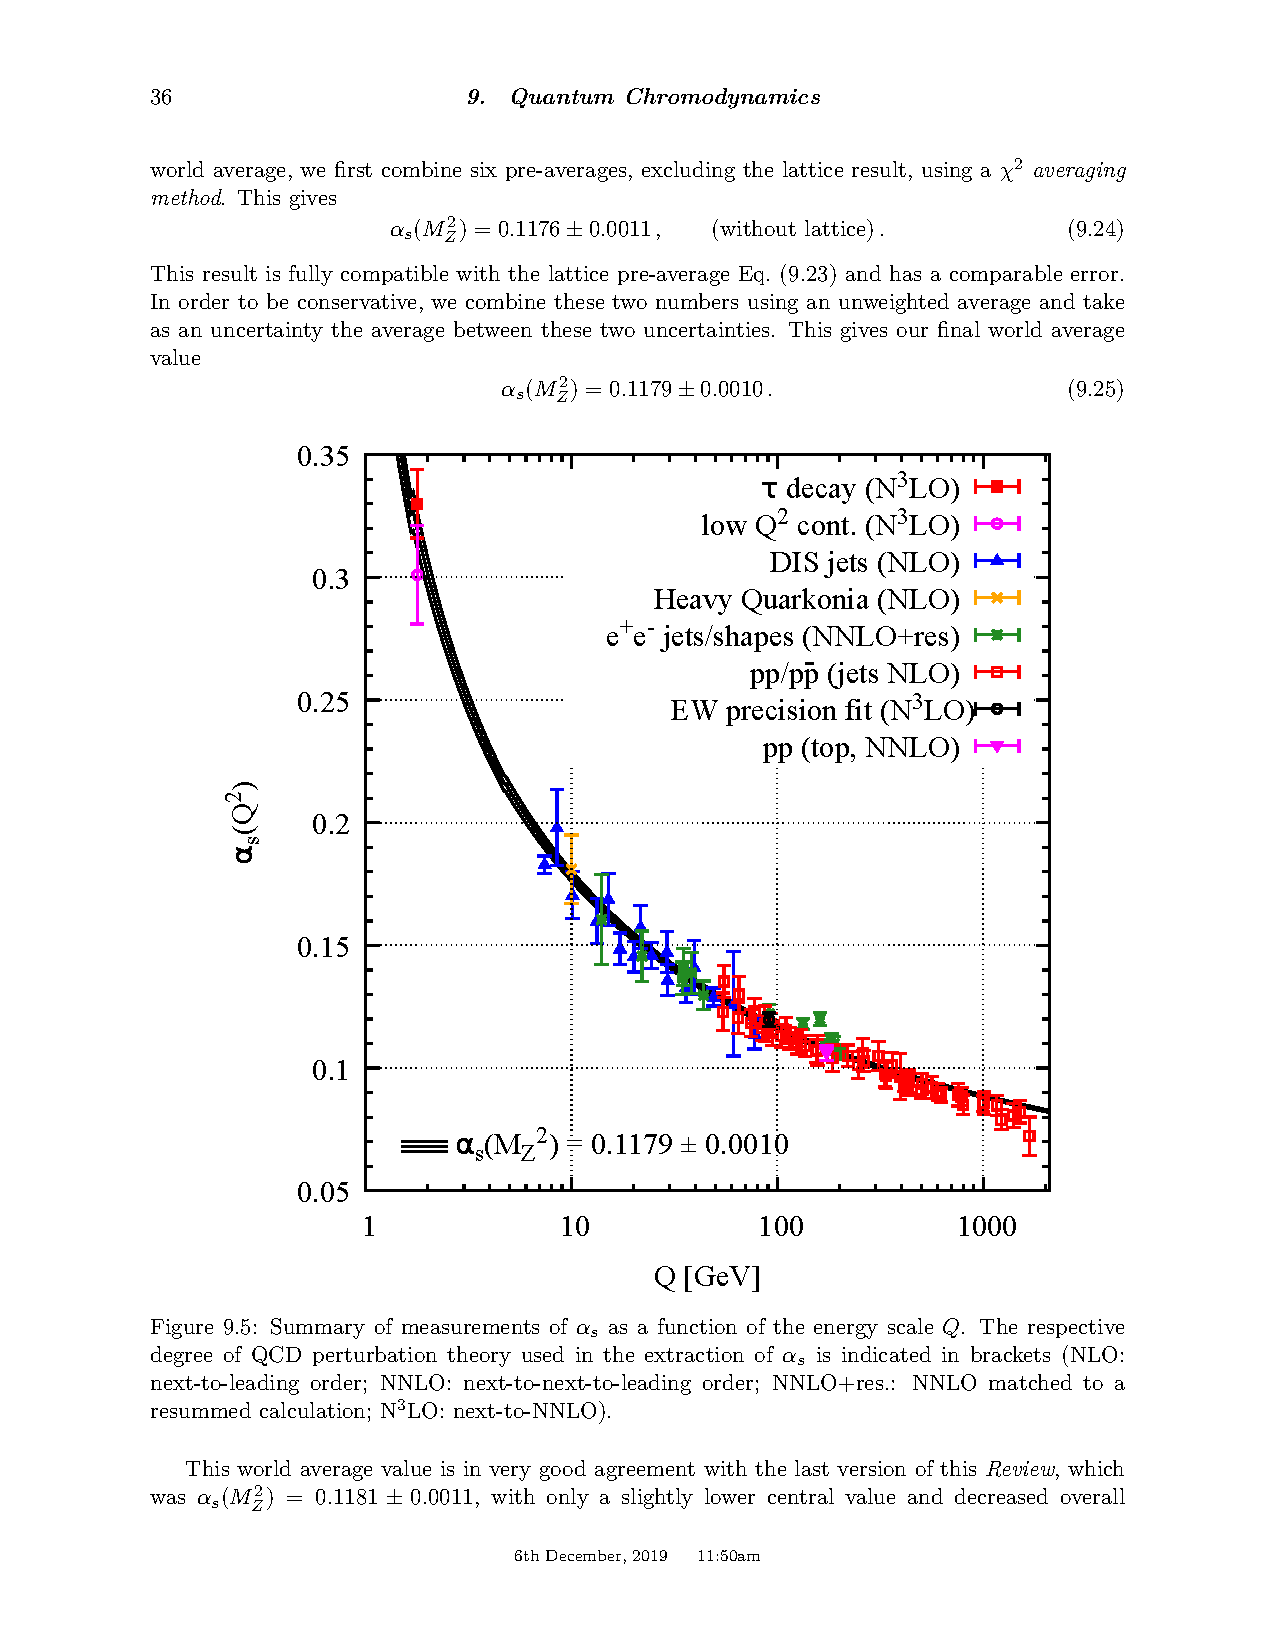
\includegraphics[trim={3.5cm 5.9cm 3cm 7cm},clip,width=1.0\textwidth] {Introduction/a_S_running.pdf}
    \caption{The QCD coupling constant, $\alpha_S$, plotted as a function of the momentum scale,  $Q$ for various measurements. The degree of perturbation theory used in the extraction of  $\alpha_S$ is indicated in brackets next to each measurement. The bottom left shows the global average for the coupling strength at the Z boson mass, $Q=M_Z$ \cite{zotero-314}.}
    \label{fig:a_S_running}
  \end{figure}
  

  Thus, we reach yet another important divergence from QED: While in QED, the coupling becomes larger at higher energy, the negative value of b in Eq.~\ref{eq:b} means that in QCD, the coupling becomes smaller at higher energy. This property is known as \textit{asymptotic freedom}, and indicates that at large energy, the interaction between quarks is small. 
  On the opposite end of the scale, for example when the distance between quarks grows large, the energy stored by the field exceeds the threshold for the creation of new matter (in the form of a $q\bar{q}$ pair). This phenomenon is known as \textit{confinement}, and results in the absence of free quarks in nature. They are instead trapped in bound states with a net zero color charge known as mesons containing a quark and an anti-quark, or baryons consisting of three (anti)quarks.

\section{Relativistic Heavy Ion Collisions}\label{sec:rhics}
% The study of high energy nuclear collisions may give us a more complete understanding of how particles are produced via QCD. But this is not a new endeaver, and is a natural extension of the question "how are particles produced in high-energy collisions?" A question that long predates even QCD.
Today, studying ultrarelativistic heavy ion collisions may give us a more complete understanding of how particles are produced in high-energy collisions via QCD, illustrating one of the fundamental interactions of nature. The history of nuclear collisions, however, predates the parton model, and even QCD itself. The first dedicated heavy-ion accelerator, the Heavy Ion Linear Accelerator (HILAC) began operation in 1957 in Berkeley, CA. At the time, the primary objectives of the field were nuclear transmutation and the investigation of radiation damage to human tissue for space travel. HILAC could accelerate ions as heavy as Argon up to 10 MeV \cite{AIP2014}. A few years later, Gell-Mann and Feynman's parton model was verified by deep inelastic scattering experiments at SLAC, but it was not until the 70's that the theory of QCD was steadily developed. The idea of asymptotic freedom was discovered by David Gross and Frank Wilczek, and independently by David Politzer in 1973, who shared the Nobel prize 2004. Based on this idea, J. C. Collins and M. J. Perry of Cambridge predicted that at sufficiently high densities, long-range interactions would be effectively screened and nuclear matter would behave as an ideal gas of quarks and gluons \cite{Collins1975}. %Edward Shuryak and others would expand on these ideas using the machinery of finite temperature field theory to hot, dense matter.  

This would mark a fundamentally new state of matter, the Quark Gluon Plasma (QGP). The study of this state of matter has became one of the primary goals of nuclear physicists and has helped motivate the construction the Relativistic Heavy Ion Collider (RHIC) as well as upgrades to the LHC \footnote{The construction of the LHC was of course primarily motivated by the search for the Higgs Boson, lead by CMS and ATLAS, but the construction of A Large Ion Collider Experiment (ALICE) were motived by the study of QGP}. The upgraded LHC is capable of colliding Lead ions with a center of mass energy per nucleon, \sqrtsNN, of 5.02 TeV. A considerable step up from Argon ions at 10 MeV. 


% QGP temperature. Because of this, observed modifications to observables attributed to the production of quark gluon plasma are often referred to as "hot nuclear matter effects".
\section{The Quark Gluon Plasma}\label{sec:QGP}

Investigating the QCD phase diagram as a function of both temperature and baryon doping (or net baryon number), is among one of the most important reasons for studying relativistic heavy ion collisions. Figure \ref{fig:qcd_phase} shows the currently understood QCD phase diagram as a function of temperature and net baryon number, parametrized by the baryon chemical potential, $\mu_B$.

\begin{figure}[htpb]
  \centering
  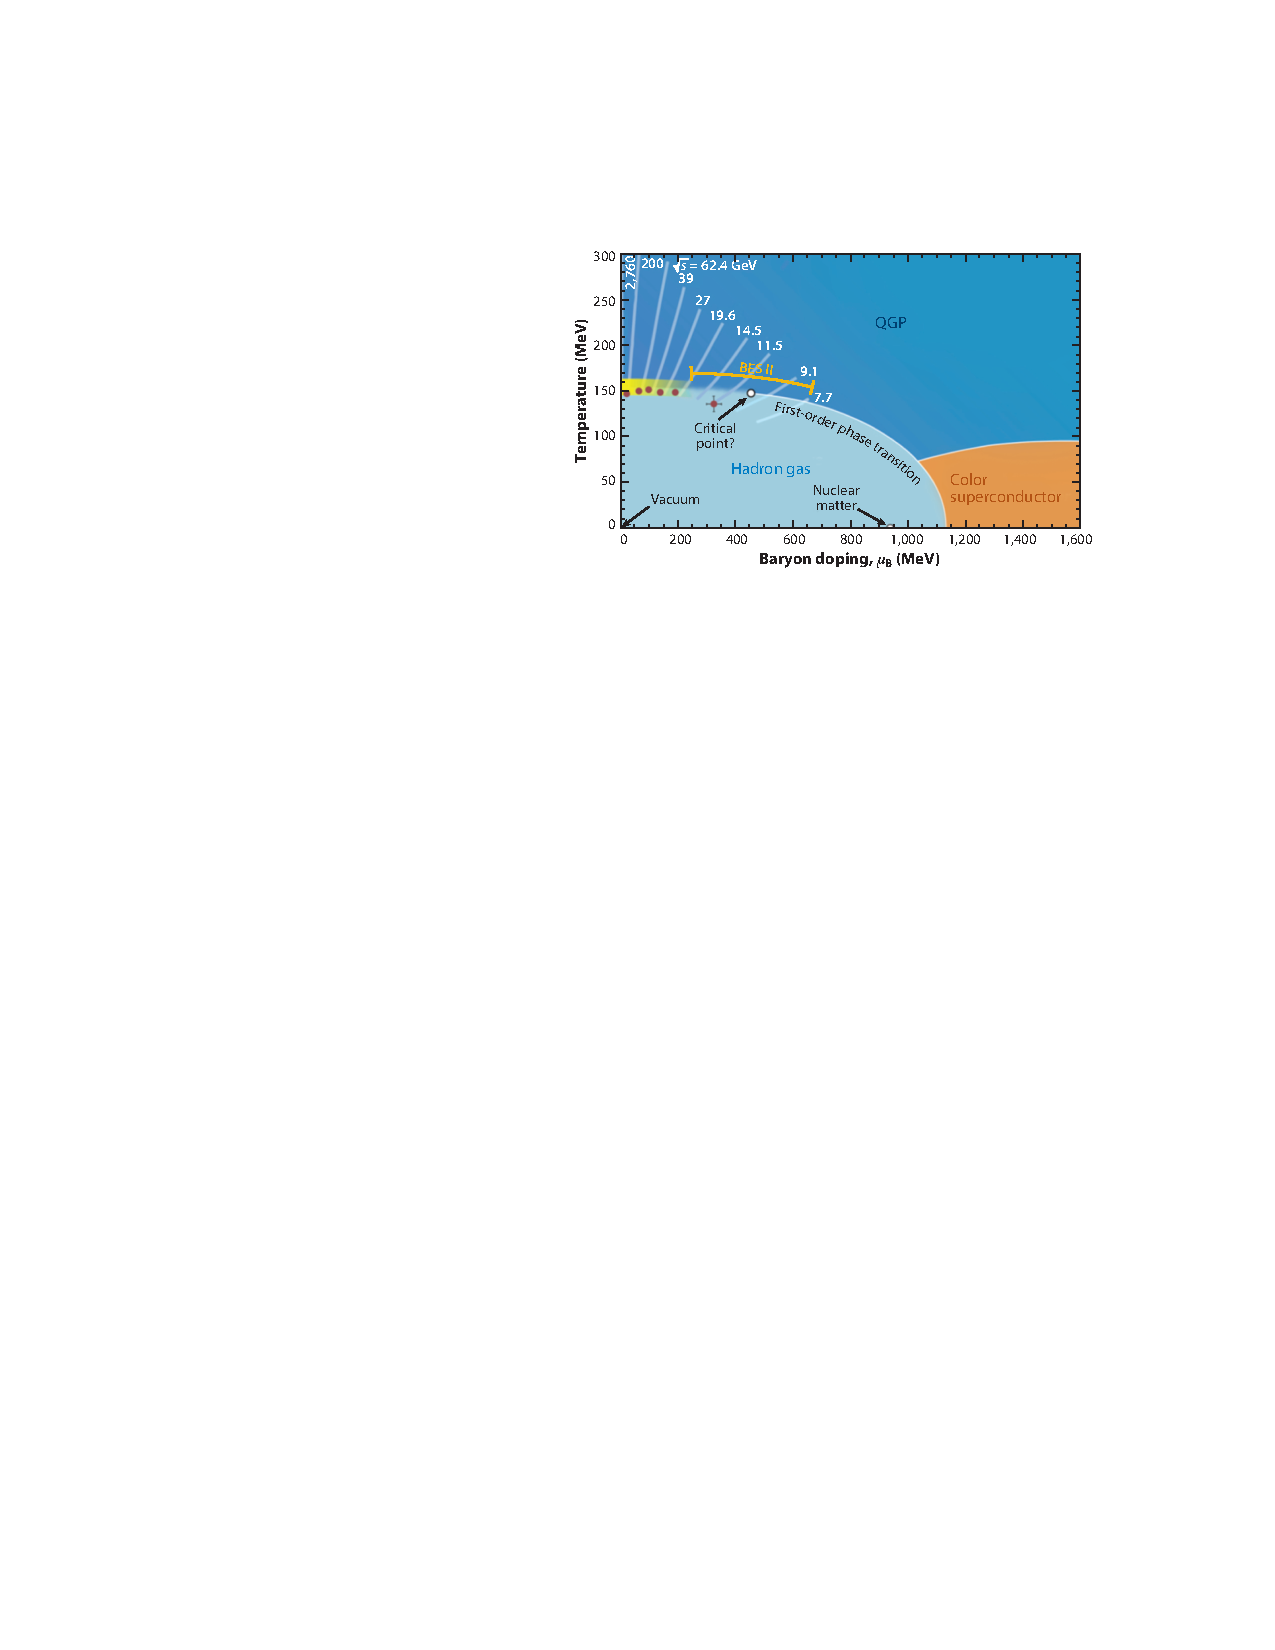
\includegraphics[width=.99\textwidth]{Introduction/qcd_phase.pdf}
  \caption{The current understanding of the expected features of the phase diagram of QCD as a function of temperature and baryon doping, the excess of quarks over antiquarks.\cite{annurev-nucl}.}
\label{fig:qcd_phase}
\end{figure}

At the extremely high density and pressure, achieved in relativistic heavy ion collisions, quarks and gluons are no longer bound within hadrons, instead they are characterized by astate of \textit{deconfinement}. The maximum energy density occurs shortly after the two highly Lorentz-contracted nuclei collide.  This system is of course not in equilibrium instantaneously, and the large energy density is a consequence of the Lorentz contraction of the lead nuclei. In PbPb collisions, equilibrium is predicted to occur at approximately around 1 fm/$c$, where the energy density is 12GeV/fm$^3$, about 20 times the energy density inside hadron at 500 MeV/fm$^3$ \cite{annurev-nucl}. Figure~\ref{fig:collision_snapshot} shows snapshots of a PbPb collision at different times \cite{annurev-nucl}. The figure shows two highly lorentz contracted nuclei right before they collide, followed by a snapshot of a very dense system of QGP, and ending with the production of final state hadrons several fm/$c$ after the collision. While the temperature of the QGP varies by collision system and energy, it is thought that QGP formed at RHIC in AuAu collisions reaches temperatures of 300 MeV, with the higher temperatures obtained in PbPb collisions at the LHC \cite{annurev-nucl}. The quarks and gluons produced in the collision cannot be described as a system of distinct hadrons. That is not to say, however, that the quarks and gluons in this high-energy-density matter are independent. After production, the QGP expands until the energy density of the plasma drops below that within an individual hadron and the fluid falls apart into a mist of hadrons (known as "chemical freeze-out"). These hadrons then scatter off one another a few times until they propagate freely in a process known as "kinetic freeze-out" \cite{annurev-nucl}.

\begin{figure}[htpb]
  \centering
  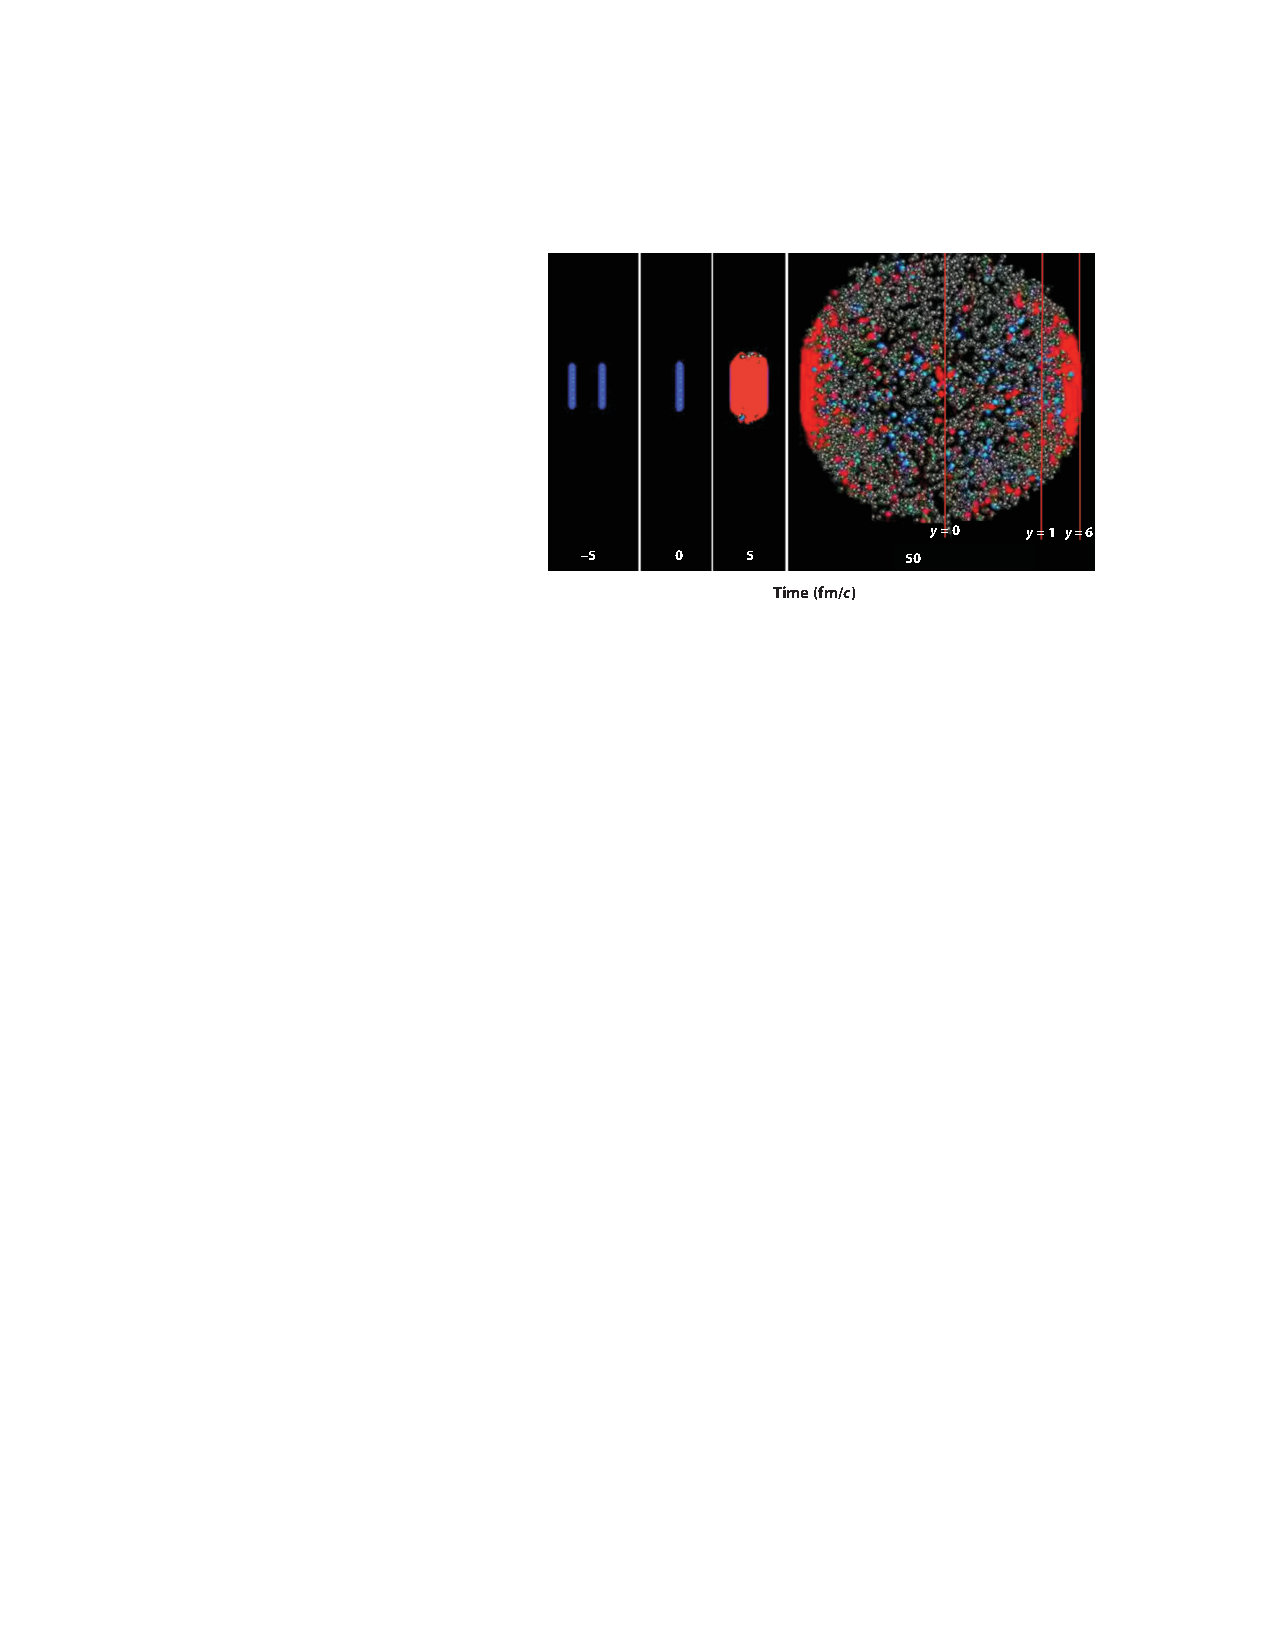
\includegraphics[width=0.99\textwidth]{Introduction/collision_snapshot.pdf}
  \caption{Snapshots of a central 2.76 TeV PbPb collision at different times with hadrons (blue and gray spheres) as well as quark gluon plasma (red). The red vertical lines indicate different regions of rapidity \cite{annurev-nucl}.}
  \label{fig:collision_snapshot}
\end{figure}
While the prediction of a QGP state is based on perturbative ideas, its properties cannot be estimated perturbatively -- enter lattice QCD. In the 1970's, a method was discovered where QCD may be calculated computationally at large scales by replacing continuous space with a finite lattice~\cite{Wilson1974}. Lattice QCD is a non-perturbative approach to solving QCD, and when the size of the lattice is taken to be infinitely large and its sites infinitesimally close to each other, the continuum QCD is recovered. Figure~\ref{fig:lattice_qcd} shows lattice QCD calculations for the  pressure p, energy density $\epsilon$, and entropy density s of hot QCD matter in thermal equilibrium at temperature T \cite{Borsanyi2014,HotQCDCollaboration2014}. Lattice QCD gives several powerful insights on the order of the phase transition from hadronic matter to a quark gluon plasma, the critical temperature at which the phase transition occurs, approximately $T_C\approx$200 MeV, as well as the bulk properties of the system shown in Fig.~\ref{fig:lattice_qcd}. Lattice QCD has strict limitations, however. Aside from requiring huge amounts of high performance computing, lattice calculations are built upon the Euclidean formulation of equilibrium thermodynamics, and so it is much more challenging to use them to gain information about transport coefficients such as the shear and bulk viscosities, new techniques are required to describe time-dependent processes of the plasma. There has been recent progress, in \cite{Kumar2021}, where the transport coefficient of partons propagating through the medium has been calculated using lattice QCD.


\begin{figure}[htpb]
  \centering
  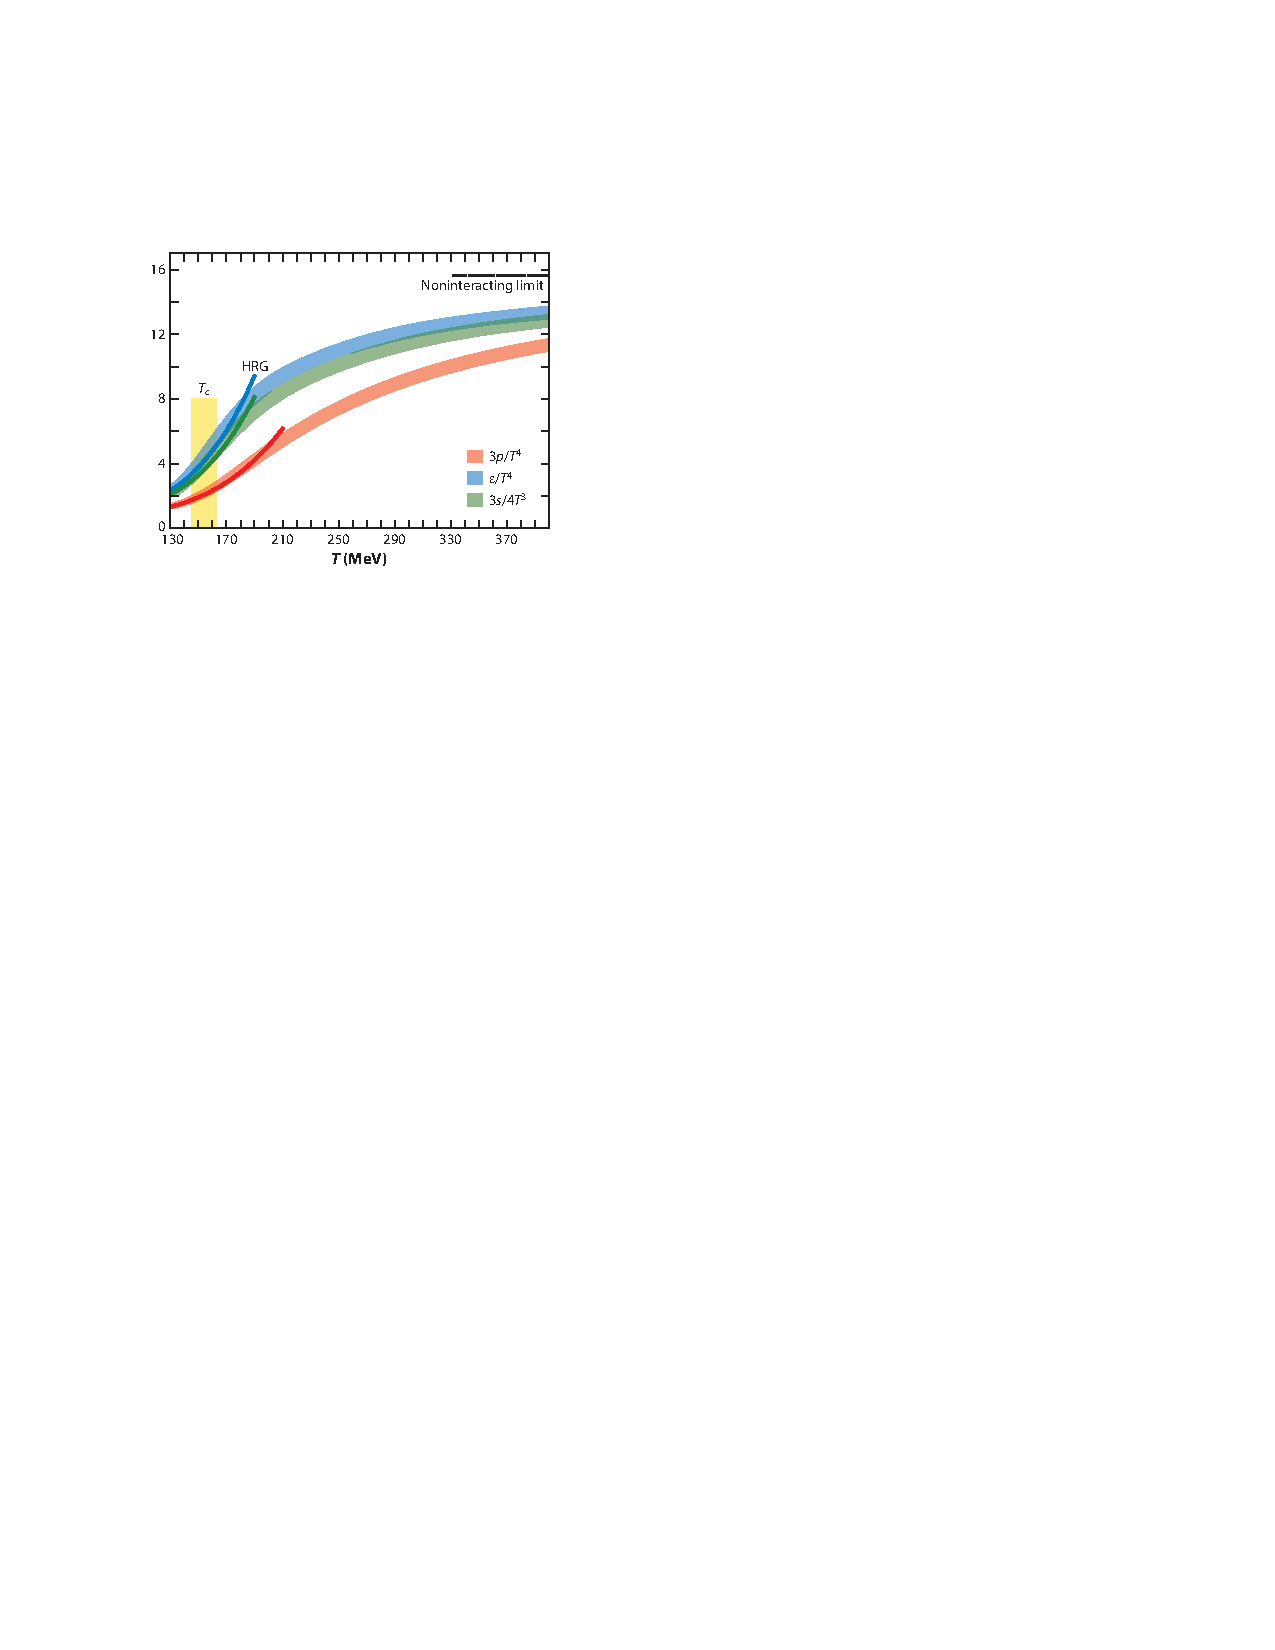
\includegraphics[width=0.8\textwidth]{Introduction/lattice_qcd.pdf}
  \caption{Lattice QCD calculations (colored bands) of the pressure p, energy density $\epsilon$, and entropy density $s$ of hot QCD matter in thermal equilibrium at temperature T and small but non-vanishing baryon chemical potential \cite{Borsanyi2014,HotQCDCollaboration2014}. The figure shows a continuous crossover around T$\approx$150 MeV, from a hadron resonance gas (HRG; colored lines) at lower temperatures to quark–gluon plasma (QGP) at higher temperatures. This transition is expected to a cross-over phase transition, as indicated in the low $\mu_\mathrm{B}$~region in Fig.\ref{fig:qcd_phase} \cite{annurev-nucl}.}
  \label{fig:lattice_qcd}
\end{figure}


While Perturbative QCD (pQCD) and lattice QCD calculations have their limitations, in conjunction with the discovery of asymptotic freedom, they all point towards the formation of a state of matter made up of deconfined quarks and gluons. In the next section, experimental evidence of the creation of such a state of matter will be discussed. 

\subsection{Collective Flow}\label{sec:flow}

The original extension of asymptotic freedom suggested that the deconfined state of quark and gluons at high energy densities would behave as an ideal gas (see the right hand siged of Fig.~\ref{fig:lattice_qcd}, at the non-interacting limit). In fact, the interplay between two key features of QCD determines the nature of this state of matter. First, because of asymptotic freedom and the high energies probed at RHIC and the LHC, it could be that the interactions between the partons are so weak that the system may never reach thermal equilibrium. Second, at energy scales within an order of magnitude of the confinement/deconfinement energy scale, QCD is strongly coupled. It was only recently been realized after the experiments at RHIC that in this temperature range QCD describes a relativistic fluid consisting of quarks and gluons that are so strongly coupled to each other that the resulting liquid cannot be described in terms of a gas of free particles \cite{ADCOX2005184,ADAMS2005102,BACK200528,ARSENE20051}. The weak coupling picture must be correct during the initial stages of the collisions with exceedingly high energy; yet even in these collisions, the strong coupling picture becomes applicable at later times, after a hydrodynamic fluid has formed. The time of the initial moments of the collisions at RHIC or the LHC where the weakly coupled picture can be applied remains an open question.
%The v2 in small systems also brings into questions the equilibrium timescale to reach equilibrium, and has also spawned a new set of questions on pre-equilibrium hydrodynamics \cite{Romatschke2018}

% On the other hand, if the quarks and gluons form a strongy coupled liquid relatively quickly, the fluid will expand hydrodynamically, where hydrodynamics will convert initial spatial anisotropies to into momentum anisotropies.

As the colliding nuclei do not usually hit directly head on, there is a non-symmetric overlap region of the two nuclei. This is shown in Fig.~\ref{fig:overlap}, where the cartoon shows the resulting elliptically shaped overlap region produced when two spherical nuclei are involved in a more peripheral collision. This causes a pressure gradient, which in turn causes more particles to flow along the direction of the reaction plane, defined by the beam direction and impact parameter (vector connecting the centers of the two nuclei). The reaction plane is shown as the green grid in Fig.~\ref{fig:overlap}.

\begin{figure}[htpb]
  \centering
  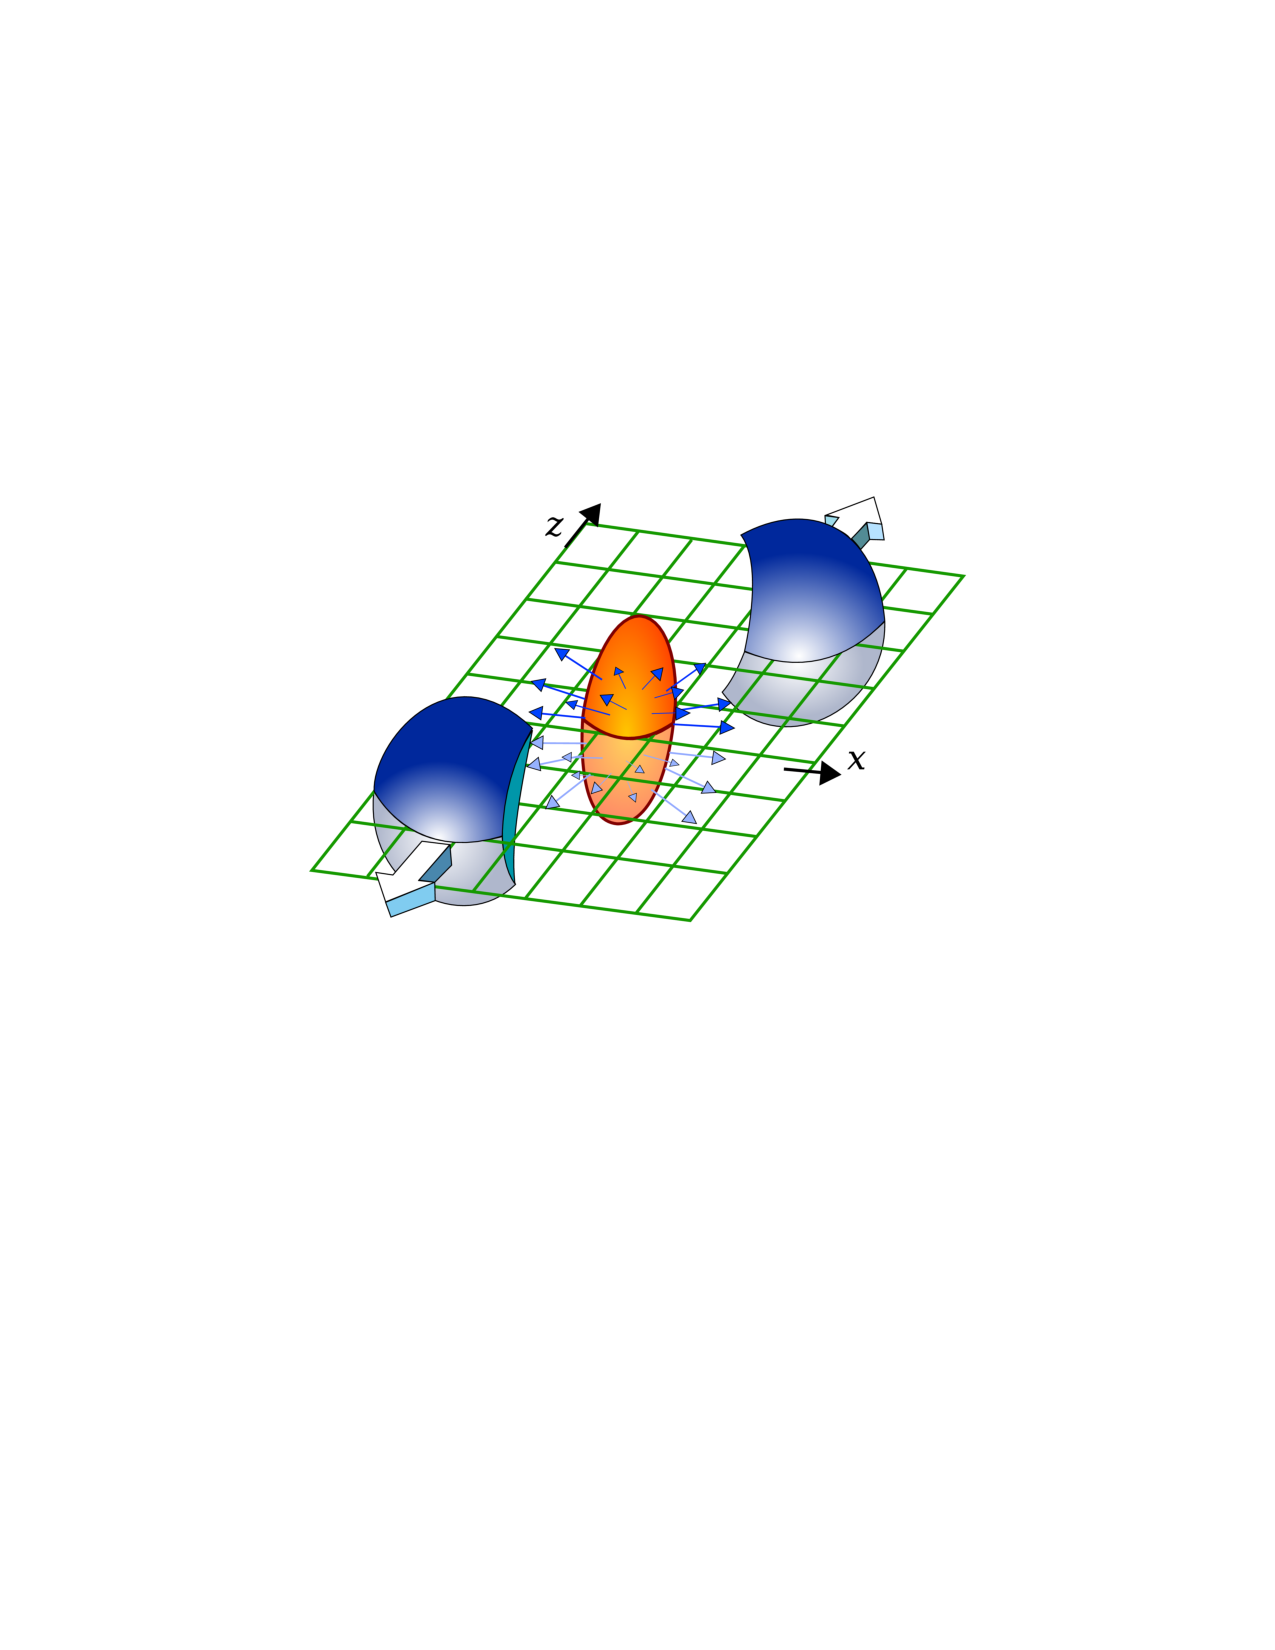
\includegraphics[width=0.8\textwidth]{Introduction/overlap_diagram.pdf}
  \caption{The reaction plane of the collision is shown here for a collision in which the overlap region has an almond-like shape. This spatial anisotropy in the initial collisions results in a flow of particles in the direction of the reaction plane. The reaction plane is defined by the direction of the beams, $z$, and the impact parameter which connects the centers of the colliding nuclei and happens to be along the $x$ direction in this plot \cite{Masui}.}
  \label{fig:overlap}
\end{figure}

By measuring the anisotropy of particles produced in heavy ion collisions, the crucial distinction between these two scenarios can be found: In the case of a weakly interacting gas of particles, the initial spatial anisotropy of the collision zone would essentially be washed out by random motion, leaving the azimuthal distribution of final state particles roughly isotropic. Alternatively, if the quarks and gluons form a strongly coupled liquid soon enough, while the distribution of energy density produced in the collision remains anisotropic, this noncircular and lumpy drop of fluid will expand in a hydrodynamic fashion, yielding faster expansion in the direction of larger gradients: Hydrodynamics converts spatial anisotropies into momentum anisotropy.

A Fourier analysis is performed to relate the measured angular distribution of final state (charged) particles to the azimuthal momentum anisotropy. This Fourier analysis is shown in Eq. \ref{eq:vn}:

  \begin{equation}
    \frac{\mathrm{d}\bar{N}}{\mathrm{d}\varphi} = \frac{\mathrm{d}\bar{N}}{2\pi} \left(1 + 2\sum^\infty_{n=1}\bar{v}_n\cos[n(\varphi - \bar\Psi_n)]\right)
    \label{eq:vn}
  \end{equation}
with $\varphi$ the azimuthal angle centered about the beam axis, $\bar\Psi_n$ are the event plane angles determined with respect to the beam direction, and $\bar{N}$ is simply the average number of particles in the event. Importantly, $\frac{\mathrm{d}\bar{N}}{\mathrm{d}\varphi}$ is the quantity that is directly measured, and $v_n$ is extracted as a fourier coefficient that quantifies the magnitude of flow. The subscript $n$ indicates the order of the harmonic, with $v_n$ indicating the kind of flow and are thus called \textit{flow coefficients}. For example, $v_1$ corresponds to radial flow, and perhaps more interestingly, $v_2$ corresponds to elliptic flow that results from the initial elliptic overlap region shown in Fig~\ref{fig:overlap}. $v_2$ has been measured extensively at RHIC and the LHC, and has been showed to be non-zero and positive. This strongly indicates that the picture of a strongly coupled fluid that is formed proceeding the initial collision is the correct picture.  

  
  This cartoon is of course a simplification: the nuclei are made up of nucleons (in turn made of partons) and are quite lumpy, resulting in more complex spatial anisotropies in the initial collision, and therefore higher order flow coefficients. The interacting partons move around within the nucleons before the initial collision. This can give rise to different overlap shapes, which can result in non-zero measurements of higher order flow harmonics. This is demonstrated beautifully at a larger scale in Fig.~\ref{fig:collision_geometries}, where different nuclei of distinct shapes, $^3$He, deuterium, and protons, are simulated as they collide with Au, yielding simple yet very distinct collision geometries \cite{Aidala2019}. 

  \begin{figure}[htpb]
    \centering
    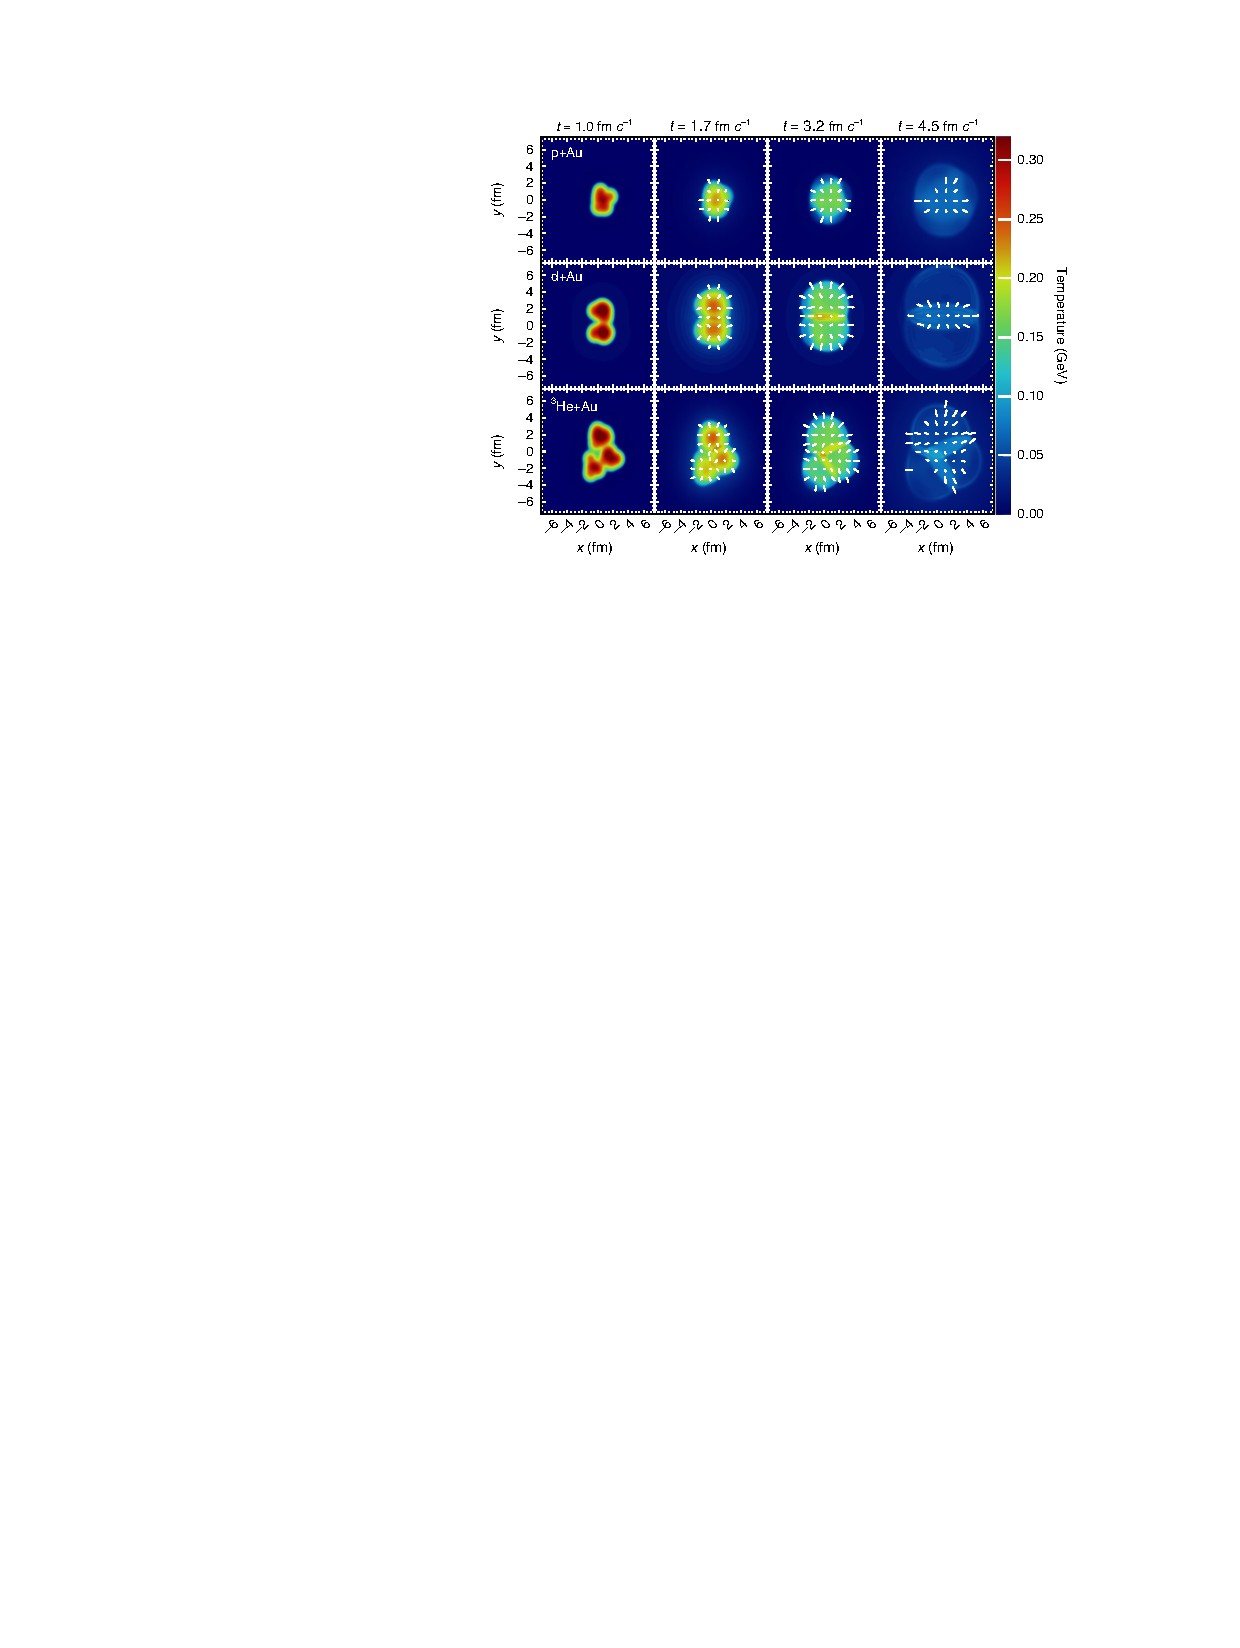
\includegraphics[width=0.8\textwidth]{Introduction/collision_geometries.pdf}
    \caption{Hydrodynamic evolution of a typical head-on p+Au (top), d+Au (middle) and $^3$He+Au (bottom) collision at $\sqrt{s_\mathrm{NN}}$ = 200 GeV as calculated by SONIC, where the $p/d/^3$He completely overlaps with the Au nucleus. From left to right each row gives the temperature distribution of the nuclear matter at four time points following the initial collision at t = 0. The arrows depict the velocity field \cite{Aidala2019}.}
    \label{fig:collision_geometries}
  \end{figure}

  The bottom most panel would correspond to an larger $v_3$ measurement. Higher flow harmonics in larger systems (AA and PbPb) have been measured as well. Fig \ref{fig:flow_measurements} shows such measurements up to $v_5$ \cite{Aamodt2011}, illustrating that the movement of nucleons (rather than nuclei with distinct shapes in Fig.~\ref{fig:collision_geometries}) can yield measurements of higher order flow harmonics. 

  \begin{figure}[htpb]
    \centering
    \raisebox{0.6cm}{ 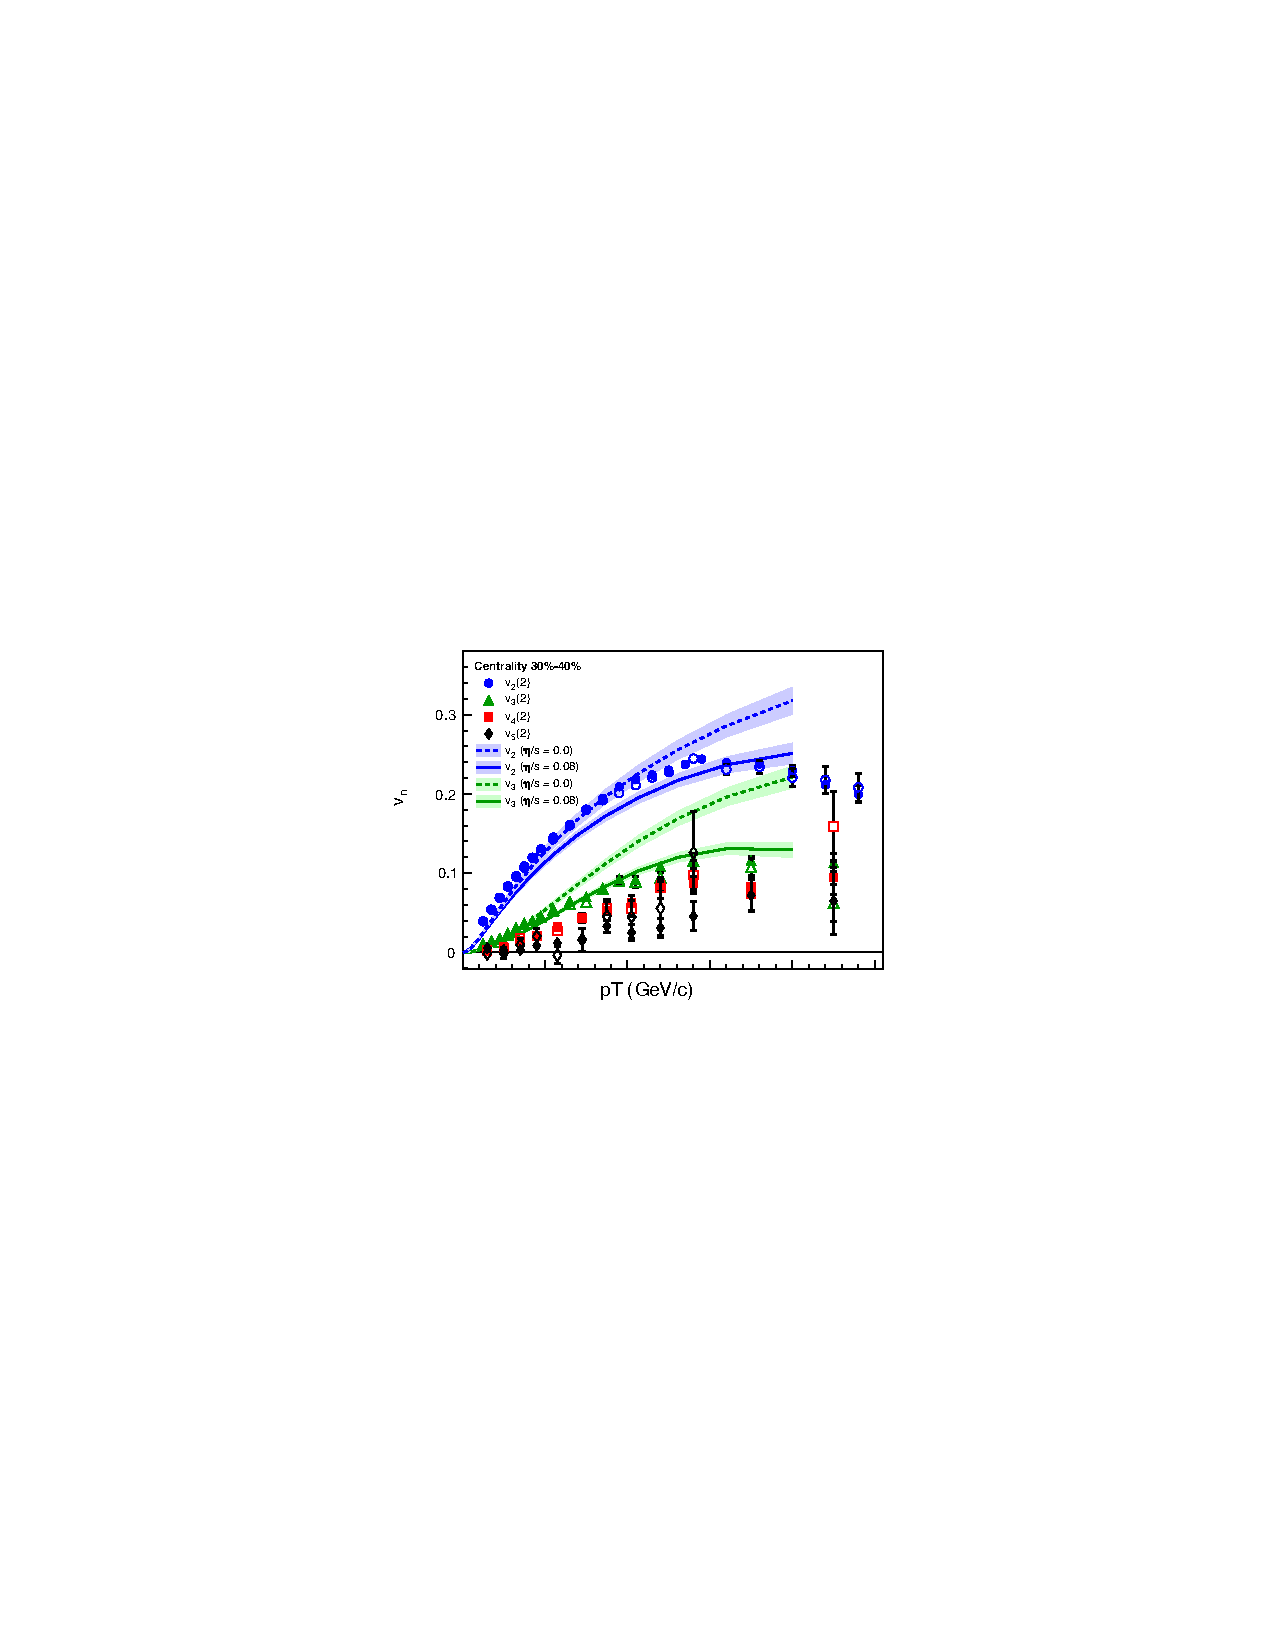
\includegraphics[width=0.45\textwidth]{Introduction/flow_measurements_peripheral.pdf} }
    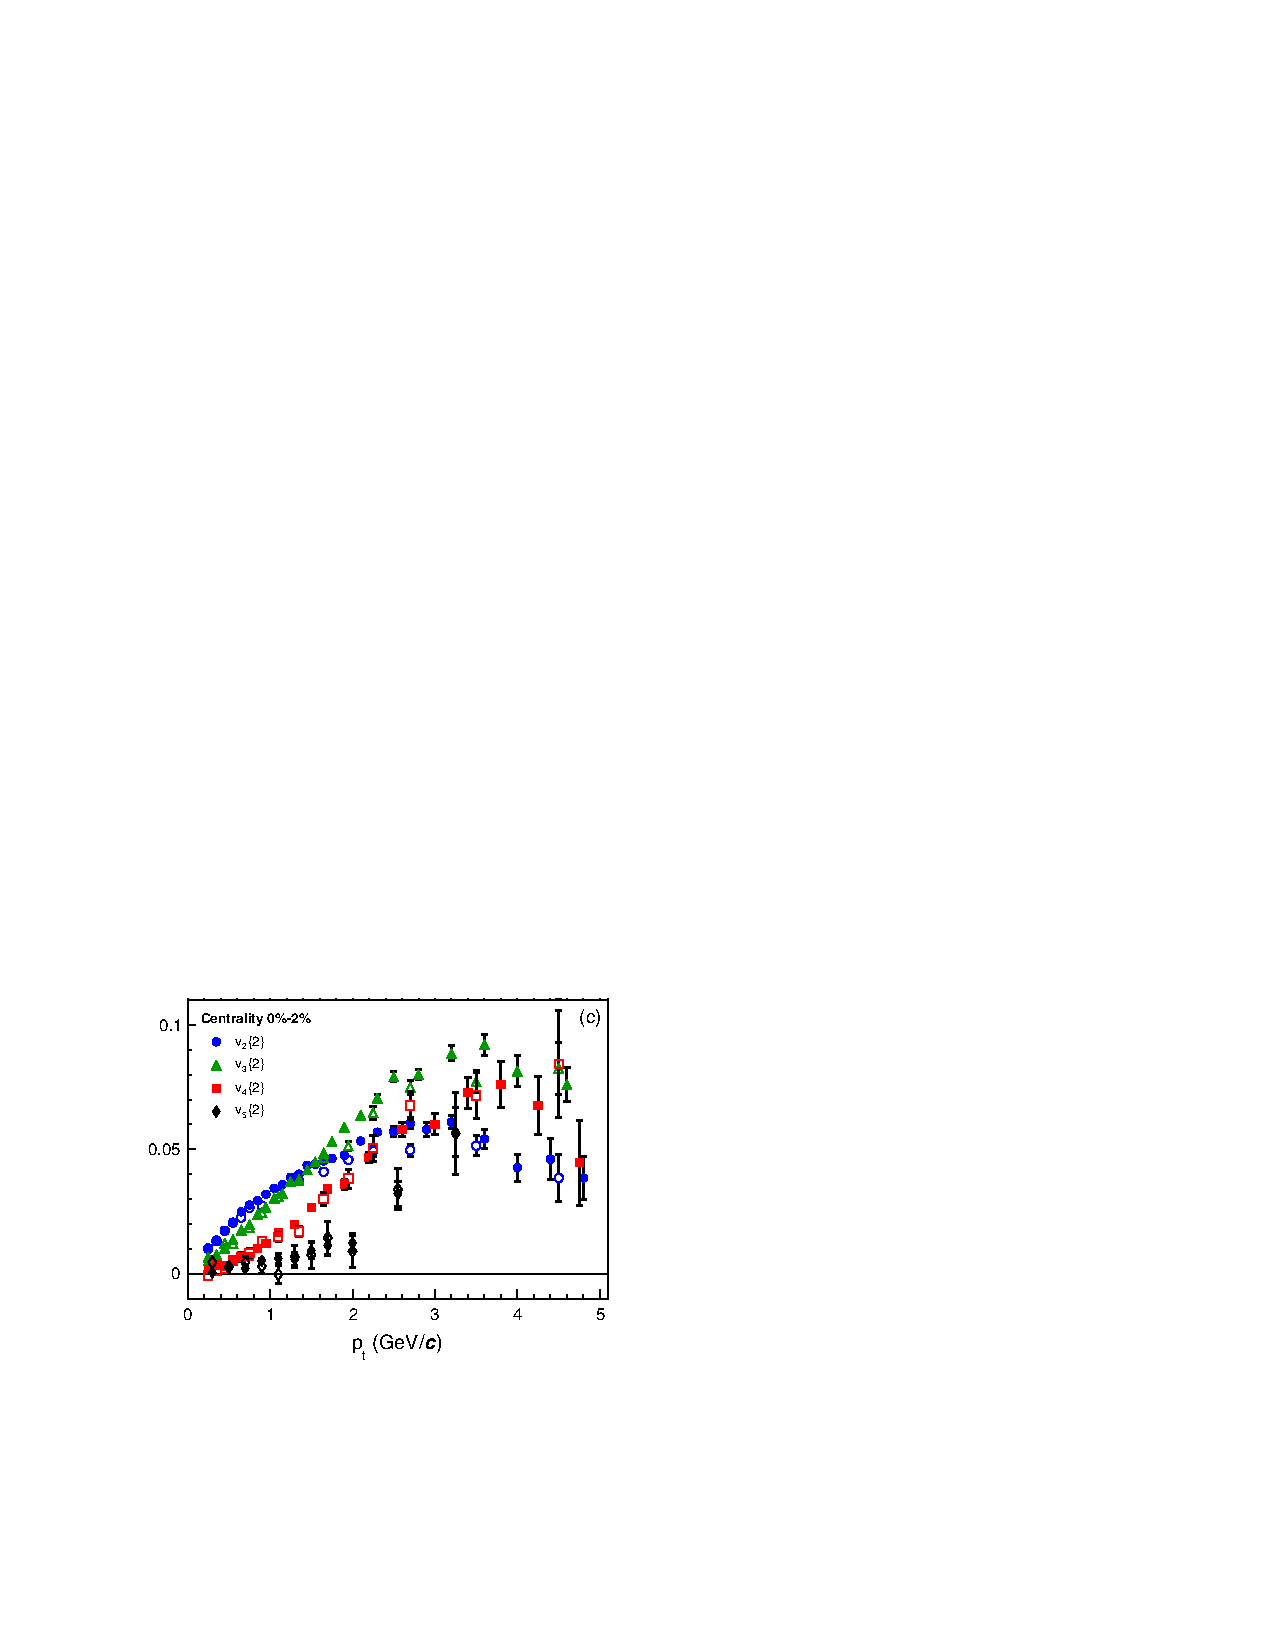
\includegraphics[width=0.45\textwidth]{Introduction/flow_measurements_central.pdf}
    \caption{$v_2, v_3, v_4$, and  $v_5$ as a function of particle transverse momentum, \pt, for peripheral (left) and central (right) PbPb events. The full and open markers are for  $\Delta\eta < 0.2$ and  $\Delta\eta < 1.0$, respectively. The colored bands represent hydrodynamic models with two different parameters for the specific viscosity \cite{Aamodt2011}.}
    \label{fig:flow_measurements}
  \end{figure}


  The property that quantifies the liquidness of a material made up of ultrarelativistic constituents is the ratio of its shear viscosity $\eta$ to entropy density, $s$, whcih is the entropy per particle in systems with fixed number of particles. The ratio $\eta/s$ is dimensionless in units where $k_B$ and $\bar{h}$ have been set to 1. This ratio plays a key role in the equations of hydrodynamics which govern the effects of shear viscosity in a relativistic fluid, and is often called the ``specific viscosity''. The precise magnitude of the anisotropies $v_n$ should then be quite sensitive to the viscosity of the plasma. Specific viscosity controls how rapidly gradients of any sort introduced in the initial conditions are dissipated into heat. This means that flow measurements compared to theory calculations can constrain the specific viscosity. By using simulations with smooth initial conditions (obtained from lattice calculations),  it can be estimated that the specific viscosity of the QGP is approximately 0.08-0.20 \cite{Romatschke2007}. The lower end of which is remarkably close to the theoretical limit for any liquid of 1/$4\pi$. For this reason, the quark gluon plasma is often called the most perfect liquid.

 % meaning that it is this quantity which is ultimately constrained by comparing hydrodynamic calculations with data
 % Alternatively, if the quarks and gluons form a strongly coupled liquid soon enough, while the distribution of energy density produced in the collision remains anisotropic, this noncircular and lumpy drop of fluid will expand in a hydrodynamic fashion, yielding faster expansion in the direction of larger gradients: Hydrodynamics converts spatial anisotropies into momentum anisotropy

% Specific viscosity controls how rapidly gradients of any sort introduced in the initial conditions are dissipated into heat, meaning that it is this quantity is ultimately constrained by comparing hydrodynamic calculations with data.

\subsection{Jets}
The next key piece of evidence for the production of a hot, deconfined nuclear matter has to do with the observed modification of jet production in heavy ion collision. But before discussing this observable, it will be useful to discuss exactly what a jet is, and perhaps more fundamentally, how partonic interactions are related to experimental observables such as the data in Fig.~\ref{fig:a_S_running}. Generally, the perturbative regime of QCD is explored using high energy collisions of elementary particles, the simplest of which are electron-positron collisions. In these collisions, quarks may be produced in the final state by the reaction $e^++e^- \rightarrow q\bar{q}$. Yet, due to confinement these quarks are not observed at the detector level, but rather hadronize into a collimated spray of mesons and baryons, which are correlated in phase space and collectively referred to as \textit{jets}. 

At a high level, a jet represents a virtual hard parton and its subsequent evolution. In practice, a jet is a ``contract'' between experimentalists and theorists': hadrons are combined into jets using specific definitions and reconstruction algorithms (most prominently the \kt, Anti-$k_\mathrm{T}$ and Cambridge/Aachen reconstruction algorithms~\cite{Atkin2015}) cleverly based on pCQD arguments. 

The jet reconstruction algorithms cluster entities (usually measured particles) based on their distance relative to other entities, $d_{ij}$, and compares it to the it's distance from the beam, $d_{iB}$. These quantities are defined as \cite{Cacciari2008}, 

\begin{equation}
\begin{aligned}
d_{i j} &=\min \left(k_{t i}^{2 p}, k_{t j}^{2 p}\right) \frac{\Delta_{i j}^{2}}{R^{2}} \\
d_{i B} &=k_{t i}^{2 p}
\end{aligned}
\end{equation}
where $\Delta_{i j}^{2}=\left(y_{i}-y_{j}\right)^{2}+\left(\phi_{i}-\phi_{j}\right)^{2}$ and $k_{t i}, y_{i}$ and $\phi_{i}$ are respectively the transverse momentum, rapidity and azimuth of particle $i$. $R$ is the maximum radius of the jet in $(\deltaphi-\delta\eta)$ and the parameter $p$ govern the relative power of the energy versus geometrical $\left(\Delta_{i j}\right)$ scales.

For the \kt reconstruction algorithm, $p$ is 1. For Anti-\kt, $p=-1$, and for Cambridge/Aachen $p=0$. The value of $p$ largely changes the ordering of particles clustered into the jet, and impact the shape and make up of the final jet that is reconstructed \cite{Cacciari2008}.

\subsection{Nuclear Modification Factor}
\label{sec:raa}
Jet production and showering in vacuum are well described by pQCD, as shown in the blue triangles and green asterisks in Fig.~\ref{fig:a_S_running}. When a jet is produced in a heavy ion collision, however, the partons in the shower must barrel through the droplet of QGP produced in the same collision. As this happens, the parton should loose energy and forward momentum, as the plasma should be opaque to color charge in the same way a more traditional ionized plasma is opaque to light.  This parton energy loss changes the spectrum of the final jets. Thus a key signature of the formation of a quark gluon plasma in the lab is the observation of this \textit{jet energy loss} or \textit{suppression}. This loss of course, is simply the redistribution of the jets energy to the medium, and must be compared to how jets propagate in 'vacuum' (to which pp collisions is taken as an estimation) in order to be quantified. Accordingly, this suppression is quantified by the nuclear modification factor $R_\mathrm{AA}$. 

  \begin{equation}
    R_\mathrm{AA}(p_\mathrm{T}) = \frac{\mathrm{d}N^\mathrm{AA}/\mathrm{d}p_\mathrm{T}}{\langle N_\mathrm{coll}\rangle\mathrm{d}N^\mathrm{pp}/\mathrm{d}p_\mathrm{T}},
    \label{eq:raa}
  \end{equation}
where $\mathrm{d}N^{xx}/\mathrm{d}p_\mathrm{T}$ is the number of jets (or, in other contexts, particles of a specified type) produced in AA or pp collision. Additionally, the nuclear modification factor is expressed here as a ratio of yields instead of cross sections \footnote{Other nuclear modifications factors are $T_\mathrm{AA}$, which includes the ratio of cross sections, and $I_\mathrm{AA}$, which is a ratio of conditional yields}. $\langle N_\mathrm{coll}\rangle$ is the total number of encounters between left and right moving nucleons, which we call the number of binary collisions. While $N_\mathrm{coll}$ cannot be determined directly from measured cross sections, there is a well-defined theoretical procedure based on the collision geometry of distribution of nucleons inside nuclei called Glauber model calculations \cite{doi:10.1146/annurev.nucl.57.090506.123020} for determining this and other quantities. These quantities include the  number of participating nucleons, and centrality classes (percentile classes of multiplicity, or the total number of particles measured in the event), and collision impact parameter. The impact parameter is the distance between the centers of the colliding nuclei. The smaller the impact parameter, the more overlap there is between the colliding nuclei, and the higher the centrality (which yields more produced particles). The number of binary collisions is applied as an important scaling factor where nuclear collisions are naively modelled to be the sum of many independent p+p collisions. Deviations from this scaling, i.e. a modification factor that deviates from 1, indicate that properties of the nucleus or the creation of a plasma are affecting the measurement.

  $R_\mathrm{AA}$ is the ratio of the observed per-event yield in nuclear collisions to the expected yield. Figure~\ref{fig:atlas_raa} shows $R_\mathrm{AA}$ for PbPb collisions.
  \begin{figure}[htpb]
    \centering
    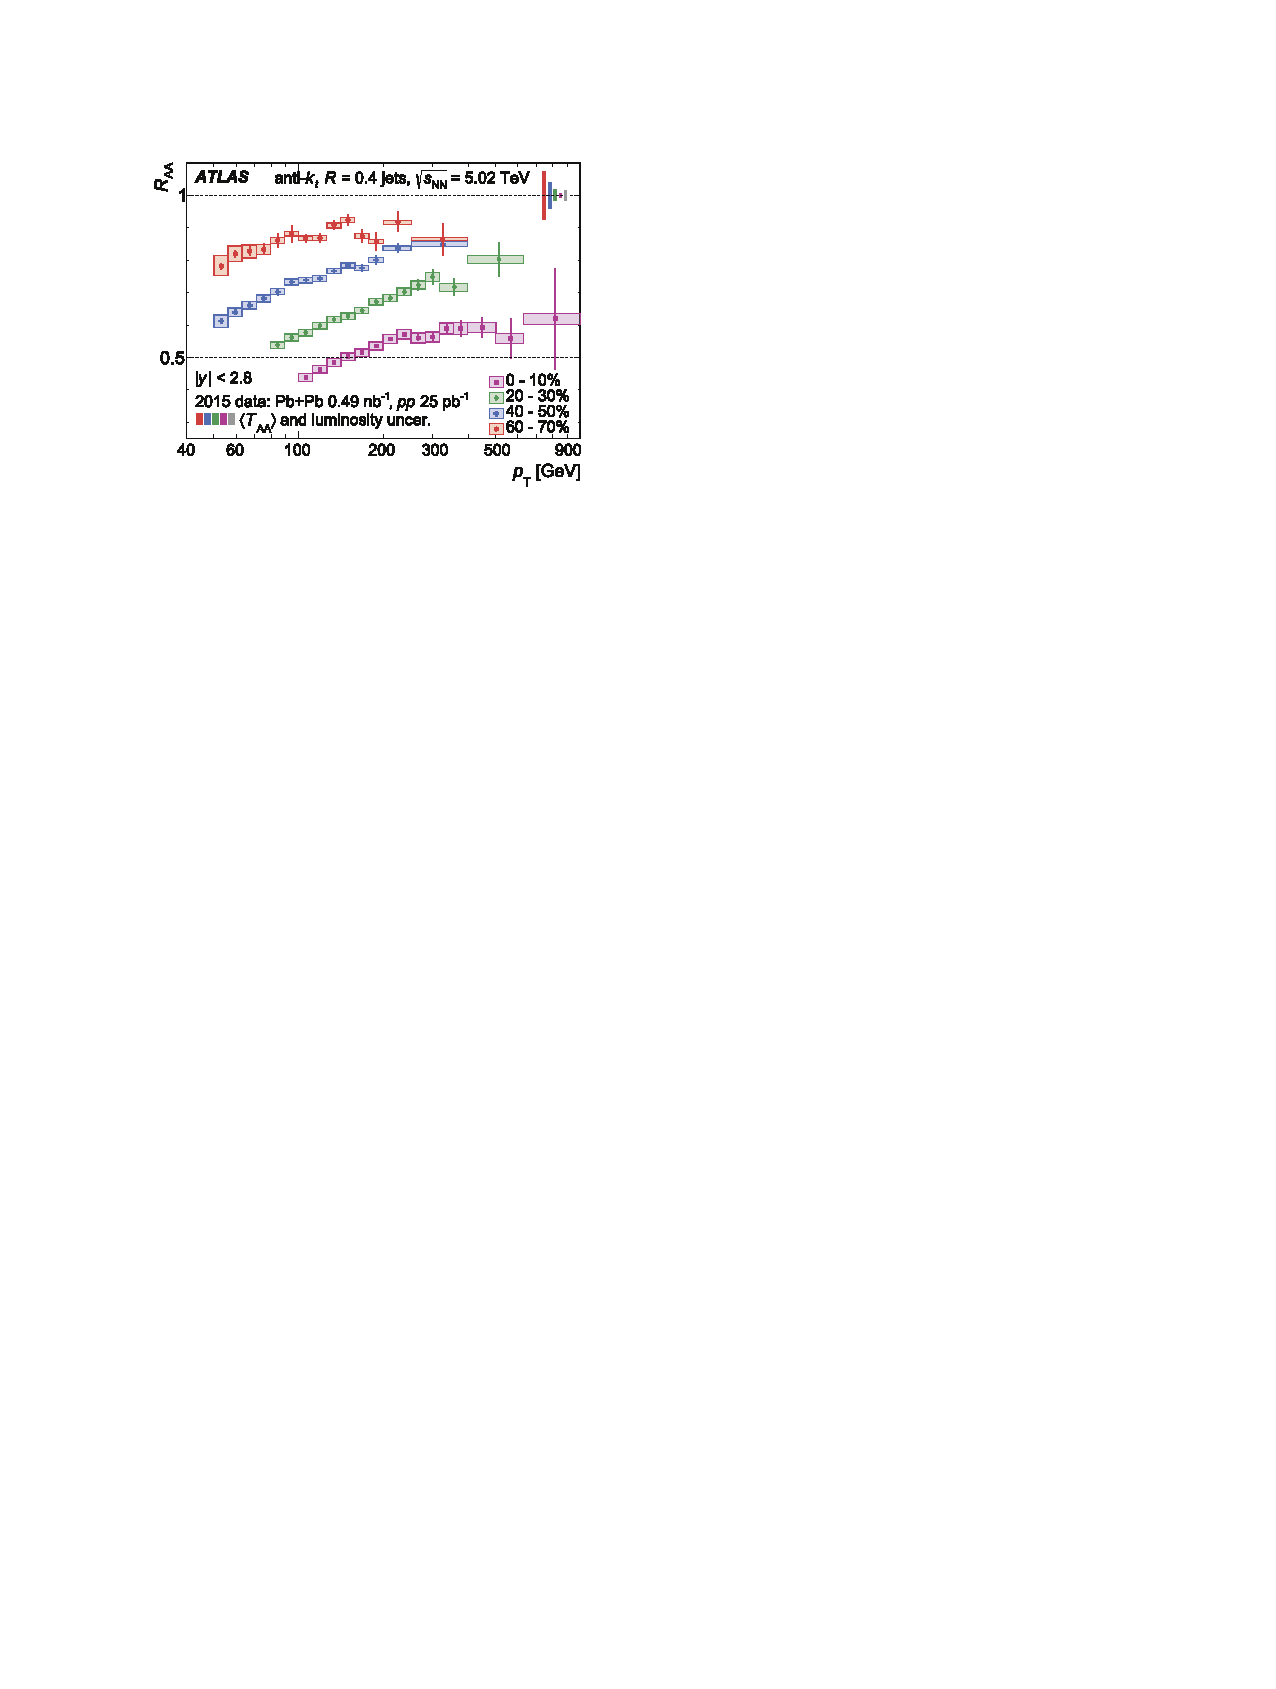
\includegraphics[width=0.8\textwidth]{Introduction/atlas_raa.pdf}
    \caption{The nuclear modification factor $R_\mathrm{AA}$ for jets for four different centralities as a function of jet transverse momentum $p_\mathrm{T}$ \cite{Aaboud2019}. $T_\mathrm{AA} = \langle N_\mathrm{coll}\sigma^{pp}\rangle$}
    \label{fig:atlas_raa}
  \end{figure}
  The amount of suppression shown in Fig. ~\ref{fig:atlas_raa} is quite striking, especially for more central events, where the droplet of QGP that the jets need to traverse is largest. This measurement indicates the formation of a medium that is opaque to color charge, and the measurment points to the suppression of high \pT~ partons. It is considered an extremely important piece of evidence towards the creation of the quark gluon plasma in relativistic heavy-ion collisions \footnote{More precisely, the measured suppression reflects the density of partons in the system, but not necessarily whether the partons are deconfined.}. 

  It is important to realize, however, that high-$p_\mathrm{T}$ jets are produced with a probability that drops rapidly with increasing \pT \cite{Acharya2020}. The steepness of the energy spectrum implies that a small fractional jet energy loss corresponds to a large suppression in $R_\mathrm{AA}$ for jets (this is often referred simply as a ``bin-migration'' effect). This means higher jet \pT~ bins have much lower $R_\mathrm{AA}$ values since each jet that de-populates that bin represents a larger fraction of the total bin count than at lower \pT. In reality, different jets with the same initial energy lose very different amounts of energy, as discussed below, meaning that this argument must be made at the ensemble level. However, the conclusion is the same: the steepness of the jet energy spectrum means the suppression in $R_\mathrm{AA}$ for jets is a very sensitive measure of jet energy loss. 
  % This argument, however, does not apply in the same way for $R_\mathrm{AA}$ measured for single particles.
% The production probability for jets produced at midrapidity scales roughly as $\pT^{-6}$ \ref{annurev-nucl}, for jets with \pT~ values that are not within an order of magnitude of the beam energy.
  The trend for each centrality class is roughly the same, however, where jets at higher \pT~ have modification factors closer to 1. Because of the steepness of the jet spectrum described above, the ensemble of high \pT~ jets that comes out of the droplet of QGP will be dominated by those jets that lost relatively little energy. To put it another way, there are fluctuations in how much energy each individual parton will lose in the medium, and selecting jets which look like high \pt jets in a vacuum may skew measurements towards partons which have lost the least energy in the medium. This is often called the ``survivor bias''~\cite{Connors2018}.

  Figure~\ref{fig:raa_particles} shows the $R_\mathrm{AA}$ measured for a variety single particles \cite{Bencedi2016} measure by ALICE and CMS. The single particle $R_\mathrm{AA}$ distributions provides several insights. First, for the bosons measured in the figure, the $R_\mathrm{AA}$ is consistent with unity. This is a vitally important check to validate the definition $R_\mathrm{AA}$ and the scaling of cross sections using Glauber calculations, as these particles are not expected to interact with the medium. This will be discussed in more detail in \ref{sec:prompt}. Second, the shape: while an overall suppression is seen, the peak at low \pt~is more likely the result of cold nuclear matter effects, i.e. changes due to the presence of the lead nucleus alone in pPb collisions, instead of hot nuclear matter (QGP). The third insight is the shape at high \pT. Note that measuring $R_\mathrm{AA}$ for high-\pT~ hadrons is quite different: in both pp and AA collisions, a high-\pT~ hadron is statistically likely to come from a specific, unusual type of jet that contains one very hard parton and is very narrow. More narrow final state jets are predicted to originate from partons that loose less energy in the medium, and some evidence for this has been observed in \cite{Khachatryan2016}. Selecting (i.e., triggering on) high \pt hadrons therefore constitutes selecting an unusual sample of jets that lose less energy, and this selection effect becomes stronger at higher \pT.

  \begin{figure}[htpb]
    \centering
    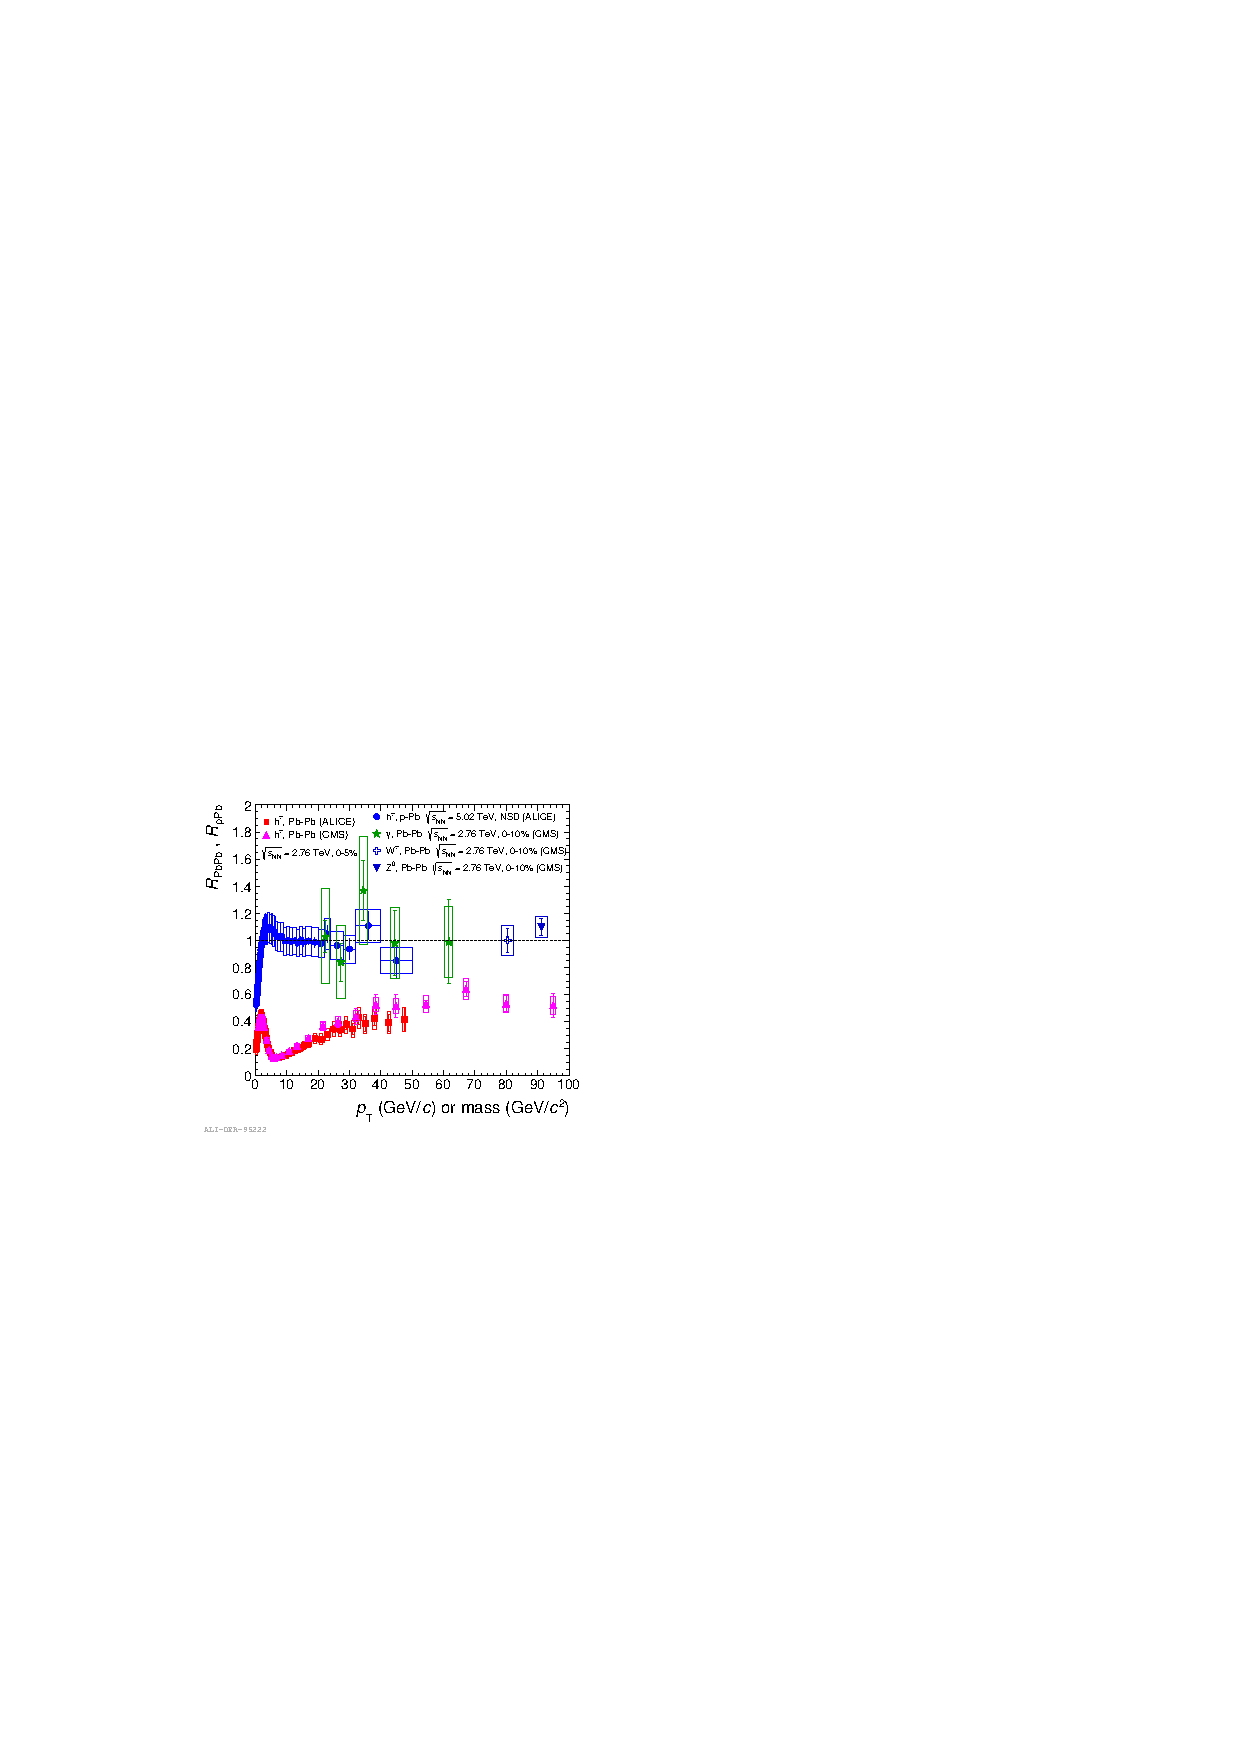
\includegraphics[width=0.8\textwidth]{Introduction/alice_hadron_raa.pdf}
    \caption{Comparisons of $R_\mathrm{PbPb}$ and $R_\mathrm{pPb}$ for various single particles measured by ALICE and CMS \cite{Bencedi2016}.}
    \label{fig:raa_particles}
  \end{figure}


  % ThisisonereasonthatRAA for hadrons rises at the highest pT even though RAA for jets remains comparably suppressed

\subsection{Flow in Small Systems}

It should be noted, however, that flow -- a key signature of a viscous fluid -- is not exclusive to AA collisions. Non-zero measurements of flow have been observed in high multiplicity pp collisions at CMS \cite{Khachatryan2010} in p--Pb collisions at ALICE and LHCb \cite{Abelev2013,Aaij2016}, and in $p/d/^3$He +Au collisions at PHENIX \cite{PHENIXCollaboration2018}. Figure~\ref{fig:near_side_ridge} shows the famous "near side ridge" in high centrality p--Pb, a feature most likely attributable to the hydrodynamic evolution of the initial collision geometry (closely related to $v_2$).

\begin{figure}[htpb]
  \centering
  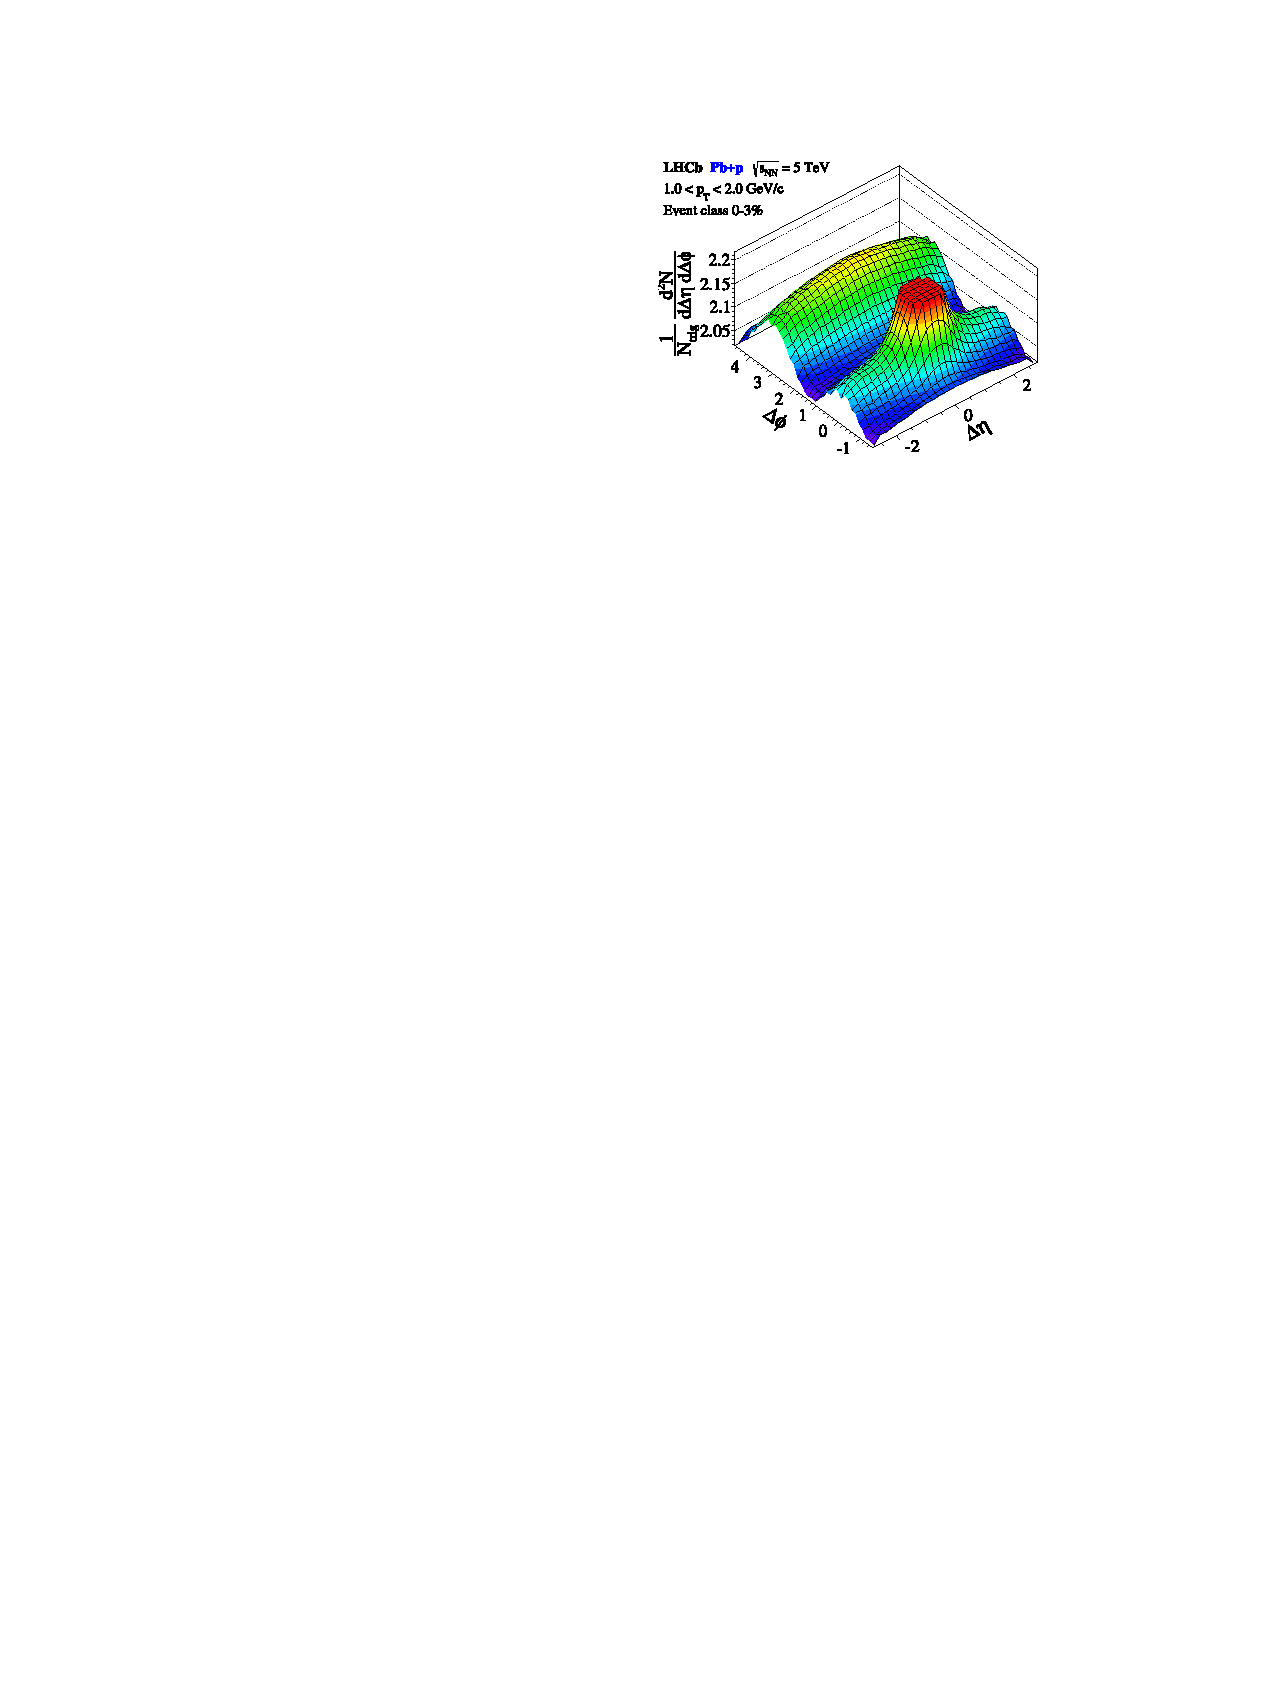
\includegraphics[width=0.8\textwidth]{Introduction/near_side_ridge.pdf}
  \caption{Two-particle correlation for high-event activity in p–Pb collisions at 5.02 TeV measured with the LHCb detector \cite{Aaij2016}.}
  \label{fig:near_side_ridge}
\end{figure}

 The ``near-side ridge'' observed here is often thought to be the result of collectivity or flow, hinting that there there may be some hydrodynamic behavior even in these small systems. The degree of hydrodynamic behavior can be quantified by $v_2$, as mentioned before, and is shown in Fig.~\ref{fig:small_systems_v2}, where a non-zero  $v_2$ in pp, and p--Pb (as well as PbPb) is shown: the ridge at larger \deltaphi is attributed to jets produced in the collision. In the simple 2-2 scattering picture in which the initial total \pt is 0, the two scattered partons should be back-to-back in \deltaphi~to conserve momentum, and so a jet peak is expected at larger \deltaphi. However, the partons in the initial system  do not necessarily have 0 \pt. Both partons can have an initial transverse momentum, \kt, that makes up a component of their overall momentum fraction of the nucleon. Differences in \kt between the colliding partons result in a larger spread of the jet peak along $\Delta\eta$. This is known as \kt~smearing \cite{PHENIXCollaboration2006}, and the effect is a long prominent ridge along  $\Delta\eta$ centered at approximately \deltaphi$\approx \pi$.
% Fig. \ref{fig:small_systems_v2} shows the measured, non-zero $v_2$  in pp, p--Pb and PbPb. 
\begin{figure}[htpb]
  \centering
  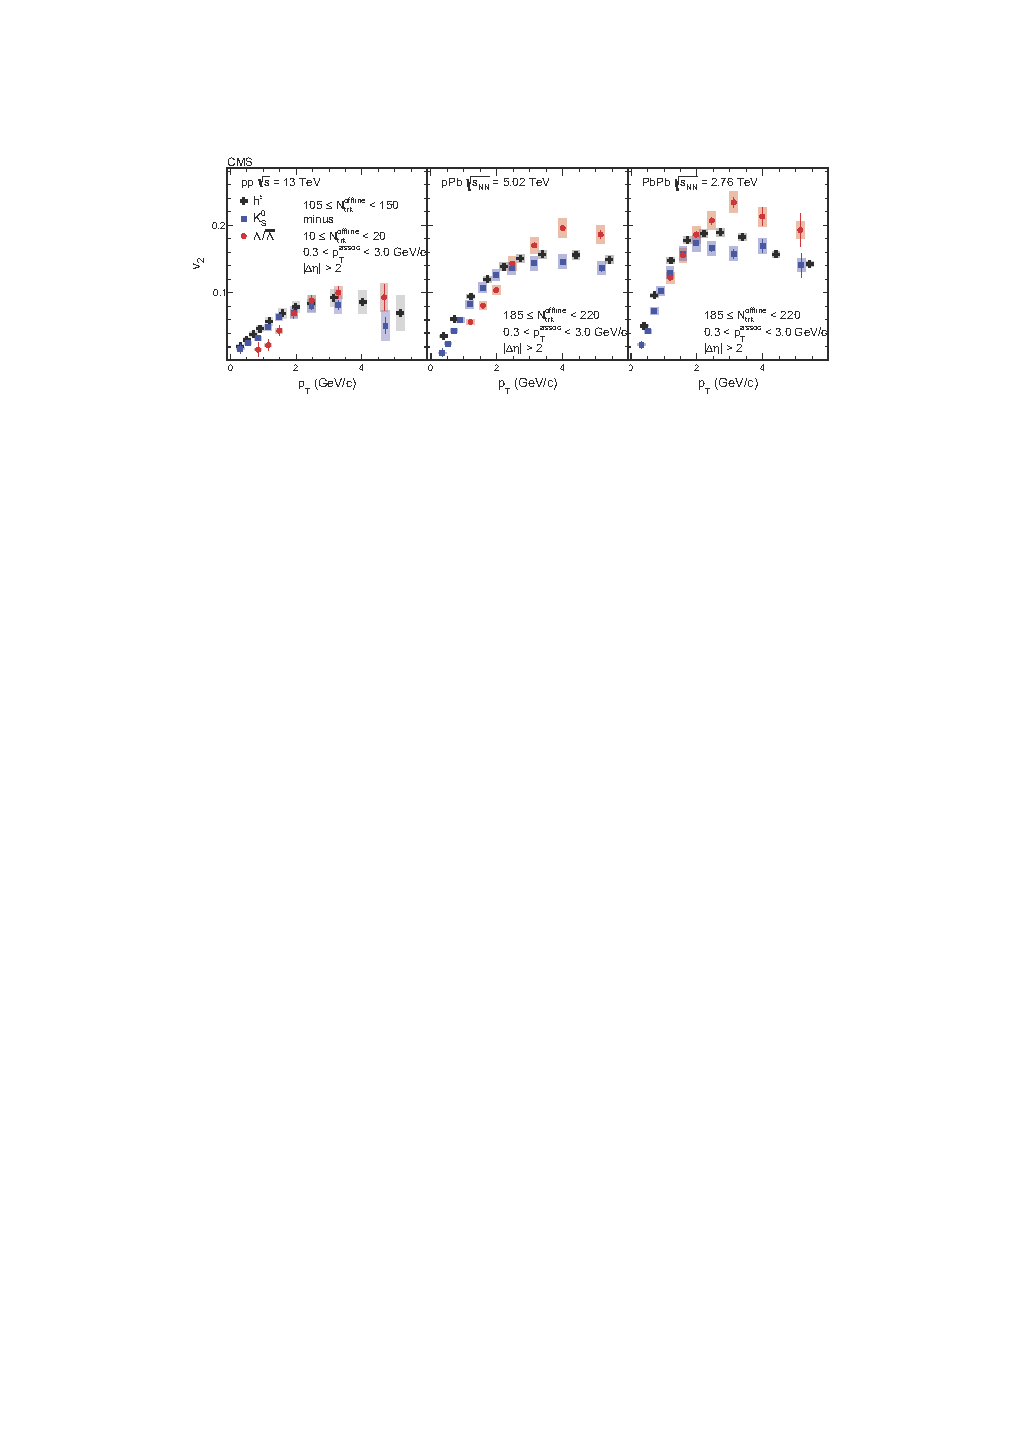
\includegraphics[width=0.99\textwidth]{Introduction/small_systems_flow.pdf}
  \caption{The $v_2$ data measured in pp, pPb and PbPb collisions by CMS as a function of $p_\mathrm{T}$ for charged particles, $K_0^s$ and $\Lambda$ particles at high multiplicities from two-particle correlations \cite{Khachatryan2017,Khachatryan2015}.}
  \label{fig:small_systems_v2}
\end{figure}

These observations came as quite the surprise: these smaller systems were previously thought to have insufficient energy density for deconfinement to occur and contained too few particles in the collision for thermalization and the equations of hydrodynamics to meaningfully apply.

% The observation of the near side ridge as  well as non-zero $v_2$ (both observed in pp and p--Pb) has called into question the assumption that QGP is not produced in these smaller systems. Additionally, the case of pp is particularly interesting, as the number of particles was also thought to be too small to meaningfully reach a state of thermalization, nor to be reasonably described by hydrodynamics. This has spawned quite interesting work on the applicability of hydrodynamics in systems far from equilibrium \cite{Romatschke2018a}.

The observation of flow, however, is not a sufficient condition to for claiming the creation of quark gluon plasma. One hypothesis claims that this phenomenon is not solely attributable to the formation of QGP. There has been quite interesting work on the applicability of hydrodynamics in systems far from equilibrium \cite{Romatschke2018a}, and findings that indicate that measurements of $v_n$ do not necessarily imply equilibrium \cite{Romatschke2017}. But the question of why hydrodynamics describes these small systems so well \cite{Habich2016, Zhao2018a} remains an open question in the field. On the other hand, another hypothesis is that a tiny droplet of QGP is formed in these smaller systems. While our current understanding of the conditions required for the formation of QGP indicates that it may in fact be possible to create a QGP in these systems, this is troubling for other reasons. These smaller systems often serve a "control" for quantifying the modifications observed in AA collisions that are attributed to QGP. This all points to the increased necessity of measuring modifications in smaller systems, particularly attempting to disentangle the effects of hot nuclear matter from cold nuclear matter, and is a principle focus of this thesis.

As stated previously, the presence of flow effects in small systems has not unambiguously stipulated the creation of a quark gluon plasma in these systems.  Other observables such as the broadening of the away side correlation need to be studied. In particular, however, a "smoking gun" of QGP production, discussed in the next section, has yet to be observed in small systems, despite an extensive search for it.


\section{Fragmentation Functions}
\label{sec:FF}
One of the simplest ways to study QCD is to measure hadron production in $e^+ + e^-$ collisions, particularly through the process  $e^+ + e^- \rightarrow q\bar{q}$. The inclusive cross section for hadron production ($\sigma$) may be written as the product of the partonic cross section ($\hat{\sigma}$) and a parametrization of the non-calculable long-range behavior called the fragmentation function (FF), denoted $D_c^h(z)$ is the probability for a parton of flavor $c$ to fragment into a hadron taking a fraction $z=p_h/p_c$ of its momentum:

  \begin{equation}
    d\sigma = \sum_c\int dz d\hat{\sigma}(p_a,p_b,p_c)D_c^h(z)
    \label{eq:hadron_cross_section}
  \end{equation}

  This property is known as factorization. It is an approximation that does not always hold, though it has only been explicitly proven in a limited number of cases \cite{Collins1989}. Experimentally, the yield of hadrons as a function of $z$ associated with a parton (or jet) of known momentum is a measure of the fragmentation function. Experimentally, an alternative variable, $\zt=\pt^h/\pt^\mathrm{trig}$, is often used where $\pt^{trig}$ is the transverse moment of a jet, or other object related to a hard scattered parton. 

A more complex but relevant observable is the semi-inclusive cross section in Deep Inelastic Scattering (SIDIS). In electron-proton collisions, semi-inclusive scattering simply indicates that not all the particles are measured. In e+p collisions, semi-inclusive scattering measures at least one other hadron in coincidence with the scattered electron. \textit{Exclusive} scattering, indicates that \textit{all} particles produced in the collision are measured. These definitions appear counter-intuitive, at least in terms of what's measured in the collision. But the distinction comes from the underlying physical processes that each measurement corresponds to. In semi-inclusive scattering, there are often several physical processes that could have resulted in the limited number of measured particles. For example, there are a variety of processes that give rise to a $q\bar{q}$ pair, all of which must be considered in an event where exactly two jets are measured in coincidence with the scattered electron. In exclusive scattering, because all particles are measured in the collision, the underlying physical process producing those particles is much  more readily identified, to the exclusion of other potential processes. Unlike e+p collisions, in heavy ion collisions the shear number of particles produced, a substantial fraction of which are neutral particles that are notoriously difficult to measure, exclusive measurements are essentially impossible. The term Deep Inelastic is more straightforward; rather than an elastic collision where momentum is conserved, much of the energy goes towards breaking up the proton(Ion). The semi-inclusive DIS cross section can be written as:

  \begin{equation}
    d\sigma= \sum_{a,c} \int dx_a dz f_a(x_a) d\hat{\sigma}(p_a,p_b,p_c) D_c^h(z).
    \label{sidis_cross_section}
  \end{equation}
where (Bjorken) \textit{x} is the fraction of the proton’s momentum carried by the parton, and $f_x(x)$ is the parton distribution function (PDF) that describes the partons in their initial state before the collision. At first glance, this equation is troubling, as it appears that a careful measurement of the hadronic cross section cannot uniquely determine the PDF or fragmentation function. The long-range behavior of these fragmentation functions, however, is thought to be independent of the collision process, a property known as \textit{universality}. Thus, the same fragmentation functions are thought to apply regardless of the particle species being collided. On the other hand, parton distribution function is only a property of the objects being collided and can be factorized from the collision process and subsequent fragmentation. 
 
  The cross section for hadro-production in proton-proton collisions can be expressed in a similar way with the addition of a second integral over the additional parton:

  \begin{equation}
    d\sigma= \sum_{a,c} \int dx_a dx_b dz f_a(x_a) f_b(x_b) d\hat{\sigma}(p_a,p_b,p_c) D_c^h(z).
    \label{p+p_sidis}
  \end{equation}

  This gives rise to an interesting picture of progression, albeit a slightly oversimplified one: fragmentation functions are measured in $e^+ + e^-$ collisions, shown in Fig.~\ref{fig:pdg_ff}, which are then used in DIS data. Then, the DIS data is used to determine the PDF's, shown in Fig.~\ref{fig:dis_pdfs} which are applied to $p+p$ collisions.

  \begin{figure}[htpb]
    \centering
    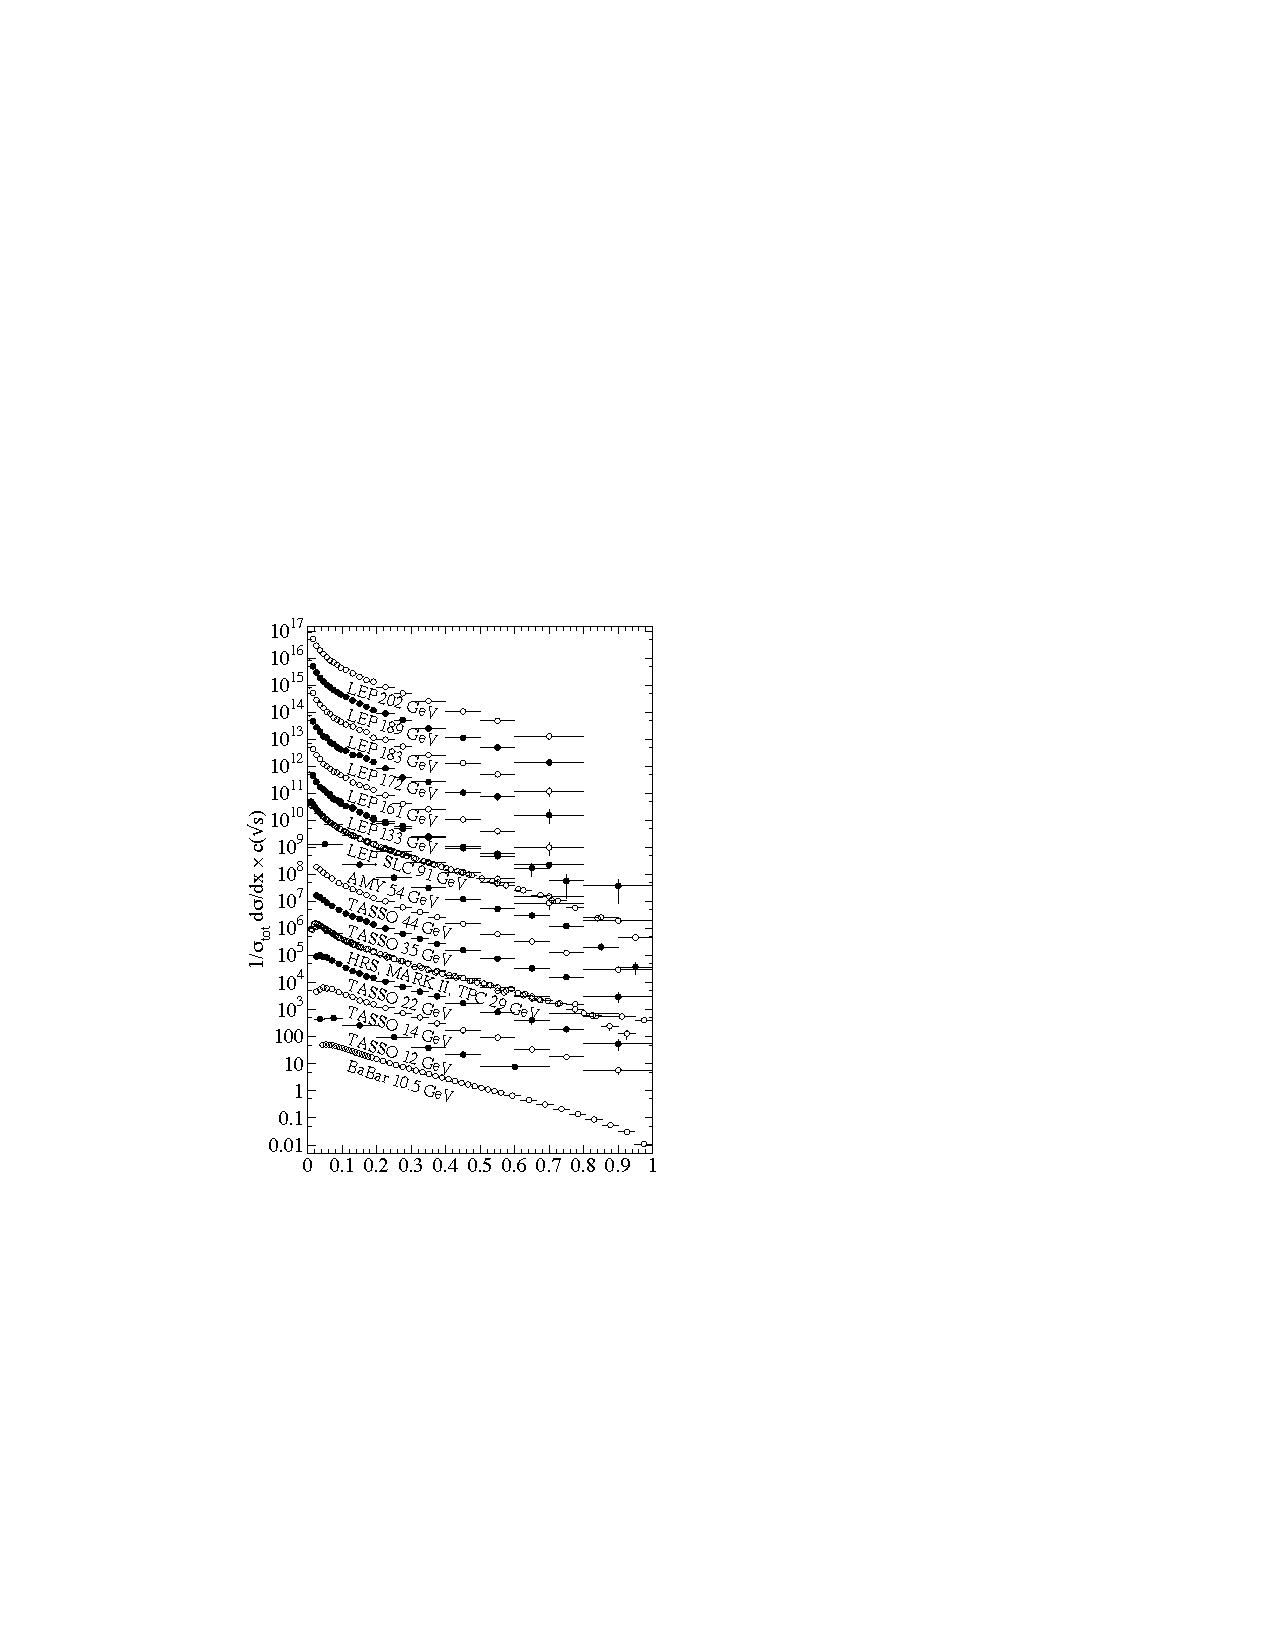
\includegraphics[width=0.8\textwidth]{Introduction/pdg_ff.pdf}
    \caption{The $e^+e^-$ fragmentation function for all charged particles for different CM energies  $ \sqrt{s} $ versus $x$. For the purpose of plotting, the distributions were scaled by  $c(\sqrt{s}) = 10^i$, where $i$ ranges from i=0 ($\sqrt{s}=12$ GeV) to i=13 ($\sqrt{s} = 202 $ GeV) \cite{deFlorian2018}} 
    \label{fig:pdg_ff}
  \end{figure}
  
  \begin{figure}[htpb]
    \centering
    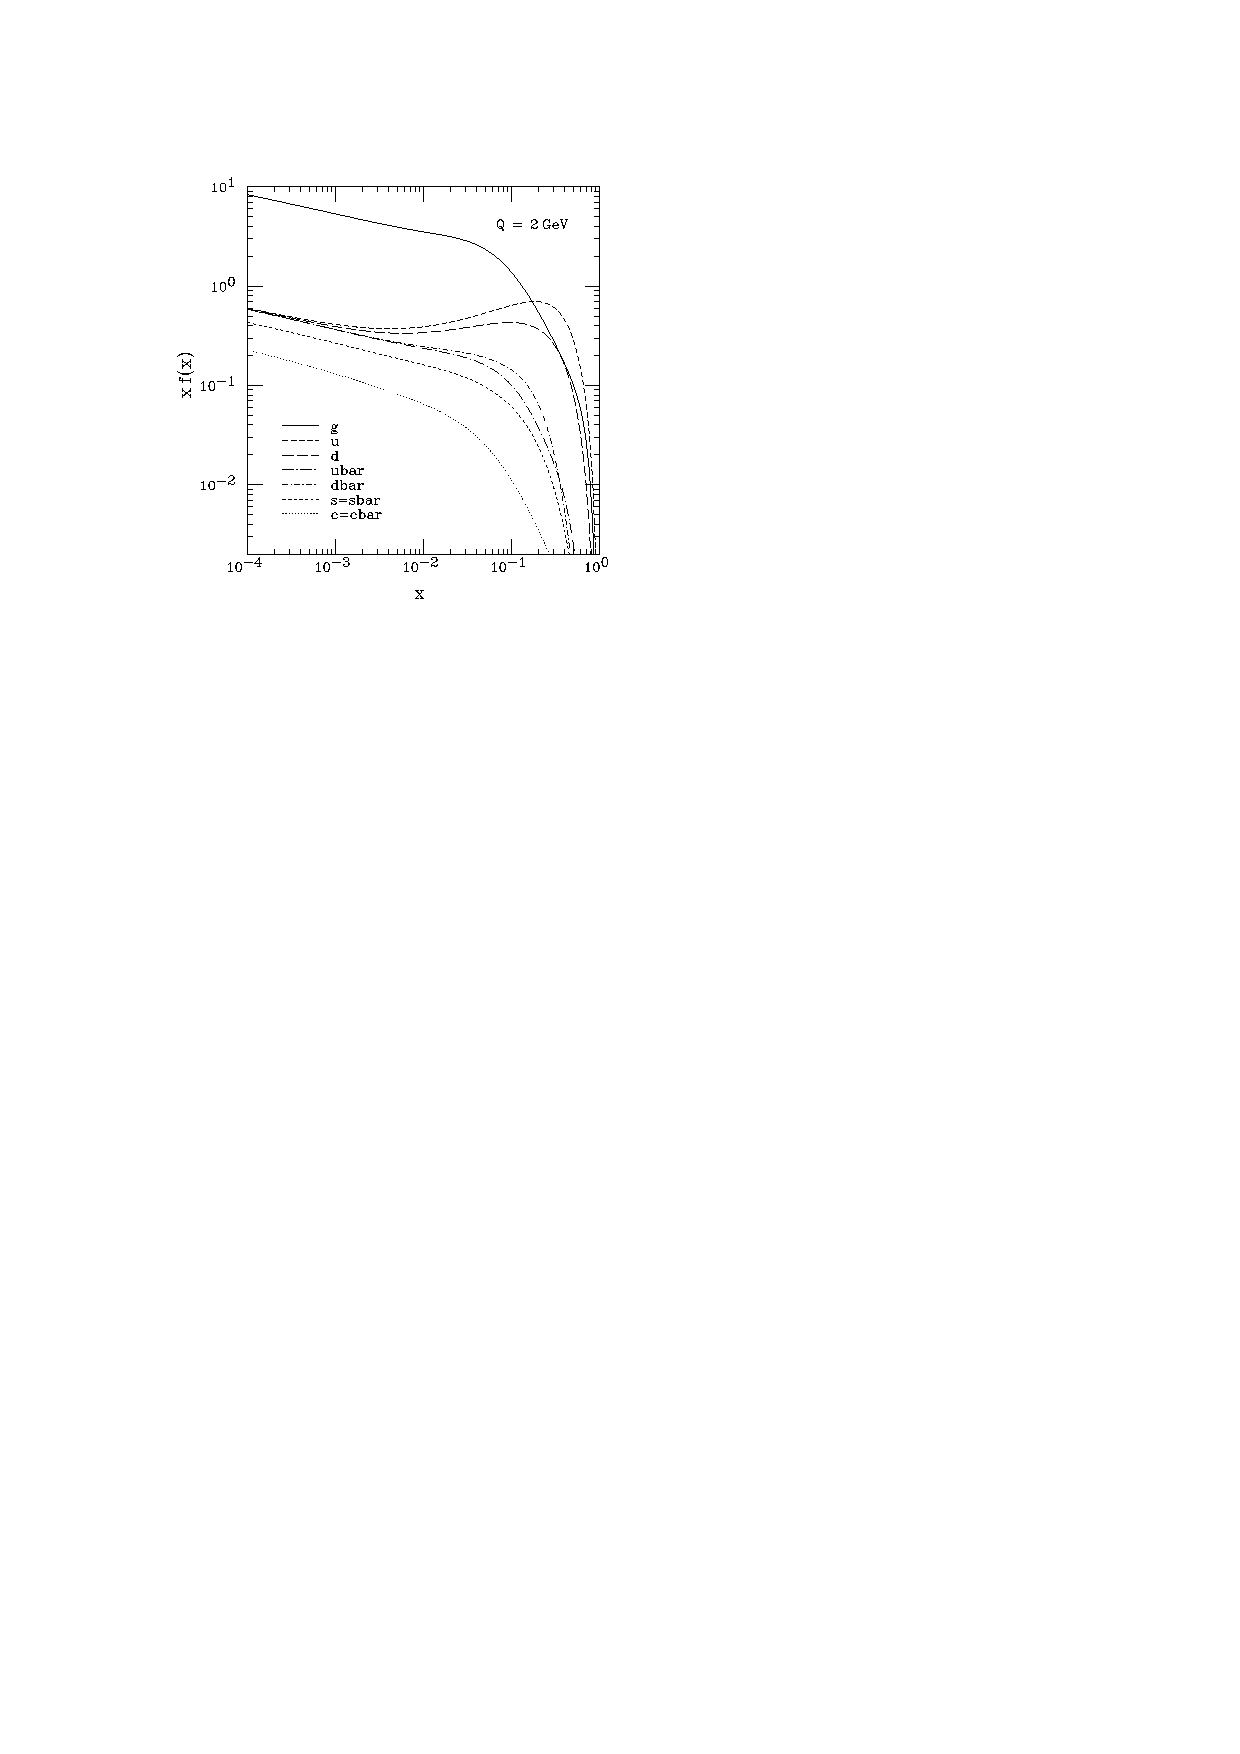
\includegraphics[width=0.8\textwidth]{Introduction/pdfs.pdf}
    \caption{Sampling of PDFs from CTEQ \cite{Pumplin2002}}
    \label{fig:dis_pdfs}
  \end{figure}

In a similar story of progression, p+p collisions are important baseline data for collisions of heavy nuclei, discussed in Sec.~\ref{sec:raa}. It turns out, expectations for hadronic observables must be modified in nuclear collisions. Furthermore, p+Pb collisions are important for disentangling cold and hot nuclear matter effects. Such departures provide a window into physics beyond the vacuum behavior of QCD accessed via elementary particles collisions. 


% \section{Cold Nuclear Matter Effects}\label{sec:coldnm}
% shadowing, kT effect, others\ldots.


\section{Two Particle Correlations}
Another way to study energy loss effects on partons propagating through a medium in heavy ion collisions is by measuring two particle correlations. One of simplest forms of two particle correlations is the di-hadron correlation. Contemporary jet measurements invoke jet reconstruction algorithms to determine the full energy of the jet event-by-event. These methods are difficult to apply in heavy-ion collisions due to the overwhelming background from soft particles, and may be less sensitive to medium modification depending on the observable being measured. Instead, a very useful approach has been to measure correlations between particles.

\begin{equation}
    Y(\deltaphi)\equiv \frac{1}{n^\mathrm{triggers}}\frac{\mathrm{d}N}{\mathrm{d}\deltaphi}
    \label{eq:yield}
  \end{equation}
where $N$ is the number number of correlated particles, $n^\mathrm{triggers}$ is the measured number of triggers \footnote{A trigger is generally a condition required to be met in order to record the event data. For two-particle correlations, it is often a high-\pt hadron, jet, or photon.}, and $\deltaphi$ is the difference in azimuthal angle between the trigger and associated particle. Figure~\ref{fig:dihadron_cartoon} shows a simplified example of a di-hadron (hadron-hadron, or h-h) correlation in p+p collisions. The two-peak structure is characteristic of such measurements, and indicates that the event sample is dominated by di-jet events. The particles within the same jet make up the narrow peak centered around \deltaphi~= 0 and the recoil jet appears as the peak around $\deltaphi = \pi$. The away side peak is broadened since kinematically the away side jet can swing along the $\eta$ direction and $k_\mathrm{T}$, the initial pair momentum of the colliding partons, can create an imbalance in the jets’ energy and cause them to be acoplanar. $\eta$, also referred to as pseudorapidity, is defined as $\eta = \ln(\tan(\theta/2))$, where $\theta$ is the polar angle with respect to beam direction. A 2D plot ($\deltaphi,\Delta\eta$) of this correlation in pPb and pp collisions is shown in Fig.~\ref{fig:near_side_ridge}, Sec.~\ref{sec:flow}. The peaks sit atop a pedestal which is due to initial and final state interactions amongst the beam remnants and the hard-scattered partons. This must be subtracted, and will be discussed in greater detail in Sec.~\ref{sec:ue_subtraction} for pp and pPb collisions. For AA collisions, this subtraction is even more complicated, where flow is no longer a signal, but a background phenomenon that must also be subtracted in correlation analyses. 

  \begin{figure}[htpb]
    \centering
    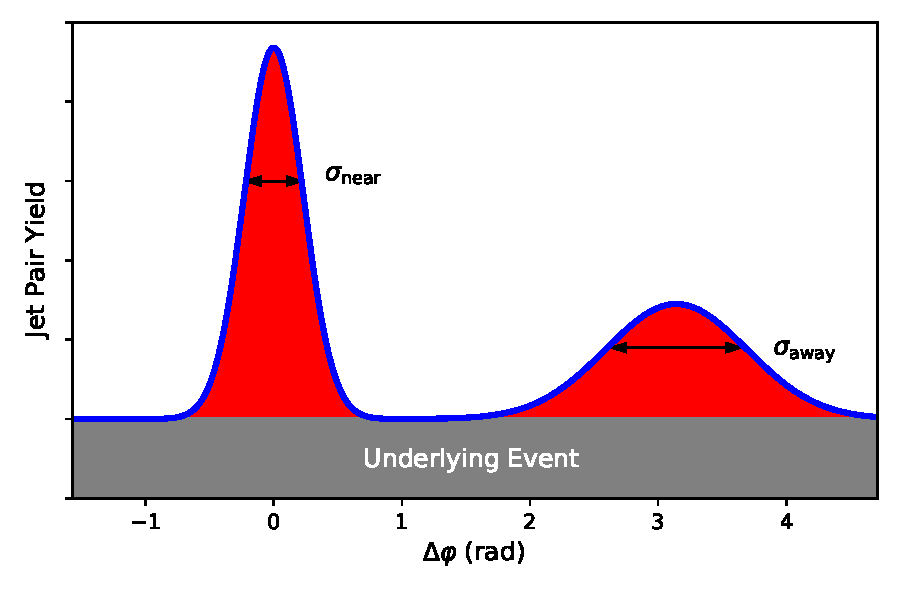
\includegraphics[width=0.8\textwidth]{Introduction/dihadron_cartoon.pdf}
    \caption{Cartoon illustrating a measurement of two-particle correlations from jets}
    \label{fig:dihadron_cartoon}
  \end{figure}

  The STAR experiment performed a hadron-hadron correlation measurement with triggers of $p_{\mathrm{T},t}>$ 4 GeV/$c$ and associated partners of 2 GeV$/c<p_{\mathrm{T},a}<p_{\mathrm{T},t}$. The result, shown in Fig.~\ref{fig:dihadron_correlation} demonstrates that for central Au + Au collisions the near-side jet looks very similar to p+p but the away-side jet completely disappears. This is consistent with a picture in which the near-side jet is usually produced near the surface and the away-side jet is completely absorbed by the medium.

  \begin{figure}[htpb]
    \centering
    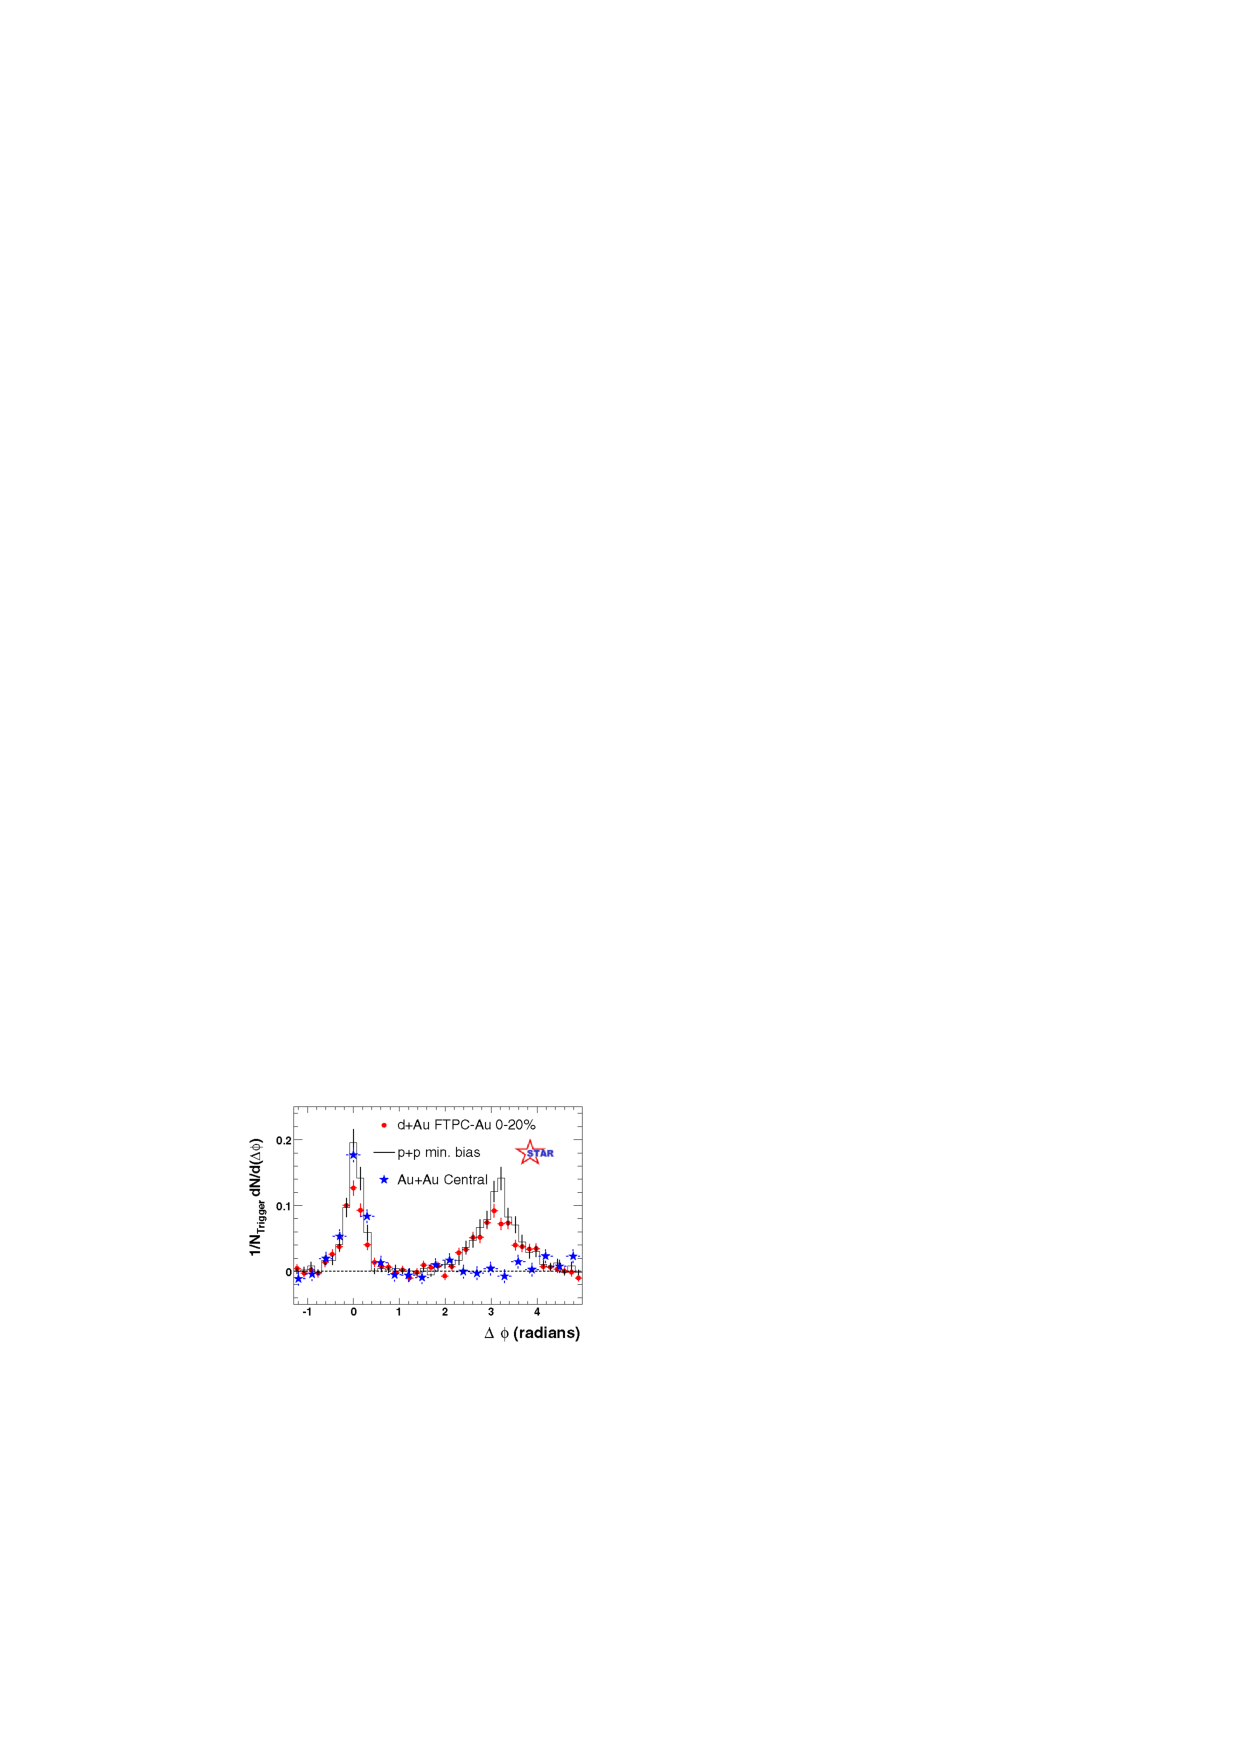
\includegraphics[width=0.8\textwidth]{Introduction/star_dihadron.pdf}
    \caption{Hadron-hadron correlations measured in p+p, d+Au and Au+Au collisions at STAR. The near side jet peaks around $\deltaphi$=0 in all three systems but the away-side which peaks around $\deltaphi=\pi$ in p+p and d+Au, is suppressed in Au+Au \cite{Adams2005}.}
    \label{fig:dihadron_correlation}
  \end{figure}

Although hadron-hadron correlations have revealed a great deal about energy loss in the medium, they are limited by the fact that the initial parton momentum is unknown and cannot be used to directly measure the fragmentation function.

\section{Prompt Photons}
\label{sec:prompt}
Prompt photons can be defined simply as the photons produced immediately in the collision, before final state hadrons are produced. At the lowest order in pQCD, prompt photons are produced via two processes: (i) quark-gluon Compton scattering, $qg \to q\gamma$, (ii) quark-antiquark annihilation, $q\overline{q} \to g\gamma$, and, with a much smaller contribution,  $q\overline{q}\to$ $\gamma\gamma$. In p+p collisions, the Compton-type process dominates the cross section by roughly an order of magnitude over annihilation as a result of the scarcity of antiquarks. Additionally, prompt photons can be produced in higher-order processes, such as fragmentation or bremsstrahlung \cite{Aurenche1993}. The collinear part of such processes has been shown to contribute effectively also at lowest order. The basic Feynman diagrams for these processes (excluding $q\overline{q}\to$ $\gamma\gamma$) are shown in Fig.~\ref{fig:prompt_feynman}.

\begin{figure}[htpb]
  \centering
  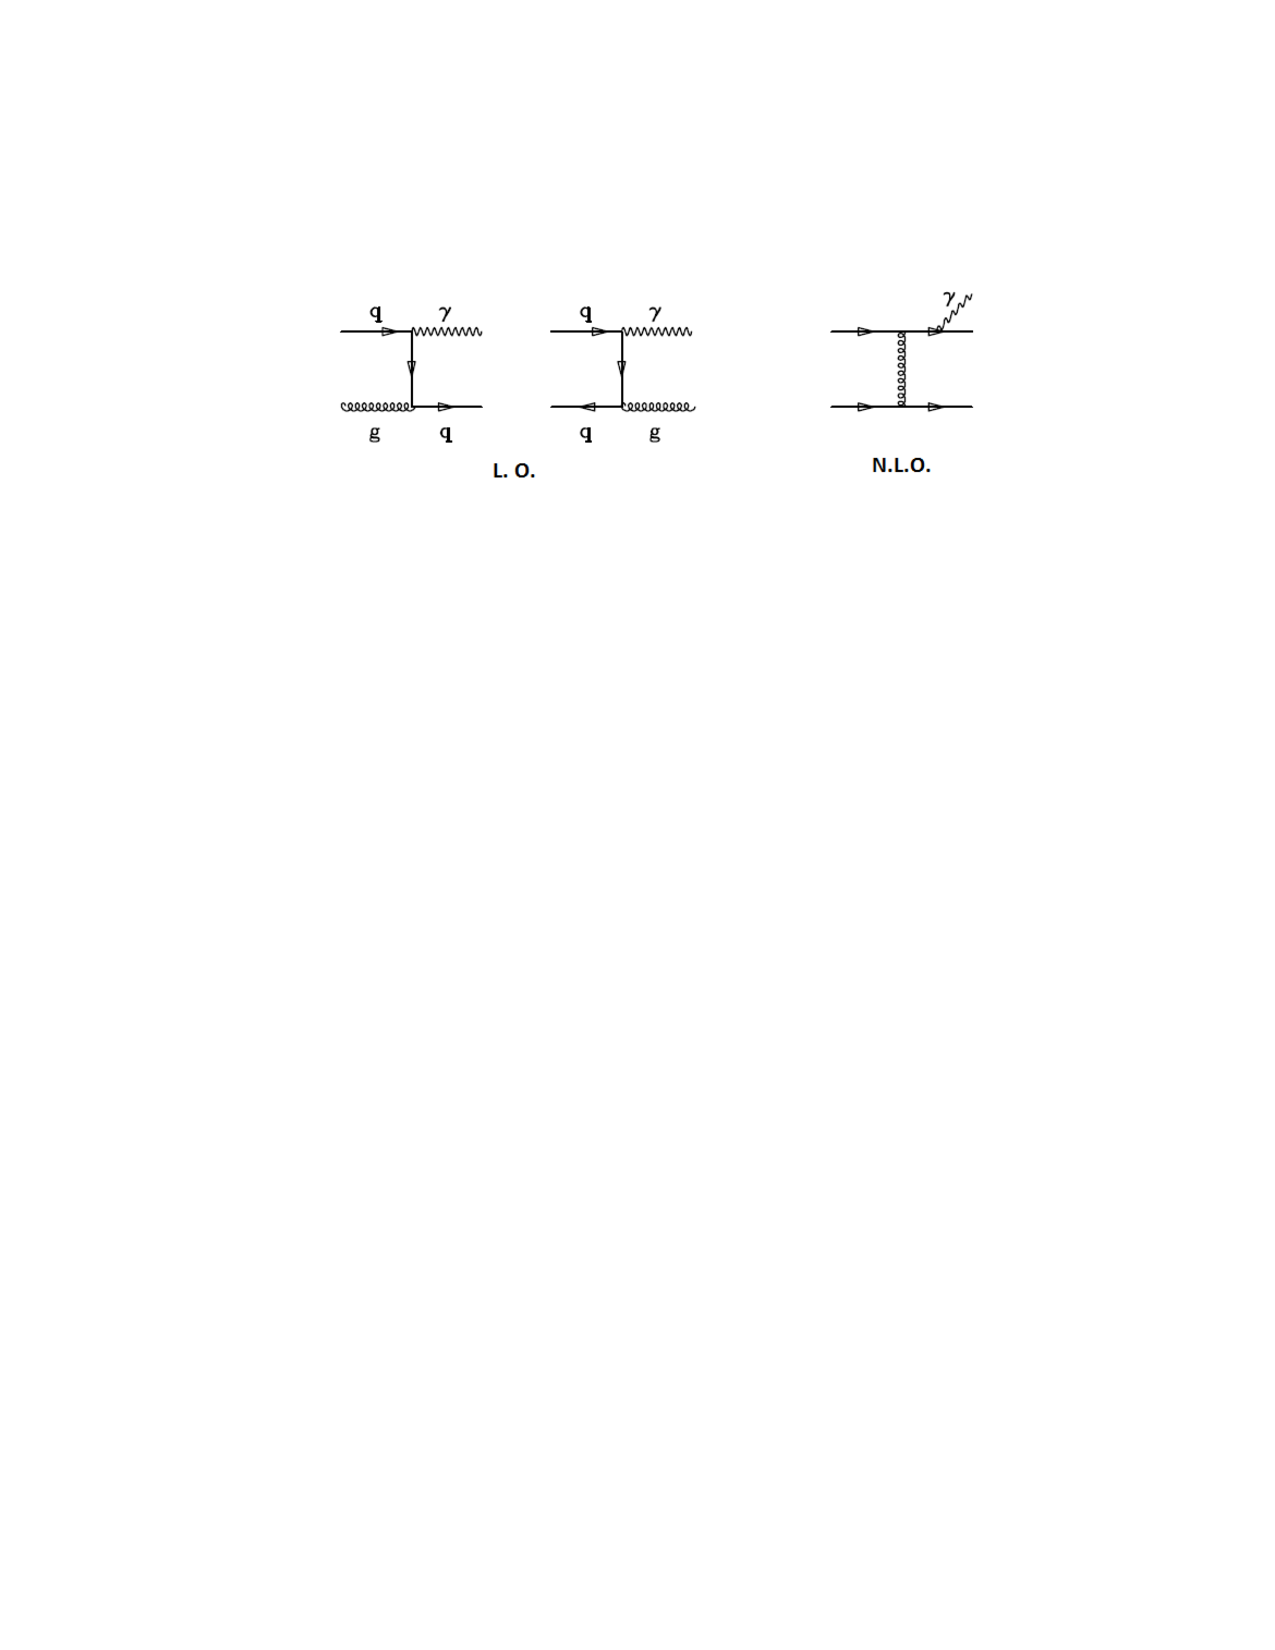
\includegraphics[width=0.8\textwidth]{Introduction/prompt_photons.pdf}
  \caption{On the left are the leading order Feynman diagrams for direct photon production. The diagram on the right is next-to-leading order. Photons resulting from this diagram are referred to as fragmentation photons.}
  \label{fig:prompt_feynman}
\end{figure}

%ALICE-Prompt: Photons not from hadronic decays
%PHENIX-Prompt: RIGHT FROM THE COLLISION (excludes fragmentation)
%Direct is the same in both cases.
%%%%%LEADING ORDER FEYNMAN DIAGRAMS FROM QUAL%%%%%%%%%

Photons produced during fragmentation, are aptly named fragmentation photons. As a result, fragmentation photons are often surrounded by a larger amount of energy and hadronic activity than other prompt photons produced from the initial hard scattering.

Prompt photons, and by extension fragmentation photons, are both included in the definition of direct photons. While the definition of direct photons is not always consistent in the literature, and varies slightly between experiments, we define direct here to mean any photon not produced from hadronic decays. Those photons originating from the decay of a hadronic bound state are defined as decay photons. The two largest sources of decay photons are the two-photon decay channels of the $\pizero$ and $\eta$ meson. At higher \pt, decay photons make up the majority of photons produced in the collision.

Together, direct and decay photons make up all the photons observed in a collision, called inclusive photons.

\begin{equation}
  \gamma_\mathrm{inclusive} = \gamma_\mathrm{direct} + \gamma_\mathrm{decay}
\end{equation}

\section{Photons in Heavy Ion Collisions}
Direct photons have three very important properties that make them valuable tools in heavy-ion physics. First, there are relatively few leading order diagrams which contribute to direct photon production. Second, the photon-quark coupling is point-like, and not affected by long-range QCD behavior such as fragmentation in the final state. Third, though a property shared with other high-\pt~photons, they do not interact with the QGP. Prompt photons are thus extremely valuable tools in heavy-ion physics. 

One property that makes them so useful is that they are not expected to interact with the QGP. Photons do not carry color charge, and should therefore be unmodified by strong interactions in a medium, while the plasma is made up of quarks that carry (fractional) charge, For example, the mean free path of a 1 GeV photon in a QGP at $T=$200 MeV was calculated to be  $\lambda=480$ fm, much larger than the estimate size of plasma at  $r \approx 10$ fm~\cite{David2020}. Thus, in the leading order picture, after prompt photons are produced early in the collision they should propagate through the medium completely unmodified, with no high \pt~suppression. This has been verified, by measuring the $R_\mathrm{AA}$ of photons, shown in Fig.~\ref{fig:photon_raa}. A measured $R_\mathrm{AA}$ consistent with 1.0 strongly supports the position that photons are unmodified in the quark gluon plasma.

\begin{figure}[htpb]
  \centering
  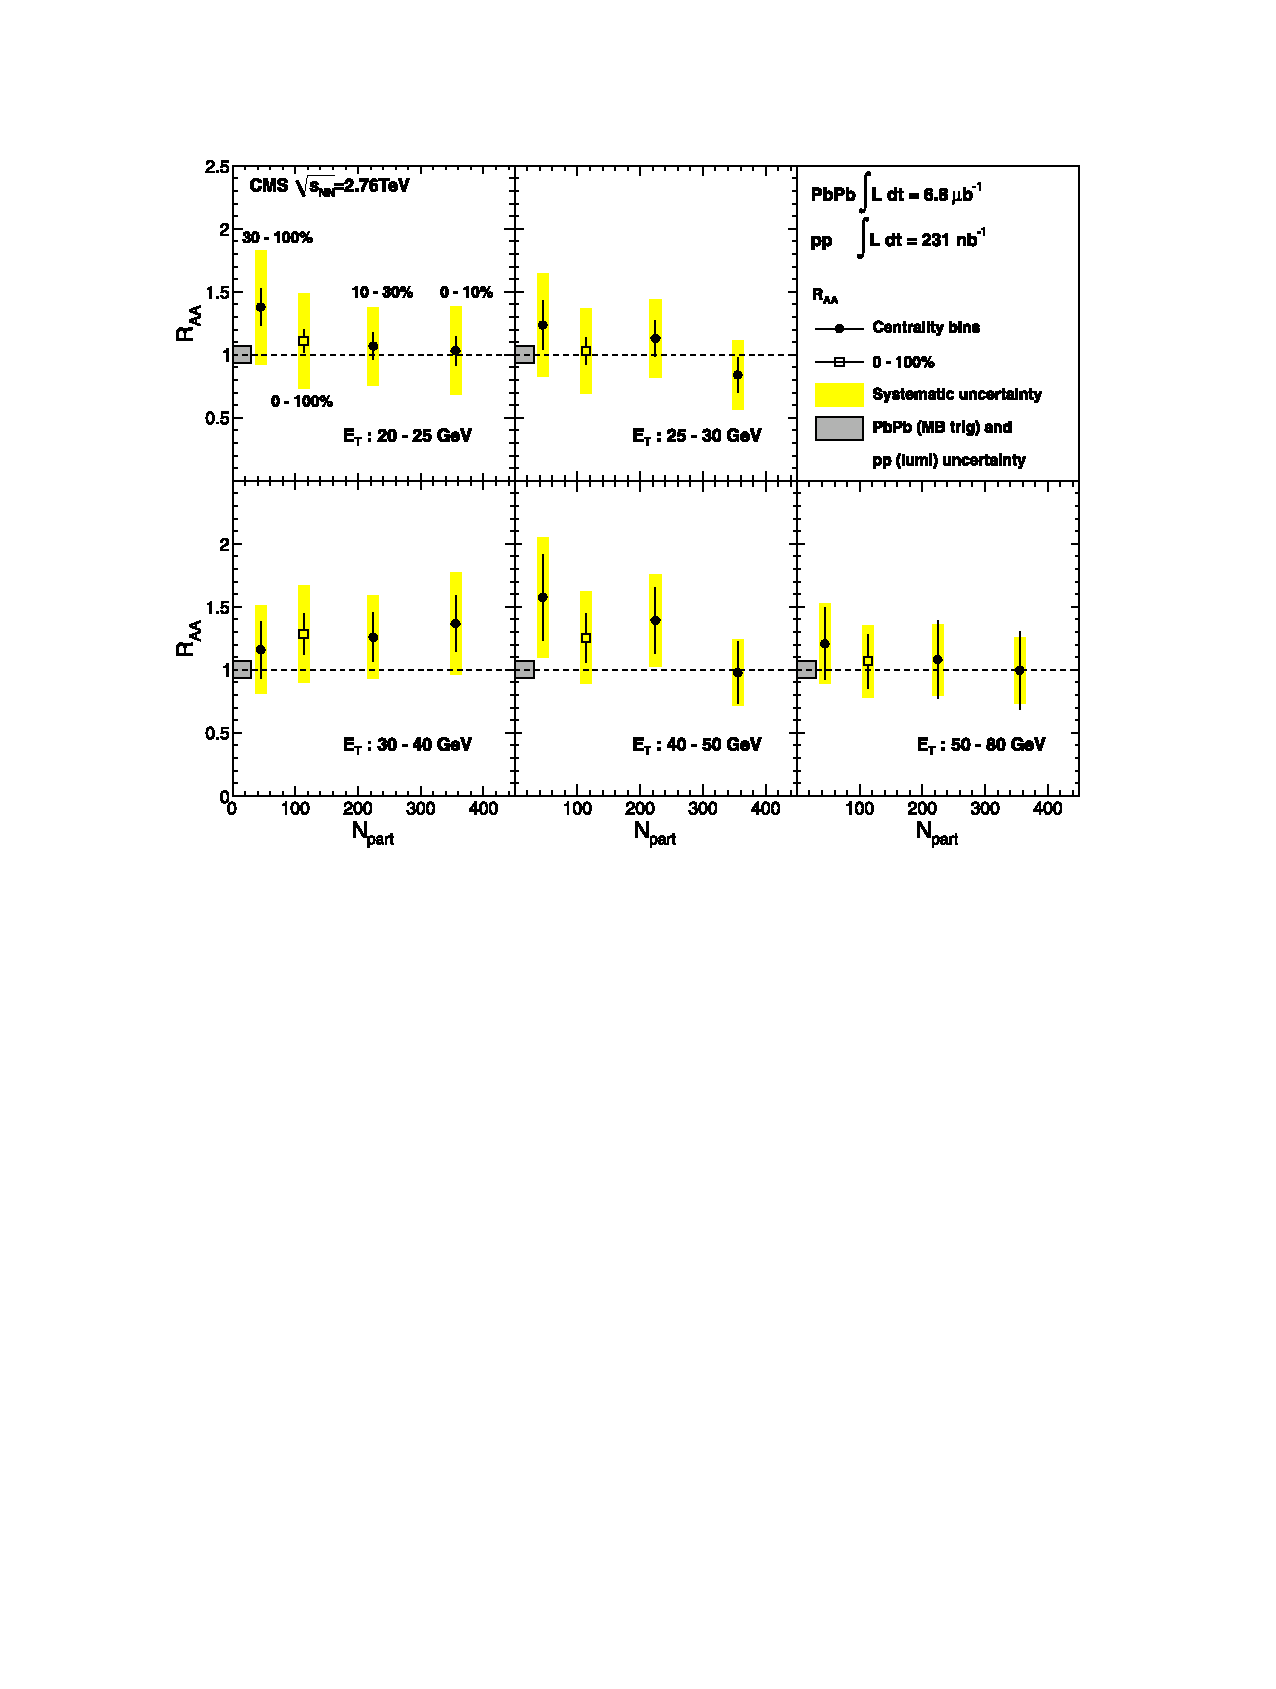
\includegraphics[width=0.8\textwidth]{Introduction/photon_raa}
  \caption{The measured nuclear modification factor $R_\mathrm{AA}$ for photons as a function of PbPb centrality (given by the number of participating nucleons,$N_\mathrm{part}$) for five different photon transverse energy ($E_\mathrm{T}$) intervals \cite{Chatrchyan2012}.}
  \label{fig:photon_raa}
\end{figure}


% For γ − h correlations, on the other hand, the conditional yield should be much more closely related to the fragmentation function. In the leading order picture, the direct photon exactly balances the away-side jet and therefore, the measurable quantity, pT,a/pT,t, is nothing but the fragmentation variable pT,a/pT,jet. This explains why γ − h correlations are a powerful measurement. They provide a source of recoil partons of fixed momentum. Their conditional yields in p + p collisions only probe the jet fragmentation. By contrast, hadron correlations are controlled by the jet cross section which also depend on the PDF’s and the parton scattering cross sections.

\subsection{$\gamma$-Jet Correlations}
\label{sec:intro_gj}
Another important property of leading order prompt photons is that the photon-quark coupling is point-like and therefore not complicated by long-range QCD behavior such as jet fragmentation in the final state, unlike hadronic observables. Thus, in the leading order picture, the direct photon exactly balances the away-side parton and resulting jet. Here the photon acts as a reference for the parton from the initial scattering, before any modification in heavy-ion collisons. This means that comparisons between the photon and parton, or jet, as well as large deviations from \deltaphi~$\approx\pi$ can be used to directly study medium-induced effects on the recoiling parton. $\gamma$-jet correlations in CMS are shown in Fig.~\ref{fig:cms_gj_correlations}~\cite{Sirunyan2018}.


\begin{figure}[htpb]
  \centering
  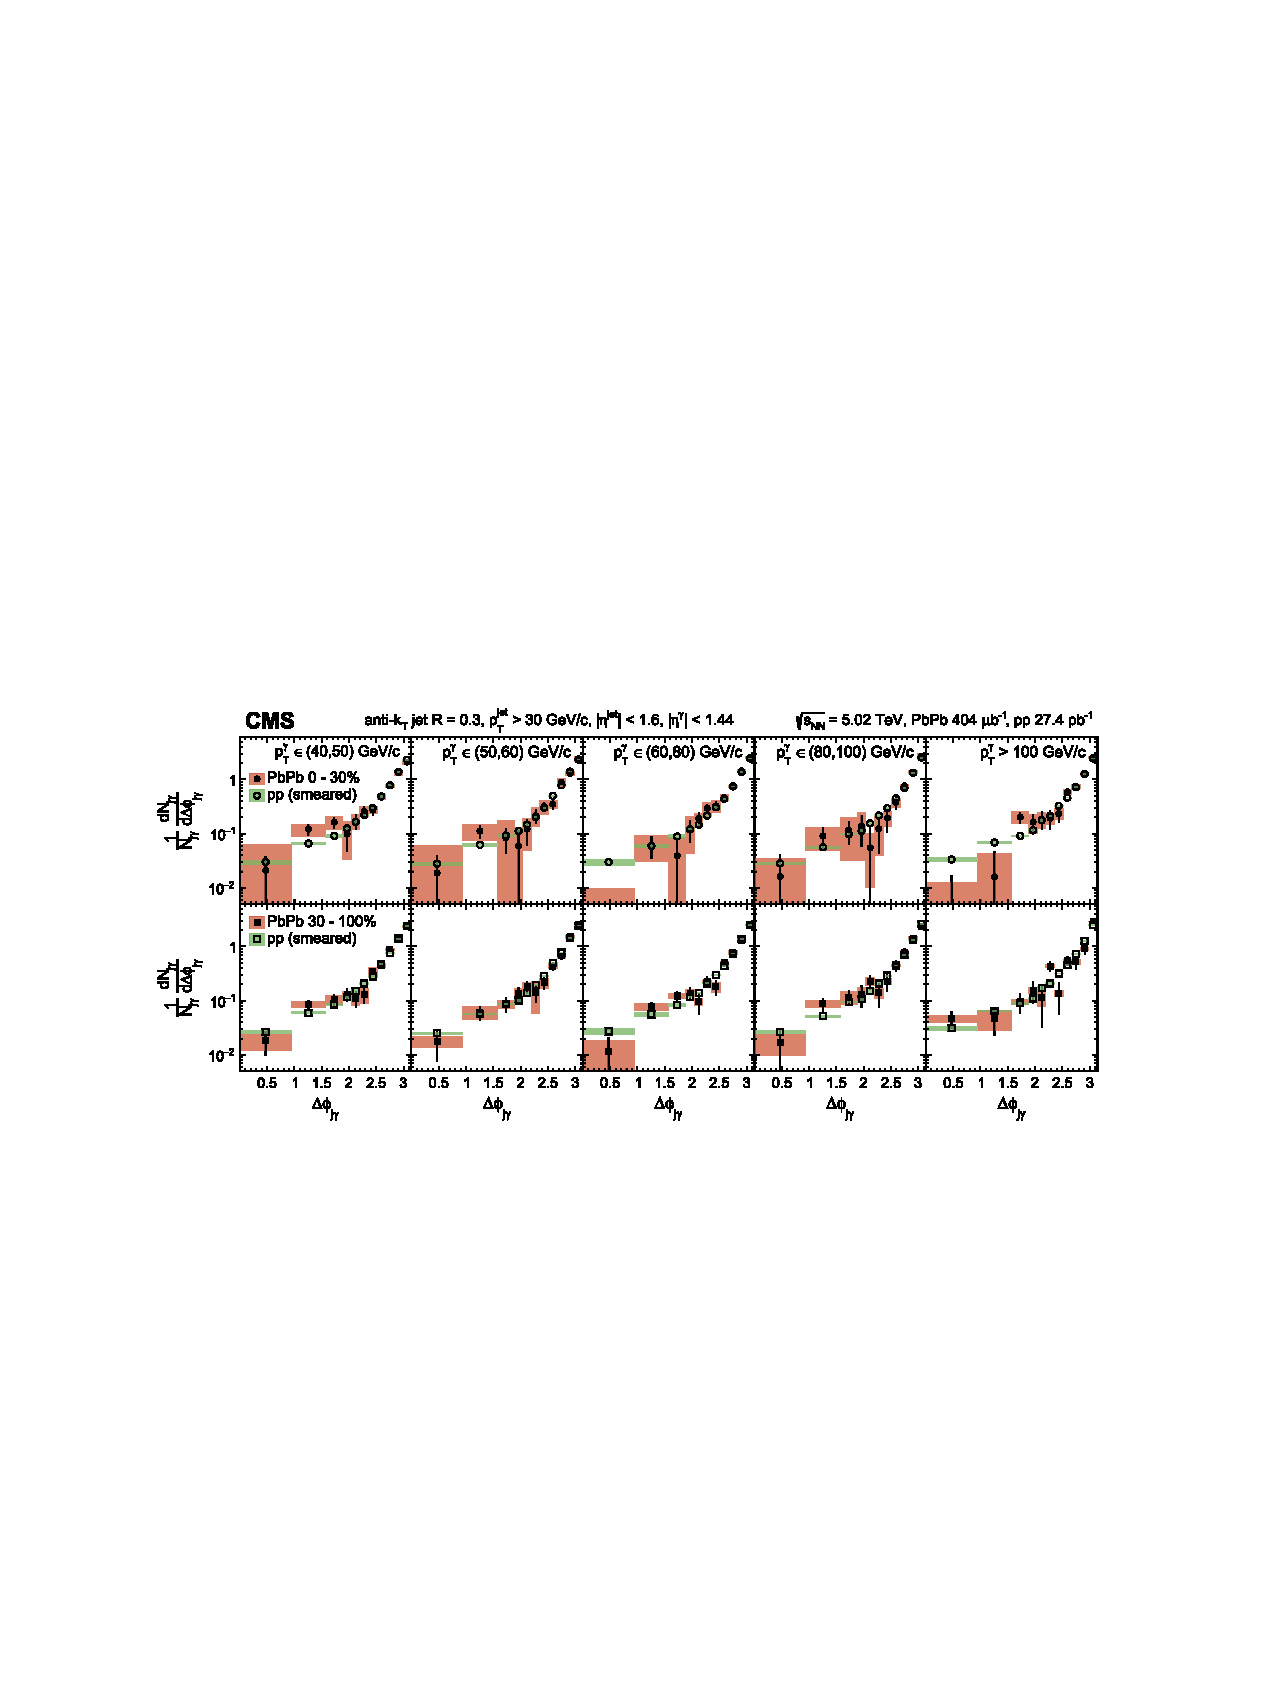
\includegraphics[width=0.99\textwidth]{Introduction/cms_gj_correlations.pdf}
  \caption{The azimuthal correlation of photons and jets in five $\pt^\gamma$ intervals for 0–30\% centrality (top, full circles) and 30–100\% centrality (bottom, full squares) PbPb collisions. The smeared pp data (open symbols) are included for comparison. The vertical lines (bands) through the points represent statistical (systematic) uncertainties \cite{Sirunyan2018}.}
  \label{fig:cms_gj_correlations}
\end{figure}


In conjunction with $\gamma$-jet correlations, the $\gamma$-jet asymmetry, $x_{j,\gamma}\equiv \pt^\mathrm{jet}/\pt^\gamma$ can be measured to quantify in-medium parton energy loss. Derived from Fig.~\ref{fig:cms_gj_correlations}, the jet asymmetry for jets with $\deltaphi > 7\pi/8$ relative to the photon were taken. The asymmetry as a function of photon \pt, as well as the ratio of the number of associated jets per photon in pp and PbPb collisions, $R_{j\gamma}$, is shown in Fig.~\ref{fig:cms_gj_quenching.pdf}~\cite{Sirunyan2018}.

\begin{figure}[htpb]
  \centering
  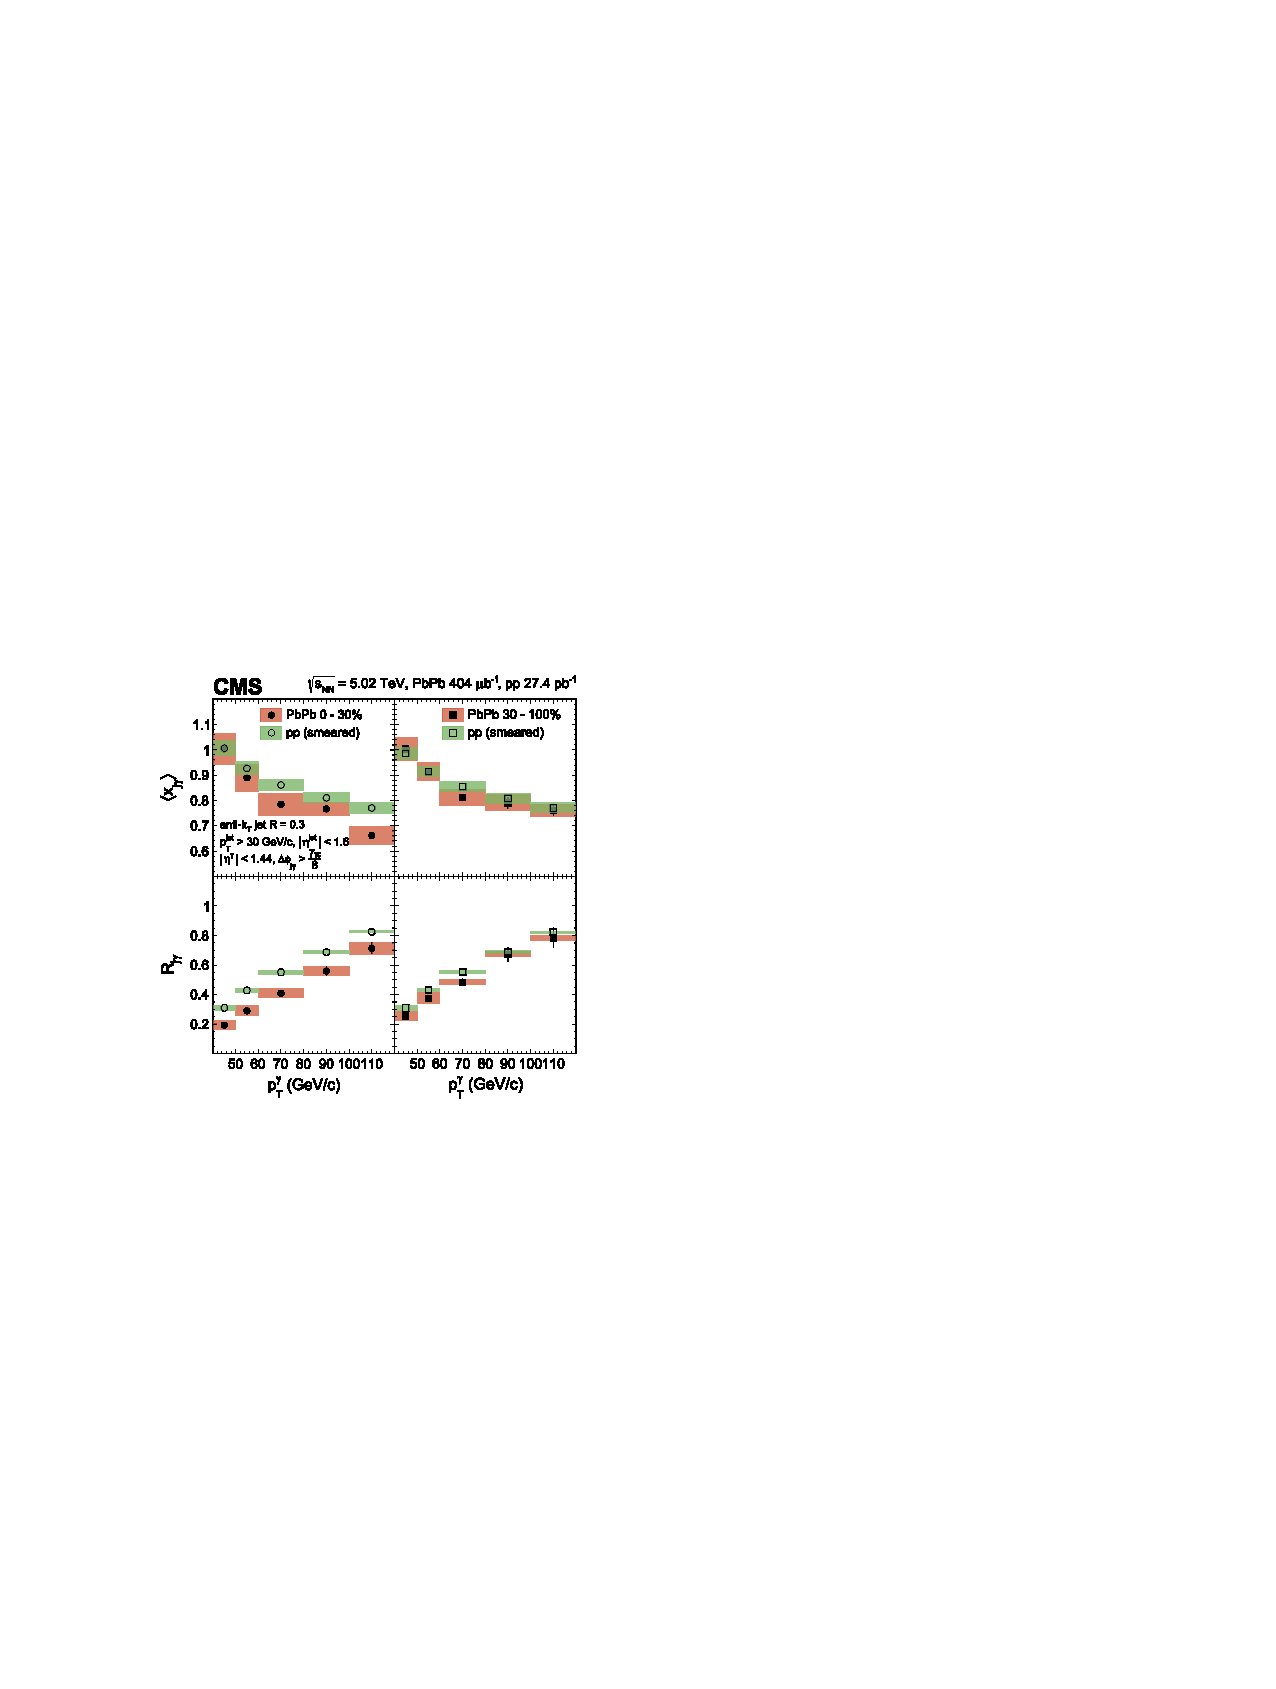
\includegraphics[width=0.8\textwidth]{Introduction/cms_gj_quenching.pdf}
  \caption{The $\langle x_{j,\gamma} \rangle$ values (top) and $R_\mathrm{j\gamma}$, the number of associated jets per photon (bottom), in 0–30\% centrality (left, full circles) and 30–100\% centrality (right, full squares) PbPb collisions. The smeared pp data (open symbols) are added for comparison. The vertical lines (bands) through the points represent statistical (systematic) uncertainties \cite{Sirunyan2018}.}
  \label{fig:cms_gj_quenching.pdf}
\end{figure}

This procedure from CMS also provides a good example of how these correlations are often used to extract other quantities. The angular correlations are measured, from which a region in large $\deltaphi$ is taken (corresponding to the photon and parton being back-to-back). The yields in this region are then reported as a function of fractional momentum, $x_{j,\gamma}$ in order to measure medium effects.

\subsection{$\gamma$-hadron Correlations}
\label{sec:intro_gh}
The leading order picture of prompt photons indicates that the photon and recoiling parton have equal and opposite transverse momenta. Therefore, the measurable quantity, $\zt = p_{\mathrm{T},a}/p_{\mathrm{T},t}$ with the prompt photon as the trigger, is nothing but the fragmentation variable, $p_{\mathrm{T},hadron}/p_{\mathrm{T},parton}$. This explains why prompt $\gamma$-h correlations are such a powerful measurement. They provide a source of recoil partons of fixed momentum and their conditional yields as a function of \zt~in p+p collisions probe the parton fragmentation. By contrast, dihadron and dijet correlations are have the fragmentation function (and therefore any potential medium modifications) folded into the measurement twice, making any observed modifications more difficult to interpret.

When the hadrons roughly opposite the trigger photon are reconstructed as a jet, they are clearly connected to the recoiling parton from the initial scattering in the leading order picture. The hadrons within those jets can then be used to probe the jet fragmentation function. $\gamma$-hadron correlations in which a jet is not reconstructed, however, have a distinct advantage over $\gamma$-jet correlations: hadrons are more sensitive to in-medium modification. Fig.~\ref{fig:raa_particles} shows a minimum in $R_\mathrm{AA}$ for charged hadrons at approximately 6GeV, and a plateau begins after 20 GeV$/c$. It is extremely difficult to measure jets below  $\approx$20 GeV/$c$ in heavy ion collisions due to the large background \cite{STARCollaboration2017}. Selecting jets at higher \pt~(or jets with kinematics similar to that in ``vacuum'', or pp collisions), to avoid this background biases the jet population towards jets that will lose the least energy in vacuum, as discussed in Sec.~\ref{sec:raa}. Additionally, triggering on a high \pt~hadron as a proxy for a jet can bias the measurement towards jets towards the surface of the medium \cite{Zhang2007}. Similar to $R_\mathrm{AA}$, the ratio of the conditional yields for $\gamma$-h and $\gamma$-jet correlations in pp and AA collisions can help quantify medium induced modifications to the parton, in this case, the fragmentation function. Fig.~\ref{fig:phenix_gh_corr} shows the direct\footnote{Direct is used in lieu of prompt at RHIC due to the smaller contribution of fragmentation photons at the lower center of mass energies compared to LHC. Direct here means non-fragmentation prompt photons, or photons produced directly in 2-to-2 scatterings.} photon-hadron correlations measured with the PHENIX detector as a function of $\xi\equiv\ln(1/\zt)$:

\begin{figure}[htpb]
  \centering
  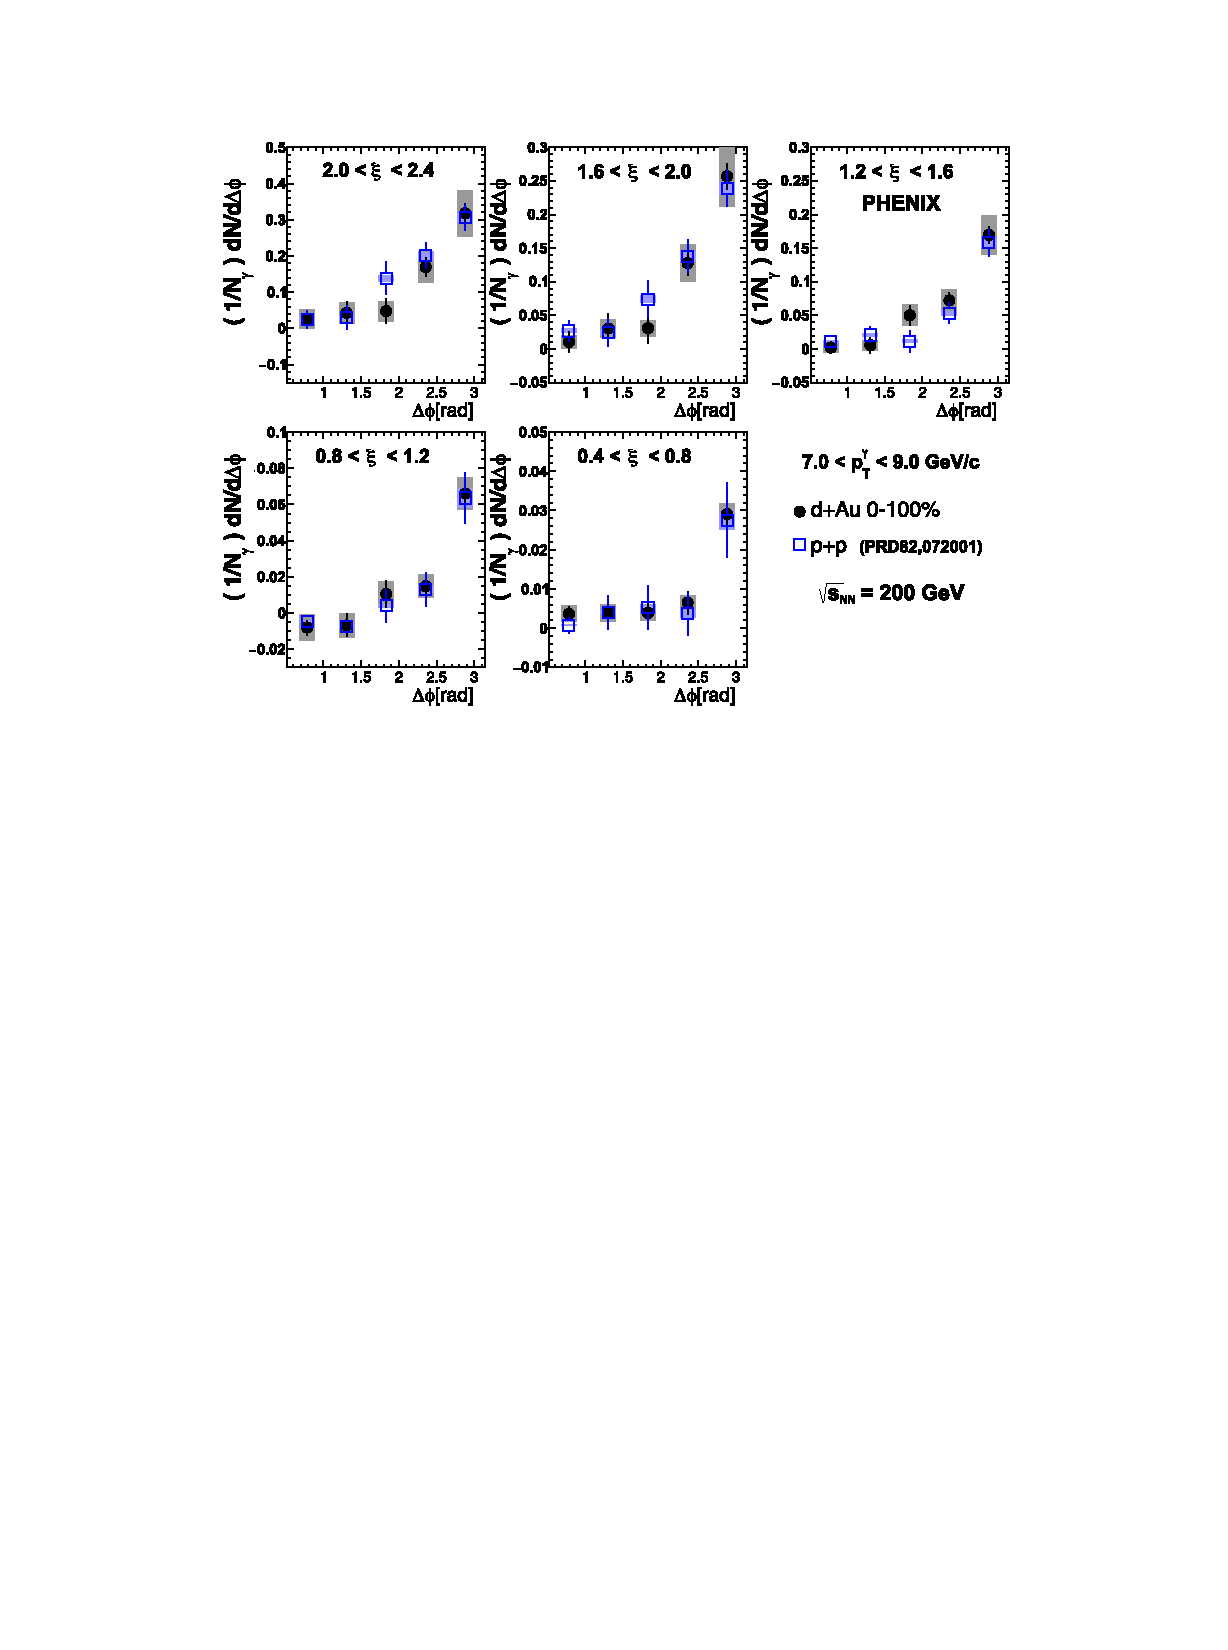
\includegraphics[width=0.8\textwidth]{Introduction/phenix_gh_corr.pdf}
  \caption{Per-trigger yield of hadrons associated with direct photons in Au+Au collisions (closed [black] circles) for direct photon \pT~5–9 GeV/$c$, compared with p+p baseline (open [blue] squares), in various $\xi$ bins \cite{PHENIXCollaboration2020}.}
  \label{fig:phenix_gh_corr}
\end{figure}

Similar to the $\gamma$-jet measurement in the previous section, the conditional yield at higher \deltaphi~is measured. This conditional yield as a function of $\xi$ is the experimentally measured fragmentation function. The ratio of this yield in pp and AA collisions, $I_\mathrm{AA} \equiv Y_\mathrm{AA}/Y\mathrm{pp}$, is a nuclear modification factor which quantifies the difference between the fragmentation functions in AA and p+p collisions. This is shown in Fig.~\ref{fig:phenix_gh_IAA} \cite{PHENIXCollaboration2020}. 

\begin{figure}[htpb]
  \centering
  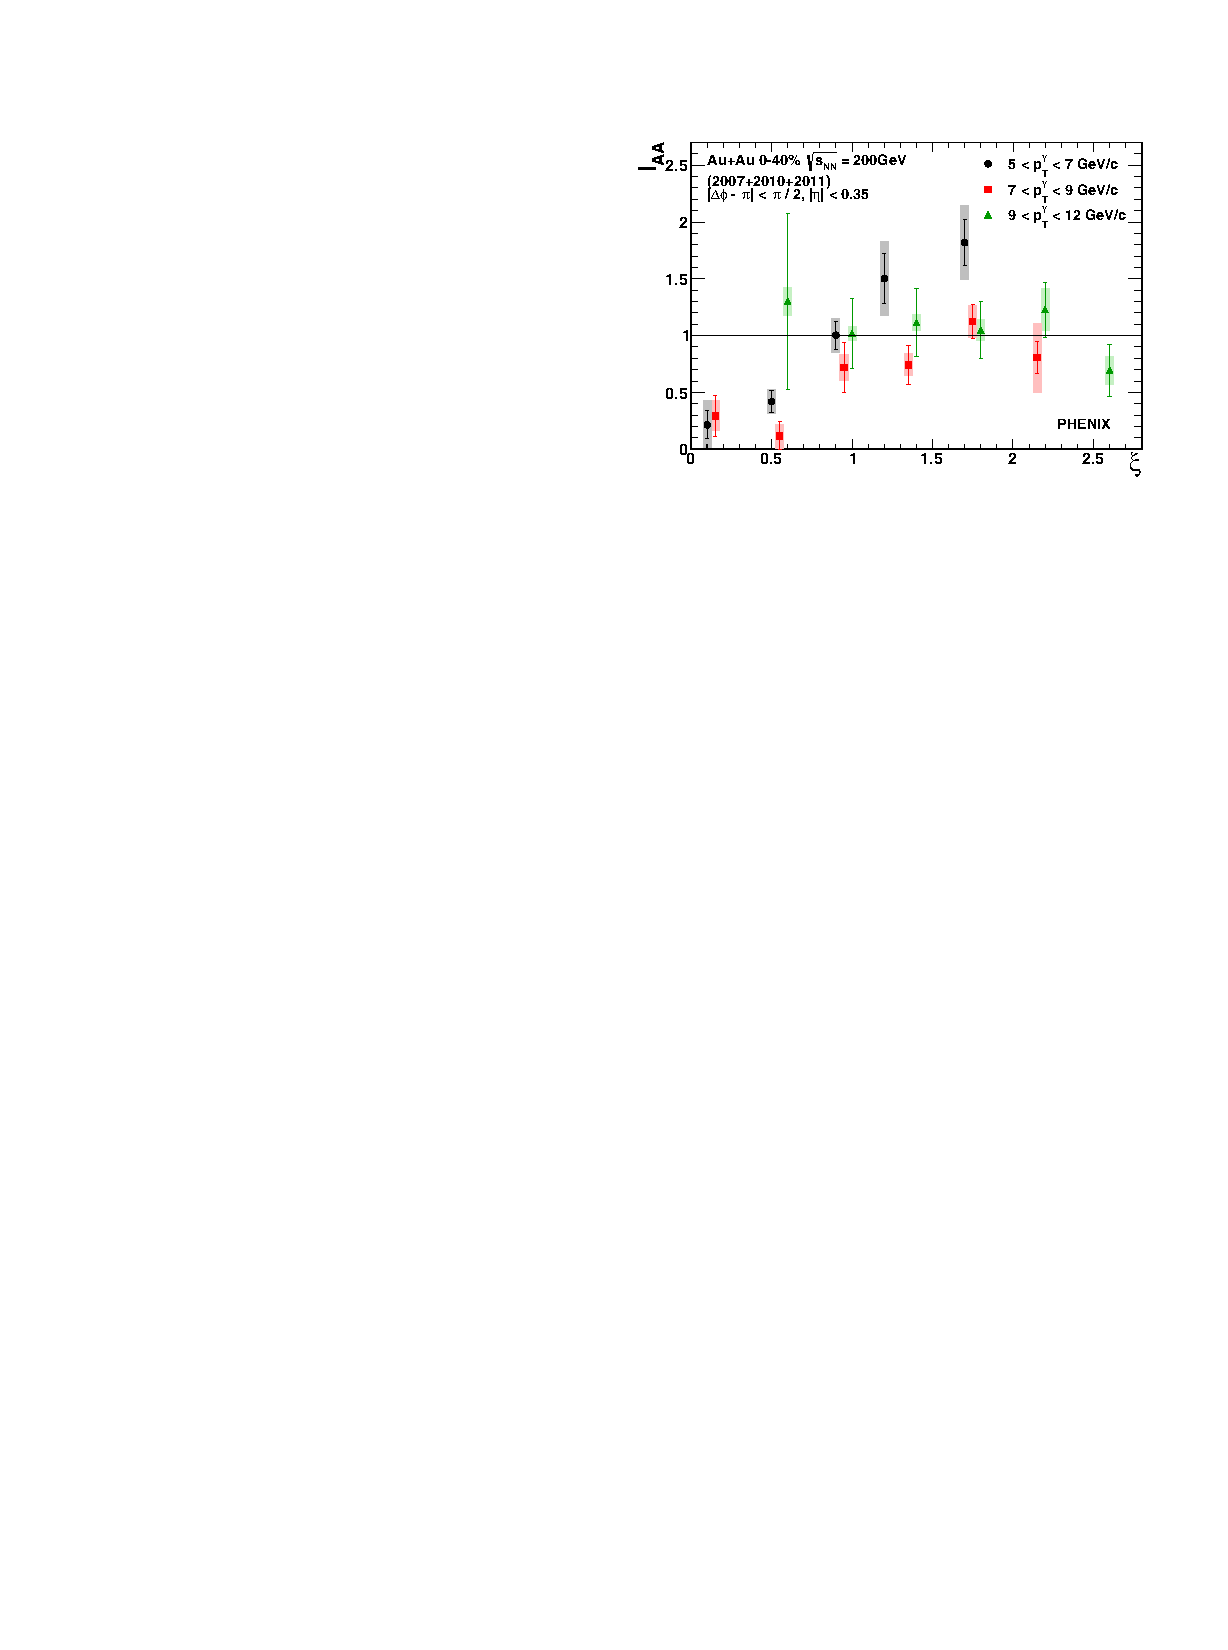
\includegraphics[width=0.8\textwidth]{Introduction/phenix_gh_IAA.pdf}
  \caption{$I_\mathrm{AA}$ for three direct photon $\pt^\gamma$ bins \cite{PHENIXCollaboration2020}.}
  \label{fig:phenix_gh_IAA}
\end{figure}


$\gamma$-hadron correlations are an incredibly powerful tool: they provide an observable that probes the parton fragmentation function with objects in the collision (low to intermediate \pt hadrons) that are particularly sensitive to medium modifications. Measuring $\gamma$-hadron correlations in both pp and PbPb collisions is an important step in elucidating the modifications to the parton fragmentation function due to QGP. However, a full understanding of these phenomena requires measurements of cold nuclear matter (CNM) effects, which should be present in A+A collisions but are difficult to distinguish experimentally from effects due to interactions with the medium.

% advantage of gamma-hadron over gamma-jet: hadrons in intermediate pT range are more sensitive to modification, as seen in raa plot for hadrons. Jets may potentially suffer from suvivorship bias, in wich jets selected based on kinematics matching vaccuum jets will lose the least energy.  

% For γ − h correlations, on the other hand, the conditional yield should be much more closely related to the fragmentation function. In the leading order picture, the direct photon exactly balances the away-side jet and therefore, the measurable quantity, pT,a/pT,t, is nothing but the fragmentation variable pT,a/pT,jet. This explains why γ − h correlations are a powerful measurement. They provide a source of recoil partons of fixed momentum. Their conditional yields in p + p collisions only probe the jet fragmentation. By contrast, hadron correlations are controlled by the jet cross section which also depend on the PDF’s and the parton scattering cross sections.
\section{Cold nuclear Matter Effects}
In order to quantitatively study the properties of the QGP, it is necessary to separate effects which are due to interactions with the medium from those which are intrinsic to the structure and interactions of cold nuclei. The p + p baseline measurements used to calculate the nuclear modification factor $R_\mathrm{AA}$ can not account for these nuclear effects, since none are present in free protons. For example, $^{208}$Pb contains 126 neutrons, so the majority of neucleon-neucleon collisions in PbPb events will involve neutrons. Any isospin dependent effects would be impossible to model in pp collisions due to the absence of initial neutrons in the system.

\subsection{The Nuclear Parton Distribution Function}
The production cross sections for prompt photons and hadrons should be sensitive to the distribution of quarks and gluons inside the nucleus, detailed by the nuclear parton distribution function (nPDF). More specifically, the nPDF is defined as the probability density for finding a parton with a certain longitudinal momentum fraction $x$ at resolution scale $Q^2$ within a nucleon bound within a nucleus. The relation of the bound-proton PDFs with respect to free proton PDFs $f_i^p$ is often expressed in terms of a nuclear modification factor in the form of:

\begin{equation}
  R_i^A(x,Q^2) = \frac{f_i^p/A(x,Q^2)}{f_i^p(x,Q^2)} 
\end{equation}

A typical form of such modifications is shown in Fig.~\ref{fig:cnm_cartoon}.

\begin{figure}[htpb]
  \centering
  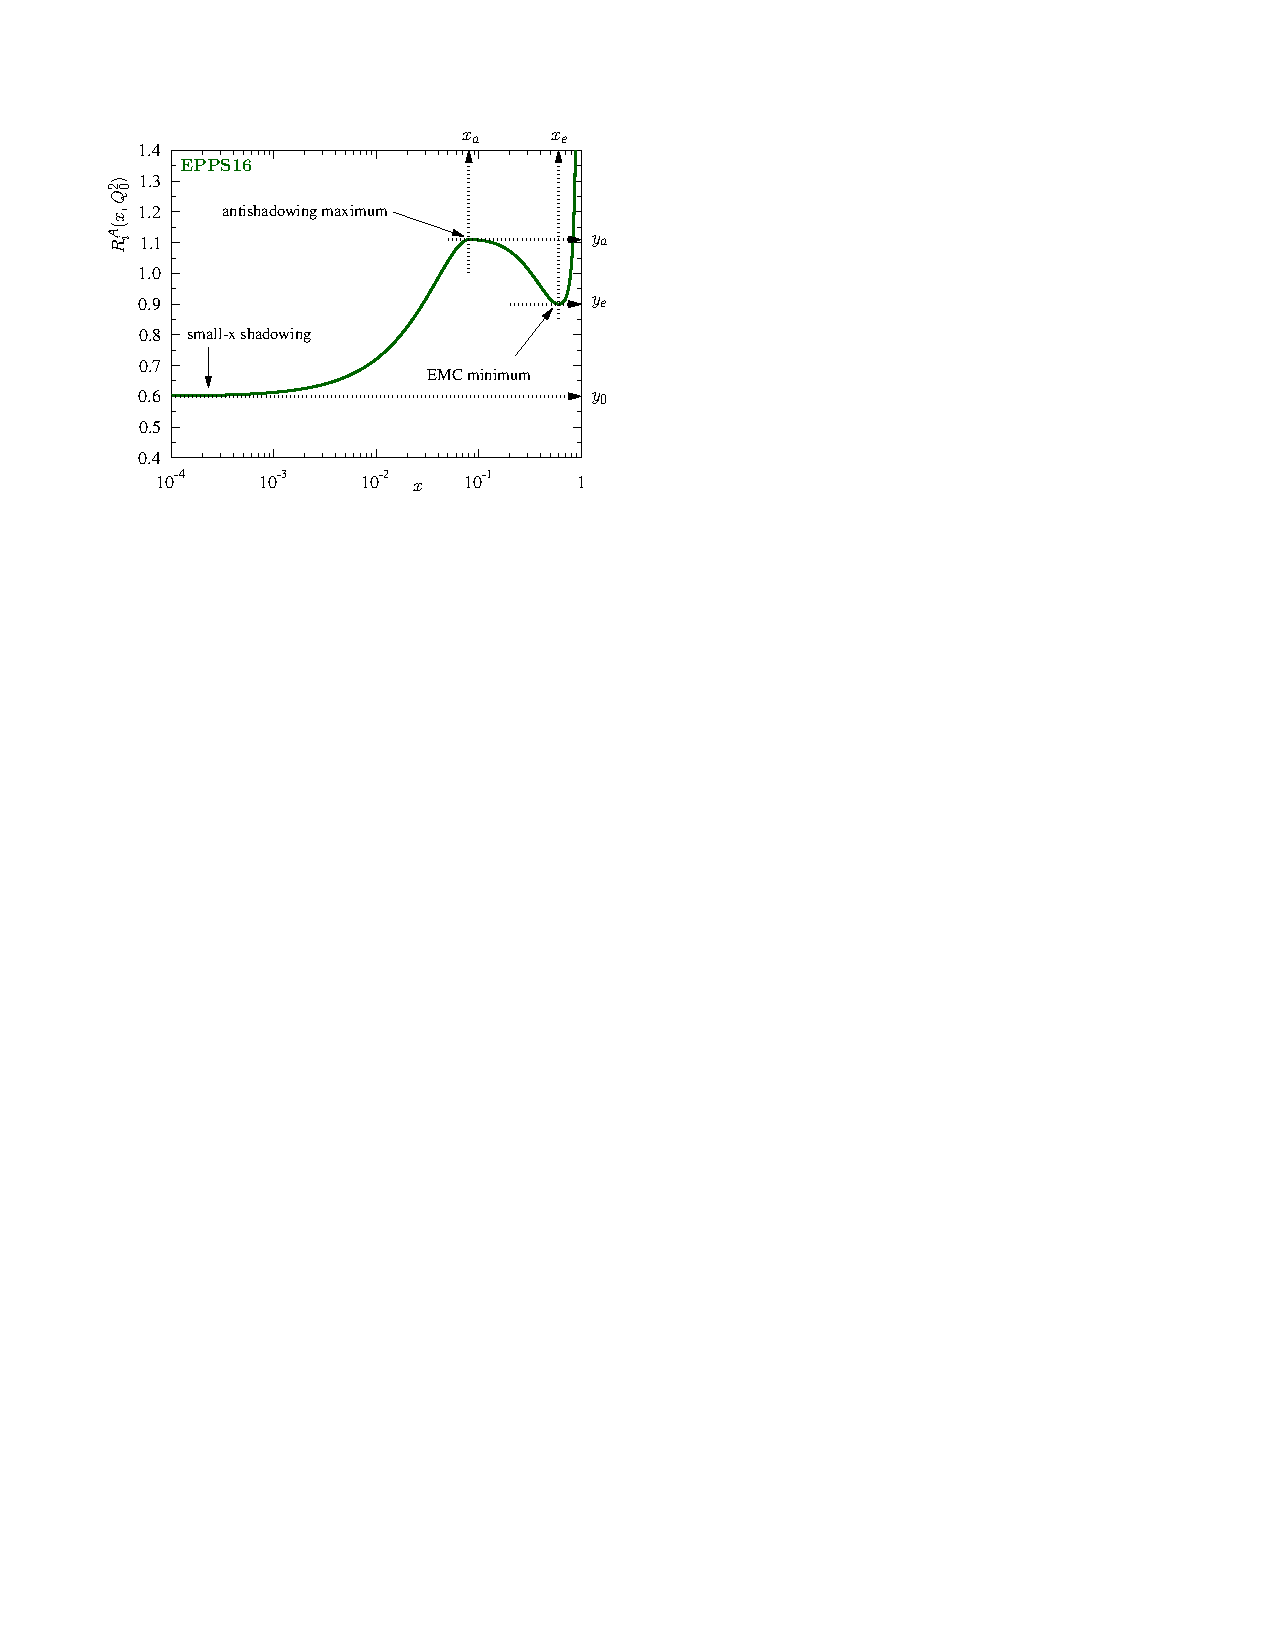
\includegraphics[width=0.8\textwidth]{Introduction/cnm_cartoon}
  \caption{Typical form of PDF modifications in a nucleus\cite{Pumplin2001}.}
  \label{fig:cnm_cartoon}
\end{figure}

The modification in the region where the ratio is less than 1.0 is called ``shadowing'' at very low $x$.  The ``EMC'' effect occurs at  $0.3 < x < 0.7$. The region where the modification is larger than 1.0 is called ``anti-shadowing''~\cite{Pumplin2001}. The shadowing and antishadowing effects reflect interaction of the scattered parton and the nuclear background color field that lead to a suppression or enhancement of inclusive hadron production in theoretical calculations \cite{epps16:2017}. The origin of the EMC effect is still not thoroughly understood, but is often attributed to either mean-field modifications or short-ranged correlated pairs \cite{Hen2017a,Norton2003a}. The exact magnitude of these effects on various measurements, as well as an improved understanding of the nPDF's is a currently under investigation in the field. Recently, a major step forward toward this goal has been the inclusion of LHC pPb data, particularly for extracting the gluon PDF.
\subsection{Nuclei and Fragmentation}

Aside from differences between the PDFs in free and bound nucleons, there are potential observable effects of the nucleus as a medium itself. Measurements in p+A collisions showed that particle production at moderate transverse momentum increases faster than the number of binary nucleon-nucleon collisions. This was attributed to the Cronin effect where the scattered parton undergoes multiple scatterings in the nucleus, resulting in a transverse momentum boost, \textit{before} the interaction that ultimately produces the final state particle \cite{Cronin1975}.

Currently, however, an open question in the field is the exact timescale of fragmentation, as both pQCD and lattice calculations are unable to provide estimates. This leaves open the possibility that the parton begins to fragment while still inside the nucleus, potentially modifying the fragmentation process and the final state hadrons of the resulting jet.


The current state of understanding on cold nuclear matter effects modifying the parton fragmentation function is ambiguous: In di-hadron and direct photon-hadron correlations, no significant modification of the jet fragmentation was observed in measurements by the PHENIX collaboration in d--Au collisions at a center-of-mass energy of 200 GeV~\cite{Adler:2005ad} and the ALICE collaboration in \pPb~collisions at 5.02 TeV~\cite{Acharya:2018edi,Adam:2015xea} at mid rapidity. At forward rapidity, probing a lower-x regime, a strong-modification was observed by the PHENIX collaboration in d-Au collisions~\cite{Adare:2011sc}. A more recent measurement by the PHENIX collaboration with pp, p--Al, and p--Au data revealed a transverse momentum broadening consistent with a path-length dependent effect~\cite{Aidala:2018eqn}. However, a recent ATLAS measurement of the jet fragmentation function in \pPb~collisions showed no evidence for modification of jet fragmentation for jets with $45<\pt<206$ \GeVc~\cite{Aaboud:2017tke}. Measurements of the fragmentation of jets with much lower momentum are necessary to limit the Lorentz boost to the timescales of fragmentation, as such a boost may result in fragmentation outside the nucleus. These measurements would test the $Q^{2}$ evolution of fragmentation functions in cold nuclear matter, testing factorization theorems that are neither proven nor expected to hold in general for collisions involving nuclei~\cite{deFlorian:2011fp}. 

\section{Statement of Purpose}

Parton fragmentation may be modified in the nucleus, offering a way to explore the dynamics of QCD in nuclei including elastic, inelastic, and coherent multiple scattering of partons. Moreover, the known spatial dimensions of nuclei provide a filter possibly shedding light on the timescale of the fragmentation process, which remains unknown~\cite{Accardi:2009qv,Accardi:2012qut}. Additionally, because photons produced in hard scatterings do not strongly interact, they constrain the parton kinematics from the same scattering before any modification. Thus, measurements of photon-tagged jet fragmentation in pA collisions serve as a powerful tool to study multiple-scattering effects in cold nuclear matter~\cite{Xing:2012ii}, which serve as a control for effects of the quark$-$gluon plasma (QGP) in nucleus$-$nucleus collisions, where modifications of the jet spectrum, fragmentation, and substructure have been observed~\cite{Connors:2017ptx}.

Experimental data \cite{Chatrchyan2014} on dijet spectra in p + Pb collisions at $\sqrtsNN$= 5.02 TeV, show no significant effect of jet quenching within the experimental errors in the nuclear modification of the dijet asymmetry in transverse momentum. Additionally, since trigger biases in dihadron and dijet measurements prefer surface and tangential configurations for coincident production of hadrons or jets \cite{Zhang2009}, the effect of jet quenching is expected be smaller than in $\gamma$-hadron production where the direct photon does not have strong interaction with the hot medium before being detected. 

In this work, azimuthal correlations of charged hadrons with isolated photons, $\gammaiso$, are analyzed in \pPb~and pp collisions with a center-of-mass energy of \sqrtsNN~ = 5.02 TeV. Isolated photons are measured at midrapidity, {$|\eta|<0.67$}, and with transverse momenta in the range $12 <\pt<40$ \GeVc, which yields the scaling variable {$x_{\mathrm{T}} = 2\pt/\sqrt{s_{\mathrm{NN}}}\ = $ 0.005--0.016}. The kinematic range probed in this analysis offers access to a lower $Q^{2}$ than other LHC experiments, which is where the largest nuclear effects can be expected,  and we cover a similar $x_{\mathrm{T}}$ range as RHIC measurements at forward rapidity~\cite{Adare:2011sc}, where cold nuclear matter effects were observed in dihadron collisions. 

Understanding the dynamics of quarks and gluons in nucleons and nuclei is a key goal of modern nuclear physics. Proton$-$nucleus (pA) collisions at high energies provide information about the parton structure of nuclei, parton$-$nucleus interactions, and parton fragmentation in a nuclear medium~\cite{Accardi:2009qv}. The energy of the Large Hadron Collider (LHC) available for pA collisions is a factor of 25 larger than at the Relativistic Heavy Ion Collider (RHIC), and thus it provides unprecedented reach in longitudinal momentum fraction Bjorken-$x$ and $Q^{2}$~\cite{Salgado:2011wc}. 

% The measurement of the transverse momentum of $\gammaiso$ constrains the recoiling parton kinematics in a way that is not possible with inclusive jet production and provides an effective way to probe the nuclear modification of the fragmentation function. Moreover, the per-trigger yield is the ratio of a semi-inclusive cross-section (photon + jet) and inclusive cross-section (photon). Both quantities are sensitive to the nuclear parton distribution functions (PDF) in the same way \cite{kang2016semiinclusive,gamma_cross_section}. Thus, by measuring per-photon quantities, sensitivity to the nuclear PDF is eliminated.
%end

\chapter{Experimental Apparatus} 
A Large Ion Collider Experiment (ALICE) is the only experiment at the Large Hadron Collider (LHC) dedicated to studying heavy-ion physics. Its detectors measure and identify hadrons, electrons, photons, and muons. The ALICE detectors are optimized for the study of heavy-ion collisions up to the highest energy available. and is designed to be simultaneously capable of measuring  bulk properties of the collision involving soft hadronic interactions and large cross section physics, and capable measuring rare probes involving small cross section physics. In particular, ALICE was designed to track and identify particles from very low,  \~100 MeV, up to fairly high, \~100 GeV, transverse momenta in an environment of extreme particle density. This chapter will first briefly discuss the LHC particle accelerator, followed by a description of the subdetectors and triggering system of ALICE.

\section{The Large Hadron Collider} 
\label{sec:LHC}
The LHC is the largest particle accelerator ever made. Located near at CERN near Geneva, Switzerland  it was optimized to collide protons up to a center-of-mass energy of \sqrts=14 TeV, and heavy ions (including Pb, Ar, and Xe) up to \sqrtsNN=5.5 TeV \cite{Evans2008}.

The LHC was designed to supply a luminosity of $\mathcal{L}=10^{34}$cm$^-2$s$^-1$ for proton-proton collisions, and a luminosity of $\mathcal{L}=10^{34}$cm$^-2$s$^-1$. The proton-proton luminosity was driven by the search for the Higgs boson, with CMS and ATLAS considered as the high luminosity experiments at the LHC. ALICE, on the other hand, is the only dedicated heavy-ion experiment at CERN. The LHC was constructed using the existing tunnel of the Large Electron-Positron Collider (LEP), operational until 2000. The LHC consists of 4 major components:

\begin{enumerate}
	\item Dipole magnets that bend the beam on its orbit with a maximum magnetic field of 8.33 T. 
	\item Quadrupole, sextupole, octupole and decapole magnets the focus the beams.
	\item Acceleration cavities that increase the beam energy.
	\item Two beam pipes with an ultra-high vacuum  which contain the two beams.
\end{enumerate}

The magnetic field in the dipoles is provided by superconducting magnets which are filled with liquid helium. The helium is cooled down to 1.9 K in order to reach the super-fluid state. To reduce the number of interactions of the beam with the environment or air, an ultra-high vacuum is kept in the beam pipes reaching a quality of $10^{-13}$ atm over a total volume of 150~m$^3$ \cite{Evans2008}.

The LHC has eight possible interactions points, four of them are equipped with large detector systems shown in Figure 3.1. ALICE is the only dedicated heavy-ion experiment, and will be described in the next section. The detectors systems of ATLAS (A Toroidal LHC Apparatus) and CMS (Compact Muon Solenoid experiment) were designed as general purpose detectors primarily in pursuit of the Higgs-boson and its properties, as well as precision measurements of the Standard Model particles and searches for physics beyond the Standard Model. Although both detectors have not been optimized for heavy-ion collisions, they contribute extensively to the high \pt~analysis in Pb–Pb collisions profiting from their large pseudorapidity coverage, their excellent high luminosity capabilities, and their high momentum resolution. The LHCb (LHC beauty) experiment dedicated its research program to the search for CP-violation in the B-meson system, as well as precision measurements in the charm and beauty quark sector.

\begin{figure}[htpb]
  \centering
	\includegraphics[width=0.79\textwidth]{Experimental_Aparatus/LHC.png}
	\label{fig:lhc}
	\caption{Overview of the CERN accelerator complex and the injection chains used for the LHC with their respective top energies for protons and ions after the respective accelerator \cite{Mobs:2197559}.}
\end{figure}

\FloatBarrier

\section{A Large Ion Collider Experiment}
\label{sec:ALICE}
ALICE – A Large Ion Collider Experiment – is the only LHC experiment dedicated to study of heavy-ion physics. Therefore, its aim is not to find signatures rare particles in pp collisions as is the primary focus of the other three major LHC experiments, but instead to collect as much data as possible from the large heavy-ion event. This imposes strong demands on the detector. A Pb–Pb collision typically produces approximately 500-1000 charged particles per pseudo-rapidity unit ($\text{d}N_{ch}/\text{d}\eta \approx 2000$), and can reach as high as $\text{d}N_{ch}/\text{d}\eta \approx 2000$ in the most central collisions \cite{ALICECollaboration2016}. Fig.~\ref{fig:alice} shows an overview of the ALICE detector.


\begin{figure}[htpb]
  \centering
  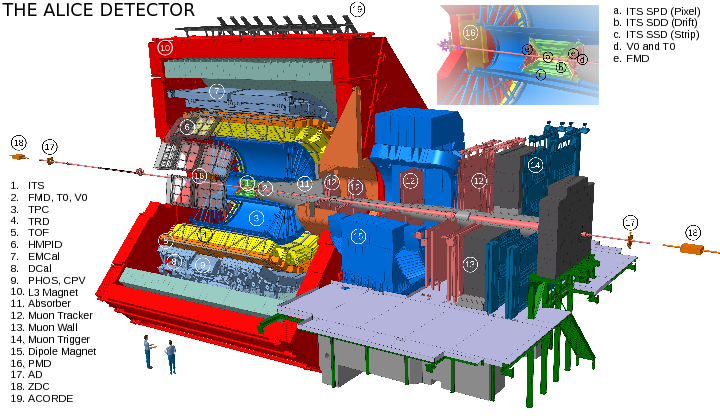
\includegraphics[width=0.99\textwidth]{Experimental_Aparatus/ALICE.png}
  \caption{Schematics of the ALICE detector \cite{Tauro:2263642}.}
  \label{fig:alice}
\end{figure}

As shown in Fig.~\ref{fig:alice}, ALICE can be conceptualized as consisting of three major parts:

\begin{enumerate}
    \item The central barrel contained inside the magnet with an acceptance in pseudo-rapidity of $-0.9 \leq \eta \leq 0.9$ over the full azimuth angle;
    \item The muon spectrometer at pseudo-rapidity of $-4.0 \leq \eta \leq -2.4$; 
    \item Various multiplicity detectors at $-3.4 \leq \eta \leq 5.1$
\end{enumerate}

The central barrel resides within the L3 magnet, a warm solenoid magnet with a magnetic field of B = 0.5 T. The muon spectrometer extends only in the forward region (C side) and contains a dipole magnet (B = 0.67 T) which bends the muons away from the interaction vertex in the horizontal plane.Lastly, the multiplicity detectors are arrays of scintillator counters, with one in each of the forward regions.

\subsection{Inner Tracking System}
\label{sec:ITS}
Closest to the interaction point, in the middle of the central barrel, is the Inner Tracking System (ITS) that covers the pseudorapidity window $|\eta| < 0.9$. The ITS is used for triggering and high-resolution tracking and consists of six concentric layers of silicon detectors surrounding the beam pipe: two layers each of Silicon Pixel Detectors (SPD), Silicon Drift Detectors (SDD), and Silicon Strip Detectors (SSD). 

A schematic overview is given in Fig.~\ref{fig:ITS}. The main purposes of the ITS are to accurately measure the position of the collision vertex and secondary vertices from weakly decaying particles (in particular strange hadrons and B and D mesons, which have typical decay lengths of a couple of cm), measure the \pt and position of charged particle tracks -- often complementing TPC tracking information -- and, in the case of the SPD, to provide triggering input for the entire detector. This detector system has a very fine granularity, resulting in a high tracking and vertexing resolution even in extremely high multiplicity environments. The resolution for each subsystem is summarised in Table~\ref{tab:its}. Moreover, due to its proximity to the beam pipe, a high momentum resolution and large specific energy loss range, particle identification is possible below the lower momentum limit of the TPC (approximately\~ 150 MeV).

\begin{figure}[htpb]
  \centering
  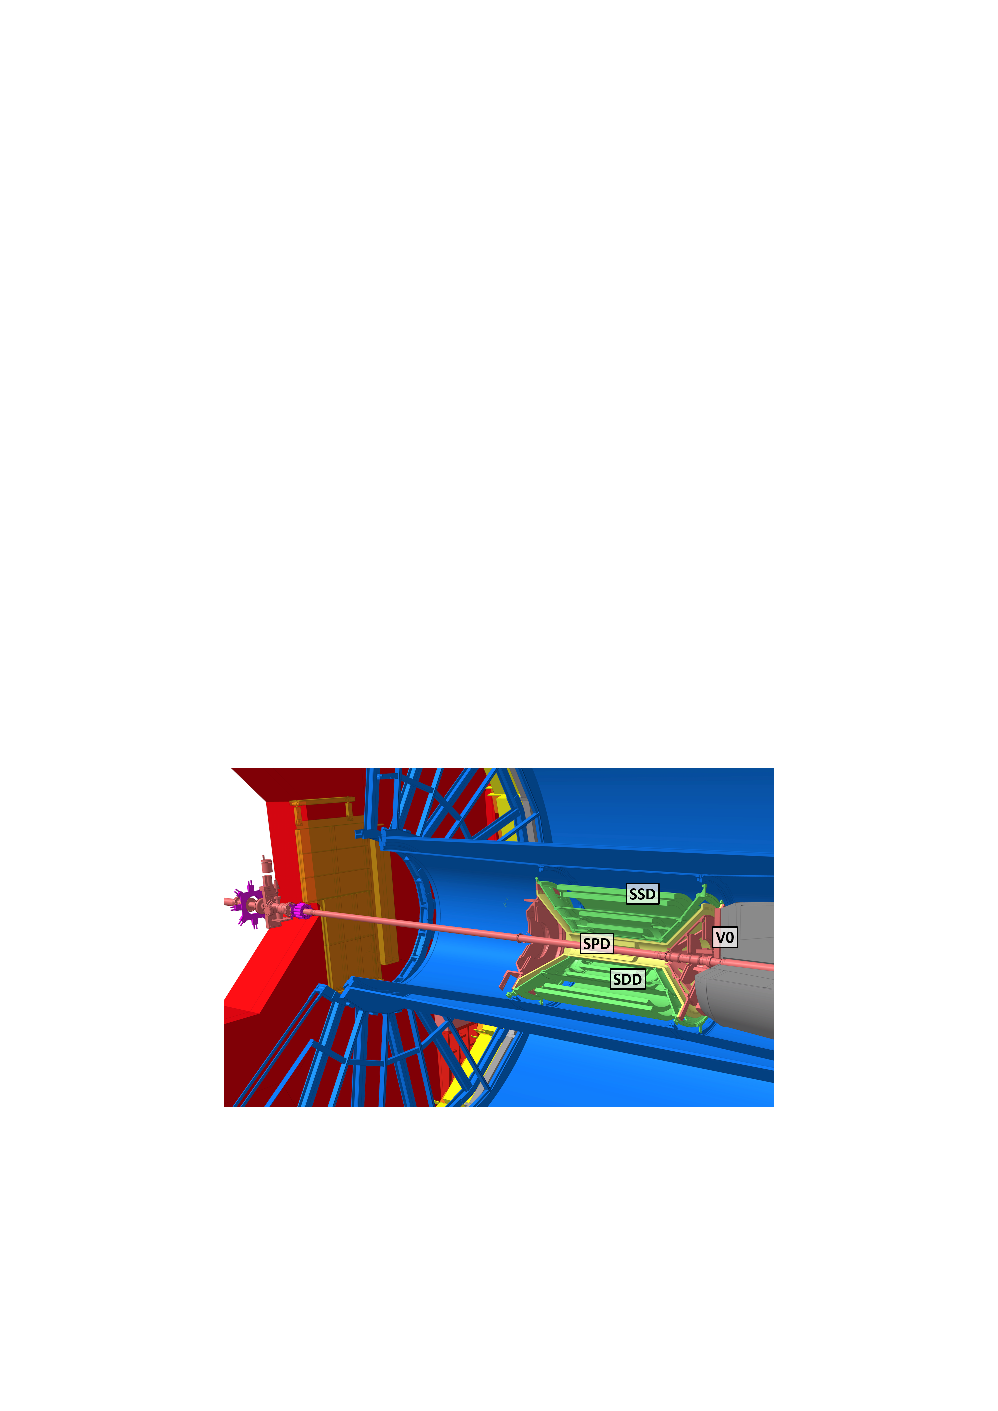
\includegraphics[width=0.8\textwidth]{Experimental_Aparatus/ITS.pdf}
  \caption{Schematics of the Inner Tracking System and nearby detector components, modified from \cite{Tauro:2263642}. The V0 detector is only shown on the C side.}
  \label{fig:ITS}
\end{figure}

\begin{table}
\centering
\begin{tabular*}{0.6\columnwidth}{@{\extracolsep{\fill}}ccc@{}}
        \hline
	Detector & $r\varphi$ precision ($\mu$m) & $z$ precision ($\mu$m)\\
	\hline
	SPD & 12 & 100 \\
	SDD & 35 & 25 \\
	SSD & 20 & 830 \\
	\hline
\end{tabular*}
\end{table}


The ITS is a silicon based detector. Silicon is a semiconductor meaning it has a valence band and a conduction band separated by a band gap. The basic operating principle is as follows: a pn junction is used where a reverse bias is applied that depletes the active area of charge carriers. When a charged particle hits the detector, it will create electron-hole pairs along its trajectory that will in turn generate a current pulse, as shown in Fig.~\ref{fig:silicon}. The current will then traverse the electric field and eventually be collected at electrodes connected to a current amplifier. For the purposes of charged particle tracking with the ITS, the only relevant information is whether a particle has hit the detector. This is ensured by triggering if the pulse is above a certain threshold. The advantages of using a semiconductor are that this creates a fast signal, one can achieve a very high tracking resolution, and it has a low material thickness, since the electron diffusion length is only a few $\mu$m.

\begin{figure}[htpb]
  \centering
  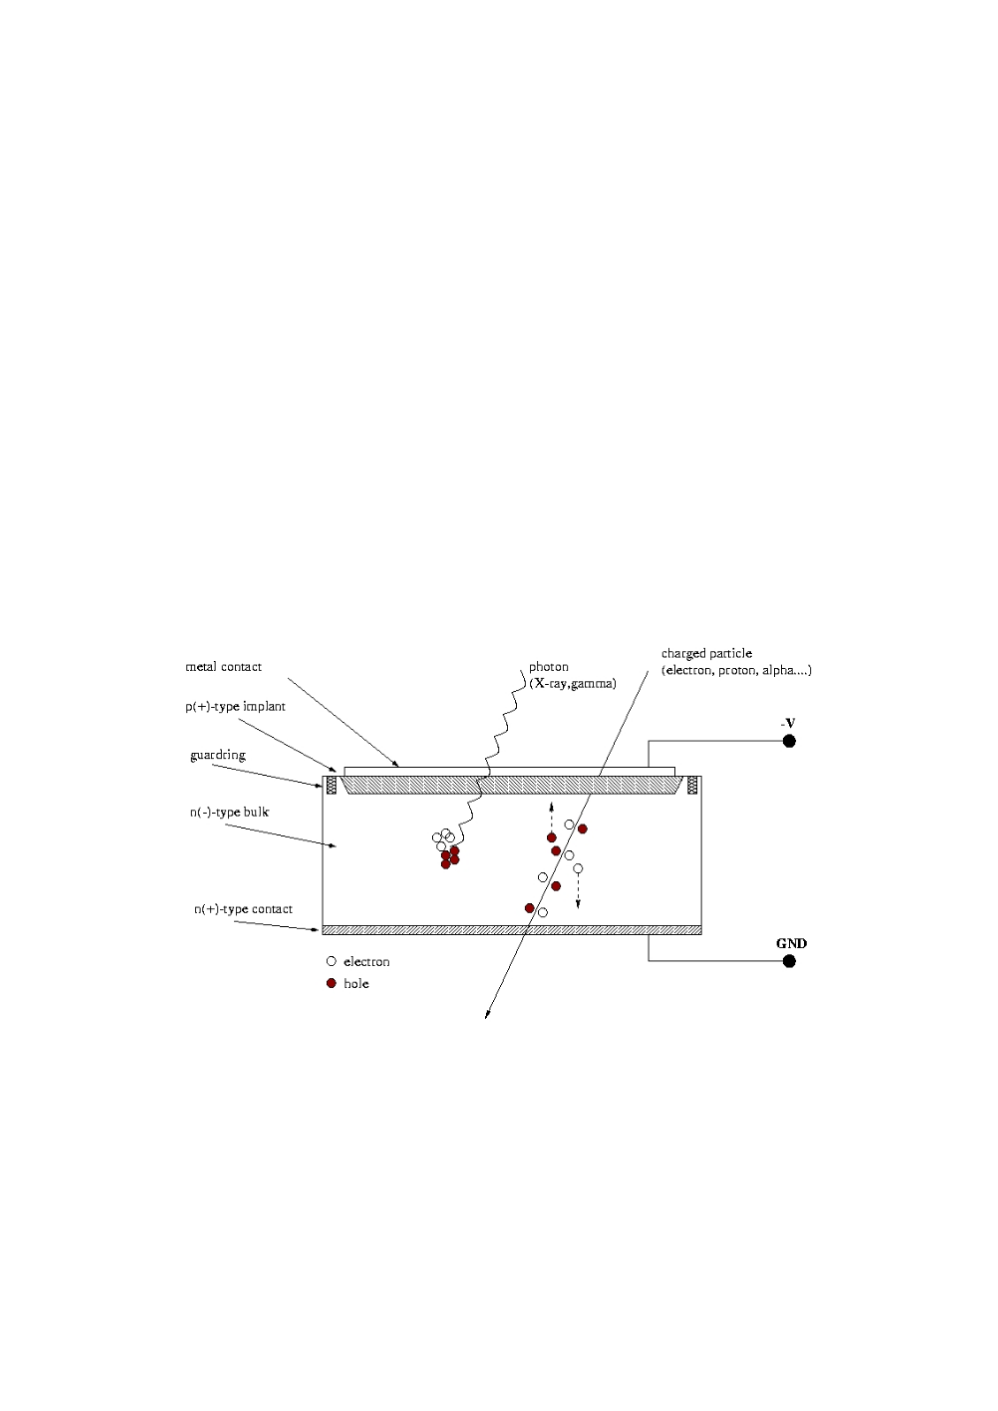
\includegraphics[width=0.8\textwidth]{Experimental_Aparatus/silicon_detector.pdf}
  \caption{Basic principle of a semiconductor detector. When a charged particle traverses the detector, it excites electrons from the valence band to the conduction band, which creates electron-hole pairs. The applied electric field will cause these to drift towards the metal contacts, which generates a current pulse that can be detected. \ref{Adolfsson:2750097},}
  \label{fig:silicon}
\end{figure}

Each subdetector of the ITS uses a different technology. The SPD is built of pixels of silicon diodes, each measuring 50×425 $\mu$m$^2$. These are read out by 1200 chips per layer, each covering 8192 cells, totalling 9.8$\times$106 cells per layer. The two SPD layers are located 3.9 and 7.6 cm from the beam axis, respectively, and extend 282 mm in the longitudinal direction.

The SDDs are built of 260 drift cells distributed over the two layers, where the drift time of charge carriers is measured in order to precisely determine where the track has interacted with the cell. Each cell has 256 collection anodes mounted to it along the z axis with a spacing of 294 $\mu$m. The drift regions are 35mm long and extend in the $\varphi$ direction. To determine the $r\varphi$ coordinate, the drift velocity is monitored by MOS injectors in the substrate that are triggered during gaps in the LHC bunch crossing schedule so they do not interfere with collisions. The position is determined by integrating the velocity over the time measured at the anode. The effective cell length is $\leq 202\mu$m. These detectors are able to measure the number of collected charge carriers, which is proportional to the energy deposited per unit length, dE/dx, and therefore can be used for PID. The two SDD layers are located 15.0 and 23.9 cm from the beam axis and have lengths of 443 and 593 mm in the z direction.

Finally, the SSDs each consist of a double layer of silicon strips placed at an angle of 35 mrad ($\approx 2\textdegree$) relative to each other. When a particle crossing one of the SSDs yields a signal in both strip layers, the result will be a detection at the crossing point. The number of collected charge carriers is measured, again providing $dE/dx$ information in the SSD. The strips have a width of 95 $\mu$m. However, due to the arrangement of the strips, the effective resolution is better than what the width alone might predict in $r\varphi$, but worse in z. In total, 1.15$\times$106 strips are used in the inner layer and 1.46$\times$106 strips in the outer layer. The inner and outer SSD layers are located at 38 and 43 cm from the beam axis, respectively, and extend 86 and 98 cm in the z direction.


\subsection{V0 Detector}
The V0 detector is made up of two circular arrays of scintillator counters, with on at each of the forward regions of the ALICE detector. The array on the A side (V0A; opposite to the muon arm) is placed 300 cm from the collision vertex and covers the pseudorapidity region $2.8 < \eta < 5.1$. In order to accommodate the muon absorber, however, the V0C array is instead placed only 90 cm from the vertex, covering $-3.7 < \eta < -1.7$ (this is why V0C is visible in Fig. 4.2, but not V0A). Each array consists of 4 layers with 8 scintillators each, each covering a circular segment spanning 45 $\textdegree$ in azimuth. The resulting granularity is, while not fantastic, is sufficient for the main purpose of the v0 detector: Triggering and multiplicity measurements.

\subsection{Time Projection Chamber}
\label{sec:TPC}

The Time Projection Chamber (TPC) is the largest tracking detector in ALICE. It as a gaseous detector that relies on the ionisation of a gas for the detection of charged particles. A charged particles travels the gas, they create a trail of ionisation. The electric field applied through the volume of the TPC causes the electrons (ions) to drift towards the anode (cathode). In the ALICE TPC, thin wires with an applied voltage serve as anodes, resulting in a very strong magnetic field near the anode, drops off as the distance from the anode increases. Electrons sufficiently accelerated in this field will give rise to secondary ionisations and a subsequent chain reaction known as avalanche multiplication. The detector system can then detect these induced voltage pulses at the cathode readout plane, but the voltage pulse will not stop until the ions with a much slower drift velocity than electrons are collected at the cathode, making the detector relatively slow. This process is illustrated in Fig.~\ref{fig:tpc_avalanche}.

\begin{figure}[htpb]
  \centering
  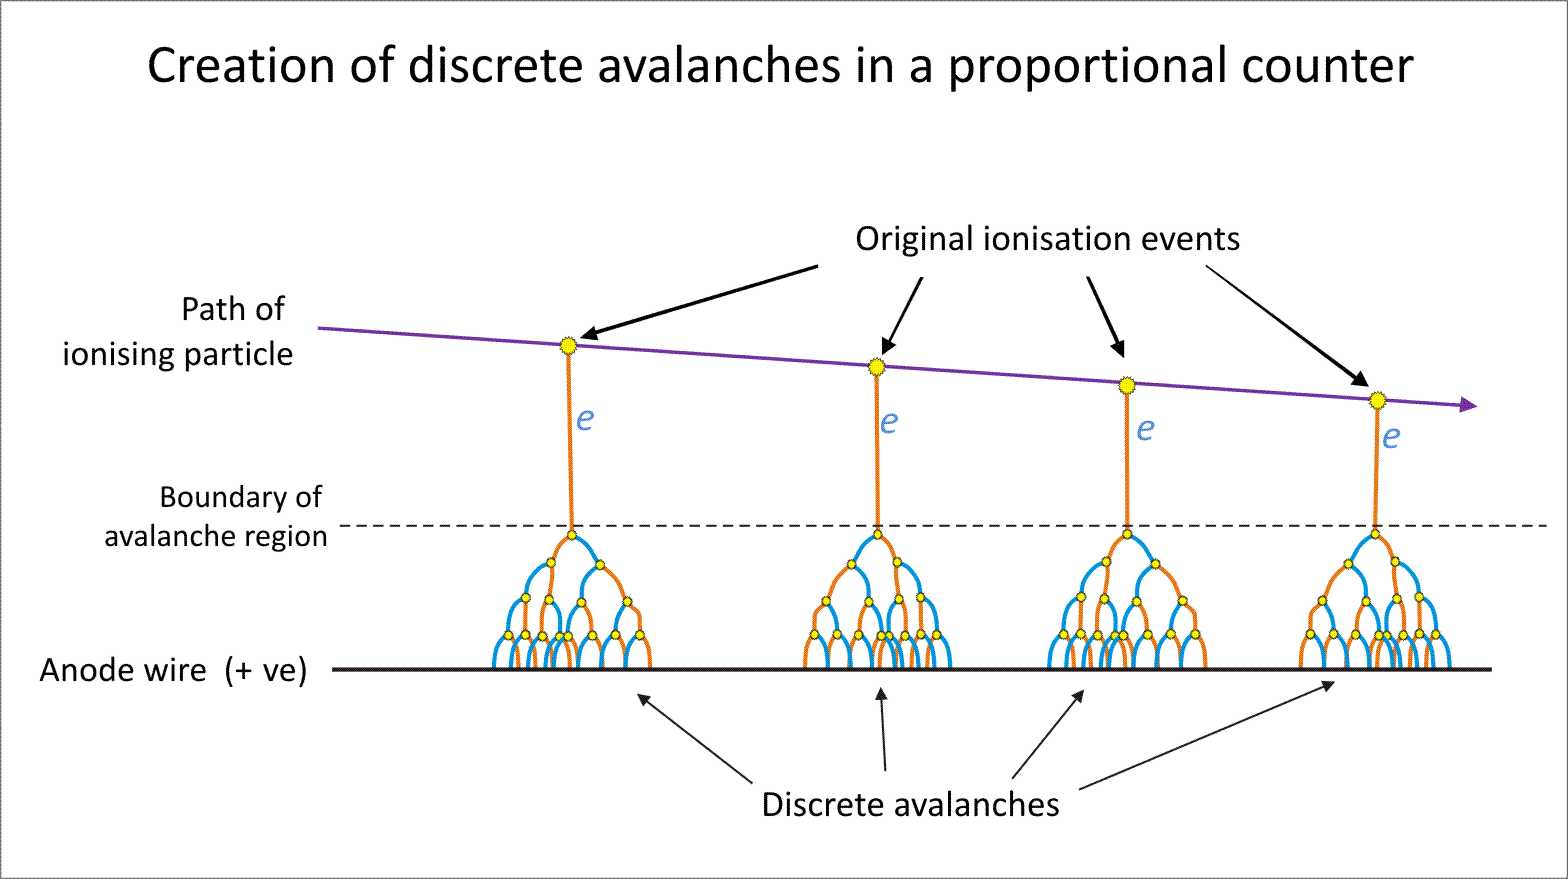
\includegraphics[width=0.8\textwidth]{Experimental_Aparatus/Proportional_counter.jpg}
  \caption{Principle of avalanche multiplication in a gas detector \cite{Dougsim2012}.}
  \label{fig:tpc_avalanche}
\end{figure}

If there is insufficient voltage to cause such an avalanche, instead the energy deposited at the electrodes are proportional to the number of initial ionisations alone, which is proportional energy deposited per unit length, $\text{d}E/\text{d}x$ and provides PID information. For this purpose, the voltage of the anodes are lowered and placed such that they can be in state called ''proportional mode''.

The ALICE TPC has a cylindrical geometry surrounding the ITS. It has an inner radius of 85 cm, an outer radius of 250 cm, and an overall length of 500 cm. A longitudinal electric field is applied over the cylinder, divided in the center by a cathode plate.  A voltage of 100 kV is applied between the center and endcaps, the resulting field strength within the detector volume is 400 V/cm. At the endcaps are Multi-Wire Proportional Chambers (MWPCs), arrays of anode wires operating in proportional mode. When a charged particle from the collision traverses the gas, electron-ion pairs will be created along its trajectory. Idealy, the field is longitudinal with minimal space charge distortions such that the electrons will be projected onto the endcaps, giving precise information about the (r, $\varphi$) coordinates of the trajectory. The drift velocity is carefully monitored using a laser system, which also detects inhomogeneities in the electric field. The laser system produces planes of tracks in the detector perpendicular to the electric field that make it easy to measure drift time as well as deviations caused by distortions. With a well determined drift velocity, the z coordinate is obtained by measuring the arrival time of the electrons. For the most frequently used TPC gas mixture – 85.7\% Ne, 9.5\% CO$_2$, and 4.8\% N$_2$ – this results in an average drift velocity of 2.65 cm/$\mu$s for the electrons, or an overall drift time of 94 $\mu$s for the longest drift distances. The endcaps are divided into 18 sectors, with four readout chambers each – two inner readout chambers (IROCs) and two outer readout chambers (OROCs). The wire density is higher for the IROCs as they are closer to the beam pipe, and the voltage applied is slightly lower. There are no anode wires between the sectors, resulting in gaps in the detector acceptance. The readout chambers have three layers of wires. The innermost wires are thin anode wires spaced 2.5 mm from each other. The middle layer consists of thicker cathode wires, where the ions released during avalanches are collected. The signal is read out from cathode pad planes, with a size in ($r,r\varphi$) space ranging from 4$\times$7.5 mm$^2$ in the IROCs to 6$\times$15 mm$^2$ in the outermost OROC sector. This results in a total number of 159 radial clusters \cite{Alme2010}.


The operation of the TPC is usually a delicate balance. If the voltage is too high in the normal operational mode, photons released in the de-excitation of gas ions may trigger additional avalanches that skew the initial signal. Another issue has to do with the recombination of ions and electrons at the electrodes, where gas atoms may again enter an excited and prolong the avalanche. To prevent this, a molecular component – usually CO$_2$ or an organic molecule – is added as a quencher to the gas. Unfortunately, at the high interaction rates delivered in Run 2, unexpected large space-charge distortions were observed at very specific regions of the TPC. They appeared at the boundaries between certain IROCs and deflect the ionization electrons towards these boundaries, leading to a bias in the measured space-point position and effectively decreasing the active readout area. It was suspected that insufficient insulation of some wires in this area could cause strong electric fields leading to amplification and therefore columns of ions drifting back from in between the readout chambers. After the TPC was brought to the surface at the beginning of LS2 indeed tips of anode wires sticking out of the ledges were found on all affected chambers near the expected radii~\cite{Schmidt2020}. A reduction of the distortions in the hot spots by a factor of about 4 was achieved with the special voltage settings in 2018 compared to 2015~. These space charge distortions are shown in Fig.~\ref{fig:tpc_distortion}.

\begin{figure}[htpb]
  \centering
  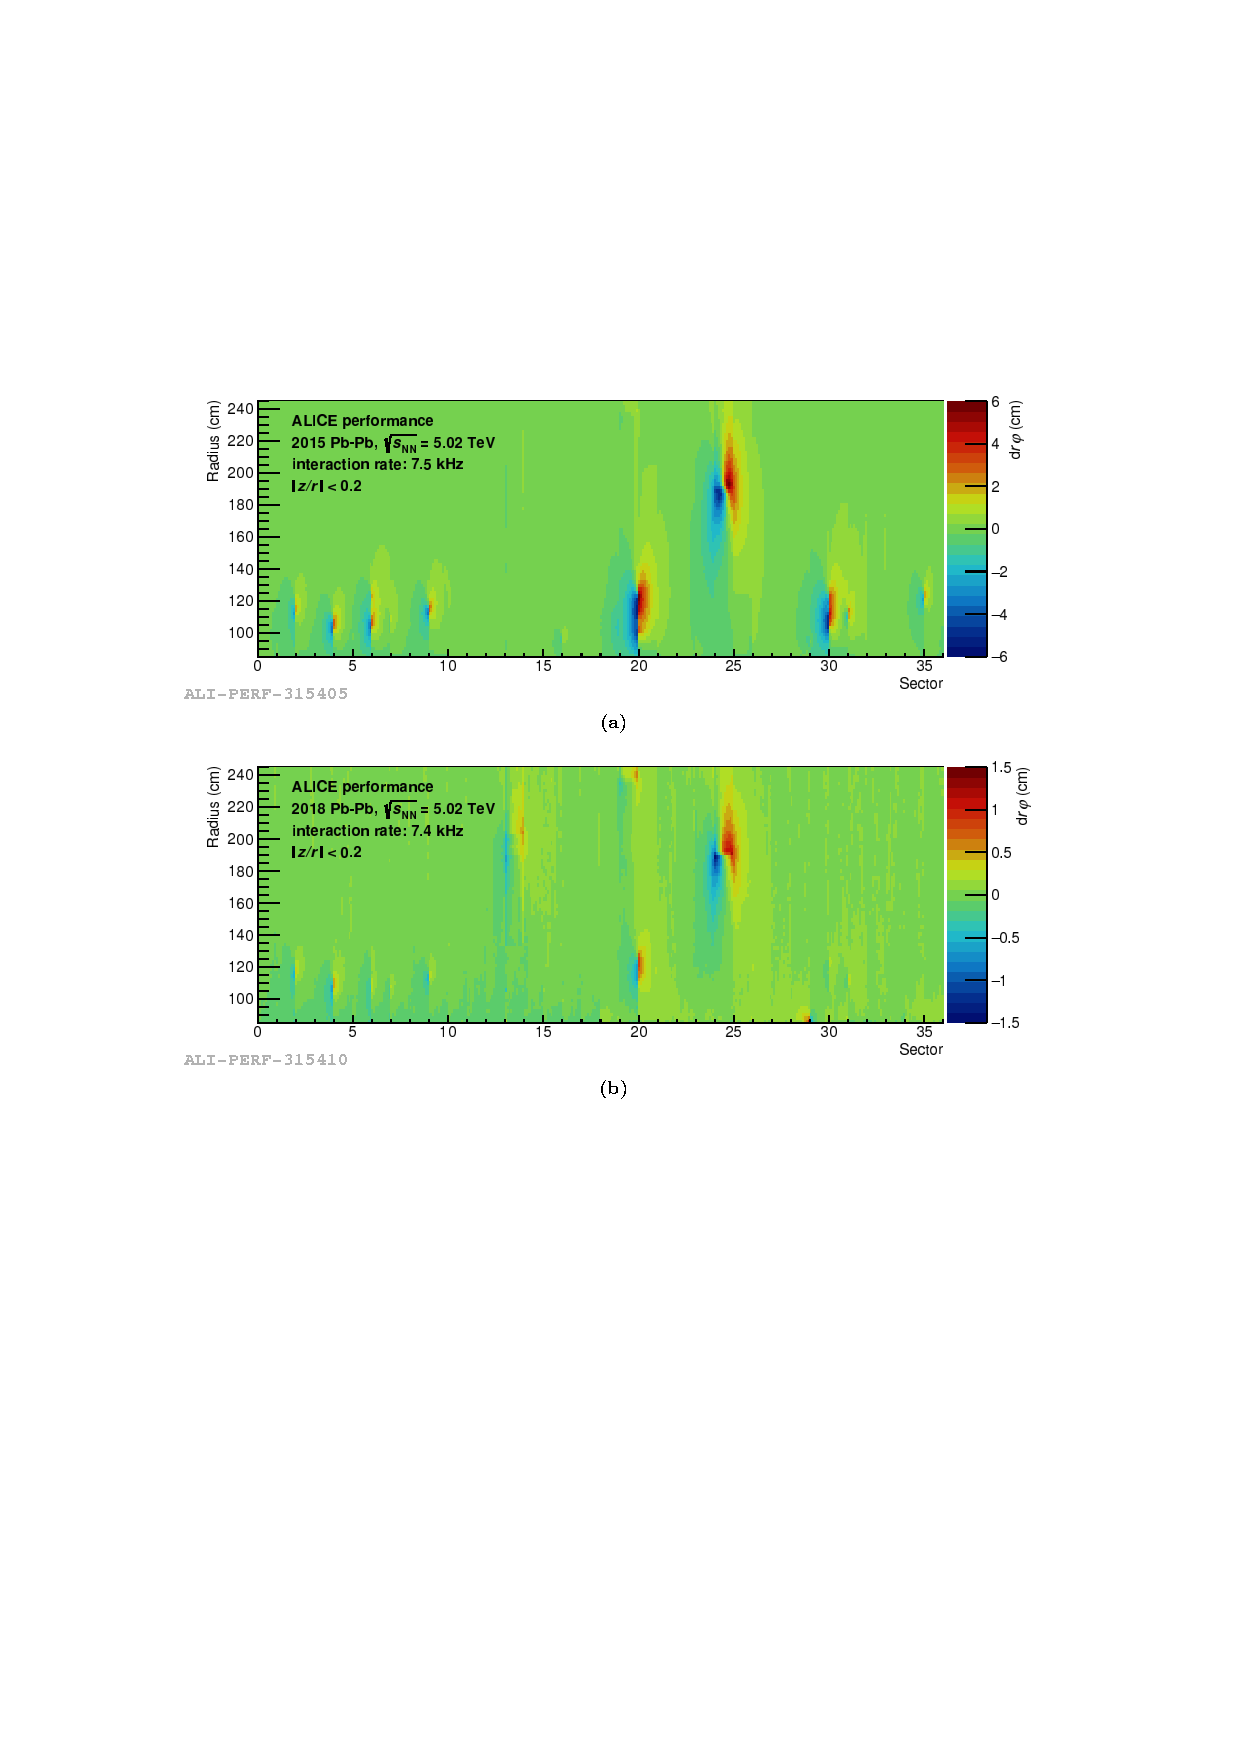
\includegraphics[width=0.8\textwidth]{Experimental_Aparatus/TPC_distortion.pdf}
  \caption{Measured space-charge distortions in $r\varphi$ near the central electrode are shown for Pb–Pb runs with high interaction rates in 2015 (upper plot) and 2018 (lower plot). For both runs the TPC was filled with argon. Note the different z-axis scales. \cite{Hellbar2019}}
  \label{fig:tpc_distortion}
\end{figure}


For the pp and \pPb data used in this analysis, the TPC was not read out or compromised for several runs. In order to maximize the statistics for the pp and \pPb, ITS-only tracking was used, a first in ALICE for two-particle correlations. The performance of ITS-only tracking vs. the standard TPC+ITS tracking is discussed in detail in Sec.~\ref{sec:tracking_published_comparision}.

\FloatBarrier
\subsection{Electromagnetic Calorimeter}
\label{sec:EMCal}

The Electromagnetic Calorimeter (EMCal) and Di-Jet Calorimeter (DCal) were mainly designed to measure high \pt objects. Originally, the calorimeter system in ALICE was proposed as layered lead-scintillator sampling calorimeter attached to wavelength shifting fibers for light collection \cite{Blau2020}, covering $107\textdegree$ in azimuth and  $|\eta| < 0.7$ in pseudorapidity. However, in order to enable the study of di-jet-events using full jets (rather than jets reconstructed with charged particle tracking alone), the calorimeter system was extended in 2010 to also include the DCal. The DCal is approximately opposite in $\varphi$ and uses design as the EMCal. The EMCal ond DCal are made up of 12288 and 5377 towers (also called cells), respectively. Each tower has a cross-sectional area approximately twice the Moli'ere radius of $\Delta\eta\times\Delta\varphi = 0.0143\times0.0143$ with a depth of 24.6cm that corresponds to approximately 20 radiation lengths. The calorimeters are organized into modules that are comprised $2\times2$ cells. These modules are further organized into 10 supermodules that are made up of up to $12\times24$ modules in the EMCal. Fig.~\ref{fig:emcal} (left) shows the EMCal made up of these supermodules, while (right) shows the various components that make up a single module.

\begin{figure}[htpb]
  \centering
  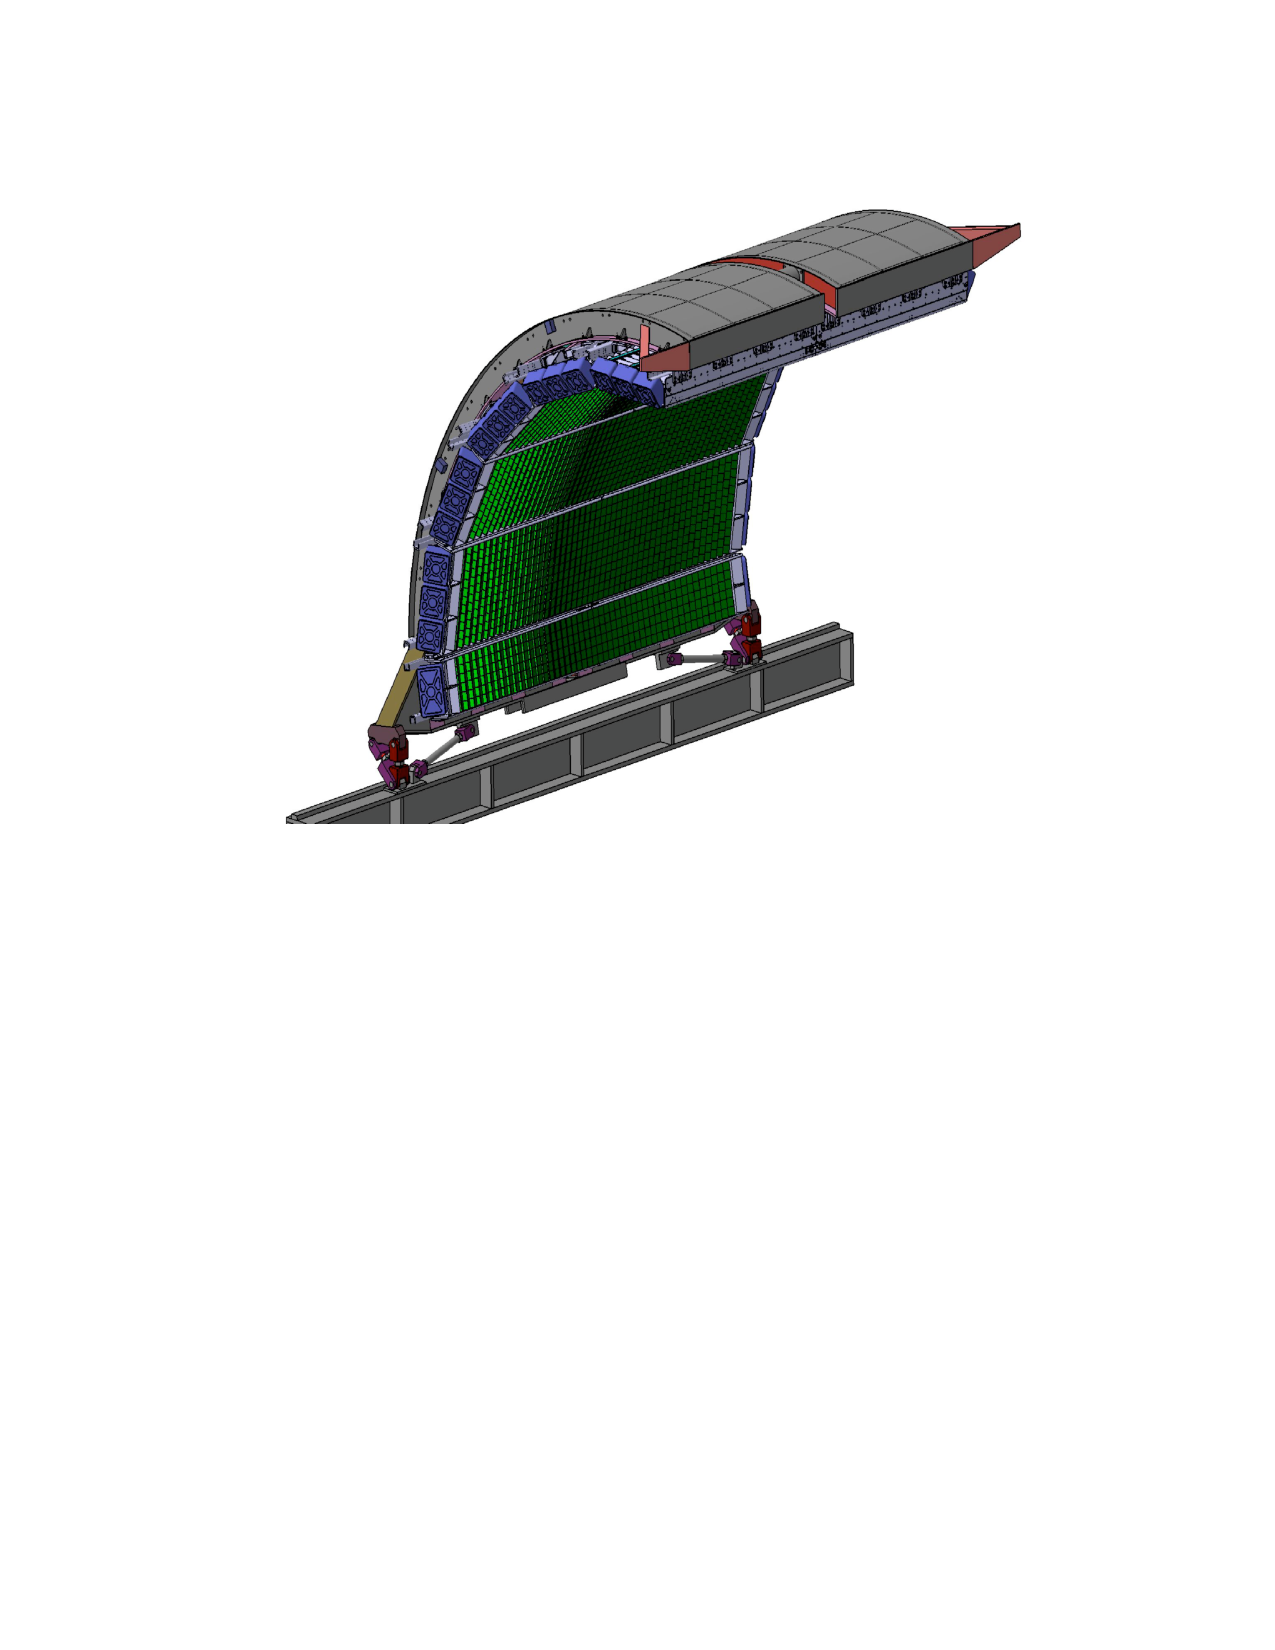
\includegraphics[width=0.45\textwidth]{Experimental_Aparatus/emcal.pdf}
  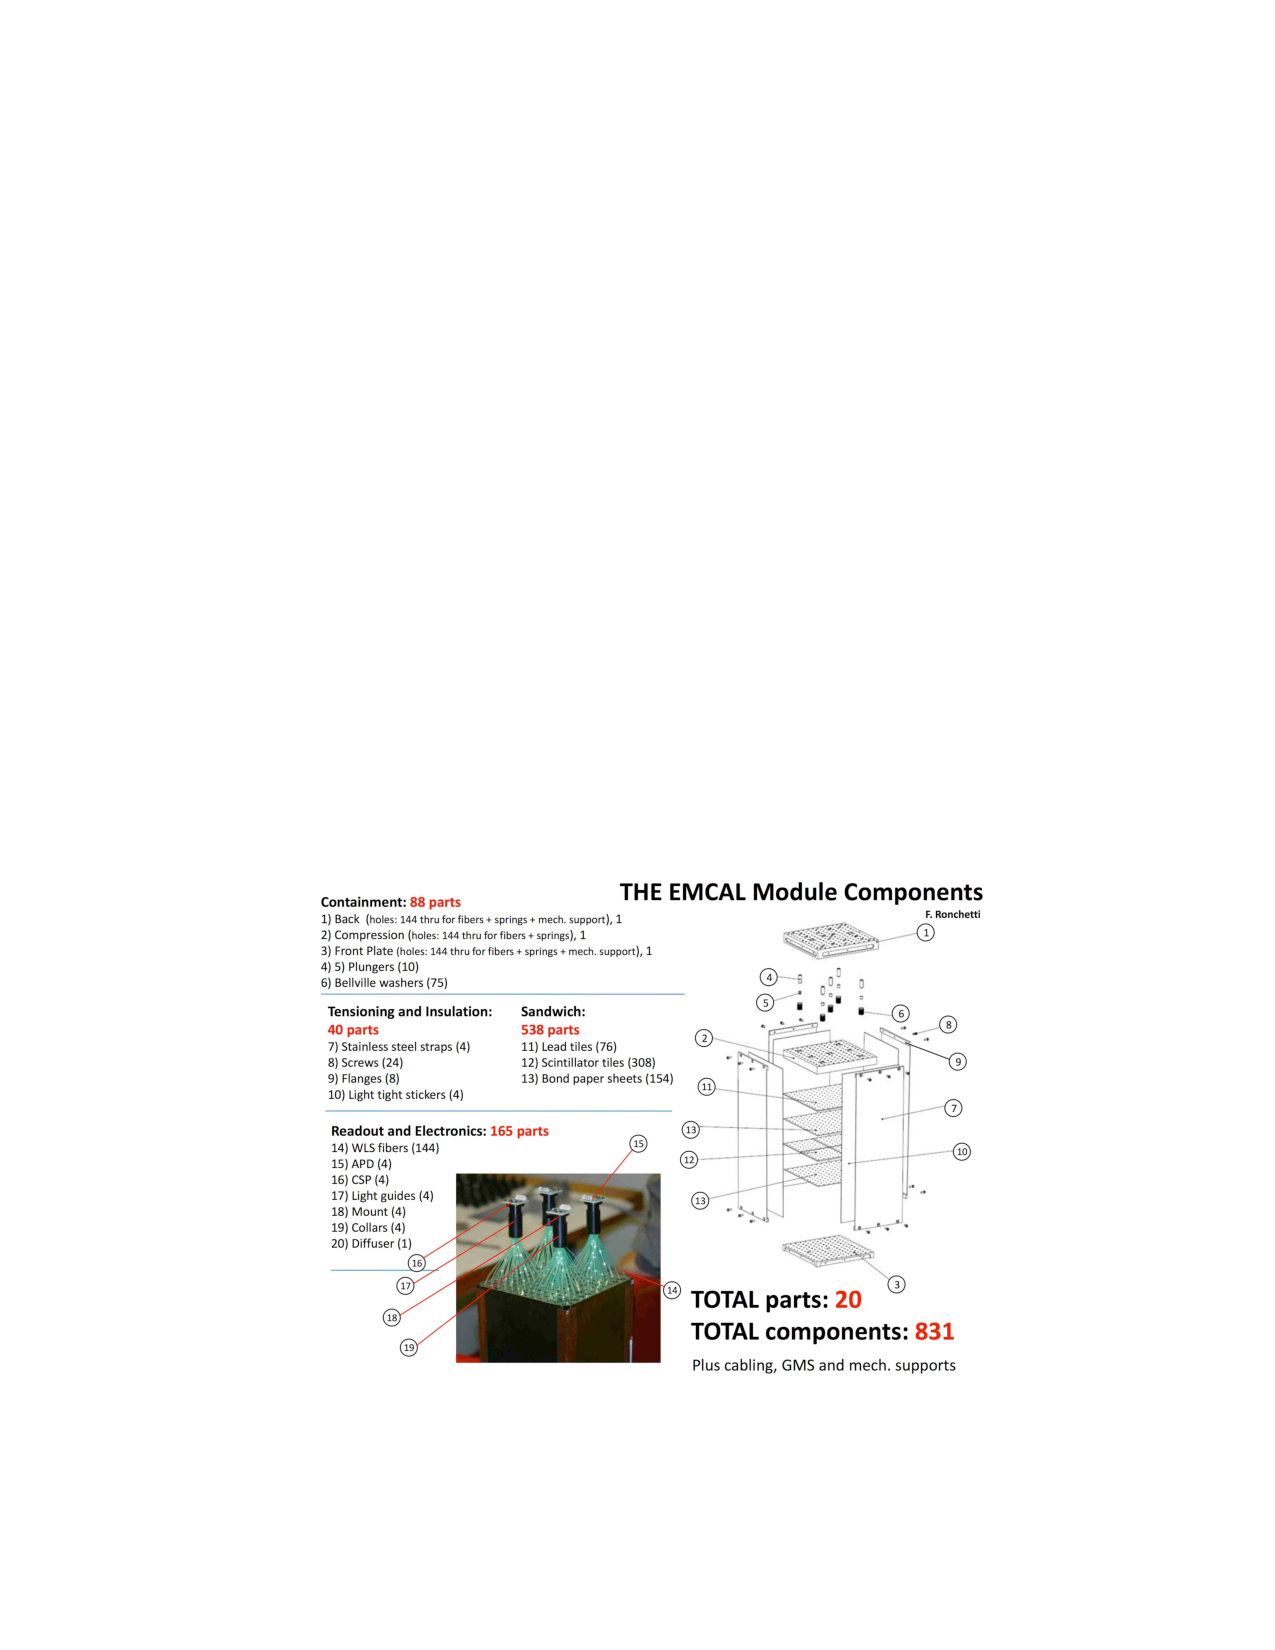
\includegraphics[width=0.45\textwidth]{Experimental_Aparatus/module.pdf}
  \caption{Left: The array of Super Modules shown in their installed positions on the support structure. Right: Exploded view drawing of EMCal module showing all components. Adapted from \cite{Bellwied2010}.}
  \label{fig:emcal}
\end{figure}


The wavelength shifting fibers are wired such that the scintillation light from each cell is read out by a $5\times5$ mm$^2$ avalanche photodiode. The relative energy resolution of the calorimeter is $\sigma/E = 1.7\% \oplus 11.3\%/\sqrt{E} \oplus 4.8\%/E$ for the energy range of interest for this analysis (roughly 10-50 \GeVc).


\subsection{Time of Flight Detector}
\label{sec:TOF}
The working principle of the TOF detector is to measure the time-of-flight from the interaction point of a particle in order to determine its velocity. Combined with the momentum information, one can extract the mass of the particle. The arrival time measurement is achieved by an array of Multi-gap Resistive-Plate Chambers (MRPCs). MRPCs are thin gaseous detector cells that have a high and uniform voltage applied to them~\cite{Aamodt:2008zz}. These are divided into two half-cells, each further divided into five smaller modules blocked by resistive glass plates. The field is sufficiently strong enough such that avalanche multiplication can occur, and thus a particle traversing the cell gives rise to a detectable signal. The glass plates block the avalanches, in order to reduce the time jitter, which scales with the propagation distance. The signals from each gap sum up to the total signal, and using multiple gaps increases the signal strength. The achieved time resolution is about 40 ps.

\begin{figure}[htpb]
  \centering
  \includegraphics[width=0.8\textwidth]{Experimental_Aparatus/LHC.png}
  \caption{Working principle of a TOF detector cell. A charged particle entering the cell will give rise to avalanches in the gas, which are blocked by glass plates mounted inside the cell. The resulting electrons will be picked up at the anode, which divides the cell into two half cells. Adapted from \cite{Adolfsson2020}.}
  \label{fig:TOF}
\end{figure}

The TOF detector has full azimuthal coverage and covers the pseudorapidity region of $|\eta| < 0.9$. The inner radius of the TOF is 370 cm with an active length of 741 cm. A total of 157,000 cells are arranged into 122$\times$13 cm$^2$ strips and put in 18$\times$5 modules (in ($\varphi,z$) space). The strips overlap each other to achieve full coverage within each module. In order to minimize the path length of particles coming from the collision, the modules are tilted so that each strip is facing the interaction point perpendicularly.

\section{Central Barrel Tracking}

A tracking algorithm must be used in order to reconstruct the particle tracks from hits in the detector. ALICE uses a Kalman filter algorithm. A Kalman filter uses a parametrisation of the track and optimises trajectories through the addition of additional space points. The algorithm is initiated with a seed, usually consisting of a few clusters in the TPC (the exception of course being the use of ITS-only tracking). An initial approximation of the track is made with the assumption that the track originates from the collision vertex, and is further extrapolated from hits in the SPD. The process is repeated by removing this constraint to account for the possibility that the track actually originates from a secondary vertex. The track information is continually improved by propagating the track \textit{inwards} and adding additional space points within 4 standard deviations of the best guess of the trajectory while accounting for multiple scattering and energy loss inside detector material. After each iteration, the parameters of the trajectory as well as the covariance matrix of the parametrisation are updated to improve accuracy. If more than one detector hit satisfies the selection criteria, multiple different propagations are tested, and the tracks with the lowest $\chi^2$ are selected at the end.

As the track is propagated from the outer edge of the TPC inwards, the tracking is further improved by adding hits from the ITS once the inner edge of the TPC is reached. For tracks where the primary vertex constraint has been lifted within the TPC, the same constraint is initially applied to ITS tracks, but repeated without the constraint as well: the higher precission of the ITS makes it possible to find secondary vertices that are much closer to the primary vertex. For tracks where the primary vertex constraint has already been lifted in the TPC, the ITS tracking is done once without imposing the constraint.

Once the track propagation is completed in both the TPC and the ITS, the Kalman filter algorithm is reversed by using track parameters the first procedure as an initial guess, but this time starts from the innermost layer of the ITS and propagates \textit{outwards}. The second iteration is applied in order to remove outliers from the initial track propagation. Once this iteration reaches the outer edge of the TPC, there is an option to incorporate hits from the other detector subsystems such as the Transition Radiation Detector (TRD), and eventually the TOF (as well as others), but this option is not used in this analysis. The main analysis of this thesis uses ITS-only tracking due to the space charge distortions of the time projection chamber discussed in Sec.~\ref{sec:TPC}. This results in tracks with fewer space points as input to the Kalman filter track reconstruction, but the performance was found to be comparable to the traditional ITS+TPC Hybrid tracking, Sec.~\ref{sec:tracking_published_comparision}.

\section{Triggering System}
\label{sec:trigger}


ALICE is capable of operating at an event rate of a few kHz. The LHC bunch crossing rate, however, is 40MHz. Even though not all bunch crossings result in a collision, an extensive triggering system is required to reduce the event rate and ensure all particles detected in an event are in fact from the same collision. This is also despite that fact that during pp collisions, the accelerator is actually tuned such that the luminosity at ALICE is $\mathcal{L}\approx 10^{30}-10^{31}\text{cm}^{-2}\text{s}^{-1}$, much lower than at ATLAS or CMS with a luminosity of $\mathcal{L}\approx 10^{30}-10^{31} \text{cm}^{-2}\text{s}^{-1}$. This reduces pile-up, but also the effective collision rate \cite{Wenninger:2668326}.

 The V0 and SPD detectors are the most important detector subsystems for triggering. The trigger input is handled by the Central Trigger Processor (CTP) that sends a command to all active detectors once it receives a successful trigger. There are three levels of triggers: L0, L1, and L2, and events are only accepted if the highest level, L2, triggers successively. The L0 trigger is simply synchronised with the LHC bunch crossing clock and includes the fastest inputs all processed within 1.2 $\mu$s after the collision. Additional inputs that take longer than 1.2$\mu$s and up to 6.5$\mu$s are handled by the L1 trigger. The L2 trigger then handles all the slower inputs, with the restriction that it must be completed before the TPC needs to be read out, less than $88\mu$s after the collision. 

The signals used by the trigger depend on the trigger configuration. One important configuration is minimum bias (MB), that selects against non-collisions. The MB trigger requires a hit in the both the V0A and V0C detectors. In order to reduce beam-gas events, additional requirements on the V0 timing information and on the correlation between the number of tracklets and clusters in the SPD are enforced. MB events are used in this analysis in the event mixing as well as in the ITS only tracking validation. Another trigger configuration is EG1, as well as EG2. These triggers require a hit in the EMCal up to a certain threshold before tracks can be read out for the event. For EG1, this threshold is 11 \GeVc, and 5\GeVc for EG2. 

Once the CTP receives a successful trigger, the CTP will begin a series of read-out operations for each active detector until eventually the trigger input is recorded locally at a Local Data Concentrator (LDC). During this processing, the read-out system will of course be busy, and a signal will be sent to the CTP that blocks triggering until the detectors are ready again. Some of the data from this read-out process is duplicated and sent to the High Level Trigger, where it is processed and decided wether the event should be stored permanently or rejected. This is the final triggering stage. If accepted, the data is compressed by rejecting irrelevant information and the remaining event data will be sent to Global Data Concentrators (GDCs) through the Data Acquisition (DAQ) system. The whole event is built from detector readouts in the GDCs, and is stored in first in Transient Data Storage. Some of the data is also processed online through data quality monitoring and detector algorithms to further reject bad quality events. For run two, the data quality monitoring is manual, and if there is a deterioration in quality, the shift leader may decide to stop a run until the problem is resolved. After all checks are passed, the data will be sent to the GRID for final storage, post-processing, and to be copied to tape. Because the data is so large and often inconvenient to pull for a single analysis, batches of analyses that need access to same dataset are grouped together in \textit{trains}. A train is then sent to the GRID to process a specific set of runs, and is the nominal way most analysis in ALICE are done. %often with at least one to two days between analysis iterations. The Berkeley group, however, takes a different approach to this method, discussed in more detail in \ref{sec:ntuples}.



\chapter{Data Anaysis}
\section{Analysis Summary}
This analysis uses the data collected during the \sqrtsNN{} = 5 TeV \pPb~run in 2013 and during the \sqrts{} = 5 TeV pp run in 2017. The EMCal trigger was used to select events with a high-momentum calorimeter cluster, a photon \pt range of {12--40 \GeVc}.%, equivalent to $x_{\mathrm{T}} = 2\pt/\sqrt{s_{\mathrm{NN}}}$ in the {0.006--0.012} range.  %The thresholds of the trigger corresponds to about {$\pt$ = 7 and 11 \GeVc} in the \pPb~data and about {5 \GeVc} in the pp data.

The signal for this analysis, is ''prompt'' photons, which include ''direct photons'' and ''fragmentation photons''. At leading order in perturbative QCD, the direct photons are produced in hard scattering processes such as quark-gluon Compton scattering ($qg\to q\gamma$) or quark-antiquark annihilation ($q\bar{q}\to g\gamma$), whereas the fragmentation photons are the product of the collinear fragmentation of a parton ($q\bar{q}(gg)\to \gamma + X$). At LHC energies, Compton scattering and gluon fusion $(gg\to  q\bar{q}\gamma)$ dominate due to the high-gluon density in the proton at small values of Bjorken-$x$. 

Beyond the simplistic leading order picture, the direct and fragmentation components have no physical meaning and cannot be factorized; the sum of their cross sections is the physical observable. For example, the separation between the NLO direct photons and LO fragmentation is arbitrary. However, it is still possible to simplify comparisons with theoretical calculations by applying an isolation criteria. The isolation variable used is the sum of the transverse momentum of the charged particles that are inside an angular cone of radius $R =\sqrt{(\Delta\phi)^{2} +(\Delta\eta)^{2}  } =0.4$ around the photon direction, after subtracting the underlying event. 

The main background for this analysis are photons from meson decays, which we will call ''decay photons'' or $\ydecay$. The  challenge faced in this measurement arises mainly from the small cross-section of the signal compared to that of the decay photon background (about 1$\%$ at {10 \GeVc} increasing to about 4$\%$ at {30 \GeVc}, according to next-to-leading order calculations~\cite{Arleo:2004gn}). 

This measurement exploits the difference between the electromagnetic shower profiles of prompt photons and of photon pairs from neutral-meson decays. The clusters that pass the isolation and shower shape selections isolated $\gamma$ candidates or ''\gammaiso candidates''. 

The main background in within the $\gammaiso$ candidate population are from multi-jet events where one jet typically contains a $\pi^{0}$ or $\eta$ that carries most of the jet energy and is misidentified as a photon because it decays into a photon pair that is collinear with respect to the EMCal cell granularity ($\Delta\eta\times\Delta\phi\approx$  14.3$\times$14.3 mrad$^{2}$), that is, the two photons are close enough to deposit most of their energy in the same cell and appear as a single shower. 

The signal purity of the $\gammaiso$ selection is measured by using the ''template-fit method'', in which the measured shower-shape distribution is fit with the sum of signal and background templates with the relative normalization as the single free parameter\footnote{Note that this is an standard way to estimate QCD background since at least the Tevatron days. The same exact method is used in the CMS $\gammaiso$ and $\gammaiso$--jet measurements in pp and PbPb data, for example in Refs.~\cite{Sirunyan:2018gro,Chatrchyan:2012gt}.}. The background template is mostly data-driven, calculated with an anti-isolated sideband requirement, but a MC-based correction is applied to account for estimated biases. The signal template is obtained from photon-jet simulation. The purity of our $\gammaiso$ selection is measured to be around 20$\%$ at {12 \GeVc} and increases to about 55$\%$ at {20 \GeVc} and above. 

Next, the angular correlation of the $\gammaiso$ candidates with charged particles is measured.  The {$\ydecay$--hadron} correlation function is measured by inverting the shower-shape cut to select merged-clusters from meson decays, and is called the \textit{Background Region} correlation function. Both the signal and background region photon-hadron correlations are corrected for geometrical pair acceptance effects using the mixed-event technique. Afterwards, the $\ydecay$--hadron correlation is normalized using the measured purity and subtracted from the normalized the main $\gammaiso$ candidate correlations in a process labelled "correlated background subtraction".

After this correlated background subtraction, the uncorrelated background, estimated by the zero-yield-at-minimum (ZYAM) method and checked by using a control region at large $|\eta^{\mathrm{hadron}}-\eta^{\gamma}|$ is subtracted from the main $\gammaiso$ candidate correlation function. Finally, the away-side of the resulting correlation function is integrated to determine the number of correlated hadrons per $\gammaiso$, i.e. to measure the conditional yield of hadrons. This analysis is performed with photons with $12<\pt <40~\GeVc$, and in intervals of charged particle \pt~and $\zt \equiv \pth/\ptgamma$. 

%We also present an $\gammaiso$--jet analysis. We reconstruct jets with the anti-$k_{\mathrm{T}}$ algorithm on tracks with {$0.15$ $<\pt < 15$ \GeVc} and $|\eta|<0.8$ as input. We select jets with {$\pt>$ 10 \GeVc} recoiling against the $\gammaiso$ candidate (with $|\phi^{\mathrm{jet}}-\phi^{\gamma}|>\pi/2$) and measure the angular correlations and momentum balance, and we also explore measurements sensitive to jet-flavor. To subtract the $\ydecay$--jet background arising from the impurity of our $\gammaiso$ candidate selection, we invert the shower-shape cut to select merged-clusters from meson decays and measure the corresponding background distributions, properly scaled by the purity of our $\gammaiso$ selection. We also subtract uncorrelated background, i.e correlations with jets produced by underlying event, by estimating it using event-mixing. The final $\gammaiso$--jet results are compared with $\pi^{0}$--jet correlations and \textsc{Pythia} photon+jet simulations at the reconstructed level and at particle level, i.e. after unfolding the jet detector smearing.

%The ratios of the p-Pb and pp distributions are compared to next-to-leading order perturbative quantum chromodynamic calculations with proton and nuclear parton distribution functions. While this measurement turns out to be dominated by statistical uncertainties, it still constrains the gluon densities in nuclei in the poorly explored low-$x$ and low-$Q^{2}$ region. This measurement also constitutes a benchmark for photon identification, background subtraction, and jet reconstruction for future measurements with larger data samples of proton-lead and lead-lead collisions. 

One of the novel aspects of this analysis is the use of ITS standalone tracking. This approach was developed in order to bypass the serious space-charge distortions that compromised the TPC during the high-luminosity \pPb~data taking in 2013\footnote{For details, see \url{https://alice.its.cern.ch/jira/browse/ATO-351}, \url{https://alice.its.cern.ch/jira/browse/PWGPP-349},
\url{https://alice.its.cern.ch/jira/browse/PWGPP-314}
}. Furthermore, the ITS-only tracking allowed the 2017 pp run to operate in the CALO mode that yielded a much larger sample than would have been possible otherwise. 

The performance of the ITS-standalone tracking (fake rate, efficiency and momentum smearing) was validated by measuring the charged particle spectrum and comparing it with published ALICE measurements at the same center-of-mass energy. These studies showed an agreement between the ITS-standalone measurement and the published data to within $\approx \pm 5\%$ of the corresponding published data for the range {$0.5<\pt<10$ \GeVc}, which is the relevant range in this analysis. 

One of the main considerations of the larger analysis strategy was to minimize the use of Monte Carlo simulations. By using an isolation variable constructed using only charged particles, the correlations between isolation and shower-shape variables due to the opening angle of neutral-meson decays has been reduced, at the expense of a slightly lower purity. In the template fit analysis, checks were performed that are independent of any input from simulations, suggesting the template fit is not sensitive to the detailed simulation of the exact shower-shape distributions. Moreover, the analysis measures per-trigger quantities such that there is no need to correct for the efficiency of the $\gammaiso$ selection. %While we use Monte Carlo simulations to construct the response matrices used in the unfolding of the detector response for jet measurements, these are validated with {\it in situ} calibrations of the jet energy scale. Therefore, detailed studies of multidimensional comparisons of data and simulations are not needed for this analysis, and are skipped in this note. 

While an effort was made to collect and use the largest data samples available by pioneering high-rate data taking with ITS+EMCal, the measurement turns out to be dominated by statistical uncertainties. Faced with this reality, efforts to reduce the systematic uncertainties of the measurement were tempered such that they are smaller than the statistical uncertainty.

\section{Datasets}
\label{sec:datasets}
The datasets used in this analysis include the high-luminosity runs of the 2013 \pPb~run (13d,e,f) and the 2017 pp run (17q) that were collected with EMCal triggers, which are listed in Table~\ref{tab:triggerstrings}.  

\begin{table}[h]
    \centering
    \caption{EMCal triggers used in this analysis.}
   \label{tab:triggerstrings}
   \begin{tabular*}{1.0\columnwidth}{@{\extracolsep{\fill}}ll@{}}
        \hline
        Dataset &  Trigger Strings\\
        \hline
        \pPb & CEMC7EG1-B-NOPF-CENTNOTRD, CEMC7EG2-B-NOPF-CENTNOTRD,\\
        \hline
        pp & CEMC7EG2-B-NOPF-CALO, CDMC7DG2-B-NOPF-CALO,\\ 
           & CEMC7EG2-B-NOPF-CENT,	CDMC7DG2-B-NOPF-CENT\\
        \hline
   \end{tabular*}
\end{table}


The EMCal gamma trigers (EG1, EG2, DG1, DG2) are based on the summed energy in 2$\times$2 adjacent tiles (a tile is composed of an EMCal module, 2$\times$2 adjacent cells). The trigger thresholds were 7 and 11 \GeVc~during the 2013 \pPb~run and {5 \GeVc} during the 2017 pp run. %The EMCal jet (EJ1, EJ2) triggers are based on a patch of 32 $\times$ 32 adjacent towers, corresponding to an area of approximately 0.2 rad was used. This jet patch trigger fired if an integrated patch energy of at least 10 GeV (low-energy trigger) or 20 GeV (high-energy trigger) was found.

Due to the 2-in-1 magnet design of the LHC, which requires the same magnetic rigidity for both colliding beams, the beams had different energies during the \pPb~run ({$E_{\mathrm{p}}$ = 4 TeV}, {$E_{\mathrm{Pb}} $= 4 TeV$\times$Z}, where $Z=82$ is the atomic number of lead). In the lead nucleus, the energy per nucleon was therefore  {$1.56$ TeV $= (Z/A) \times$ 4 TeV}, where $A =$ 208 is the nuclear
mass number of the lead isotope used. This energy asymmetry results in an average nucleon--nucleon center of mass collision energy of {$\sqrt{s_{\mathrm{NN}}}=5 $ TeV} and a rapidity boost of this frame by $\pm$0.465 units relative to the ALICE rest frame in the direction of proton beam. Around halfway through the 2013 \pPb~run, the beam directions were flipped, yielding similar integrated luminosities in both beam configurations. %Following an established convention, we report pseudorapidity in the nucleon-nucleon collision frame, $\eta^{*}$, with a positive (negative) pseudorapidity corresponding to production in the downstream proton (downstream nuclear) beam direction. Therefore, a massless particle emitted at $\eta_{\mathrm{cm}}=0$ in the nucleon-nucleon center-of-mass frame will be detected at $\eta_{\mathrm{lab}}=$+0.465 in the laboratory frame.  

%%%%%%%%%%%%%%%%%%%%%%%%%%%%%%%%%%%%%
During the 2013 \pPb~run period, the TPC suffered from space-charge distortions\footnote{For more information on the problems with space-charge distortions due to high-luminosity in \pPb~run, see: https://alice.its.cern.ch/jira/browse/PWGPP-314.} that affect tracking, leading to a very drastic drop in efficiency for tracks with $\pt> 4$ \GeVc. We bypass this issue by using ITS-only tracking as detailed in Section~\ref{sec:tracking}.
For the 2017 pp data, the TPC was also inactive due to the high luminosity of the runs considered in this analysis. We use the 17q period, during which all six layers of the ITS were active.

The average number of inelastic collisions per bunch crossing, $\mu$, is 0.020--0.060 for the 2013 \pPb~data set and in the range 0.015--0.045 for the 2017 pp dataset~\footnote{This information can be found in \url{http://aliqaevs.web.cern.ch/aliqaevs/data/2013/LHC13d/pass4/global_properties.pdf} and \url{http://aliqaevs.web.cern.ch/aliqaevs/data/2017/LHC17q/cpass1_pass1/global_properties.pdf}}.% Thus, one expects an in-time pileup, i.e. multiple collisions in the same bunch crossing at the level of less than 1$\%$ (given by the Poisson probability of $P(n>1) = 1-P(n=0) = e^{-\mu})$. 

%Figure~\ref{fig:RejectionFactorpPb} shows the rejection factor of the EMCal gamma triggers. The curves already reached a plateau for clusters with $\pt=12$ \GeVc, which is the minimum $\pt$ used in this analysis. 

%%\begin{figure}[h]
%\center
%\includegraphics[width=0.6\textwidth]{Datasets/RejectionFactorpPb2013}
%\caption{Rejection factor curves for the 2013 p-Pb period (13def). Source: Ref.~\cite{Erwann}.}
%\label{fig:RejectionFactorpPb}
%\end{figure}


%The total integrated luminosity of the 2013 p-Pb sample is about {4.6 nb$^{-1}$} {($\times$ $A$ = 967 nb$^{-1}$ pp equivalent luminosity)} and about {300 nb$^{-1}$} for the 2017 pp sample. Note that the DCal increases the geometrical acceptance for photons by roughly a factor of 1.3; therefore, comparable statistics of high-$\pt$ photons are expected for pp and p-Pb data.~\footnote{This is the first hard-probes analysis in ALICE that has similar statistics in the reference pp data at the same center-of-mass energy, and thus does not need to rely on extrapolations.}



\section{Monte Carlo simulations}
\label{sec:mcsimulations}
We use Monte Carlo (MC) simulations to obtain the signal shower-shape distributions for the template fits (section~\ref{sec:purity}) and to study tracking performance (section~\ref{sec:tracking}).

The simulations of hard processes are based on the \textsc{Pythia} event generator. In \textsc{Pythia}, the signal events are included via $2\to2$ matrix elements with $gq\to\gamma q$ and $q\bar{q}\to\gamma g$ hard scatterings, defined at the leading order, followed by the leading-logarithm approximation of the partonic shower. The soft underlying events in pp collisions as well as fragmentation are included with the default \textsc{Pythia} models. 

For the simulation of \pPb~events, the pp samples are embedded into \pPb~inelastic events generated with \textsc{DPMJET}. The boost of $\Delta y=+0.465$ in the direction of the proton beam is reproduced. % to reproduce the experimentally measured global \pPb~event properties. 

% Table~\ref{tab:MCsamples} shows the MC simulations used in this analysis. Each sample is simulated with the detector configuration appropriate for the runs used in this analysis. 

% \begin{table}[h]
%    \centering
%    \caption{Monte Carlo simulations used in this analysis.}
%    \label{tab:MCsamples}
%    \begin{tabular*}{1.0\columnwidth}{@{\extracolsep{\fill}}llcc@{}}
%     \hline
%         Name  & Configuration & JIRA ticket link \\
%         \hline        
%  17g6a1	 &\pPb, 5 TeV, \textsc{Pythia8} Gamma-Jet +DPMJET anchored to 13d,e,f& \href{https://alice.its.cern.ch/jira/browse/ALIROOT-7271}{ALIROOT-7271}\\
%  17g6a3	 &\pPb, 5 TeV, \textsc{Pythia8} Jet-Jet +\textsc{DPMJET} anchored to 13def& \href{https://alice.its.cern.ch/jira/browse/ALIROOT-7271}{ALIROOT-7271}\\
%   13b2    &\pPb, 5 TeV, \textsc{Dpmjet} anchored to LHC13b,c & \href{https://alimonitor.cern.ch/productions/3996/tag.html}{39374}\\
%  18b10a(b)\_calo	 &pp 5 TeV, \textsc{Pythia8} Gamma-Jet anchored to 17p/q& \href{https://alice.its.cern.ch/jira/browse/ALIROOT-7692}{ALIROOT-7692}\\
%  18l2a(b)     &pp 5 TeV, \textsc{Pythia8} Jet-Jet anchored to 17p/q& \href{https://alice.its.cern.ch/jira/browse/ALIROOT-8144}{ALIROOT-8144}\\
   
%                  \hline
%    \end{tabular*}
% \end{table}


\section{Event Selection}
\label{sec:eventselection}
The following event selection criteria is used to ensure good event quality and uniform acceptance:
\begin{itemize}
\item Run passes QA for EMCal and ITS (the selected runs are listed in Table~\ref{tab:datasets}).
\item At least one EMCal cluster with $\pt>12$ \GeVc.
\item Selected at least one of the EMCal triggers (logical OR of the trigger strings listed in Table~\ref{tab:triggerstrings}).  %(low and high thresholds).
\item Valid vertex ($|z|\neq0.0$) and $|z|<10$ cm 
%\item Pileup rejection (\textsc{IsPileupFromSPD}(5, 0.8)=False).
\end{itemize}

Where the EMCal is mentioned, we use the same criteria on the DCal (used in the 17q dataset). We use EMCal in text for brevity.
The number of events that pass our selection in each sample is shown in Table~\ref{tab:eventsselected}. We report the events selected for each trigger separately, as well as the logical OR combination. In \pPb~events, the number of events is dominated by the EG1 trigger (11 \GeVc~thrshold), and by the EG2 trigger (5 \GeVc) in pp collisions. 

\begin{table}[h]
   \centering
   \caption{Number of events that passed our full event selection for each of data taking period used in this analysis. The numbers are also shown separately for EG1 (DG1) and EG2 (DG2) triggers.}
   \label{tab:eventsselected}
   \begin{tabular*}{1.0\columnwidth}{@{\extracolsep{\fill}}llll@{}}
    \hline
    Dataset &  	N$^{\mathrm{EG1||EG2}}$ &	N$^{\mathrm{EG1}}$ & N$^{\mathrm{EG2}}$\\
    \hline
    13d &	134024 & 133326 & 12528\\
    13e &	198108 & 196745 & 22409\\
    13f &   340607 & 338198 & 38353\\
    13f\_new & 241870 & 240074 & 30310\\
%    Dataset &  	N$^{\mathrm{EG1||EG2||EJ1||EJ2}}$ &	N$^{\mathrm{EG1}}$ & N$^{\mathrm{EG2}}$ &	N$^{\mathrm{EJ1}}$  &	N$^{\mathrm{EJ2}}$ \\
%    \hline
%    13d &	173583 & 133326 & 12528 & 122168 & 20917\\
%    13e &	206833 & 196745 & 22409 & 167651 & 3063\\
%    13f &   365775 & 347684 & 40133 & 296144 & 6501\\
%    13f\_new & 252738 & 240074 & 30310 & 204298 & 5110\\
    \hline
    Dataset &	N$^{\mathrm{EG2 || DG2}}$ &		N$^{\mathrm{EG2}}$ & N$^{\mathrm{DG2}}$\\
    \hline

    17q & 406934 & 301086 & 119498 \\
 
    \hline
   \end{tabular*}
\end{table}

\section{Calorimeter cluster reconstruction}
\label{sec:clusterselection}
\subsection{Definition}
EMCal clusters are formed by a clustering algorithm that combines signals from adjacent towers. We use calorimeter clusters defined with the ``V1'' algorithm. This algorithm starts from a ``seed" cell, found from a local-maximum scan, and adds ``neighbor" cells to the cluster if they are above a given threshold. The cluster definition is exclusive, i.e. once a cell is assigned to a cluster, it is not considered for other clusters. The minimum energy for the seed and neighbor were set to 500 and 100 MeV respectively; these values are several times larger than the standard deviation of the electronic noise\footnote{Some photon analysis use a 50 MeV threshold, but 100 MeV has been found to improve cell time measurements. The 100 MeV threshold has been used for example in Ref~\cite{Acharya:2017tlv}.}.

\subsection{Corrections}
We apply several corrections at the cell level, implemented within the ``EMCal Correction Framework,"\footnote{\url{http://alidoc.cern.ch/AliPhysics/master/_r_e_a_d_m_eemc_corrections.html} } before the clustering algorithm is run over the data and simulations. The following corrections are applied: 
\begin{itemize}
\item ``\textsc{CellEnergy}"\\
This performs an energy calibration of cells, with coefficients obtained with $\pi^{0}\to\gamma\gamma$ mass measurements.
\item ``\textsc{CellBadChannel}''\\
This removes cells that declared hot or dead for a given run period. 
\item ``\textsc{CellTimeCalib}"\\
This correction applies constant offsets, which are arbitrary, to the cell time measurements to minimize the spread among cells. 
\item ``\textsc{CellEmulateCrosstalk}''. \\
This correction, described in detail in Ref~\cite{CrossTalk}, modifies the simulated cell energies to emulate the cell cross-talk that has been observed in data. This is applied to all the simulations described in Table~\ref{tab:MCsamples}. 
\end{itemize}

\subsection{Selection}
The following selection is applied on the resulting clusters\footnote{This event selection also closely follows previous and concurrent isolated-photon spectra analyses in pp and \pPb~ data.}:

\begin{itemize}
\item Cluster $\pt$ cut:  $12< \pt < 40$ \GeVc.
\item Cluster pseudorapidity: $|\eta| <0.67$\\
The cluster pseudorapidity is corrected for the position of the primary interaction vertex. 
\item Number of cells cut: $N_{\mathrm{cell}}\geq2$\\
This requirement removes clusters that are likely dominated by noise. 
\item Exoticity cut: $E_{\mathrm{cross}}/E_{\mathrm{cluster}}$ $> 5\%$\\
We remove ``exotic'' or ``spiky'' clusters likely coming from slow neutrons or highly-ionizing particles hitting the avalanche photo-diode of a cell by a requirement on the ratio of the summed energy around the leading cell to the total cluster energy.
\item Cluster time cut:  $|t|<20$ [ns]\\
We require a cluster time measurement of $|t|<$ 20 ns to remove out-of-bunch pileup. 
\item Number of local maxima cut: $N_{LM}<$ 3\\
This cuts suppresses background and improves the MC simulation description of the background~\cite{Acharya:2019jkx}.  
\item Distance seed-cell to bad-channel$\geq 1$ cells.
\end{itemize}

Figures~\ref{ClusterCutFlow_pPb} and~\ref{ClusterCutFlow_pp} show the distribution of the variables used in the cluster selection and the effect of sequential selection (``cut flow") for the \pPb~and pp data respectively. Table~\ref{tab:photonCutFlow} shows a summary of the effect of sequential selection on the number of selected clusters in both pp and \pPb~data. 

\begin{figure}[h]
\center
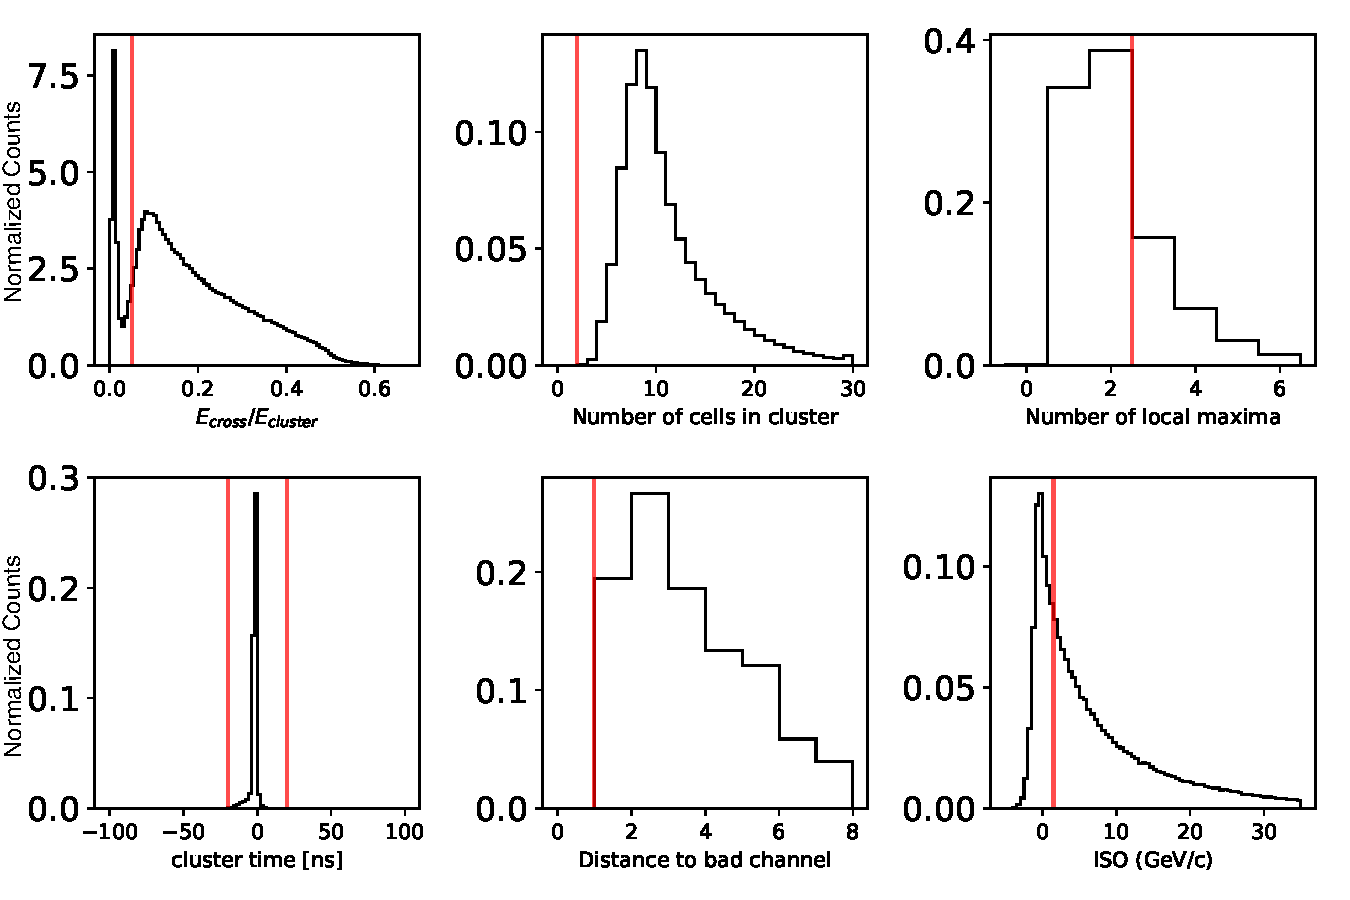
\includegraphics[width=0.95\textwidth]{Data_Analysis/EventAndClusterSelection/ClusterCutFlow_dataset_Skimmed_13def}
\caption{Distribution of variables used in the cluster selection of \pPb~data. The red vertical lines represent the cuts used. The cluster cuts get applied sequentially, i.e. the clusters cut with a given variable do not appear in the next.}
\label{ClusterCutFlow_pPb}
\end{figure}


\begin{figure}[h]
\center
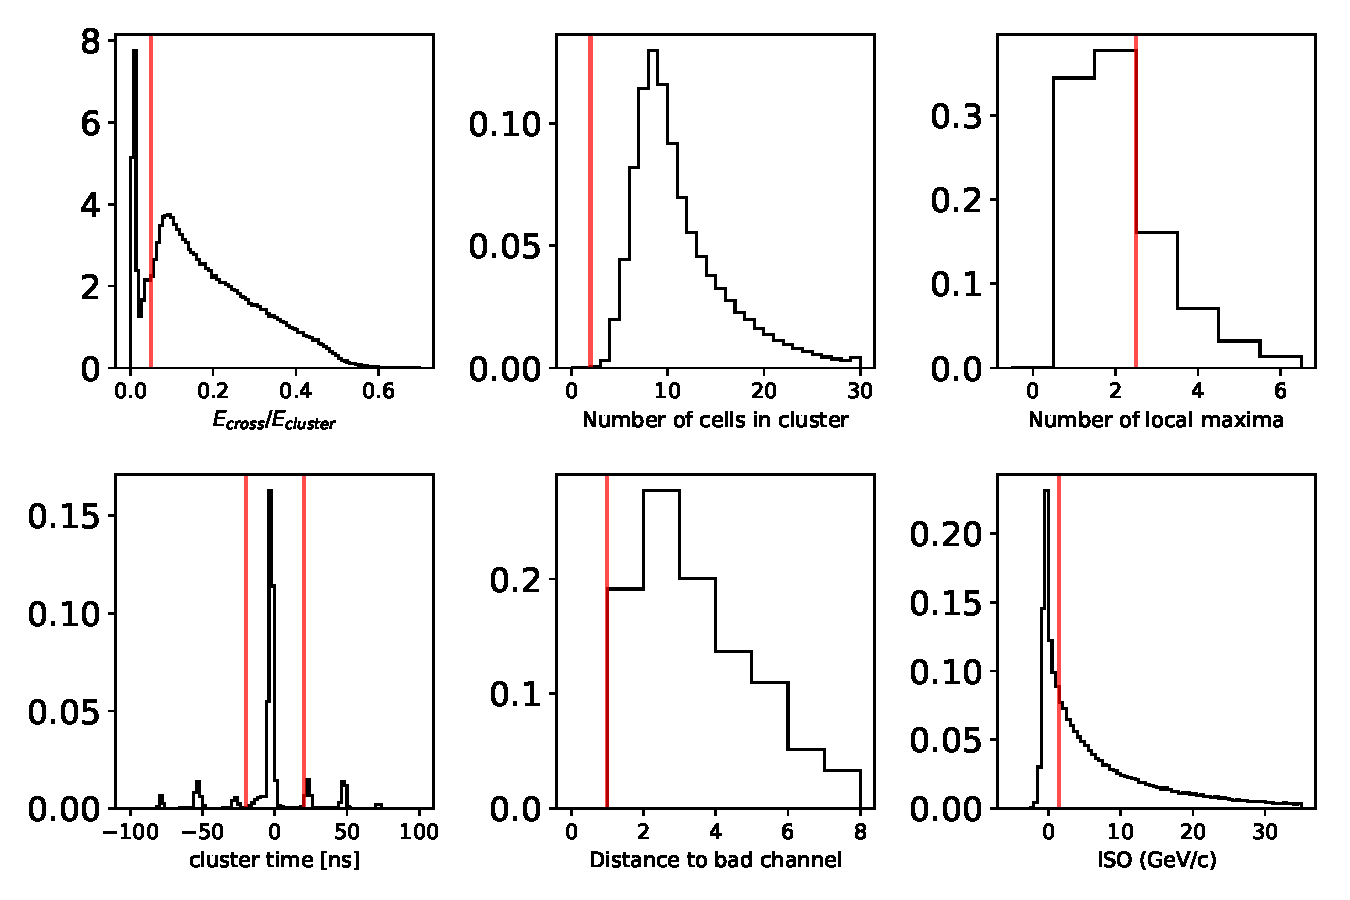
\includegraphics[width=.95\textwidth]{Data_Analysis/EventAndClusterSelection/ClusterCutFlow_dataset_Skimmed_17q}
\caption{Distribution of variables used in the cluster selection in pp data. The red vertical lines represent the cuts used. The cluster cuts get applied sequentially, i.e. the clusters cut with a given variable do not appear in the next.}
\label{ClusterCutFlow_pp}
\end{figure}


\begin{table}[h]
   \centering
   \caption{Number of clusters, with  $12<\pt<40$ \GeVc, that pass our selection in 2013 \pPb~and 2017 pp data.}
   \label{tab:photonCutFlow}
   \begin{tabular*}{1.0\columnwidth}{@{\extracolsep{\fill}}lcc@{}}
    \hline
       Selection  &  \pPb~ data & pp data  \\
       \hline
       $|\eta| < 0.67$& 714834 & 385220  \\
      $E_{\mathrm{cross}}/E_{\mathrm{cluster}}$ $> 5\%$ & 613560 & 323750   \\
       $N_{\mathrm{cell}}$ $\geq 2$   &613560& 323750       \\
              $N_{LM}<$ 3 & 443102&231490 \\
       $|t|<20$ [ns] &441639 & 171470  \\ 
       Distance-to-bad channel $\geq 1$ &441639  &171470  \\ 
       $\iso<$  1.5~\GeVc & 137895  & 58638 \\ 
       0.1 $< \sigma^2_{\textrm{long}}<$  0.3  & 40027 & 16628  \\ 
       \hline
	   %Total clusters passing $\gammaiso$ selection & 38415  & 16,586 %\\ 
       %\hline
   \end{tabular*}
\end{table}

\FloatBarrier

\section{Isolated Prompt Photon Selection} 
\label{sec:photons}

A key challenge of this measurement is the relatively small cross section of prompt photons compared to decay photons. In order to reduce the background of decay photons, and to identify prompt photons, a combination of isolation and electromagnetic shower profile selections are made. Photons are observed in their final state as an reconstructed cluster in the calorimeter. Clusters are obtained by grouping all adjacent cells with common sides whose energy is above {100 MeV}, starting from a seed cell with at least {500 MeV}. Furthermore, a cluster must contain at least two cells to remove single-cell electronic noise fluctuations. Clusters are required to have a minimum \pt of \ptgamma $\geq 12$ \GeVc. The time of the highest-energy cell in the clusters relative to the main bunch crossing must satisfy $\Delta t < 20$ ns to reduce out-of-bunch pileup. In order to limit spurious signals caused by particles hitting the EMCal APDs, clusters are required to have $E_{\mathrm{cross}}/E_{\mathrm{cluster}}>0.05$, where $E_{\mathrm{cross}}$ is the sum of the energy in the cells adjacent to, but not including, the leading cell, and $E_{\mathrm{cluster}}$ is the total energy of the entire cluster. The number of local maxima in the cluster is required to be less than three to reduce hadronic background. To select against photons from neutar-meson decays or fragmentation processes, a shower profile selection and isolation requirement are applied to these clusters. 

%Also included in the definition of direct photons are thermal photons. These photons are produced as thermal radiation emitted by the quark gluon plasma. Thermal photons dominate the direct photon spectrum at low \pt, and at energies much lower than the photons of interest in this measurement (Section \ref{sec:photon_selection}).

\subsection{Shower Profile Selection}
The primary background for this measurement are photons from the 2-body decay channel of neutral mesons $\pizero$'s. A \pizero~with a higher \pt will decay  with a smaller opening angle between the two decay photons. As the opening angle becomes smaller, the electromagnetic showers from the decay photons get closer together in the EMCal until they begin to overlap. For this reason, photons from $\pi^0$ decays begin to merge into a single cluster in the EMCal above approximately 6~\GeVc. This cluster, made up of two showers from decay photons, will therefore tend to have a more elongated shower profile than a cluster resulting from a single, ideally prompt, photon. Thus, in order reject clusters produced by two photons from a meson decay, and select clusters from single photons, we select clusters using variables that encode the shape of the calorimeter shower. 

A variable that encodes the shape of a cluster's electromagnetic shower profile for this purpose is \lambdasquare. 
The \lambdasquare~variable is defined as the square of the larger eigenvalue of the energy distribution in the $\eta$--$\varphi$ plane:
\begin{equation}
\lambdasquare = (\sigma^{2}_{\varphi\varphi} + \sigma^{2}_{\eta\eta})/2 + \sqrt{(\sigma^{2}_{\varphi\varphi} - \sigma^{2}_{\eta\eta})/4 + \sigma^{2}_{\varphi\eta}},
\end{equation}

where $\sigma^{2}_{ij} = \langle ij \rangle - \langle i \rangle\langle j \rangle$ are the covariance matrix elements; the integers $i,j$ are cell indices in $\eta$ and  $\varphi$ axes; $\langle ij \rangle$ and $\langle i\rangle$, $\langle j\rangle$ are the second and the first moments of the cluster position cell. The position is weighted by $\mathrm{max}\left(\log(E_{\mathrm{cell}}/E_{\mathrm{cluster}}) - w_{0},0\right).$ Following previous work~\cite{Acharya:2018dqe}, the cutoff in the log-weighting is chosen to be $w_{0}=-4.5$. Cells that contain less than {$e^{-4.5} =$ 1.1$\%$} of the total cluster energy are not considered in the $\lambdasquare$ calculation. Thus, $\lambdasquare$ discriminates between clusters belonging to single photons, having a $\lambdasquare$ distribution which is narrow and symmetric, and merged photons from neutral meson decays, which are asymmetric and have a distribution dominated by a long tail towards higher values. 

Most single-photon clusters yield $\lambdasquare\approx 0.25$, as shown in Figure \ref{fig:TemplateFit} where the signal is displayed in blue. Consequently, a cluster selection of $\lambdasquare<0.30$ is applied irrespective of \pt. Simulations indicate this results in a signal efficiency of about 90$\%$ with no significant \pt~dependence.


% The $\lambdasquare$ variable is the weighted root-mean-square of the shower energy along the major ellipse axis, and thus clusters with a symmetric shower profile will trend towards smaller values of $\lambdasquare$. $\lambdasquare$ is defined according to~Ref.~\cite{Abelev:2014ffa} as:
% \begin{equation}
% \lambdasquare = \frac{s_{\eta\eta}+ s_{\phi\varphi}}{2} + \sqrt{   \frac{(s_{\eta\eta} - s_{\phi\varphi})^{2}}{4} + s^{2}_{\eta\varphi}         },
% \end{equation}
% where $s_{ij} = \langle ij \rangle - \langle i \rangle\langle j \rangle$ are the covariance matrix elements; the $i,j$ are cell indices in $\eta$ and  $\varphi$ axes; $\langle ij \rangle$ and $\langle i\rangle$, $\langle j\rangle$ are the second and the first moments of the cluster position cell weighted as follows:
% \begin{equation}
% \mathrm{weight} = \mathrm{max}\left(\log(E_{\mathrm{cell}}/E_{\mathrm{cluster}}), w_{0}\right). 
% \end{equation}

% Following previous studies~\cite{Acharya:2018dqe}, we chose the cutoff in the log-weighting as $w_{0}=-4.5$, which means that cells that contain less than {$e^{-4.5} =$ 1.1$\%$} of the total cluster energy are not considered in the $\lambdasquare$ calculation.

Fig.~\ref{fig:sigma_long_shapes} shows an example of a cluster with an elongated shower profile with a large \lambdasquare, and a narrow, symmetric cluster with a smaller \lambdasquare.

\begin{figure}[htpb]
  \centering
  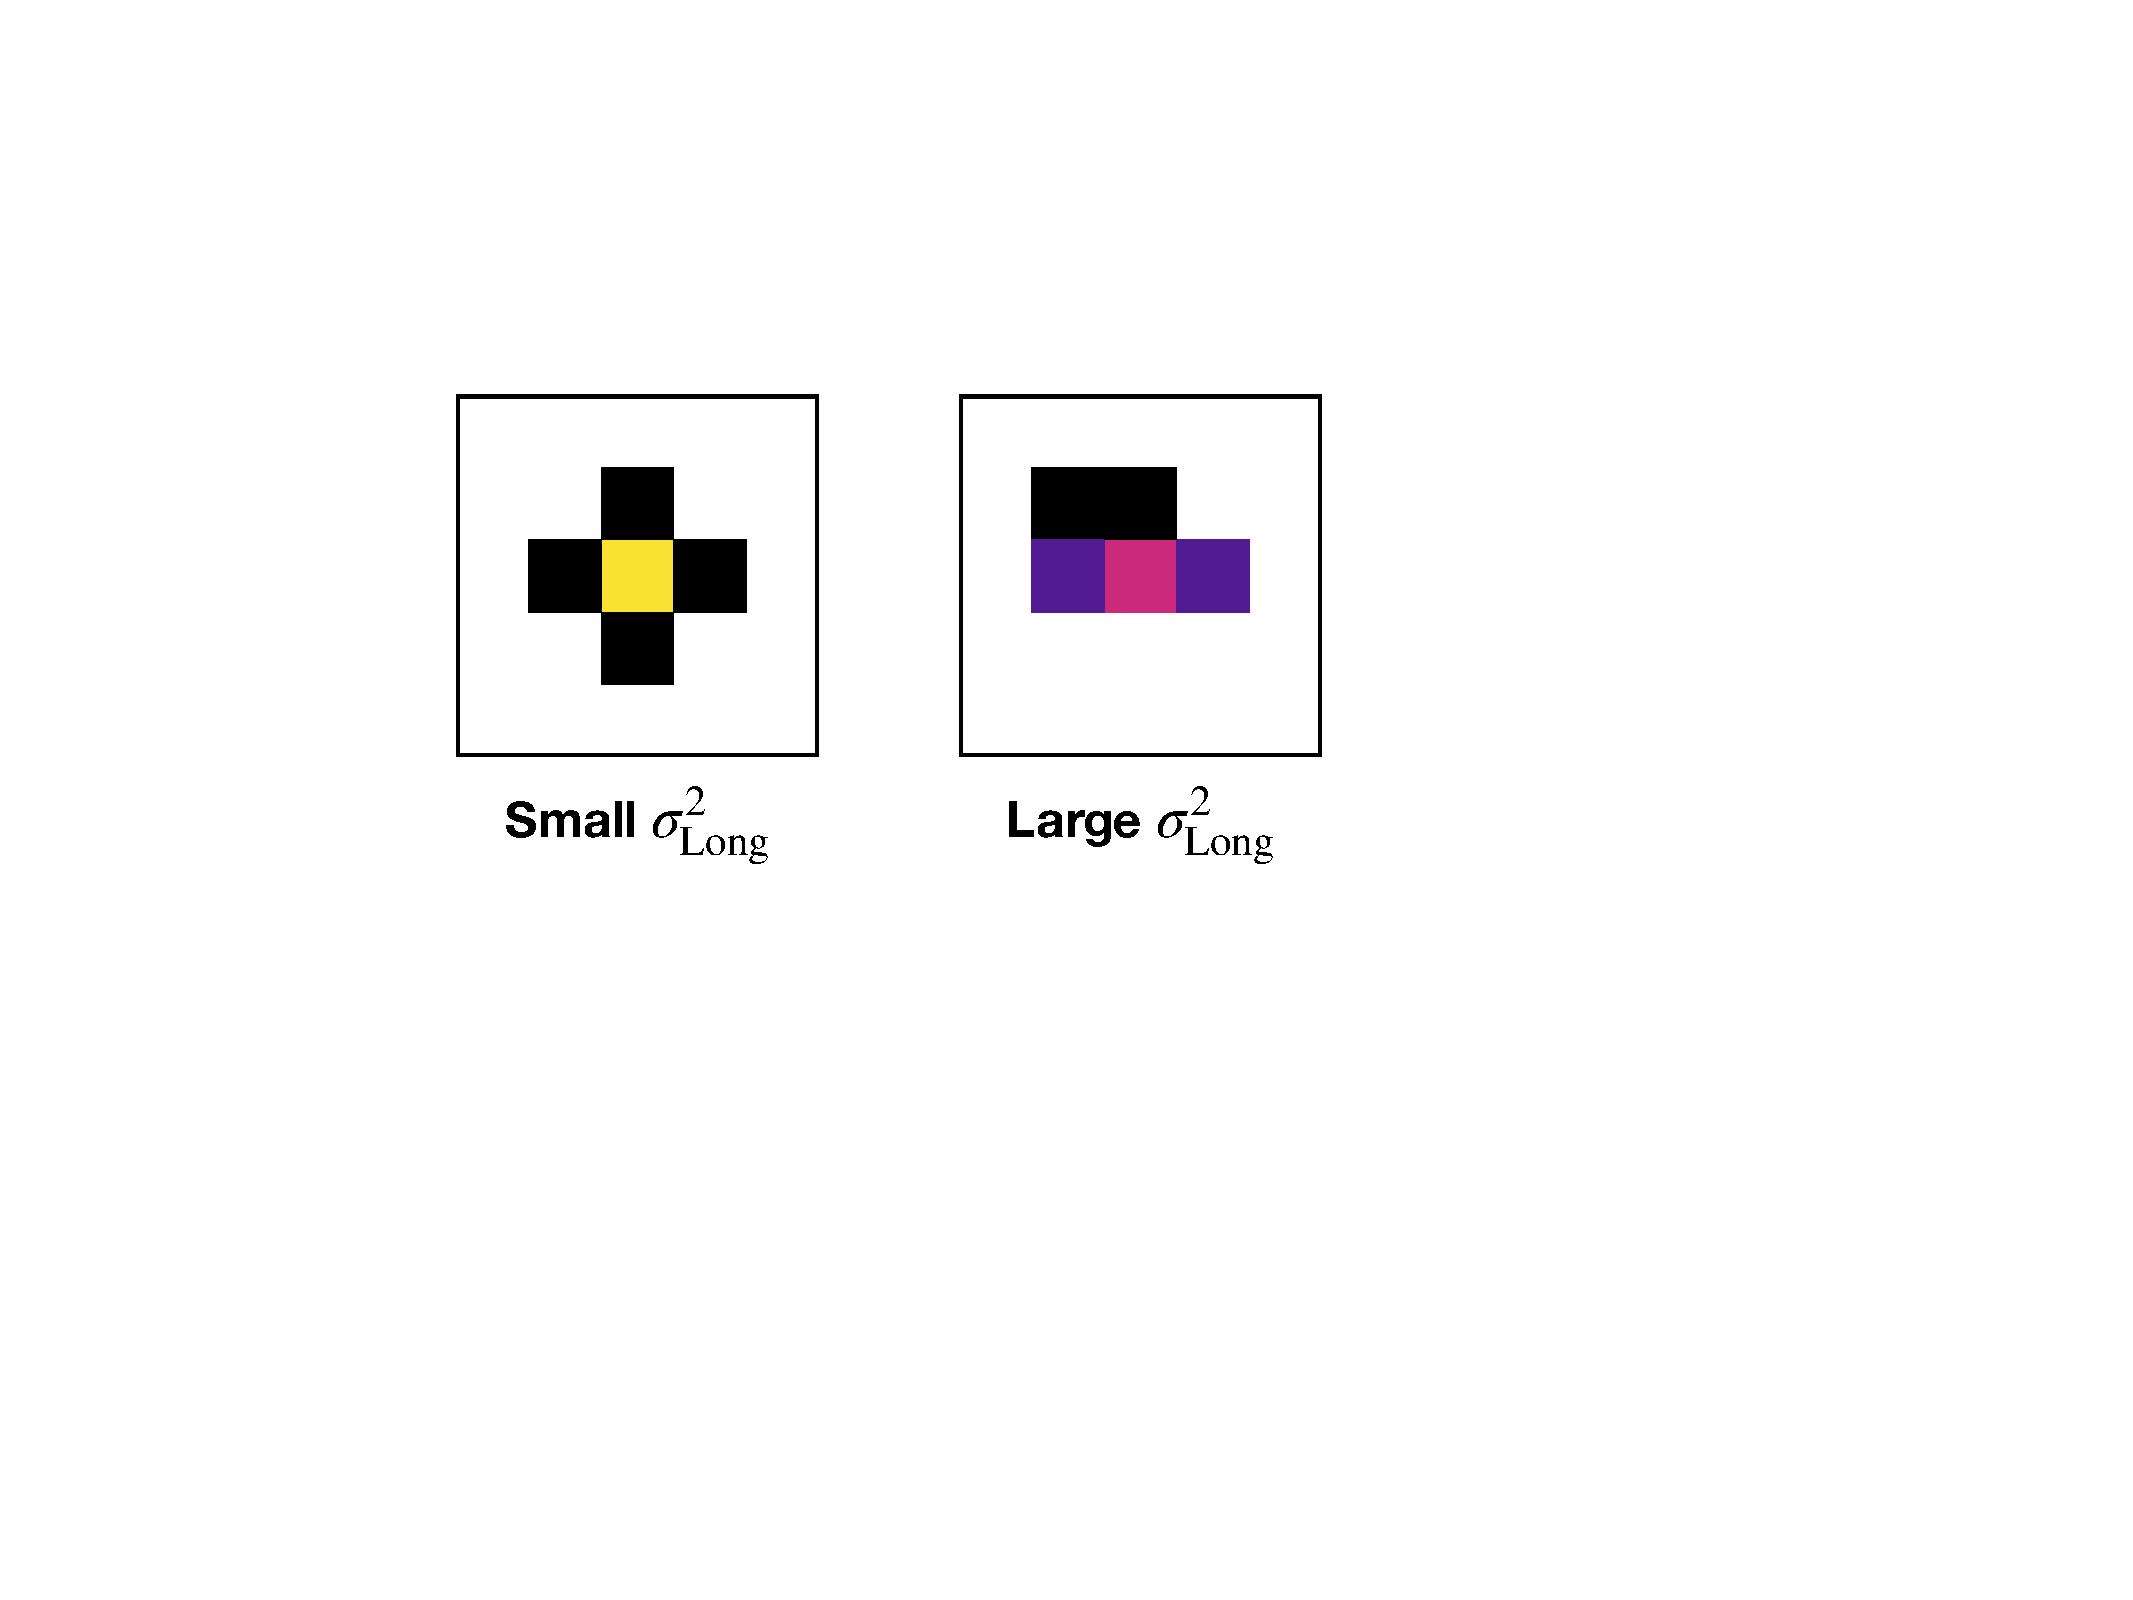
\includegraphics[width=0.5\textwidth]{Data_Analysis/sigma_long_shapes.pdf}
  \caption{Cartoon of a narrow EM shower profile with a small \lambdasquare (left), and an elongated shower profile with a larger \lambdasquare.}
  \label{fig:sigma_long_shapes}
\end{figure}

The shower shape profile is an important tool to help discriminate between clusters belonging to single photons, for which the $\lambdasquare$ distribution is narrow and symmetric, and merged photons from neutral-meson decays, for which the distribution is dominated by a long tail towards higher values. This analysis uses a cutoff of $\lambdasquare < 0.3$ to identify single photon candidates, which will be discussed in Sec.~\ref{sec:purity}.

\subsection{Photon Isolation Requirement}
\label{sec:isolation}
At leading order in pQCD, prompt photons are produced in 2$\to$2 processes surrounded by very little hadronic activity, in contrast to fragmentation photons and high \pt \pizero's found within a jet. Beyond leading order, the direct and fragmentation components cannot be factorized. As a result, the sum of their cross sections becomes the physical observable.\\

Despite this, the contribution from fragmentation photons can be suppressed by enforcing an isolation criteria, where the energy surrounding a photon must be less than a certain threshold. 
Theoretical calculations can also be simplified through the use of an isolation requirement. \cite{PhysRevD.82.014015}. This also has the benefit of suppressing the background from decays of neutral mesons often found within jets.

The simplest definition of isolation is defined as the scalar sum of the transverse momentum of charged particles within an angular radius, $R =\sqrt{(\Delta\varphi)^{2} +(\Delta\eta)^{2}  }$, around the cluster direction. This measurement uses $R = 0.4$, which is a common value used in various jet measurements.

\begin{equation}
\pt^\mathrm{iso,raw} = \sum_{\mathrm{track}~\in\Delta R<0.4} p_{\mathrm{T}}^{\mathrm{track}}	
\end{equation}

This does not, however, take into account the energy arising from the underlying event, described in the following section.
%Define underlying event


\subsection{Underlying Event Estimation for Photon Isolation}
\label{sec:ue_isolation}

The underlying event (UE) is defined as the sum of all processes that make up the final hadronic state in a collision, excluding the leading order hard scattering.When the two neuclei, lorentz contracted into discs tiny fraction of a femtometer thick, overlap or collide, a small fraction of the incident partons suffer hard perturbative interactions as the discs overlap initially. Most of the incident partons, however, lose some energy but are not deflected by any large angle. Most of these interactions are soft and involve little transverse momentum transfer. In the language of fields and particles, as the two discs of strongly interacting transverse color fields and associated color charges collide, some color charge exchange occurs between the discs, and longitudinal color fields are produced, which fill the space between the two receding discs, reducing the energy in the discs themselves, and then gradually decay into $q\bar{q}$ pairs and gluons. These processes can be labelled as multi-parton interactions, as well as both initial and final state radiation, but the term underlying event also includes measured beam fragments. Essentially, the underlying event is made up of all the particles not directly associated with the initial hard scattering of the collision.
% Sources of underlying event can include beam fragments, 

Here we describe the method used to estimate the underlying event for the purposes of correcting the isolation requirement (not to be confused with the later section \ref{sec:ue_subtraction}, where the contribution from the underlying event to the azimuthal correlation measurement is described).

We use the jet area/median method\footnote{From the \textsc{FastJet} software packace::VoronoiAreaSpec \url{http://www.fastjet.fr/repo/doxygen-2.4.5/classfastjet_1_1VoronoiAreaSpec.html} } which estimates the underlying event energy density,~$\rho$, from the median of the distribution of the transverse momentum densities of the jets in the event ~\cite{Cacciari:2009dp}. Jets are reconstructed by running the $k_\mathrm{T}$ reconstruction algorithm over all charged particles in the event, using a resolution parameter of R = 0.3. The \kt algorithm is used here in place of the more standard anti-\kt as it groups particles with the lowest momentum first to construct the jet. This makes the \kt algorithm more sensitive to the softer objects in the event, and therefore more suitable for studying the underlying event.The transverse momentum density of each jet is simply the momentum of the jet divided by its area, determined by the sum of the voronoi cells of each particle within the jet\footnote{The voronoi cell is the region for each "seed", or particle, that  consists of all points in the same  plane that are closer to that seed than to any other.}. 
 This median calculation is described in Equation \ref{eq:ue_density}:
\begin{equation}
\label{eq:ue_density}
  \rho = \mathrm{med} \left\{ \frac{\sum_{i\in J'_k}
    p_{T,i}}{\sum_{i\in J'_k} A_i} \right\}
\end{equation}
where $p_{T,i}$ is the transverse momentum, and $A_i$ the Voronoi area of the particle $i$ within the jet, $J'_k$, reconstructed for UE estimation purpose.  The median is determined from all jets in the event with the important exception of the two leading (highest moment) jets in the event, as those are most often associated with the hard scattering of the collision. This therefore assumes that most of the charged particles in the event is made up of soft particles, and that the charged particles originating from the hard scattering of the collisions are reasonably contained within the leading jets of the event ~\cite{Cacciari:2009dp}.\\

\begin{figure}
\label{fig:Rho}
	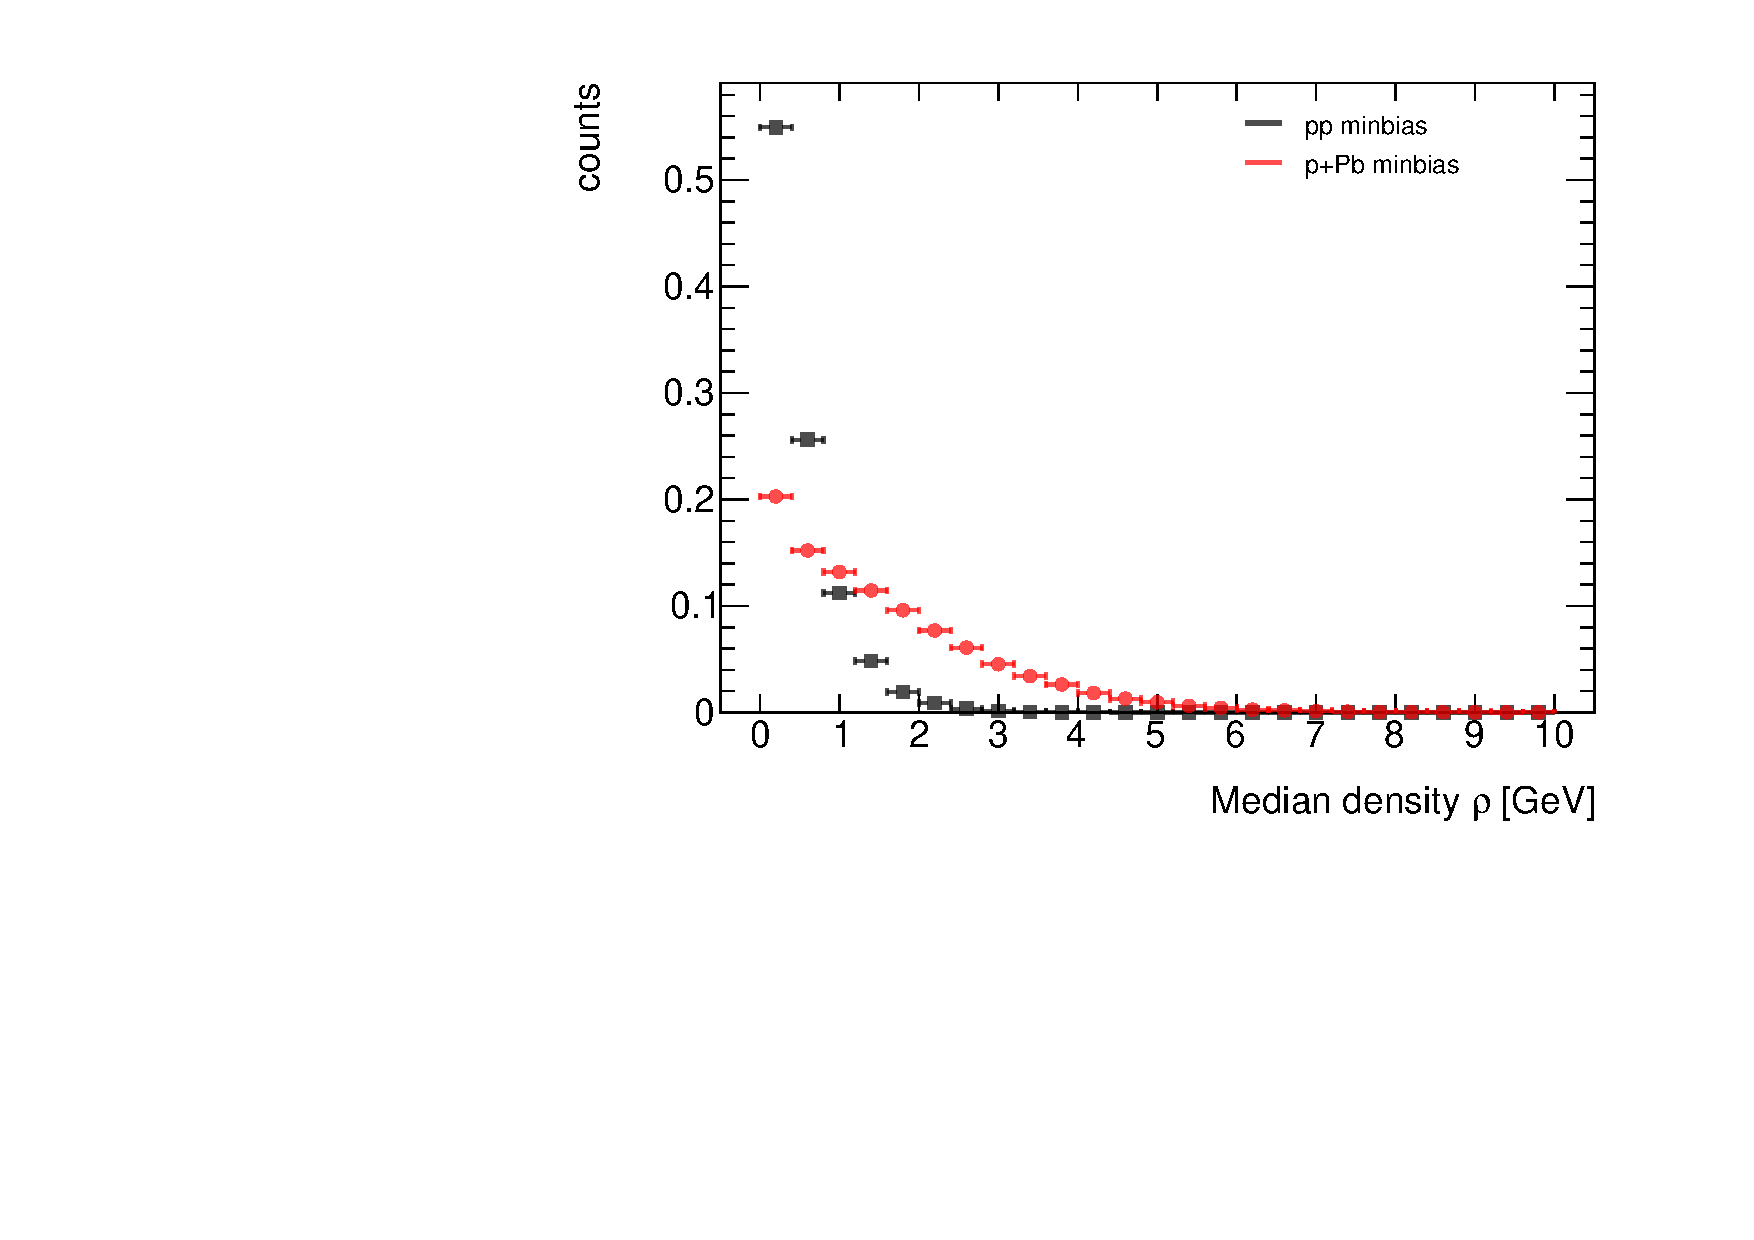
\includegraphics[width=0.5\textwidth]{Data_Analysis/Isolation/Rho_MinBias}
	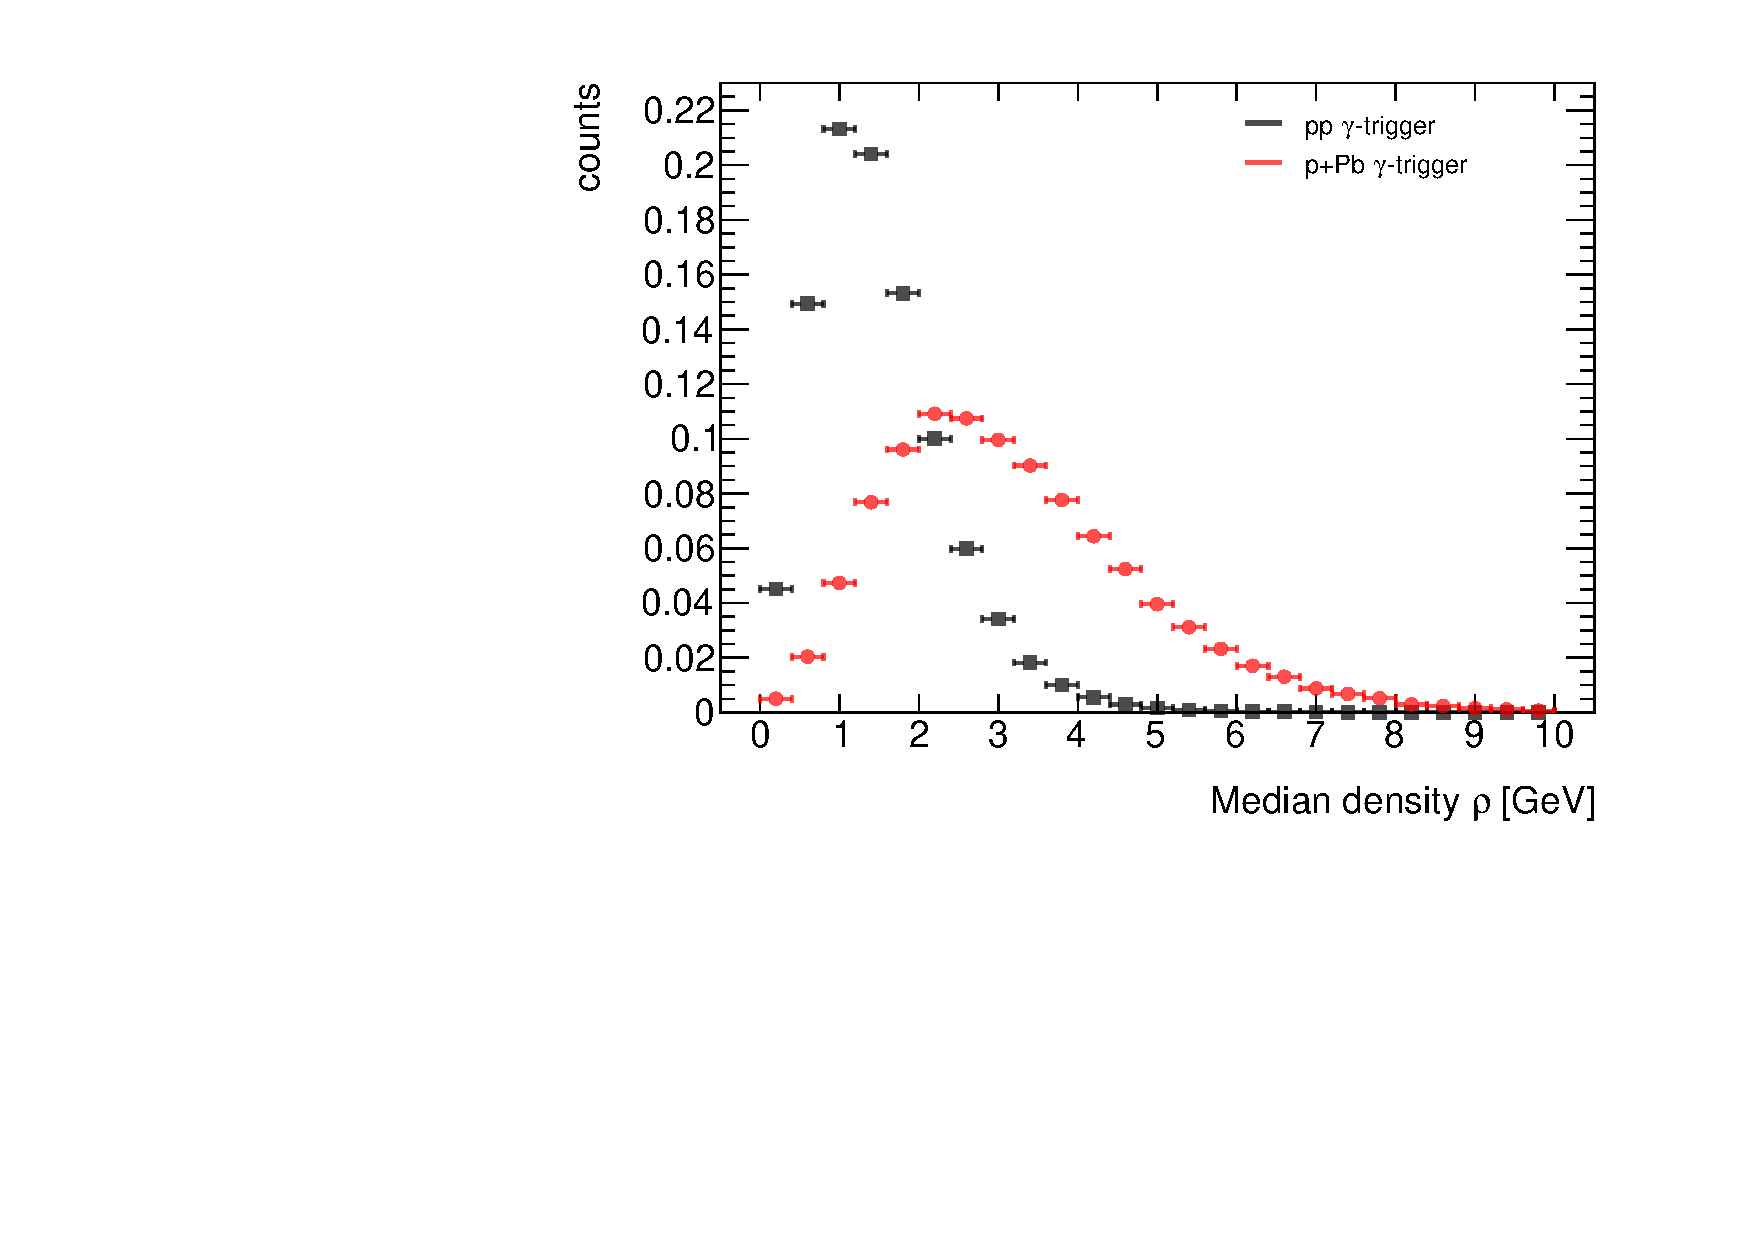
\includegraphics[width=0.5\textwidth]{Data_Analysis/Isolation/Rho_GammaTrigger}
	\caption{Distribution of the median charged-particle transverse momentum density, $\rho$, in pp and \pPb~data, for a minimum-bias selection (left panel) and in photon-triggered events (right panel).}
\end{figure}

The charged-particle density, $\rho$, is calculated for each event. Figure \ref{fig:Rho} shows the distribution of $\rho$ for minimum bias and gamma-triggered events in pp and \pPb. Average values are 3.2 \GeVc~in photon- triggered events in \pPb~and 1.6 \GeVc~in pp collisions, demonstrating the a larger underlying event activity in \pPb compared to pp.


The mean and standard deviation for each distribution is shown in Table~\ref{tab:rhoestimates}. The difference in UE-density in \pPb~is expected due to the increased number of nucleon-nucleon collisions. The UE-densities shown here are still about a factor of 50 lower than in central Pb-Pb collisions.
\begin{table}[h]
   \centering
   \caption{Median transverse momentum density mean and standard deviation in minimum-bias and and photon-triggered events in pp and \pPb~data, calculated with negligible statistical uncertainties.}
   \label{tab:rhoestimates}
   \begin{tabular*}{1.0\columnwidth}{@{\extracolsep{\fill}}lcc|cc@{}}
    \hline
     &  pp minbias & pp $\gamma-$trigger & \pPb~ minbias & \pPb~$\gamma$-trigger  \\
       \hline
       $\langle\rho\rangle$   & 0.49 \GeVc & 1.51 \GeVc & 1.56 \GeVc & 3.19 \GeVc \\ 
       $\sigma_{\rho}$       &  0.47 \GeVc &  0.85 \GeVc  & 1.32 \GeVc & 1.60 \GeVc \\ 
            \hline        
   \end{tabular*}
\end{table}

%TODO: Write about lack of neutrals in isolation
%isolation variable does not include neutral particles. This enables us to use the full acceptance of the EMCal and reduces biases arising from correlation with the opening angle of $\pi^{0}$ decays. However, it does result in a slightly lower purity of the isolated single photon signal. 

\subsection{UE Correction to Isolation Variable}
\label{sec:ue_correction_isolation}
For each cluster in the event, the underlying event is subtracted using the measured charged-particle density $\rho$ that is calculated event-by-event as described in Section~\ref{sec:ue_isolation}:

%For the determination of the isolation criterium,~$\pt^\mathrm{iso}$, the background due to the underlying event is estimated with the Voronoi method from the \textsc{FastJet} jet area/median package~\cite{Cacciari:2009dp} on an event-by-event basis and subtracted according to:

The result is an average subtraction for the isolation cone of {$R=0.4$} is about {$1.6$ \GeVc} and {$0.8$ \GeVc} for \pPb~and pp collisions, with a standard deviation of {0.9 \GeVc} and {0.4 \GeVc}, respectively.  

%A requirement of $\pt^\mathrm{iso}<1.5$ \GeVc is used, which results in a signal efficiency of about 90$\%$ that does not significantly depend on the photon $\pt$. 
 
For photons near the edge of the detector, the isolation energy requirement is scaled to account for any missing area in the isolation cone\footnote{The final isolated photon-hadron correlations are normalized to the number of reconstructed photons. As a result, the $\gammaiso$ efficiency was not studied in detail.}. A check on on this scaling procedure was also done in Section \ref{sec:iso_acceptance_check}. 
\begin{equation}
p_T^\mathrm{iso} = p_T^\mathrm{iso,raw} - \rho\times\pi(0.4)^{2}.
\end{equation}

Figure~\ref{fig:iso_ue} shows the isolation distribution before and after underlying event subtraction for \pPb~and pp collisions. The distributions have a positive tail that decreases exponentially. This is likely due to the sensitivity of the isolation variable on multi-jet production cross section. The difference between the \pPb~and pp distribution at low $\ptiso$ values can be attributed to the effect of enhanced soft-particle production in \pPb~collisions, i.e. a larger underlying event due to the presence of the pPb nucleus. The underlying event subtraction modifies the isolation distribution only slightly at high \pt. At low and negetaive \pt, however, the distributions show a negative tail after subtraction, which arises from an over-subtraction of the underlying event. This occurs due to region-to-region fluctuations in the underlying event, where a cluster contains an energy density that is smaller than the median calculated according to Section \ref{sec:ue_isolation}. In both cases, this tail falls by more than three orders of magnitude by $\ptiso=-3$ \GeVc, indicating that over-subtraction is a small effect.   

\begin{figure}[h]
\center
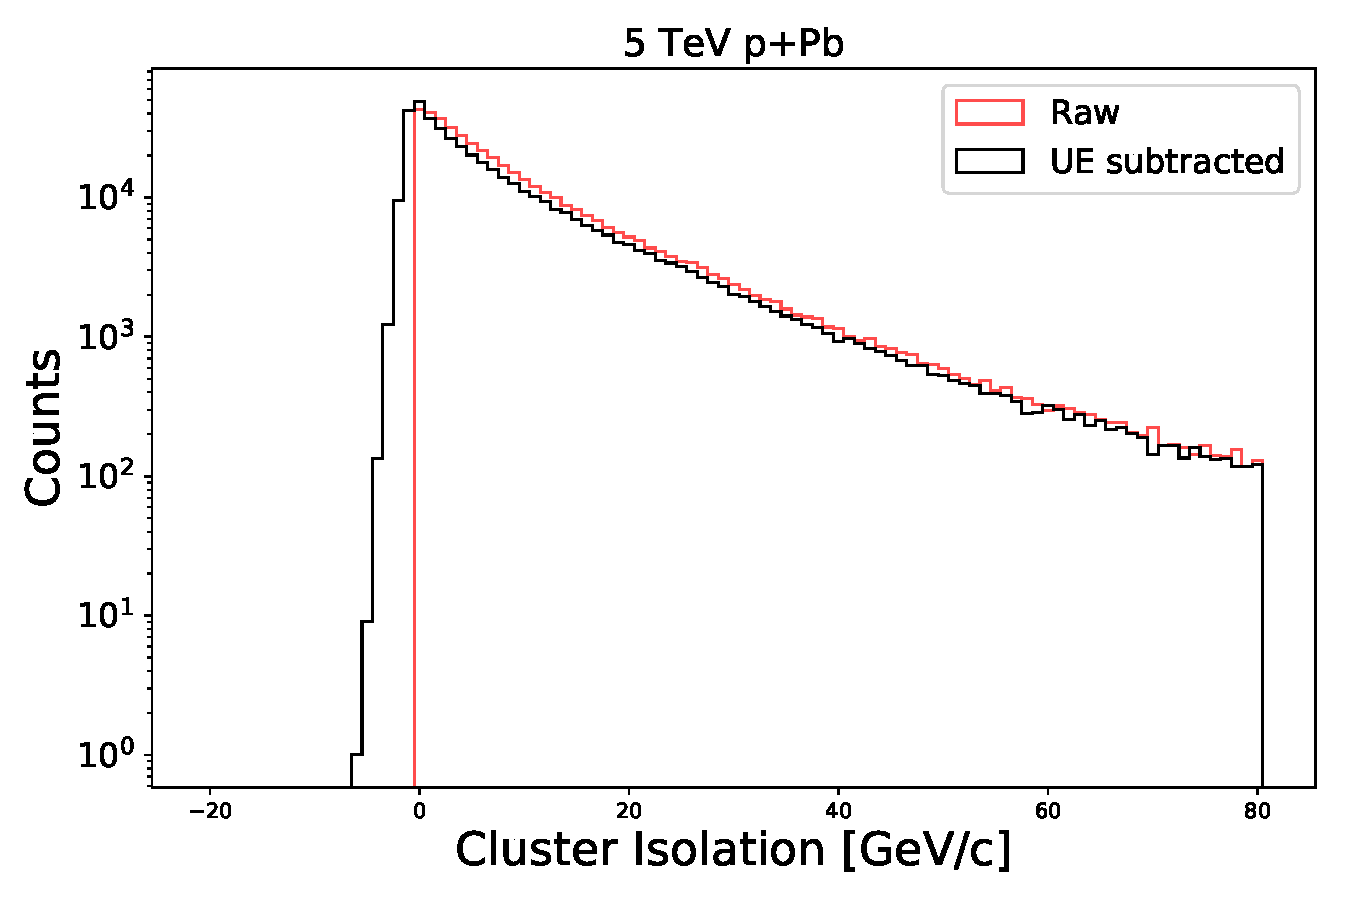
\includegraphics[width=0.49\textwidth]{Data_Analysis/Isolation/IsolationWithUESubtraction_Skimmed_13def_root}
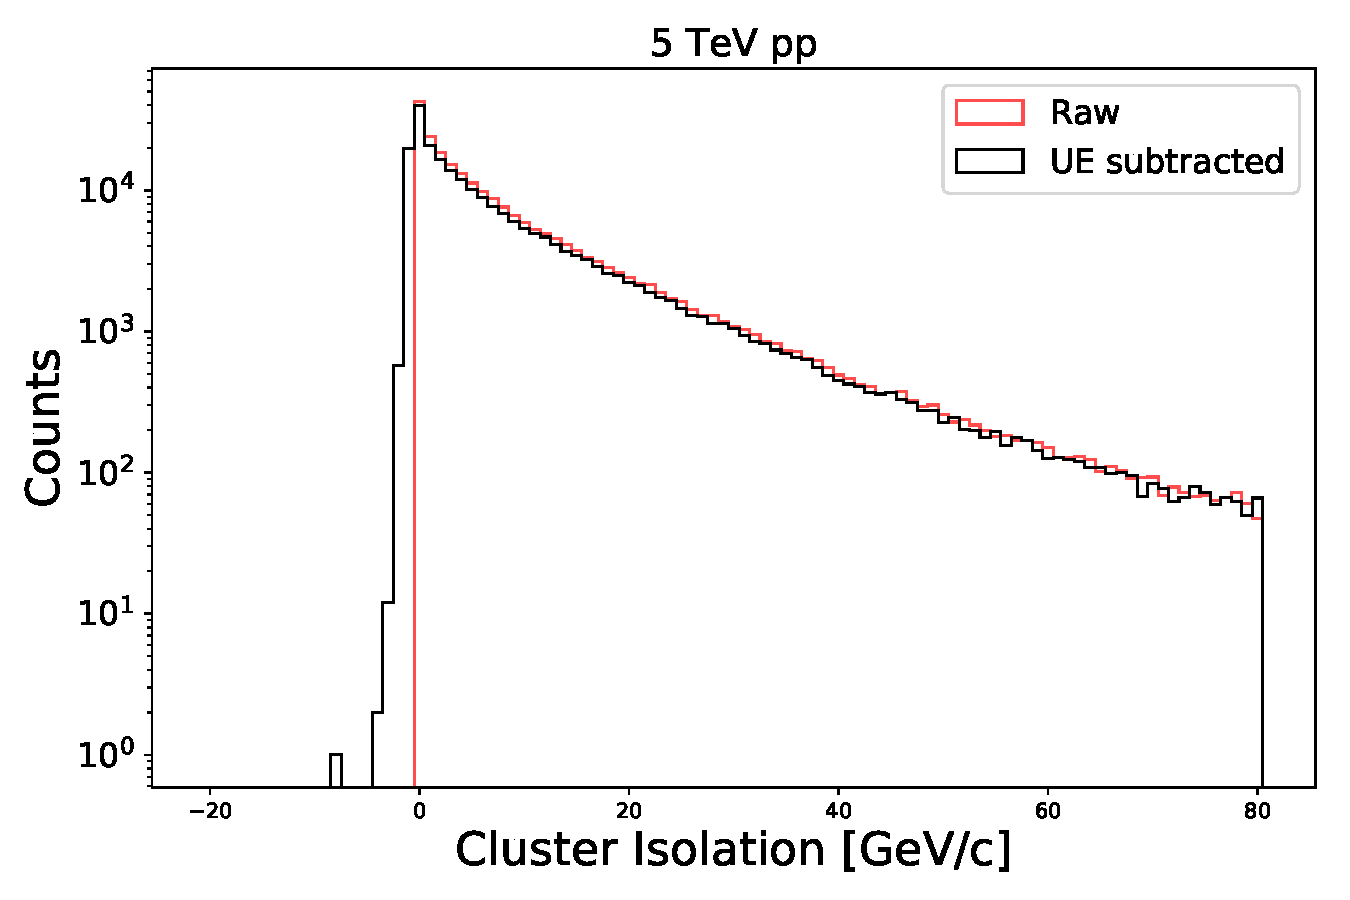
\includegraphics[width=0.49\textwidth]{Data_Analysis/Isolation/IsolationWithUESubtraction_Skimmed_17q_root}
\caption{Cluster isolation before and after underlying event subtraction in \pPb~(left panel) and pp (right panel) collisions.}
\label{fig:iso_ue}
\end{figure}

%TODO Fix Table Reference
The left panel of Figure~\ref{MC_Isolation} shows the distribution of cluster isolation after UE subtraction for photon-jet and dijet simulations of \pPb~data (see Table~\ref{tab:MCsamples}). The distributions exhibit different behavior: whereas the dijet simulation shows a prominent exponential tail at large $\ptiso$ values, the photon-jet simulation shows a more Gaussian-like shape that is mostly symmetric with the exception of a very small fraction of events that have large $\ptiso$ values. In both cases, however, the negative tail falls rather sharply, as it arises from region-to-region fluctuations of the UE that are independent of the hard-process involved. 

\begin{figure}[h]
\center
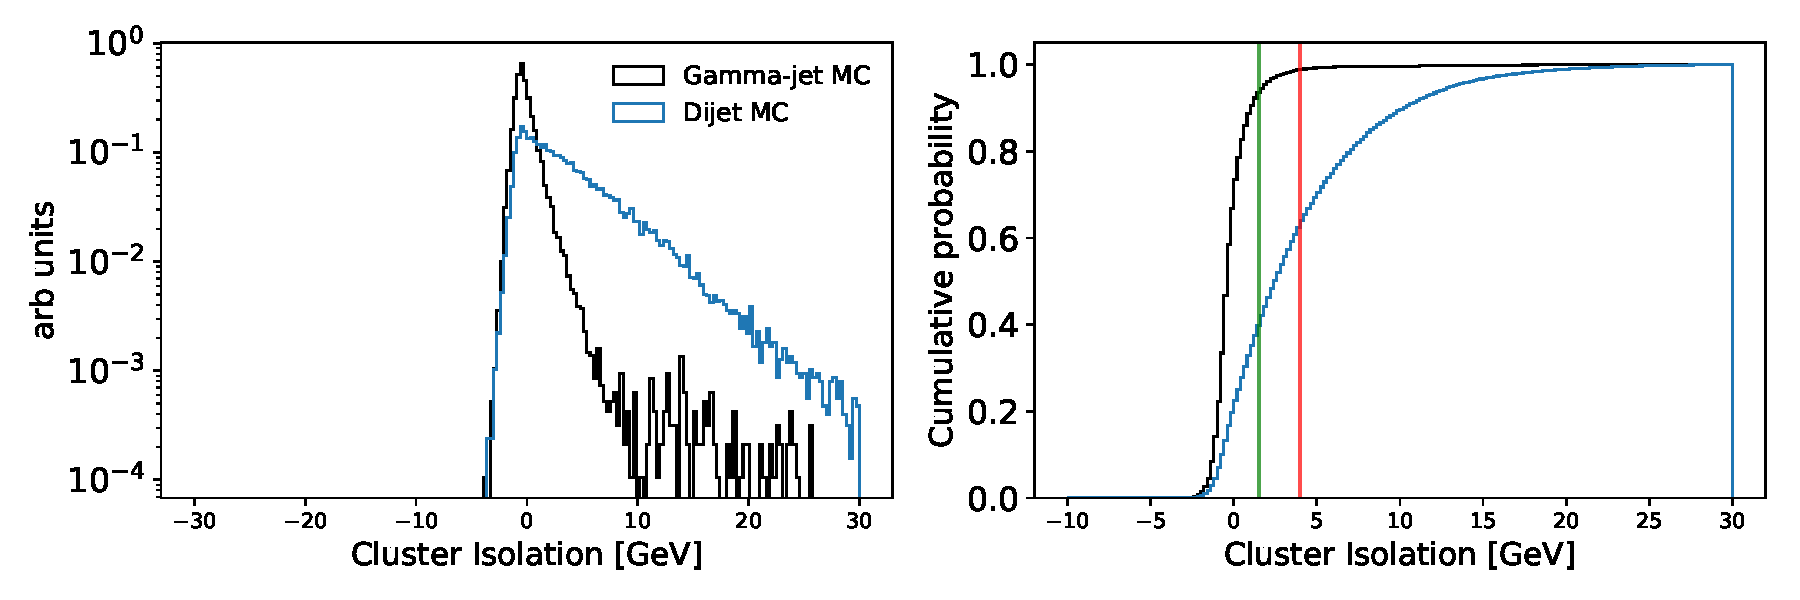
\includegraphics[width=1.0\textwidth]{Data_Analysis/Isolation/IsolationMCsignal_Skimmed_17g6a1_pthat1_4L_root}
\caption{Isolation distribution of clusters that pass our selection in \pPb~photon-jet and dijet simulations, and corresponding cumulative distribution. Two vertical lines at $\ptiso=$ 1.5 \GeVc~(green) and $\ptiso=$ 5.0 \GeVc~are shown in the right panel for reference.}
\label{MC_Isolation}
\end{figure}

%For the purposes of template fitting, we also need to define a sideband that is dominated by background. For this we note that only about 1$\%$ of prompt photons of the photon-jet simulation have {$\iso>$ 5 \GeVc}. Given that the cross-section for prompt photons is about two orders of magnitude smaller than the background, this region is overwhelmingly dominated by background.   

The cumulative distributions (Figure~\ref{MC_Isolation}, right panel) show that a {$\ptiso<$ 1.5 \GeVc} selection keeps about 90$\%$ of the signal and rejects about 60$\%$ of the background. This relatively loose photon isolation criteria is used in order to reduce the dependence of the results on the details of the simulation of the detector noise, tracking resolution, and the underlying event. 


\subsection{Remaining Background after Photon Selection}

This isolation cut of {$\ptiso<$ 1.5 \GeVc} is used in conjunction with the shower-shape cut  of $0<\lambdasquare<0.3$ to complete the isolated-photon selection or ``$\gammaiso$ selection''. The population of clusters that pass this selection are labelled``$\gammaiso$-candidates'' (rather than simply ''prompt photons'') because there is still a significant fraction of remaining background. Some other sources of background not yet mentioned arise from charged-to-neutral fluctuations of jet fragmentation that leads to low observable $\ptiso$ (that considers only charged-particles). However, the main background present in the $\gammaiso$ selection arise from multi-jet events where one jet typically contains a $\pi^{0}$ or $\eta$ which carries most of the jet energy, and is therefore surrounded by relatively less energy within the jet. The pair is also frequently misidentified as a single photon because it decays into a pair of photons that are collinear with respect to the EMCal cell granularity. The first indication of this is shown in Figure \ref{MC_Isolation}, where approximately 40\% of the dijet cross section (expressed as a cumulative probability as a function of cluster isolation, shown in blue) is within $\ptiso < 1.5 \GeVc$.\\ Distributions of background and signal as function of \lambdasquare are shown later in \ref{sec:purity}

Figure \ref{fig:cross_section_camparison} expands on this. The left panel shows the isolated photon differential cross section as a function of \ptgamma in proton-proton collisions at \sqrts = 5.02 TeV measured by the ALICE detector. The right panel of Figure shows the differential cross section of charged jets as a function of $\pt^\mathrm{jet}$. The cross section for an isolated photon at \pt = 20 \GeVc~is roughly 2nb $\GeVc^{-1}$. In contrast, the cross section for charged jets at \pt = 20 \GeVc~is roughly 2$\times10^{-3}$mb $\GeVc^{-1}$, approximately three orders of magnitude larger. 

\begin{figure}
\centering
	\label{fig:cross_section_camparison}
\raisebox{0.9cm}{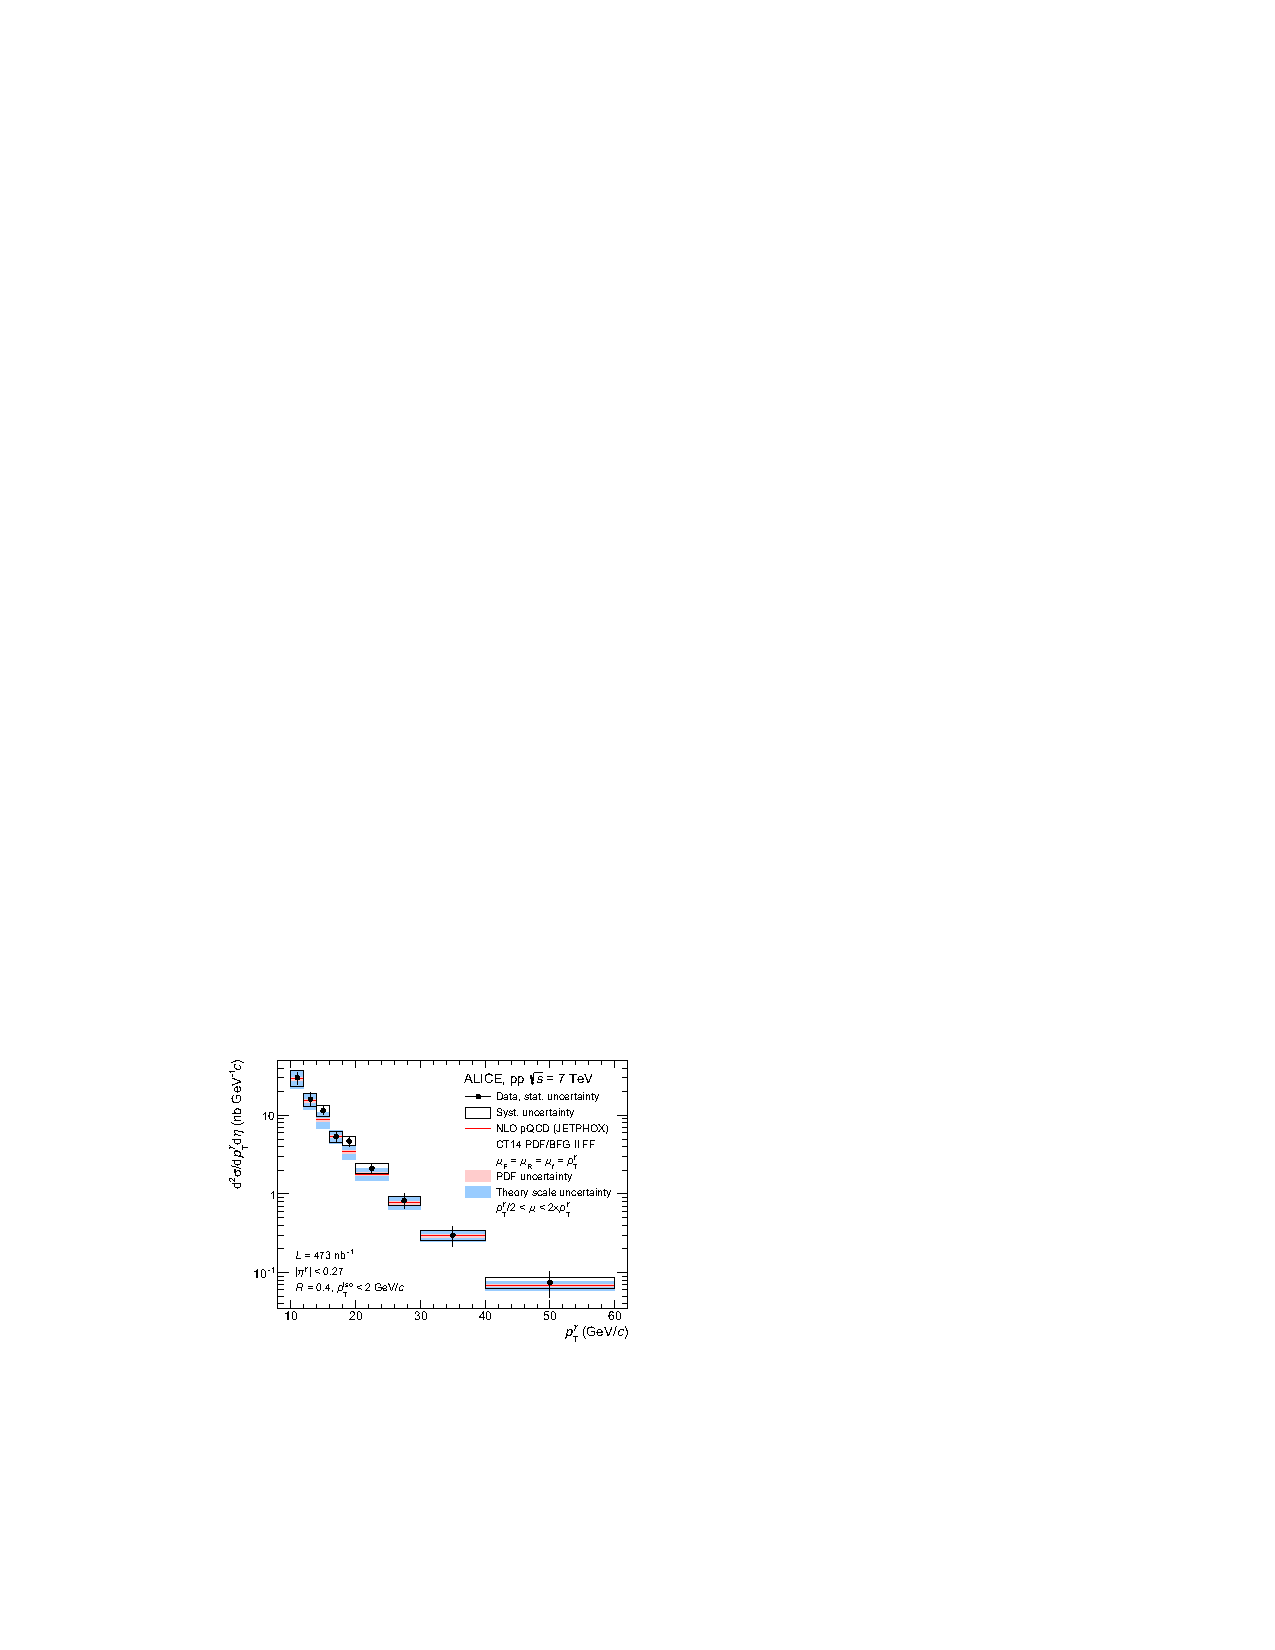
\includegraphics{Data_Analysis/Isolation/isolated_photon_cross_section}}
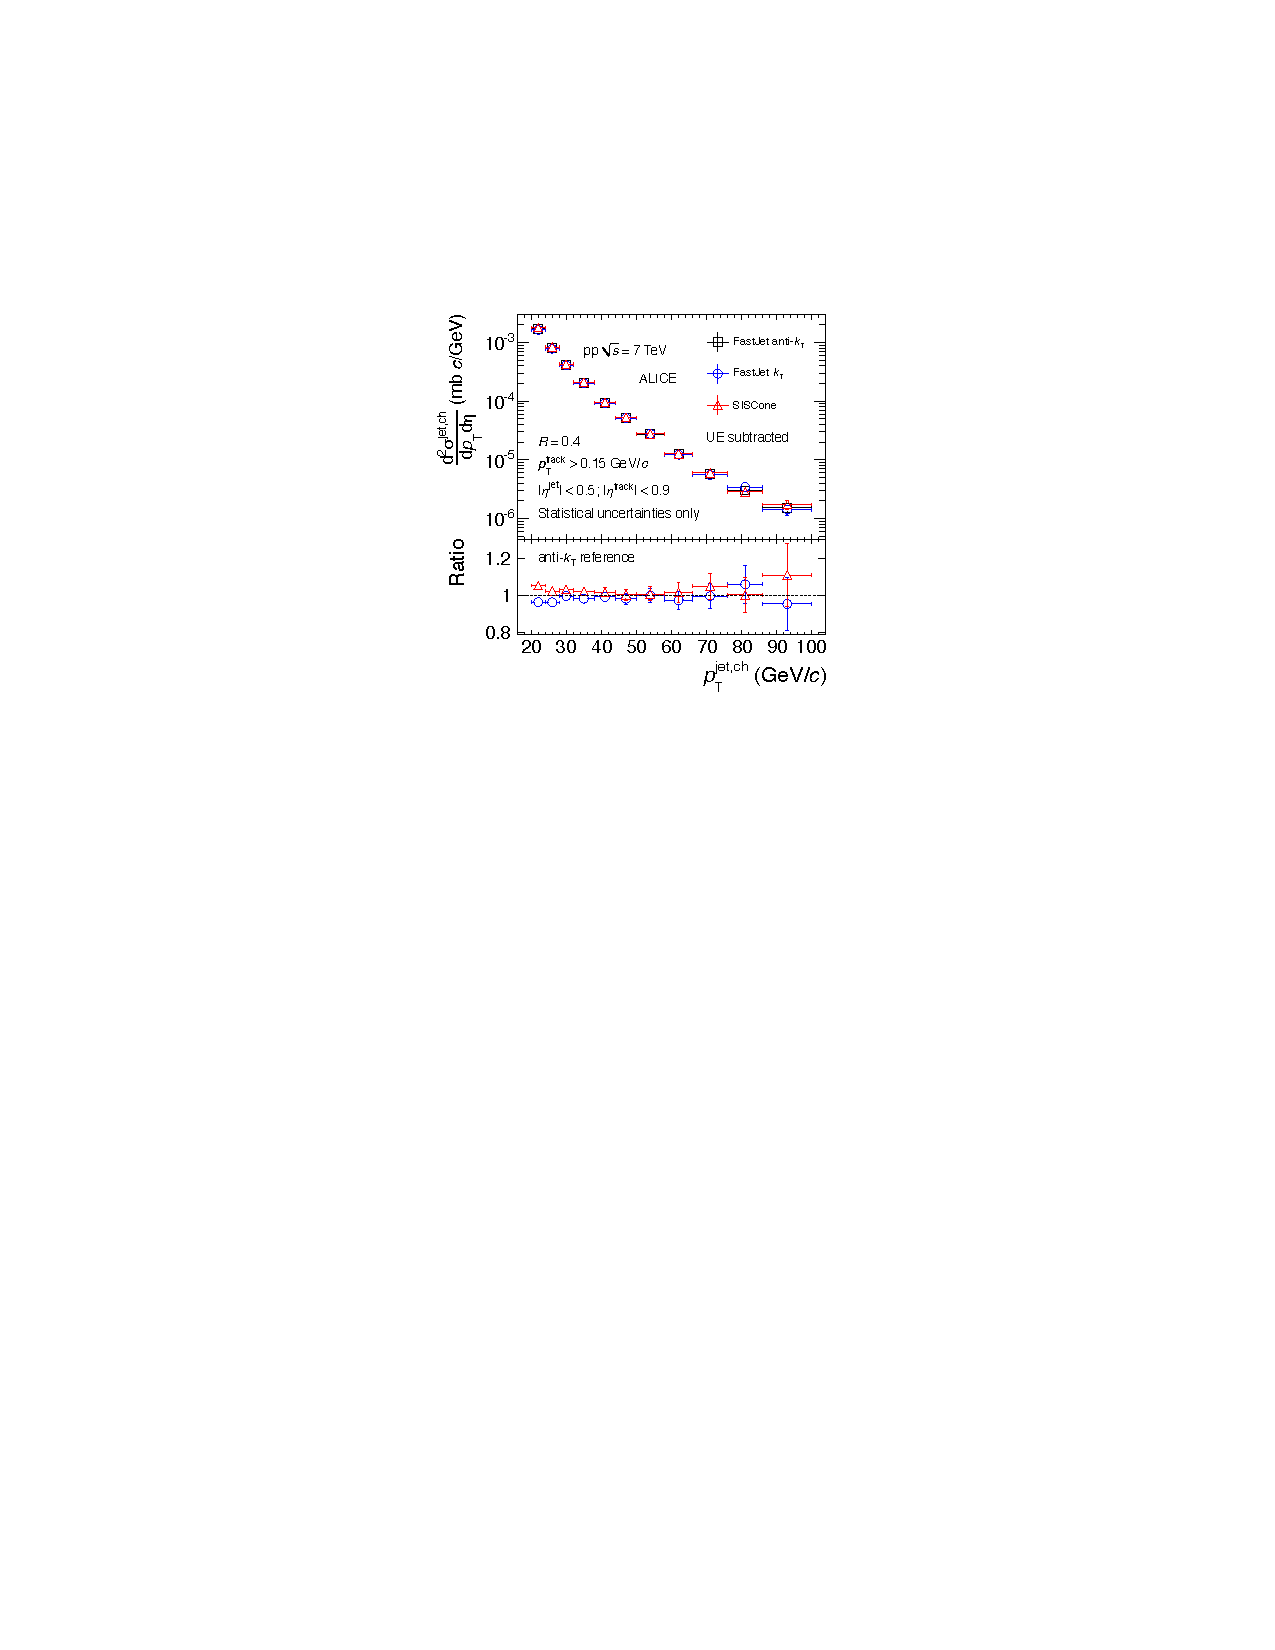
\includegraphics{Data_Analysis/Isolation/charged_jet_cross_section}
\end{figure}

 

Of course, jets containing a neutral meson with a large fraction of its total momentum make up only a fraction of the total jet cross section, and recoil partons produced from the same hard scattering as prompt photons will contribute to the total charged jet cross section. But the stark difference between the isolated photon and charged jet cross sections speaks to the rarity of isolated photons in these collisions and the abundance of background and illustrates the need to measure the purity of our $\gammaiso$-candidate selection.%, which is described in Section~\ref{sec:purity}. 

%r



%A \pizero with sufficiently high \pt, approximately 6~\GeVc, a \pizero will decay into two photons with such a small opening angle, that their electromagnetic showers from the two photons in the ALICE EMCal significantly overlap. %significantly overlapping elecromagnetic showers in the calorimeter
%For this reason, the two showers from the two photons will appear in the ALICE EMCal as a single cluster.

%Thus, in order to select against this measurement's largest source of background, we require that clusters have a more symmetric shape in the EMCal.
\section{Purity}
\label{sec:purity}
The isolation and shower shape selections remove the bulk of the neutral meson decay background, but a substantial fraction of the \gammaiso candidates are still background photons. It is therefore necessary to quantify the ratio of true signal photons in our candidate sample in order properly subtract it. The estimate of the ratio of true signal photons in our \gammaiso sample is called the \textit{purity}. \footnote{For a more rigorous discussion of the Purity calculation, please see Alwina Liu's UC Berkeley Thesis.}

\subsection{The Template Fit Method}
The purity of the isolated photon sample is determined with a two-component template fit, a method used by the CMS collaboration in Ref.~\cite{Sirunyan:2017qhf}. The distribution of the shower shape variable for the isolated cluster sample is fit to a linear combination of a signal distribution and the background distribution. The shape of the signal distribution is determined by a photon-jet simulation (see Table~\ref{tab:MCsamples}) and the shape of the background distribution is determined from data using an anti-isolated sideband~\footnote{The inversion of an isolation cut to estimate QCD background is a standard technique in several measurements at the LHC and previous hadron colliders.} with an additional correction computed from a dijet simulation. This is described in more detail in the following sections.  

\subsection{Signal Template and Background Templates }
The shape of the background distribution of the shower-shape for isolated clusters is estimated with a \textit{sideband} technique: the shower shape distribution of clusters from isolated decay photons is estimated with clusters that are anti-isolated but pass all other selection criteria. This method assumes that the correlation between the isolation variable and shower shape variable can be corrected for; the procedure for doing so is described below. The signal and sideband regions defined using the isolation variable are illustrated in Figure~\ref{SidebandDefinition}. 

\begin{figure}[h]
\center
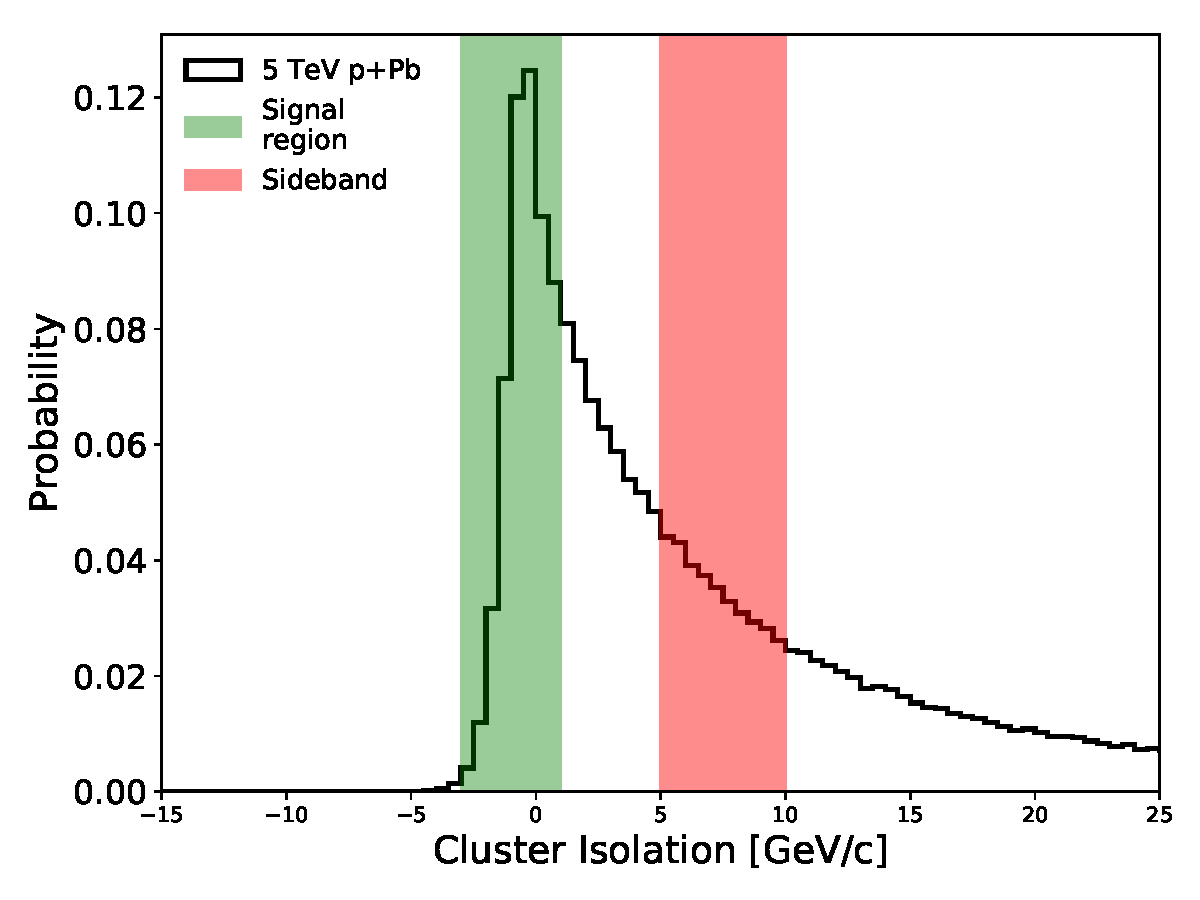
\includegraphics[width=0.49\textwidth]{Data_Analysis/Purity/IsolationSideband_limited_Skimmed_13def_root}
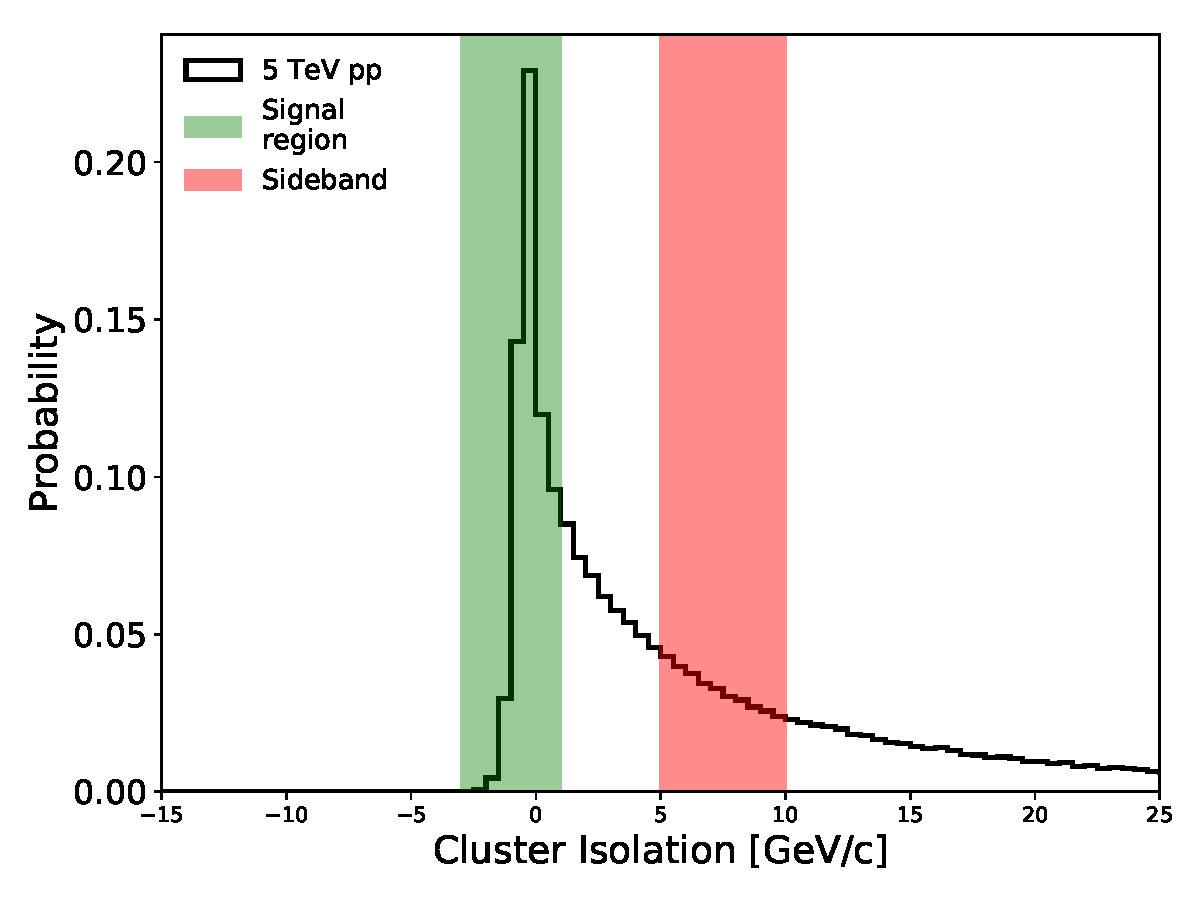
\includegraphics[width=0.49\textwidth]{Data_Analysis/Purity/IsolationSideband_limited_Skimmed_17q_root}
\caption{Isolation variable distribution of clusters with $\pt$ between 12 and 16 \GeVc~in \pPb~data (left panel) and pp data (right panel). The green shaded are represents the signal region ($\iso<$ 1.5 \GeVc); the red represent the sideband ($5<\iso<10$ \GeVc) used to estimate the background template.}
\label{SidebandDefinition}
\end{figure}

For simplicity, the same definitions are used for pp and \pPb~data. The lower bound of the sideband region is defined as {$\iso=5$ \GeVc}; according to photon-jet simulations, less than 1$\%$ of prompt photons are beyond this range. The upper bound is chosen such that the sideband is as narrow as possible, to minimize a possible bias to the shower-shape distribution due to a positive correlation with ISO, while still containing a number of clusters comparable to the signal region. A more rigorous study on the sensitivity of our purity estimate on the choice of sideband region is shown in Section~\ref{sec:bkgtemplate}.

Figure~\ref{TemplateShapes} summarizes the signal and background templates used in the template fit. The distributions are quite different, which is key for the stability of the template fit. The background shape in the $\lambdasquare$ variable shows a peak in the single-shower region but a ``bump'' that reflects a $\pi^{0}$ peak. In both cases, the peaks in the single-shower region that are observed in the background templates come mostly from collinear $\pi^{0}\to\gamma\gamma$ decays.

\begin{figure}
\center
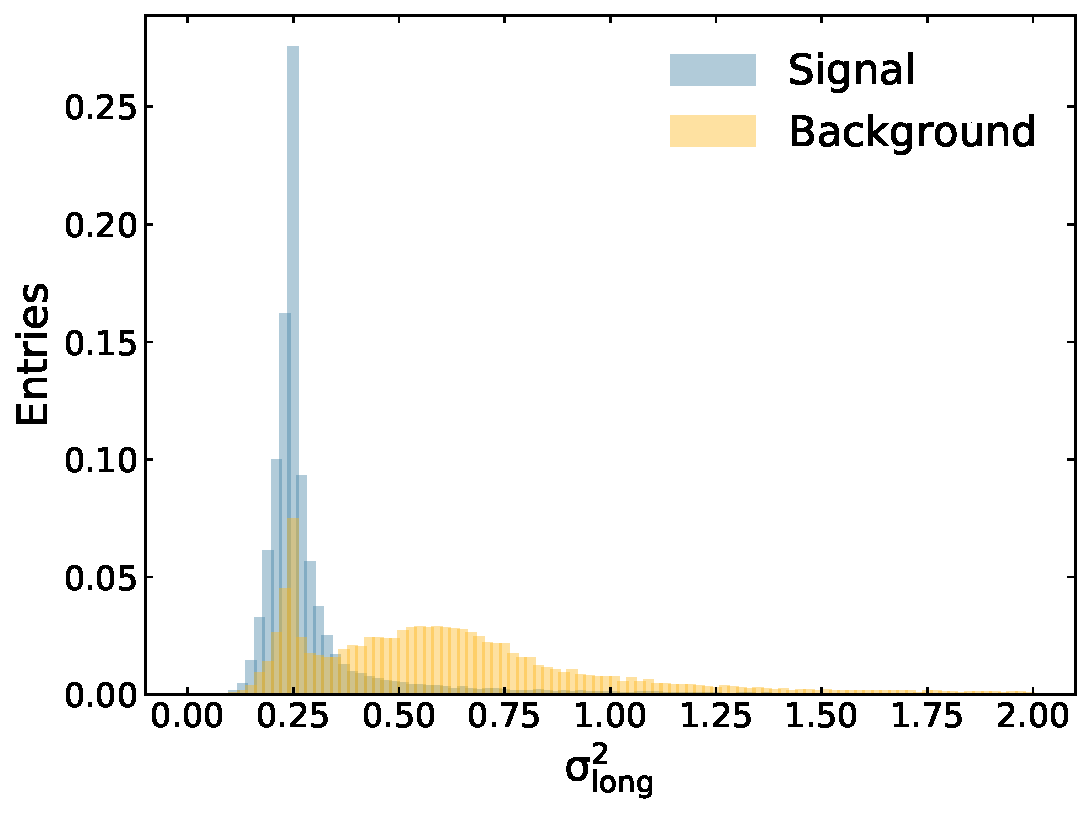
\includegraphics[width=0.5\textheight]{Data_Analysis/Purity/norm-templates-p-Pb-cluster_Lambda-15-20.pdf}
\caption{Normalized signal (blue) and background (yellow) distributions used as input for the template fit. These distributions correspond to clusters with \pt~in the 15--20 \GeVc~range.}
\label{TemplateShapes}
\end{figure}


The background template is corrected for a bias due to correlations between the shower-shape and isolation variables \cite{Khachatryan:2010fm}. 
%bvj In particular, the 
This correlation leads to clusters in the isolation sideband having a somewhat higher hadronic activity than the true isolated background. Consequently, a background template constructed from this sideband region has an increased number of background-like clusters and
%bvj which enhances the background-like region of the shower-shape distribution. This implies that the 
purity values obtained using this
 systematically overestimate the true purity.
A correction for this bias, $R(\lambdasquare)$, is determined using dijet simulated events which also contain the correlation between trigger photon shower-shape and isolation cut.
The ratio of the shower-shape distributions of clusters in the signal (Iso, $\pt^\mathrm{iso} < 1.5$ \GeVc) region and sideband (Anti-iso, $5.0 < \pt^\mathrm{iso} < 10.0$ \GeVc) region is constructed via

%The ratio of the shower-shape distributions of clusters in the signal (Iso) region and sideband (Anti-iso) region is constructed via

\begin{equation}
    R(\lambdasquare)=\frac{\text{Iso}_{\text{MC}}(\lambdasquare)}{\text{Anti-iso}_{\text{MC}}(\lambdasquare).}
    \label{eq:bkgtemplateweights}
\end{equation}
%{\color{red}  I think that a referee and our collaborators will want to know what was chosen for the sideband region. So, I suggest we just stick in the information from the start.}
This ratio of shower shape distributions is applied as a multiplicative correction to the background template:

\begin{equation}
    B^{\text{corr.}}(\lambdasquare)=\text{Anti-iso}_{\text{data}}(\lambdasquare)\times R(\lambdasquare).
    \label{eq:bkgtemplatecorrection}
\end{equation}

This background template correction results in an absolute correction on the purity of 8$\%$--14$\%$ depending on the cluster $\pt$. An example of a fit with and without the correction is shown in Figure~\ref{fig:purcorrectionexample}. The correction greatly improves the fit. 


% The purities as a function of the cluster $\pt$ are shown in Figure~\ref{fig:Purity}. 
% The background template is corrected for the correlation between the shower shape  variable and the isolation energy of the cluster. A dijet simulation is used to construct the ratio of the shower shape distribution for isolated clusters to the shower shape distribution for anti-isolated clusters. This ratio, calculated as a function of the shower shape variable, is then applied as a weight to the anti-isolated clusters in the data, giving a corrected background template that is then used in the template fit. From Equ.~\ref{eq:bkgtemplatecorrection}), it is clear that if the monte-carlo exactly replicates the data, the Weights function will exactly correct the anti-isolated decay photon \lambdasquare distribution back to the isolated decay photon \lambdasquare~distribution, which is the true background.\\ 

% \begin{align}
%     \text{Weights}(\lambdasquare)&=\frac{\text{Iso}_{\text{MC}}(\lambdasquare)}{\text{Anti-iso}_{\text{MC}}(\lambdasquare)} \nonumber \\
%     \text{Bkg}^{\text{corrected}}(\lambdasquare)&=\text{Non-iso}_{\text{data}}(\lambdasquare)\times\text{Weights}(\lambdasquare)
%     \label{eq:bkgtemplatecorrection}
% \end{align}

% The purity computed with the corrected background template is 8--13\% (absolute) lower in compared to the purity computed with the uncorrected background template; 

\begin{figure}
    \centering
    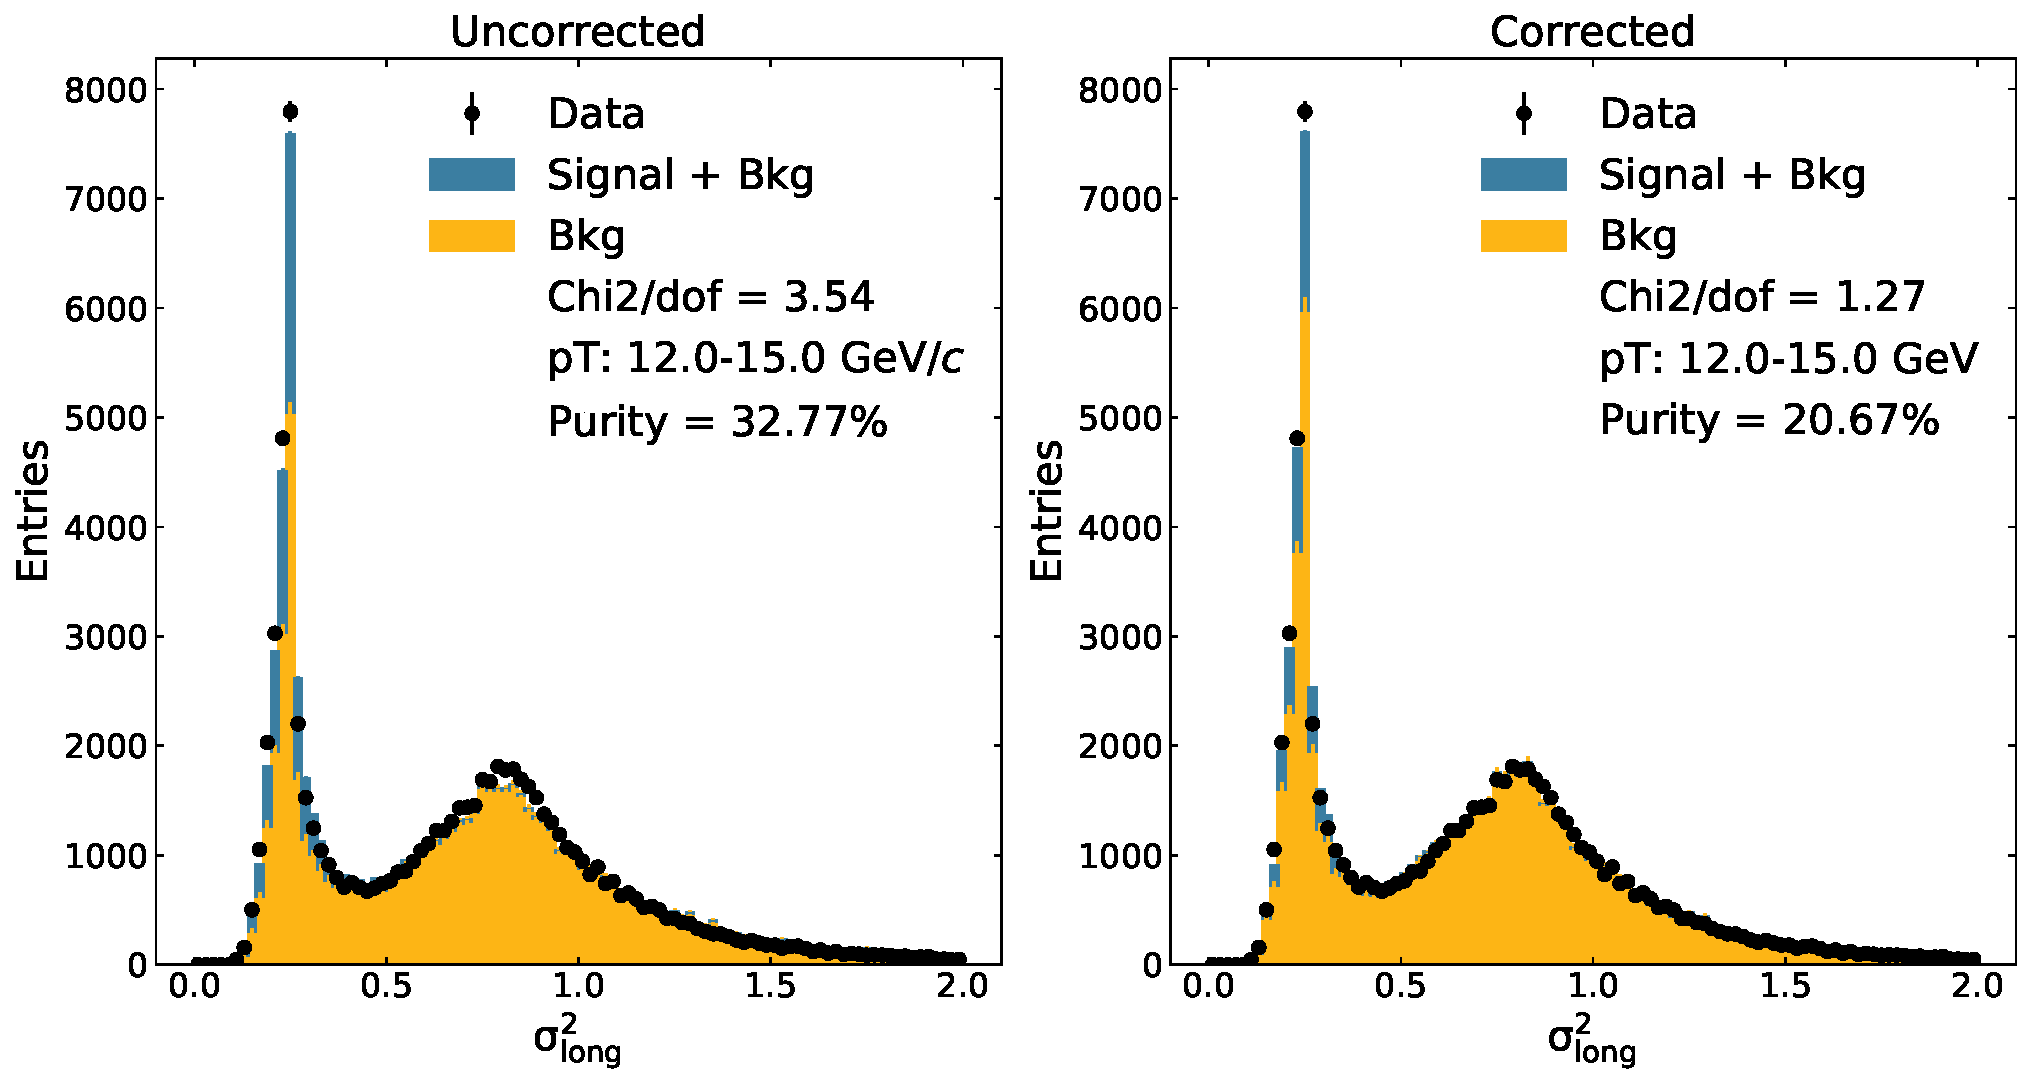
\includegraphics[width=0.5\textheight]{Data_Analysis/Purity/correction-example-p-Pb-cluster_Lambda-12-15.pdf}
    \caption{An example of the template fit with and without the background template correction in \pPb~for clusters with $12 < \pt < 15$ GeV/$c$. The goodness of fit is better after the correction and the purity is significantly lower.}
    \label{fig:purcorrectionexample}
\end{figure}
\FloatBarrier

\subsection{Fit Results}
\label{sec:fitresults}
% The \textsc{MINUIT}~\cite{James:1975dr} package is used for $\chi^{2}$ minimization and the \textsc{MIGRAD} package for error estimation. The only free parameter in the fit is the number of signal clusters, $N_{\mathrm{sig}}$, because the overall normalization, $N$, is fixed to the total number of isolated clusters:
% \begin{equation}
% N^{\mathrm{observed}} = N_{\mathrm{sig}}\times S + (N-N_{\mathrm{sig}})\times B,
% \end{equation}
% where $S$ and $B$ are the normalized signal template and background template. 


% Figures~\ref{TemplatefitResults_Preliminary} show template fit results for \pPb~and pp data. In all cases a good fit with no obvious systematic pattern in the residuals is achieved over most of the distribution, and the reduced $\chi^{2}$ ranges are within acceptable values. The purity measurements are presented in graphical form in Figure~\ref{fig:purityresults}. 
The distribution of isolated clusters is fit with a linear combination of the signal and background templates. The \textsc{MINUIT}~\cite{James:1975dr} package is used for $\chi^{2}$ minimization and the \textsc{MIGRAD} package for uncertainty estimation. The only free parameter in the fit is the number of signal clusters, $N_{\mathrm{sig}}$, because the overall normalization, $N$, is fixed to the total number of isolated clusters:
\begin{equation}
N^{\mathrm{observed}}(\lambdasquare) = N_{\mathrm{sig}}\times S(\lambdasquare) + (N-N_{\mathrm{sig}})\times B(\lambdasquare),
\end{equation}
where $S(\lambdasquare)$ and $B(\lambdasquare)$ are the normalized signal and background templates. Examples of template fits are shown in Figure~\ref{fig:TemplateFit}.
The peaks observed in the background templates originate mostly from collinear or very asymmetric $\pi^{0}\to\gamma\gamma$ decays. Photons from $\eta$ decays also contribute to the peaks in the background template.


\begin{figure}[h]
\center
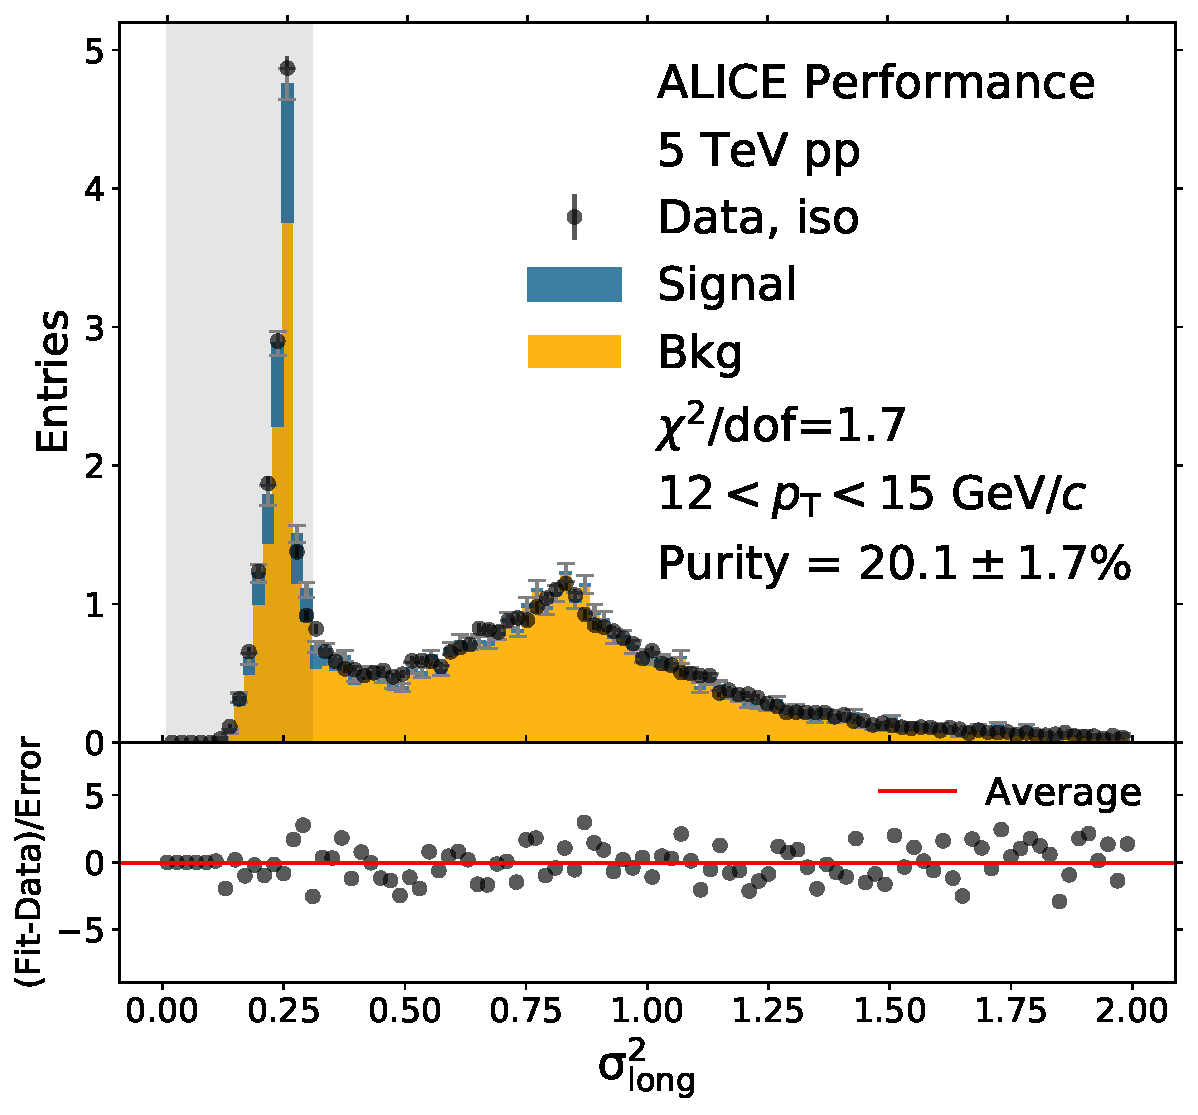
\includegraphics[width=0.3\textwidth]{Data_Analysis/Purity/tf-example-pp-cluster_Lambda-12-15.pdf}
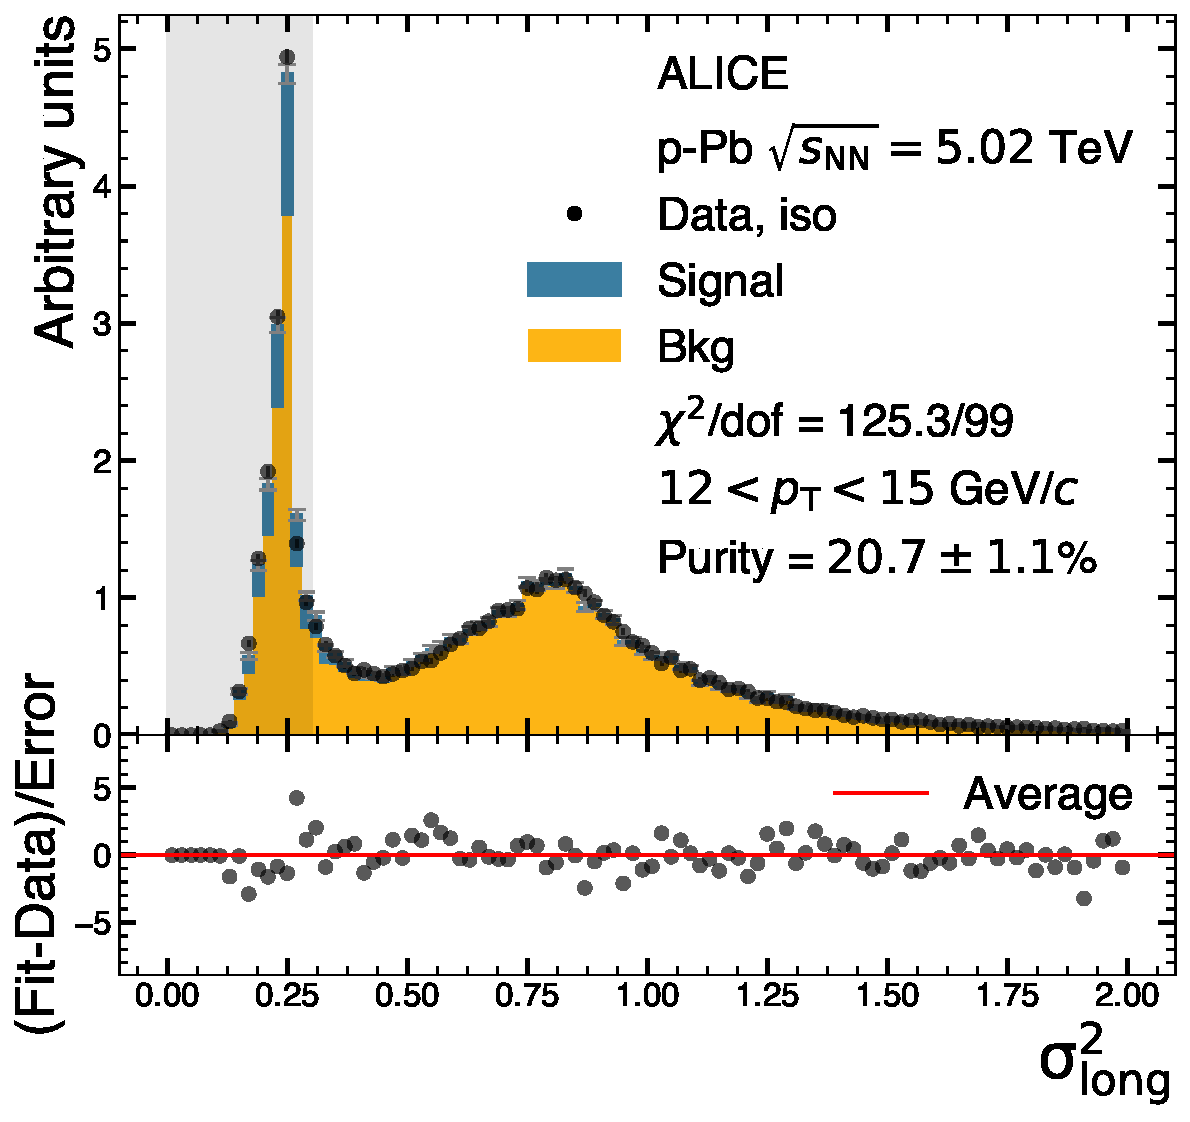
\includegraphics[width=0.3\textwidth]{Data_Analysis/Purity/tf-example-p-Pb-cluster_Lambda-12-15.pdf}
\\
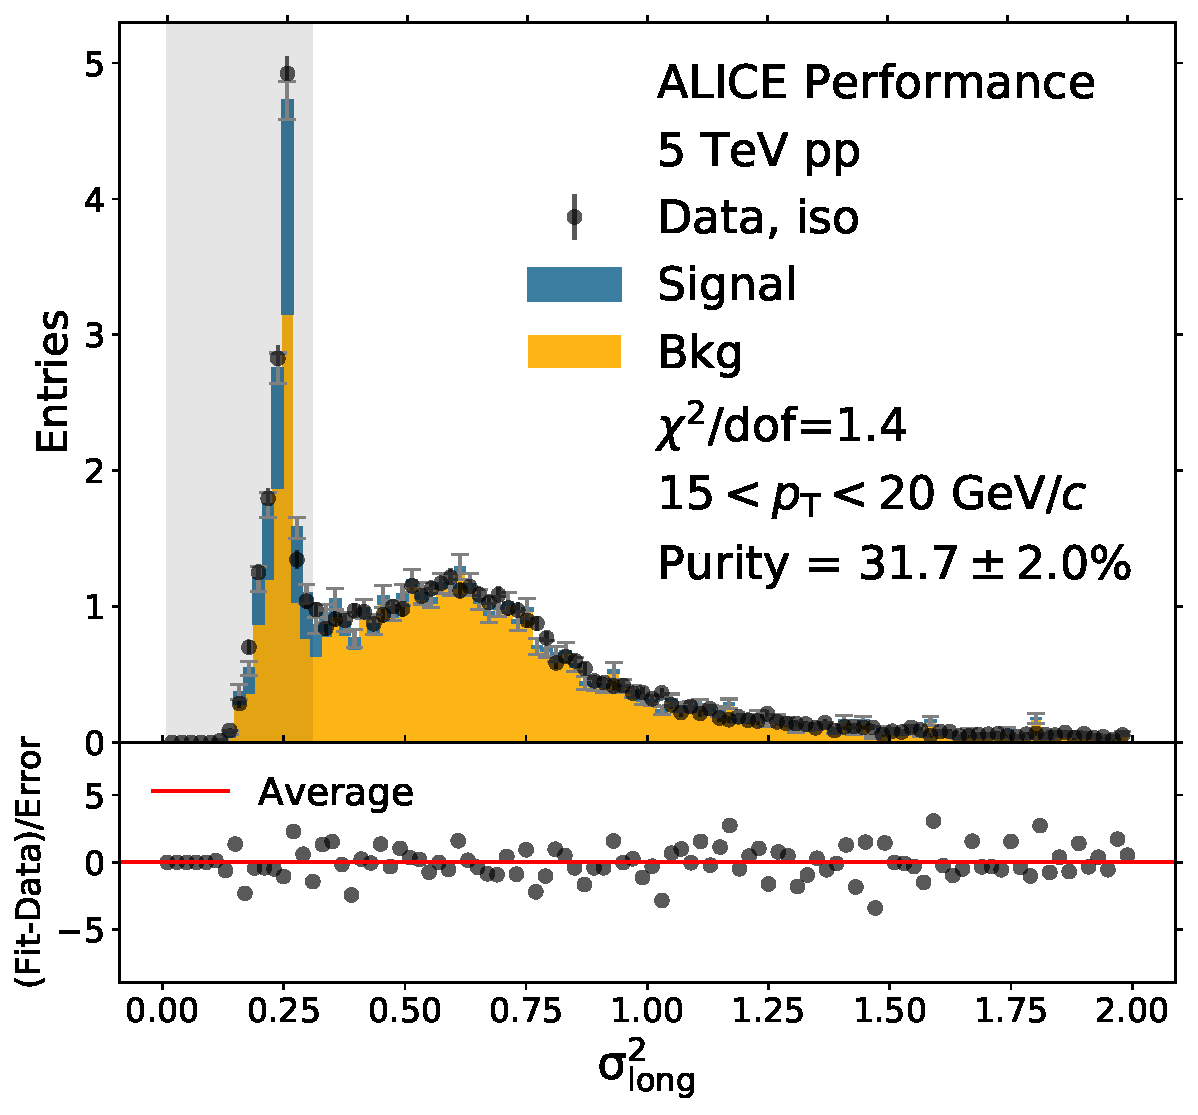
\includegraphics[width=0.3\textwidth]{Data_Analysis/Purity/tf-example-pp-cluster_Lambda-15-20.pdf}
\includegraphics[width=0.3\textwidth]{Data_Analysis/Purity/tf-example-p-Pb-cluster_Lambda-15-20.pdf}
\\
\includegraphics[width=0.3\textwidth]{Data_Analysis/Purity/tf-example-pp-cluster_Lambda-20-25.pdf}
\includegraphics[width=0.3\textwidth]{Data_Analysis/Purity/tf-example-p-Pb-cluster_Lambda-20-25.pdf}
\\
\includegraphics[width=0.3\textwidth]{Data_Analysis/Purity/tf-example-pp-cluster_Lambda-25-40.pdf}
\includegraphics[width=0.3\textwidth]{Data_Analysis/Purity/tf-example-p-Pb-cluster_Lambda-25-40.pdf}
\caption{\lambdasquare distribution of isolated clusters (black) and template fit results for \pPb~data in various \pt~ranges. The stacked histograms (yellow for background, blue for signal) show the predicted counts corresponding to the best fit. The bottom panels show the normalized residuals of the fit, with the statistical uncertainty on the isolated cluster data and the background template added in quadrature. The gray shaded region indicates the signal region for the isolated-photon selection. See text for additional details.}
\label{TemplateFit}
\end{figure}

%\begin{table}
%   \caption{Impact of the \gammaiso selection variations on purity measurement on pp and \pPb~data. The nominal isolation selection is changed to $\iso<$1.50 $\pm$ 0.25 \GeVc; the nominal shower-shape selection is changed to  $\lambdasquare<0.30 \pm 0.03$}
%   \label{tab:variationspurity}
    % \begin{tabular*}{1.0\columnwidth}{@{\extracolsep{\fill}}l|llllll@{}}
    % 	\hline
    % 	 & Nominal & $\iso < 1.25$ \GeVc & $\iso < 1.75$ \GeVc & $\lambdasquare < 0.27$ & $\lambdasquare < 0.33$ \\
    % 	\hline
    % 	pp data & & & & & \\
    % 	\hline
    % 	12--15 \GeVc & 16.9 & 18.2 & 15.9 & 16.5 & 16.9 \\
    % 	15--20 \GeVc & 29.5 & 31.0 & 28.0 & 29.3 & 29.1 \\
    % 	20--25 \GeVc & 46.8 & 48.4 & 45.4 & 49.1 & 44.9 \\
    % 	25--40 \GeVc & 48.0 & 49.3 & 46.7 & 55.9 & 45.1 \\
    % 	\hline
    % 	p-Pb data & & & & & \\
    % 	\hline
    % 	12--15 \GeVc & 20.7 & 21.5 & 19.7 & 20.2 & 20.5 \\
    % 	15--20 \GeVc & 34.2 & 35.5 & 33.1 & 34.3 & 33.6 \\
    % 	20--25 \GeVc & 47.6 & 49.0 & 46.5 & 51.7 & 44.9 \\
    % 	25--40 \GeVc & 54.6 & 56.8 & 52.8 & 62.1 & 51.1 \\
    % 	\hline
    % \end{tabular*}
%\end{table}


\begin{figure}[h]
\center
\includegraphics[width=0.8\textwidth]{Data_Analysis/Purity/purity.pdf}
\caption{Purity of the $\gammaiso$ sample as a function of transverse momentum for pp (red) and \pPb~(blue) data. The error bars represent statistical uncertainties only. The red shaded area represents systematic uncertainties in pp, while the blue empty boxes represent systematic uncertainties in \pPb. The smooth lines correspond to a three-parameter error function fit to the data.}
\label{fig:purityresults}
\end{figure}

The purities in the pp and \pPb~datasets are compatible within the uncertainties. The $\text{Weights}(\lambdasquare)$ function for different \pt~ranges is shown in Appendix~\ref{sec:MCbasedcorrection} and the evaluation of the systematic uncertainty associated with this correction is described in Section~\ref{sec:puritysystematics}. 
\FloatBarrier
%%%%%%%%%%%%%%%%%%%%%%%%%%%%%%%
% \subsection{Systematic uncertainties of the purity measurement}


% \section{Particle Selection}

% \subsection{Photon Selection}
% \label{sec:photon_selection}
% \subsection{Charged Hadron Selection}
\section{Charged Particle Tracking}
\label{sec:tracking}
The detectors usually responsible for measuring the charged hadrons in this analysis are the ALICE Inner Tracking System (ITS) and Time Projeciton Chamber (TPC). During the 13def and 17q periods, however, the TPC was either not read out or compromised due to space-charge distortions, mentioned in Sec.~\ref{sec:tpc}. As a result, this analysis relies on only the ITS for track reconstruction.

ITS-only tracking in ALICE is new for this flavor of analysis. As a result, the charged-particle $\pt$-spectrum using ITS-only tracking is compared to the normal TPC+ITS tracking in the data-taking period when the TPC was active and free of space-charge distortions (the low-luminosity 13b data-taking period at 5 TeV \pPb~minimum-bias data) as well as with published ALICE measurements~\cite{Acharya:2018qsh} that use the same dataset (a more thorough comparison to published ALICE data is done in Sec.~\ref{sec:tracking_published_comparision}).

The combined effect of tracking efficiency, fake rate, and track momentum smearing corrections are calculated using MC simulations, and validated by the comparison to the established hybrid-tracking method in ALICE. The comparison to hybrid tracking also serves as an estimate of the systematic uncertainties due to mis-modeling of the tracking performance.

To study the performance of ITS-only tracking, minimum bias \pPb~events for both data and Monte Carlo. The Monte Carlo simulations used for this section are LHC13b2\_efix\_p1, a \textsc{DPMJET} simulation anchored to LHC13b,c and LHC17l3b, a pp \textsc{Pythia8} simulation anchored to LHC17p. The events are sampled from the LHC13b period and the datasets from \cite{Acharya:2018qsh}, as mentioned previously. Only events with the minimum bias trigger (CINT7) that also the vertex and pileup selections described in Section~\ref{sec:eventselection}. The tracks reconstructed from the ITS (''ITS-only tracks''), are compared with tracks reconstructed from information obtained from both the TPC and ITS (''TPC+ITS tracks'', or ''hybrid'' tracking). Here, ITS-only tracks are reconstructed in a \textit{stand-alone} way and are not simply the ITS-segment of a ITS+TPC track.

In order to select good-quality tracks emerging from the primary vertex while maintaining a high efficiency, each track is required to satisfy the cuts summarized in Table ~\ref{tab:track_cuts}. A set of standard PWG-JE cuts are applied to all tracks, and additional track cuts are applied depending on whether the track is a TPC+ITS track or an ITS-only track. 

\begin{table}[h]
   \centering
      \caption{Summary of the cuts used in Track Selection.}	
   \label{tab:track_cuts}
   \begin{tabular*}{1.0\columnwidth}{@{\extracolsep{\fill}}l|c@{}}
      	\hline
 		\textbf{Common Cuts}\\
        %\textbf{ITS--Only Cuts}\\
        \hline
        track $\eta$ & $|\eta| < 0.8$\\
        track $\pt$ & $\pt \geq 0.150$ \GeVc\\
        SetMaxDCAToVertexXY & 2.4 cm\\
        SetMaxDCAToVertexZ & 3.2 cm\\
        SetDCAToVertex2D & TRUE\\
		\hline \hline
        \textbf{TPC+ITS Cuts}\\
        \hline
        SetMinNClustersTPCPtDep & 70.+30./20.*x, 20.0\\ 
        SetMinNClustersTPC & 70\\
        SetMaxChi2PerClusterTPC & 4\\
        SetMaxChi2PerClusterITS & 36\\
        SetMaxFractionSharedTPCClusters & 0.4\\
        SetMaxChi2TPCConstrainedGlobal &36 \\
        SetRequireTPCStandAlone & TRUE\\
        SetRequireTPCRefit & TRUE \\
        SetRequireITSRefit & TRUE\\
        SetRequireSigmaToVertex & FALSE \\
        SetAcceptKinkDaughters & FALSE\\
        \hline \hline
        \textbf{ITS--Only Cuts}\\
        \hline
        SetRequireITSPureStandAlone &TRUE\\
        SetMinNClustersITS & 4\\
        SetMaxChi2PerClusterITS & 36\\
        \hline
   \end{tabular*}
\end{table}
\FloatBarrier

\subsection{Efficiency and Fake Rate}
\label{sec:Efficiency_fake_rates}
%The tracking efficiency is calculated from the minimum bias \pPb~simulation (see Table~\ref{tab:MCsamples}).
The tracking efficiency is calculated as the ratio of the number of reconstructed primary particles\footnote{No special tuning of the particle type composition is performed. This typically only matters at low $\pt$ and enforces a small (percent level) correction to the out-of-the-box results.}, $N_{\mathrm{prim,rec}}(p_\mathrm{T})$, to the number of generated primary particles, $N_{\mathrm{prim,gen}}$. The truth-to-reconstructed matching is done following the standard ALICE method.
\begin{equation}\label{eq:eff}
\epsilon (\pt^{\mathrm{true}}) = \frac{N_{\mathrm{prim,rec}}(\pt^{\mathrm{true}})}{N_{\mathrm{prim,gen}}(\pt^{\mathrm{true}})}.
\end{equation}

Shown in Eq.~\ref{eq:eff}, the simulated or ''truth'' transverse momentum, $\pt^{\mathrm{true}}$, is used in both the numerator and denominator in order cancel effects of efficiency from bin-migration due to momentum smearing.

The numerator of Equation~\ref{eq:eff} is restricted for charged particles with generated pseudorapidity in the range $|\eta^{\mathrm{true}}|<0.8$ and azimuth $0<\varphi^{\mathrm{true}}<2\pi$. Therefore, the correction factor accounts for both geometrical acceptance, detector inefficiencies, and dead channels.  

Fake tracks are defined as reconstructed tracks that do not match to a truth particle. The fake rate is calculated by taking the ratio of the number of fake tracks to the total number reconstructed tracks. It is parametrized as a function of the reconstructed transverse momentum of the track, $\pt^{\mathrm{reco}}$:

\begin{equation}\label{eq:fakes}
\mathrm{fake rate} (\pt^{\mathrm{reco}}) = \frac{N_{\mathrm{unmatched}}(\pt^{\mathrm{reco}})}{N_{\mathrm{all reco}}(\pt^{\mathrm{reco}})}.
\end{equation}

Figure~\ref{fig:tpcEff} shows the efficiency and the fake rates for the TPC+ITS and ITS only tracks. In both cases the efficiency grows with $\pt$ up to about 1 \GeVc~where it dips and it reaches a plateau value with no significant $\pt$ dependence. The efficiency starts at about 57$\%$ for the TPC+ITS tracks and at 70$\%$ for ITS-only tracks at 150 MeV and plateaus at 84\% and 88\% respectively. %The plateau is calculated by applying a constant fit from {2 $< \pt <$$ 20 GeV/c$}. 

The lower efficiency for the TPC+ITS tracks compared to ITS-only tracks is expected since the former requires a matching between ITS and TPC track segments, which has some inefficiency. This study shows that the matching efficiency is high at large $\pt$ but leads to substantial differences at low $\pt$.  

%The decrease in the tracking efficiency by about 2--5$\%$ in the range 1--3 \GeVc~is due to the fact that above about 1 \GeVc, tracks are almost straight and can be contained completely in the dead areas between TPC sectors or in ITS dead staves. Therefore, at high $\pt$ the efficiency is dominated by geometry and thus has a constant value.

The fake rate for the TPC+ITS tracks is less than a percent over the entire range shown. In comparison, the fake rate is larger in the ITS-only tracks. It is below 5\% up to 5 \GeVc, and it grows roughly linearly and reaches 15\%  at 10 \GeVc. The higher fake rate is due to the much lower number of clusters associated with ITS-only tracks (maximum of 6) than to TPC+ITS tracks (minimum of 70).
\begin{figure}[h]
\center
\includegraphics[width=0.7\textwidth]{Data_Analysis/Tracking/HybridAndITS_Eff_fakerate_pPb_lowpt.pdf}
\caption{Efficiency and fake rate for combined TPC+ITS tracking (filled circles) and ITS-only tracking (open circles) obtained with \pPb~simulation. The error bars represent statistical uncertainty only.}
\label{fig:tpcEff}
\end{figure}

%The efficiency and fake rate between pp and \pPb~are rather similar. Figure~\ref{fig:ppPb_eff} shows the comparison between the pp efficiency and \pPb~efficiency as well as the fake rate for pp and the fake rate for \pPb~for ITS-only tracks. The pp efficiency was calculated using the 17l3b Monte Carlo simulation. %The pp efficiency plateaus at 85\%, while the \pPb~efficiency is 88\% as mentioned previously. 
%\begin{figure}[h]
%\center
%\includegraphics[width=0.7\textwidth]{Tracking/EfficiencyFakeRate_tracking_pApp_compare_halfGeV20GeV_publishedBinning.pdf}
%\caption{Efficiency and fake rate comparison between pp and \pPb~ITS-only tracks. The error bars represent statistical uncertainty only. }
%\label{fig:ppPb_eff}
%\end{figure}
\FloatBarrier

\subsection{Resolution, Response Matrix and Bin Migration}
The main difference between TPC+ITS and ITS-only tracking lies in the much worse momentum resolution of the latter. This is driven by geometry 
and $\int Bdl$ as the TPC covers up to {$z=$258 cm} but the ITS only to {$z=$48 cm}. 

Figure~\ref{fig:resolution} shows the momentum resolution as a function of $\pt^{\mathrm{true}}$ for 
TPC+ITS and ITS-only tracks. The momentum resolution of both increases with \pt; however, the resolution for TPC+ITS never exceeds a relative 2\% below 20 \GeVc, while the ITS-only tracking resolution is about a factor of 7 worse and reaches $\sim$15\% by 10 \GeVc. In both cases the resolution curves have the expected shape: the growth at low momentum is due to multiple-scattering and the linear growth at higher $\pt$ arises from the number and depth of position measurements, and the track bend at the measurement planes. 
\begin{figure}[h]
\center
\includegraphics[width=0.7\textwidth]{Data_Analysis/Tracking/HybridAndITS_resolution_lowpt.pdf}\\
\caption{The relative $\pt$ resolution for TPC+ITS tracking and ITS only tracking. The error bar represents statistical uncertainty only.}
\label{fig:resolution}
\end{figure}

The tracking response matrix is defined as the correlation between the reconstructed and generated transverse momentum. This matrix is filled only for reconstructed tracks with a true match; fake tracks are explicitly excluded. Figure~\ref{fig:responseMatrixTPC} shows the response matrix, its one-dimensional projections, and the ratio of true to reconstructed spectra. The ratio of the true to reconstructed spectra is used to correct for bin migration effects, where a track is placed in the wrong \pt bin due to the finite momentum resolution of the detector:

\begin{equation}\label{eq:bin_migration}
\mathrm{bin\:migration} (\pt^{\mathrm{reco}}) = \frac{N_{\mathrm{prim,reco}}(\pt^{\mathrm{true}})}{N_{\mathrm{prim,reco}}(\pt^{\mathrm{reco}})}.
\end{equation}

\begin{figure}[h!]
\includegraphics[width=0.98\textwidth]{Data_Analysis/Tracking/Matrix_tracking_tpc_MBMC_0GeV15GeV_dNdPt.pdf}\\
\includegraphics[width=1.0\textwidth]{Data_Analysis/Tracking/Matrix_tracking_its_MBMC_0GeV15GeV_dNdPt.pdf}

\caption{Left panel: correlation matrix between true $\pt$ and reconstructed $\pt$ of tracks reconstructed with TPC+ITS (upper row) and ITS-only (bottom row). Middle panel: projections of the response matrix into the true and reconstructed $\pt$. Right panel: ratio of true to reconstructed spectra. This ratio used as part of the bin-by-bin correction factors.}
\label{fig:responseMatrixTPC}
\end{figure}

The effect of momentum smearing on tracks is clearly visible in the projection plots, where the reconstructed spectrum is significantly harder at high $\pt$. The ratio of truth to reconstructed $\pt$ is very close to unity in the TPC+ITS case, as expected. On the other hand, the ratio deviates significantly from unity in the ITS-only case; it reaches 0.9 at 6 \GeVc~and drops quickly, reaching 0.5 at about 13 \GeVc. The quick drop at high $\pt$ comes mainly from the linear degradation of the relative momentum resolution combined with the fast drop of the true spectrum to produce large effects in the tails. 

The bin migration (b), along with the tracking efficiency ($\epsilon$) and the fake rate (f) are used as the correction factor equation~\ref{eq:track_weight} for the charged hadron tracks; all of them are shown together in Figure~\ref{fig:correctionFactors}. Based on overlapping plot of pp and \pPb, we can see that correction factors are similar for tracks from a pp collision or a \pPb~collision. We conclude that the multiplicity in \pPb~is low enough such that it does not affect tracking performance.  

\begin{equation}\label{eq:track_weight}
w = \frac{1}{\epsilon}(1-f)b
\end{equation}

\begin{figure}[h]
\center
%\includegraphics[width=.45\textwidth]{Data_Analysis/Tracking/trackCorrectionFactors_pp.pdf}
%\includegraphics[width=.45\textwidth]{Data_Analysis/Tracking/trackCorrectionFactors_pPb.pdf}
\includegraphics[width=.7\textwidth]{Data_Analysis/Tracking/trackCorrectionFactors_pPbAndpp.pdf}
\caption{The efficiency, fake rate, and momentum smearing correction factors for pp and \pPb~data.}
\label{fig:correctionFactors}
\end{figure}

\FloatBarrier

\subsection{Angular Dependence of Tracking Efficiency}
The 2D $\varphi$-$\eta$ efficiency is calculated in a similar way to the $\pt$ efficiency described in Equation~\ref{eq:eff}, but instead of being functions of $\pt^{\mathrm{true}}$, the efficiency is a function of the true azimuthal angle and pseudorapidity, $\varphi^{\mathrm{true}}$ and $\eta^{\mathrm{true}}$ respectively. Only tracks with {$\pt^{\mathrm{true}}>1$} \GeVc~are considered to avoid tracks with sharp bends in the magnetic field that would obscure the impact of dead regions.

\begin{figure}[h]
\center
\includegraphics[width=0.46\textwidth]{Data_Analysis/Tracking/etaPhi_eff_tpc.pdf}
\includegraphics[width=0.46\textwidth]{Data_Analysis/Tracking/etaPhi_eff_4layers.pdf}
\caption{Tracking efficiency as a function of $\varphi^{\mathrm{true}}$ and $\eta^{\mathrm{true}}$ for TPC+ITS (left) and ITS-only (right) tracks.}
\label{fig:2Defficiency}
\end{figure}

Figure~\ref{fig:2Defficiency} shows the resulting efficiency for TPC+ITS and ITS-only tracks. While the TPC+ITS 2D $\varphi$-$\eta$ distribution looks uniform, this is not the case for the ITS-only distribution, which has visible dips in the efficiency at various $\varphi$. The efficiency is close to unity for most of the phase space covered. There are no big $\eta$ variations, but there are large $\varphi$ variations. The efficiency holes at $\varphi$ = $-$0.8 and $-$0.2 are very visible and reach values close to zero. These are attributed to ITS-staves that are completely dead. Any variations in $\varphi$ in the $\gammaiso$-hadron analysis are corrected for using the event mixing technique described in Section \ref{sec:EventMixing}
\FloatBarrier



\section{Photon Hadron Correlations}


In this study, the exact cross section of isolated photons is not the observable, nor is the cross section of charged hadron production in a given event. The quantity of interest is the number partner particles associated with those trigger photons, relating to the leading order picture of back-to-back prompt photon and parton. Therefore, instead of quoting the absolute yield of pairs, it is useful to divide by the number of triggers to obtain the conditional yield (also called per-trigger yield) of associated hadrons. This quantity is typically plotted as a function of the azimuthal angle between the trigger and partner particle, \deltaphi:

\begin{equation}
	\deltaphi \equiv \phi^\mathrm{cluster} - \phi^\mathrm{track}
\end{equation}

 The \deltaphi~distribution of cluster-track pairs, divided by the number of triggers is defined as the trigger normalized correlation function, $C$:

\begin{equation}
\label{eq:basic_correlation}
	C \equiv \frac{P}{T}
\end{equation}

Where $T$ is simply the number of triggers, and $P$ is the \deltaphi~distribution of cluster-track pairs. Such distributions often highlight the structure of jets. They typically contain a large, very narrow peak at $\deltaphi=0$, arising from the autocorrelation of the particles within an jet, and a broader peak centered at $\deltaphi=\pi$ arising from the correlation between two jets in the event, shown in Fig.~\ref{fig:dihadron_cartoon}. 

Enforcing an isolation requirement will heavily suppress the near side peak, however. The near side peak is further removed after the decay photon hadron correlation is subtracted, likely removing the remaining contribution of background jets to the isolated photon triggers \ref{sec:decay_photon_subtraction}. This becomes particularly important for the underlying event estimate detailed in \ref{sec:ue_subtraction_correlations}

%TODO fix ue_subtraction_correlations reference

At lowest order in QCD, prompt photons exactly balance the hard scattered parton in the event. For this reason, studies of photon-tagged jets and jet fragments have been dubbed the "golden channel" for studying parton. %Save for correlations section

%Low energy jets are of particular interest as they are less time dilated, and thus the timescale of fragmentation is comparatively less compared to higher energy jets. By studying jet fragments...

%We actually get an extremely inclusive sample of jets. One needs to make the argument first that jets are a quickly spectrum in pT. If so, then we can only really make an argument on jets around the mean of the distribution.
Eq.~\ref{eq:basic_correlation} is closely related to Eq.~\ref{eq:yield}. The former can be thought of as an ingredient to the latter; Eq.~\ref{eq:basic_correlation} refers to the correlation function over the full range of \deltaphi, while Eq.~\ref{eq:yield} refers to the yields, often the result of integrating $C$ at large  $\deltaphi$.

\subsection{Signal Correlation Function}


%TODO edit this with the equations from the note

\begin{comment}
	In this section we present the method we use to extract \gammaiso-hadron azimuthal correlations. We select tracks with $|\eta|<0.8$ and $0.5 <\pttrack < 10$ \GeVc, following the studies shown in Section~\ref{sec:tracking}. We only consider cluster-track pairs within $|\Delta \eta| < 1.2$. Our cluster \pt~range selection is $12 < \ptcluster< 40\ \GeVc$, with isolation criteria of $\iso < 1.5\ \GeVc$. We apply the same track selection criteria described in Section~\ref{sec:tracking}, Table \ref{tab:track_cuts}. We present our results as a function of \zt, which is defined as:
 \begin{equation}
\zt = \frac{\pttrack}{\ptcluster}
 \end{equation}

Section~\ref{sec:decaybkgsubtraction} shows the way we correct for the impurity of our \gammaiso selection; Section~\ref{sec:EventMixing} describes the pair-acceptance correction obtained with the event-mixing method.


\subsection{$\ydecay$ background Subtraction}
\label{sec:decaybkgsubtraction}
We split the clusters that pass our $\iso<1.5 $ GeV selection in two regions of interest, our signal region \(SR\) with the selection $\lambdasquare<0.3$, and our background region, \(BR\) as $\lambdasquare>0.4$ 

\end{comment}

Section \ref{sec:photons} introduced isolated prompt photons as the primary photon signal for this measurement. However, as detailed in \ref{sec:purity}, there is a substantial amount of background contributing to \gammaiso candidates and a subsequent contribution to the \gammaiso-hadron correlations. In this section, we the disentangle the signal of this measurement from what is initially measured.\\ 

We directly measure the trigger-normalized correlation of shower signal region isolated clusters and associated hadrons, \CSR. This quantity will be made up of the true signal correlation function, \CS~-- the correlation of isolated prompt photons and associated hadrons from the recoiling parton-- as well as the true background correlation, \CB, predominantly arising from the correlation between decay photons that pass the cluster selection and hadrons. We call this background the correlated background, as it arises from the correlation of background photons and the hadrons in the event. To separate what is initially measured, \CSR, and the true signal, \CS, we begin by taking a look at the ingredients of \CSR. First, we denote the number of trigger clusters in the shower signal region, also called the number of \gammaiso candidates, \TSR. We can write \TSR~as:
%TODO Fix reference for shower shape ranges
\begin{equation}
\label{eq:TS_TB}
\TSR = \TS + \TB.
\end{equation}

Here we define \TS~as the number of "true" signal triggers (i.e. the number isolated prompt photon triggers) and \TB~as the background, most prominently decay photons that pass our $\gammaiso$ selection. Similarly, the \deltaphi~distribution of signal region cluster-track pairs, \PSR~ can be written as:
\begin{equation}
\label{eq:PS_PB}
\PSR = \PS + \PB.
\end{equation}

Now, following the notation of Equation \ref{eq:basic_correlation}, we can write the  trigger-normalized correlation functions for shower signal region clusters as:
\begin{eqnarray}
\label{eq:CSR}
\CSR &=& \frac{1}{\TSR}\PSR.
%\CBR &=& \frac{1}{\TBR }\PBR.
\end{eqnarray}
These quantities are directly measured. Similarly, we can write the true signal and true background correlation functions:
\begin{eqnarray}
\CS &=& \frac{1}{\TS}\PS\\\label{eq:CS}
\CB &=& \frac{1}{\TB}\PB\label{eq:CB}
\end{eqnarray}

The goal of this formalism is to write the true signal correlation function (\CS)~in terms of quantities that are measured --  \CSR~and the measured purity, $p$. To this end, the next step is to write the measured quantity, \CSR, in terms of true signal and true background correlation functions:
 
\begin{eqnarray}
\label{eq:31}
\CSR &=& \frac{1}{\TSR}\PSR = \frac{1}{\TSR}(\PS + \PB)\\
\CSR &=& \frac{1}{\TSR}(\TS\CS +\TB\CB)\label{eq:CSR_TS_TB}
\end{eqnarray}

Where we have substituted equation \ref{eq:PS_PB} into  Equation \ref{eq:CSR}, followed by using Equations \ref{eq:CS} and \ref{eq:CB} to substitute out \PS~and \PB, respectively. \TS~ and \TB~ are not directly measured, however they can be expressed in terms of measurable quantities. The purity is defined as the fraction of true signal in our \gammaiso clusters, or in other words, $p \equiv \TS/\TSR$~(see Section~\ref{sec:purity}). Substituting this into equation \ref{eq:TS_TB} and solving solving for \TB/\TSR, one obtains: $\TB/\TSR = 1-p$. This a natural result of the definition of purity: If $p$ is the fraction of the true signal making up the \gammaiso candidates, $1-p$ must be everything else, i.e. background. To summarize:

\begin{eqnarray}
	p &\equiv & \TS/\TSR\\
	1-p &=& \TB/\TBR
\end{eqnarray}


Substituting $p$ into Equation \ref{eq:CSR_TS_TB}:
\begin{equation}
	\CSR = p\CS+ (1-p)\CB \label{eq:CSR_CS}
\end{equation}

Finally, we can solve for \CS~in terms of \CSR~and $p$:
\begin{equation}
\CS = \frac{\CSR - (1-p) \CB}{p}
\label{eq:FinalSubtraction_CB}
\end{equation}


Equation \ref{eq:FinalSubtraction_CB} shows \CS~in terms of the measured quantities, \CSR~and the purity. It also includes, however, a term for the background correlation function \CB, that cannot be determined from \CSR and the purity alone. The correlation function \CB is described in more detail in section \ref{sec:cb}.

\subsection{Decay Photon Hadron Correlations}
\label{sec:cb}

There is a large fraction of \ydecay background within the isolated photon sample, and a subsequent $\gamma^\mathrm{decay}$-hadron correlation present in the measured correlation function. The correlation between hadrons and background photons within the \gammaiso sample, most prominently photons from neutral meson decays, correspond to the \CB~term in in Equation \ref{eq:FinalSubtraction_CB}. While the equation gives us the scale of this background, $1-p$, it does not offer information on the shape of this \deltaphi distribution. To understand the shape, we take advantage of the fact that the most prominent source background photons within the \gammaiso population are photons from neutral meson decays. Outside of the \gammaiso selection, these photons tend to have more assymmetric shower profiles, and thus larger values of \lambdasquare. Therefore, in order to select on clusters arising from decay photons, an inverse shower shape selection is applied which we define as the shower background region, BR:

\begin{equation}
	\label{eq:BR}
	\lambdasquare(\mathrm{BR}) > 0.4
\end{equation}

Thus, in order to approximate \CB, a \ydecay hadron correlation function is measured by taking the correlation of clusters in the shower background regions with associated hadrons in the event. This shower background region correlation function, much like Eq. \ref{eq:CSR} is defined as \CBR:
\begin{equation}
\CBR = \frac{1}{\TBR}\PBR.
\end{equation}

With \TBR as the number of clusters in the shower background region, and \PBR~as the \deltaphi~distribution of shower background region clusters and hadrons.\\

Notably, because the underlying physics process that dictates the number and distribution of correlated pairs is independent of the opening angle of the neutral-meson decay, which is what drives the shower-shape, the approximation $\CBR \approx \CB$ can be made.\footnote{Here again we take advantage of trigger normalized quantities. The number of isolated photons in the shower background region vastly outnumber the number of isolated photons within the shower signal region. By focusing on the associated yield of hadrons per each photon, which is not correlated with \lambdasquare, this very useful approximation can be made.} In other words, the shower background region correlation function is a good approximation of the correlated background that contributes to the shower signal region correlation function, \CSR. Therefore, Eq. \ref{eq:FinalSubtraction_CB} can be re-written:
\begin{equation}
\CS = \frac{\CSR - (1-p) \CBR}{p}
\label{eq:FinalSubtraction}
\end{equation}

As a result, the true signal correlation function, \CS, is finally written in terms of measurable quantities: The shower signal region correlation function, \CSR, the purity, p, and the newly defined shower background region correlation function (or \ydecay correlation), \CBR.

Thus, hadrons are correlated with clusters in the shower background region to directly measure the \ydecay-hadron correlation functions. This \ydecay-hadron correlation function is then subtracted from the the shower signal region correlation function to obtain the signal correlation. This scaling, however, must be done carefully due to the \pt~dependance of the purity. The next few sections describe corrections to the correlation functions. Unless explicitly stated, these corrections (purity weighting, acceptance corrections, and charged particle tracking corrections) are applied to both the \CSR and \CBR before the two are finally subtracted in Sec.~\ref{sec:decaybkgsubtraction}


%where we have made the approximation that \CB~ (per-trigger pairs for decay photons that pass our $\gammaiso$ selection) can be approximated by the measured \CBR~(per-trigger pairs for decay photons that pass our isolation criteria but not our shower-shape selection). This is justified because the underlying physics process that dictates the number of correlated pairs is independent from the opening angle of the neutral-meson decay, which is what drives the shower-shape.
       
%This scaling, however, must be done carefully due to the \pt dependance of the purity

%TODO Final subtraction error propagation. Articulate the point that CSR and CBR are calculated independantly
%TODO include gaussion error propagation calculation. Point out that this overestimates the uncertainty, as there is a clear correlation in applynig the purity to CBR and CSR. Show what's done instead.


%The correlated background subtraction detailed in Equation~\ref{eq:FinalSubtraction} assumes that the decay-photon hadron correlation we directly measure, \CBR, is an accurate estimation of the decay-photon hadron correlation that pollutes signal region. In principle, the decay photons from neutral-meson decays that pass the shower shape cut may be biased toward pairs with a smaller opening angle (larger cluster \pt). We checked this by forcing the \pt distributions in \CSR and \CBR. 


\subsection{Photon Purity Weighting}

%The \ydecay-hadron correlations is scaled according to the purity, in this case $1-p$ and subtracted. %With the purity quantifying the fraction of true signal present in \gammaiso candidates, $1-p$ indicates the fraction of background.
Equation \ref{eq:FinalSubtraction} shows the background correlation function, \CB, approximated by the \ydecay~correlation function, and scaled by $1-p$ according to its relative contribution measured correlation function. The purity is a \pt dependent quantity, rising quickly with \pt, correlations using a low-\pt~cluster have a higher fraction of background than high-\pt~clusters (see Figure \ref{fig:purity}). As a result, measuring the \ydecay-hadron correlation function for all clusters and scaling by the mean of the purity would lead to and underestimation of the background at low \ptcluster, and an overestimation at high \ptcluster. This has will have a non-trivial effect on the corresponding \zt~bins, which include clusters with a wide range of \ptcluster. Additionally,  Equation \ref{eq:FinalSubtraction} includes an overall scale of 1/$p$ in order to obtain the correct conditional yield of hadrons after the subtraction in the numerator, and will yield similar complications if applied correlations using clusters over the full \ptcluster~ range.\\

In order to avoid these complications, clusters are weighted by the purity corresponding to their exact \ptcluster~when constructing the correlation functions. In order to capture the quickly rising behavior of the purity at low \ptcluster, the purity is fit to a 3-parameter error function. This fit to the purity is shown in Figure \ref{fig:Purity_Error_Function}The \ptcluster becomes an input to this function, and precise purity weighting is applied precisely to each cluster. 

\begin{figure}
	\label{fig:Purity_Error_Function}
	\includegraphics[width=0.5\textwidth]{Data_Analysis/Error_Function_Fits/pp_Mean_Center}
	\includegraphics[width=0.5\textwidth]{Data_Analysis/Error_Function_Fits/pPb_Mean_Centers}
  \caption{A 3-parameter error function is fit to the purity values measured in pp (left) and \pPb~(right) data. The width of the band represents the uncertainty on the fit.}
\end{figure}


According to Equation \ref{eq:FinalSubtraction}, the overall purity weights will be $1/p$ and $(1-p)/p$ for shower signal and shower background region clusters, respectively. 

\subsection{Track Efficiency, Fake Rate, and Bin Migration Weights}
In order to correct for the tracking efficiency, fake rate, and bin-migration we apply a track-by-track weighting according to:

\begin{equation}
w_{\mathrm{tracking}}(\pt^{\mathrm{track}}) = \frac{1}{\epsilon}\times(1- f)\times b.
\end{equation}

Here $\epsilon$ is the track efficiency, $f$ is the fake rate, and $b$ is the bin-to-bin migration correction. These are described in Section~\ref{sec:tracking}. The corrections are estimated independently for pp and \pPb~data although the performance is very similar. The weights are applied to the measure charged hadrons as the correlation functions are being constructed, analogous to how the purity weighting is applied to the photons in the correlations functions.

\subsection{Pair-Acceptance Correction with Event Mixing}

\label{sec:EventMixing}
%TODO: Add reference to detector setup, and point out the acceptance of EMCal and ITS
Initially, two particle correlations consist of a combination of true physical correlations and detector effects. The detector effects result from inefficiencies and limited acceptance in the detectors. The study of trigger normalized yields of associated hadrons eliminates the need to correct for isolated cluster efficiency, and Section \ref{sec:tracking} outlines the charged tracking efficiency correction. %TODO: Fix Tracking Reference.

The remaining detector effect on the correlations are pair-acceptance effects:
correlations are constructed through pairs of clusters and charged tracks. This results in a convolution of acceptance effects from the limited acceptance of EMCal and ITS, which we call pair acceptance effects. These effects are corrected for by using the event mixing technique. Event mixing is a data driven approach to correcting for detector acceptance effects \footnote{Event mixing is also used for estimating combinatorial background.}. By constructing observables with particles from different events, we remove true physics correlations from the correlation functions, isolating detector effects from limited acceptance in \(\eta\) and detector inhomogeneity in $\eta$ and $\varphi$. 


Cluster-track pairs in same event correlation functions obviously share the properties of the event, and such properties often effect detector response. In order to make the mixed-event correlations as analogous as possible to the to same-event correlation functions, events that are as similar as possible with respect to these event properties are used for event mixing. The two most important event properties for this measurement are multiplicity and the z-coordinate of the reconstructed primary vertex (i.e. the position of the primary interaction vertex along the beam direction)\footnote{In Lead-Lead collisions, the event-plane angle which determines the anisotropic distribution of final state particles, or $v_{2}$, is also one of the most important event properties to match in Event mixing. However, because this measurement focuses on smaller systems, pp and \pPb, this effect can be neglected}. %Thus, events that are that are very similar in multiplicity and z-vertex are matched together.\\



%TODO Explain Mp and Vz
 
 The goal of event mixing is to isolate detector effects by completely removing true physics correlations. To this end, $\gamma$-triggered events are not mixed with other $\gamma$-triggered events. Triggering on a high \pt photon will result in an enhancement of away-side hadrons due to the recoiling jet. Due to the limited acceptance of the EMCal, this enhancement will be concentrated in a small area of the ITS, approximately 180$^{\circ}$ opposite the EMCal trigger. Mixing only with triggered events will result in a "pseudo" recoiling jet signal that would be suppress the true signal in the same-event correlation function when the event mixing correction is applied. Instead, $\gamma$-triggered events are mixed with minimum bias events to avoid this bias, and to sample the full acceptance of the ITS properly.
 
% This is because of the relatively small acceptance of the EMCal trigger, and a resulting enhancement of charged tracks roughly 180\degree arising from the recoiling parton opposite the trigger photon.
 
 %Triggering on a high pT photon will have an enhancement of away-side hadrons due to the recoiling jet. Due to the limited acceptance of the EMCal, using triggered events will result in an enhancement of photons in a specific eta-phi range, as well as an enhancement of hadrons in a specific eta-phi range roughly, both 180° apart in phi for the reason just mentioned. This will distort the Mixed event correlation function by including “fake” recoiling jet signal (fake because the cluster and tracks are obviously from different events). Tracks from minimum bias are chosen to mix with clusters from triggered data to avoid this, i.e. remove any trace of physical correlations.

 
 %In order for the mixed event distribution to reflect background instead of emulating  signal, as well as to fully cover the detector acceptance,
 %we paired each \(\gamma\)-triggered event with minimum bias events. %Subsequent batches of 200 minimum bias events are used, as necessary, to reach the desired number of mixed events per true event. 

For this analysis, depending on the \zt~bin, each \(\gamma\)-triggered event was mixed with up to 300 minimum-bias events.

 Traditionally, events are often placed into bins of multiplicity (V0 amplitude, sum of V0A and V0C) and primary vertex $z$-position, and then mixed within these bins. This has the advantage of conceptual simplicity, but is not very efficient and requires a large amount of cpu time. Instead of bins, the mixing in this analysis is carried out by using a stable matching algorithm~\cite{GaleShapley:1962amm}. Generally, this algorithm is used to pair two sets of populations, where members from both populations have a well defined and ordered preference list. Here, the two populations are $\gamma$-triggered and minimum bias events. The use of this algorithm avoids the need for binning in multiplicity and primary vertex, and is much faster than the standard binning method.
 
The stable matching algorithm first creates a preference list made up of all other events based on how close events are in multiplicity and $z$-vertex. After each event has a preference list, the algorithm loops over all events, with a nested loop that iterates over each event's preference list. The algorithm then pairs  pairs the current event to the first unpaired event on that list. As the loop iterates, if an event towards the end of the main loop has an already-paired event high on it’s preference list, the algorithm loops through the already-paired event's preference list and decides if the paired event should stay paired to its current match, or switch to the new event. If the latter is chosen, the previously matched event is “unpaired” and added back into the loop. A stable state is met when all paired events have a match that is higher on their preference list than any remaining unpaired events in the loop. Such a stable state is guaranteed to eventually be met according to Ref.~\cite{GaleShapley:1962amm}.\\

The pseudo code below follows this description, using \(\gamma\) to denote a \(\gamma\)-triggered event, and \(M_B\) to denote a minimum-bias event. The \textit{unrequested} state refers to a \(M_B\) event on a \(\gamma\)-event's preference list that has not yet been requested for pairing.\\

\FloatBarrier
\begin{algorithmic}
\Procedure{GaleShapleyPairing}{}
\While{\(\exists\) \textit{free} \(\gamma\) with an unrequested \(M_B\) on \(\gamma\)'s list}
\State \(M_B\) = first unrequested MinBias Event on \(\gamma\)'s list.
\If {\(M_B\) is free}
\State (\(\gamma\),\(M_B\)) become paired
\Else{ some pair (\(\gamma\)',\(M_B\)) exists}%
	\If{\(M_B\) prefers \(\gamma\) to \(\gamma\)'}
    \State \(\gamma\)' becomes free
    \State (\(\gamma\),\(M_B\)) become paired
    \Else
    \State (\(\gamma\)',\(M_B\)) remain paired
    \EndIf
\EndIf
\EndWhile
\EndProcedure
\end{algorithmic}

\begin{figure}[h]
\center
\includegraphics[width=0.95\textwidth]{Data_Analysis/EventMixing/pPb_Differences.pdf}
\caption{Difference in V0 multiplicity
(upper row) and longitudinal vertex position (bottom row) between paired events in pp (left column) and \pPb~right. The pairing algorithm results in sharp peak near zero for these difference distributions, particularly in the longitudinal vertex difference. As described in the text, in the correlation analysis we apply a further selection to cut the large tails observed in these distributions. }
\label{Difference_distributions}
\end{figure}

The difference distributions for Z-vertex and multiplicity between a \(\gamma\)-triggerd and minimum bias events in \pPb~data are shown in Figure \ref{Difference_distributions}. The resulting distributions show a sharp peak that is below {$\Delta z<0.5$ cm} and also a long tail. Less than 6 \% of the distribution lies beyond $\Delta z > 2$ cm. The multiplicity difference, however, does not have as sharp a peak near \(\Delta\)Multiplicity = 0. About 20$\%$ of pairs have a multiplicity difference above 40, and cuts at \(\Delta V_z > 2\)cm and \(\Delta\)Multiplicity \(> 40\) were applied to pairs before calculating correlation functions as a precaution.
%In \pPb events, there was initially a long tail towards larger values of deltaM, however a cut was applied after the pairing procedure to eliminate events that were too Different in Mp or zV.
 Skimming \pPb events with particularly high multiplicities before pairing had a similar effect on the tail of the distribution. However, both skimming events before pairing and applying the previously mentioned cuts after the pairing process had no observable effect on the mixed-event correlation.


Figure~\ref{fig:Multiplicitydistributions} shows the V0 multiplicity distributions for pp and \pPb~data in $\gamma$--triggered events. This shows that a multiplicity matching requirement of \(\Delta\)Multiplicity \(< 40\) is indeed very tight. 

\begin{figure}[h]
\center
\includegraphics[width=0.9\textwidth]{Data_Analysis/EventMixing/Abs_Multplicity_Dist.pdf}
\caption{V0 multiplicity distribution, i.e. the sum of V0A and V0C amplitudes , in pp (left) and \pPb~(right) gamma-triggered data.}
\label{fig:Multiplicitydistributions}
\end{figure}

Ideally, the mixed event distribution should be flat in \(\Delta\varphi\) and have a trapezoidal shape in \(\Delta\eta\), because the limited acceptance in \(\eta\) increases the likelihood to reconstruct pairs with a small \(\Delta\eta\) (i.e, due to the convolution of two uniformly distributed functions). However, the use of ITS-only tracks and holes in the ITS acceptance result in deviations from a flat distribution in \(\Delta\varphi\). %This is visible in Figure~\ref{GS_Mixed_2D}.

%The highest efficiency to find pairs between the ITS and EMCal should be equal to unity. Thus, the normalization was chosen such that the maximum value of the correction is equal to unity. 
The correlation function corrected by pair-acceptance effects is then given by:
\begin{equation}
\label{eq:Y}
C(\Delta \varphi, \Delta \eta) = \frac{S(\Delta \varphi, \Delta \eta)}{M(\Delta \varphi, \Delta \eta)},
\end{equation}
%TODO Change Mixing Equations to have consistent notation with previous sections
%TODO Add sentence on skimming multiplicity before delta-distributions were made in pPb


%In \pPb events, there was initially a long tail towards larger values of deltaM, however a cut was applied after the pairing procedure to eliminate events that were too Different in Mp or zV. Skimming events events with particularly high multiplicities before pairing had a similar effect on the tail of the distribution. However, both skimming events before applying the algorithm and applying this cut afterward had a negligible effect on the final mixed event correlations.

where $S(\Delta \varphi, \Delta \eta)$ is the same-event correlation, and $M(\Delta \phi, \Delta \eta)$ is the mixed-event correlation. $S(\Delta \phi, \Delta \eta)$ is given by: 
\begin{equation}
S(\Delta \varphi, \Delta \eta) = \frac{1}{N_{\mathrm{trig}}}\frac{d^2N_{\mathrm{same}}}{d\Delta \varphi d\Delta \eta}
\end{equation}

With \Ntrig~as the number of trigger particles and \Nsame~as the number of same event cluster-track pairs and $d^2\Nsame/d\Delta \varphi d\Delta \eta$ is found by pairing trigger particles with tracks from the same event. The mixed-event distribution, $M(\Delta \varphi, \Delta \eta)$, is given by 
\begin{equation}
M(\Delta \varphi, \Delta \eta) = \alpha \frac{d^2 \Nmixed}{d\Delta \varphi d\Delta \eta}.
\end{equation}

Where $\alpha$ is the normalization constant that sets the maximum value of the mixed event correlation to 1, and \Nmixed~is the number of mixed event cluster-track pairs. The term $d^2 \Nmixed/d\Delta \varphi d\Delta \eta$ is obtained by pairing trigger particles from \(\gamma\)-triggered events with tracks from minimum bias events matched in z-vertex and multiplicity.


\begin{figure}
\includegraphics[width=0.32\textwidth]{Data_Analysis/G-H_New/2D_SR_ME.pdf}
\includegraphics[width=0.32\textwidth]{Data_Analysis/G-H_New/2D_SR_SE.pdf}
\includegraphics[width = 0.32 \textwidth]{Data_Analysis/G-H_New/2D_SR.pdf}
\caption{\textbf{Left} Mixed Event correlation for a single \zt~bin for gamma-triggered, signal region clusters and hadrons from minimum bias events. \textbf{Middle} 2D Correlation for signal region clusters and hadrons from the same events. \textbf{Right} Signal region correlation function corrected for detector acceptance effects.}
\label{fig:SR_2D}
\end{figure}

Same event correlation functions are divided by the mixed event correlation function within the same \zt~bins, shown for a single \zt~bin in Figure~\ref{fig:SR_2D}. This procedure is carried out identically for clusters in the signal and background shower-shape regions. 

The triangular shape in \deltaeta~is due to the limited acceptance of the ITS and EMCal in psuedorapidity. A useful analogy is the integration of two intersecting square waves that result in a clear triangular signal. The round shape in \deltaphi~is more subtle, however. It is due to the inefficiencies and holes in the ITS, i.e. due to imperfections in the tracking system. This is further discussed in section \ref{sec:ToyMC_Mixing}.

% After the same-event correlation functions 



%Thus, $Y(\Delta \phi, \Delta \eta)$ in equation \ref{eq:Y} relates to $C_{\mathrm{SR}}$ and $C_{\mathrm{BR}}$ from equation \ref{eq:CSRCBR} in the following way:

%\begin{eqnarray}
%Y_S(\Delta \varphi, \Delta \eta) &=& C_{\mathrm{SR}}\\
%Y_B(\Delta \varphi, \Delta \eta) &=& C_{\mathrm{BR}}
%\end{eqnarray}

%Where $Y_{\mathrm{S}}$ is the overall yield per trigger isolated, single  photon correlation %function, and $Y_{\mathrm{B}}$ is the overall yield per trigger isolated  merged cluster correlation function.

%\begin{figure}
%\center
%\includegraphics[width=0.49\textwidth]{Data_Analysis/EventMixing/2D_pPb_Corr.pdf}
%\includegraphics[width=0.4\textwidth]{Data_Analysis/EventMixing/13def_Eta_Inclusive.pdf}
%\caption{\textbf{Left}: Correlation function for inclusive photons, after mixed-event correction. \textbf{Right:} $\Delta\eta$ projection from $0 < \Delta\Phi <\frac{\pi}{2}$ of correlation function from a different zT bin. A flat $\Delta\eta$ projection outside of the near side peak is just one indication that detector acceptance effects are corrected for, and informs our estimate for the uncorrelated background. The correlation was normalized such that the maximum value was 1}
%\label{Same_Mix}
%\end{figure}






% At \(\Delta\phi, \Delta\eta\) = (0,0), it is assumed that the trigger and associated particle experience the same detector affects. The mixed event correlation function was therefore normalized to 1 at \(\Delta\phi \Delta\eta\) = (0,0). The overall corrected same event correlation is then given by:


%Too much detail, this is fine for your thesis but for the approval I think we should just show the results. 
%The pseudo code below follows this description, using \(\gamma\) to denote a \(\gamma\)-triggered event, and \(M_B\) to denote a minimum-bias event. The \textit{unrequested} state refers to a \(M_B\) event on a \(\gamma\)-event's preference list that has not yet been requested for pairing.\\

%\FloatBarrier
%\begin{algorithmic}
%\Procedure{GaleShapleyPairing}{}
%\While{\(\exists\) \textit{free} \(\gamma\) with an unrequested \(M_B\) on \(\gamma\)'s list}
%\State \(M_B\) = first unrequested MinBias Event on \(\gamma\)'s list.
%\If {\(M_B\) is free}
%\State (\(\gamma\),\(M_B\)) become paired
%\Else{ some pair (\(\gamma\)',\(M_B\)) exists}%
%	\If{\(M_B\) prefers \(\gamma\) to \(\gamma\)'}
%    \State \(\gamma\)' becomes free
%    \State (\(\gamma\),\(M_B\)) become paired
%    \Else
%    \State (\(\gamma\)',\(M_B\)) remain paired
%    \EndIf
%\EndIf
%\EndWhile
%\EndProcedure
%\end{algorithmic}
%\FloatBarrier

%$\epsilon$ is the single track efficiency described in section \ref{sec:Efficiency_fake_rates}, and $f$ is the fake rate given in Equation \ref{eq:fakes}

%\begin{figure}
%\center
%\includegraphics[width=0.495\textwidth]{Data_Analysis/EventMixing/2D_13def_signal_Correlations.pdf}
%\includegraphics[width=0.495\textwidth]{Data_Analysis/EventMixing/2D_pPb_Corr.pdf}
%\caption{\textbf{Left}:Mixed event correlation for a single $z_T$ bin. The trapezoidal shape in $\Delta\eta$ is due to the convolution of EMCal and ITS acceptances in $\eta$. The non-uniformity in $\Delta\phi$ is attributed to holes in the ITS acceptance. \textbf{Right}: Correlation function for inclusive photons, after mixed-event correction.}
%\label{GS_Mixed_2D}
%\end{figure}

%TODO Get Figures in here
%TODO Decide on using inclusive shapes
%TODO Fix ERrors

\subsection{Fully Corrected \CSR and \CBR}
\label{sec:corrected_correlations}
The fully-corrected \CSR~and \CBR~correlations are shown in Figures~\ref{fig:pp_SR_BR_Overlay_pp} and \ref{fig:pPb_SR_BR_Overlay_pPb}. The shown \gammaiso--hadron correlations are the difference between the scaled-\CSR~and the scaled-\CBR, which are shown in blue and red respectively. While the statistical precision of both \CSR~and \CBR~is high in all \zt~bins and datasets, this gets diluted in the subtraction. That is, the low-purity leads to the subtraction of two comparable numbers, which results in a large statistical uncertainty.

\begin{sidewaysfigure}
\centering   
    \includegraphics[width = 1.0 \textwidth]{G-H_New/pp_SR_BR_Overlay_pT_0.pdf}
    \caption{Signal-region correlation \CSR~(blue) and background-region correlation \CBR~(red) in pp collisions for various \zt~intervals. The error bars represent statistical uncertainties only.}
    \label{fig:pp_SR_BR_Overlay_pp}
\end{sidewaysfigure}

\begin{sidewaysfigure}
    \centering
    \includegraphics[width = 1.0 \textwidth]{G-H_New/p-Pb_SR_BR_Overlay_pT_0.pdf}
    \caption{Signal-region correlation \CSR~(blue) and background-region correlation \CBR~(red) in \pPb~collisions for various \zt~intervals. The error bars represent statistical uncertainties only.}
    \label{fig:pPb_SR_BR_Overlay_pPb}
\end{sidewaysfigure}
\FloatBarrier


\subsection{Underlying Event Estimation}
\label{sec:ue_subtraction}
As mentioned in Section \ref{sec:ue_isolation}, the underlying event corresponds to all the activity in the event that does not directly relate to the hard scattering in the initial collision. In particular, low \pt hadrons that are not physically correlated with hadronization of the scattered parton make up a large portion of the underlying event. For this reason, this background is also called the \textit{the uncorrelated background}. The first step in this measurement, however, is to take the correlation between the trigger photon and all charged hadrons in the event. There is therefore a large contribution to the measured correlation functions from hadrons in underlying event that must be subtracted.

To subtract this underlying event contribution, we use the zero-yield at minimum method. As the name suggests, this method assumes zero true signal at the minimum of the correlation function [include reference that the referee recently asked for]. The distribution of hadrons arising from the underlying event in pp and in \pPb collisions is conveniently isotropic in $\varphi$. Therefore, the distribution of \deltaphi, the angle between the trigger photon and the charged hadrons from the underlying event, will be flat in \deltaphi. As result, the contribution from the underlying evet can be estimated as a flat pedestal in \deltaphi.

In dihadron and dijet measurements, the minimum occurs most often around \deltaphi = $\pi/2$. This is because a struct parton is kinematically unlikely to scatter at roughly 90 \degree~from another parton in the initial collision. An illustration of this method for \textit{dihadron} measurements is shown in Figure \ref{fig:dihadron_cartoon}.
%FIXME: Fix dihadron cartoon reference (different .tex files)

The isotropic nature of hadrons in the underlying event tells us the shape of the background is a pedestal, while the ZYAM assumption indicates the overall hight of the pedestal. Once the shape and magnitude of the underlying event contribution is understood, this background can be subtracted from the correlation functions. 

In this analysis, however, we use a modified version of the ZYAM method. One of the most prominent features of Figure \ref{fig:dihadron_cartoon} is a near sied peak made up of the autocorrelation of charged hadrons within a jet. The triggers in this analysis, however, are isolated prompt photons that have little to no surrounding hadronic activity.  Therefore, the near side jet peak show in Figure \ref{fig:dihadron_cartoon} is completely absent in isolated prompt photon-hadron correlations. While some surrounding hadronic activity can still be present, either due to fragmentation photons from a jet that are surrounded by the jet constituents, or by decay photons within a jet, the latter is subtracted away by subtracting the decay-photon hadron correlation.

As a result, the minimum of the \gammaiso-hadron correlation function spans a much larger region in \deltaphi~than in the dihadron case. We modify the standar ZYAM method by take the average value of the correlation function in the region of $0.4 < \deltaphi < \pi/2$ to estimate the underlying event pedestal, rather than a much narrower region centered around \deltaphi$\approx \pi/2$.  A minimum \deltaphi~of $0.4$ is used in order to avoid the region of the isolation cone used in the photon isolation calculation -- avoiding an artificially low pedestal estimate. The maximum of $\pi/2$ is used to avoid the tail of the away side jet peak.

This larger region in \deltaphi~has the advantage of higher statistical precision in the underlying event estimate. The magnitude of the underlying event is estimated for both SR and BR correlation functions, and subtracted as constant in \deltaphi. In order to show the effect of pedestal subtraction on the correlation functions in pp and \pPb~data, the correlation functions in both systems are overlayed in Figure~\ref{fig:BF_UE_zT_second} . By construction, the points at small $\Delta\varphi$ are consistent with zero as demonstrated by the dark grey bands. Additionally, the figures demonstrate the larger underlying event in \pPb~data, as well as the agreement in away side yields in the two systems after pedestal subtraction. This also shows visually the fraction of signal to background, particularly at low \zt~in \pPb~collisions.


\begin{sidewaysfigure}[ht]
\centering
\includegraphics[width = 0.24 \textwidth]{G-H_New/Befor_After_UE_pp-pPb_pT_0_zT_0.pdf}
\includegraphics[width = 0.24 \textwidth]{G-H_New/Befor_After_UE_pp-pPb_pT_0_zT_1.pdf}
\includegraphics[width = 0.24 \textwidth]{G-H_New/Befor_After_UE_pp-pPb_pT_0_zT_2.pdf}
\includegraphics[width = 0.24 \textwidth]{G-H_New/Befor_After_UE_pp-pPb_pT_0_zT_3.pdf}
\includegraphics[width = 0.24 \textwidth]{G-H_New/Befor_After_UE_pp-pPb_pT_0_zT_4.pdf}
\includegraphics[width = 0.24 \textwidth]{G-H_New/Befor_After_UE_pp-pPb_pT_0_zT_5.pdf}
\includegraphics[width = 0.24 \textwidth]{G-H_New/Befor_After_UE_pp-pPb_pT_0_zT_6.pdf}
\includegraphics[width = 0.24 \textwidth]{G-H_New/Befor_After_UE_pp-pPb_pT_0_zT_7.pdf}
\caption{Correlation functions in pp (red) and \pPb~(blue) before and after pedestal subtraction. The light grey bands represent the ZYAM estimates, while the dark gray bands represent the near side average after subtraction. The colored bands represent the away side average after pedestal subtraction}
\label{fig:BF_UE_zT_second}
\end{sidewaysfigure}

After the pedestal subtraction, one can begin to see the similarities between the correlation functions in pp and \pPb.


\subsection{Fully Subtracted Correlation Functions}
\label{sec:decaybkgsubtraction}
The final $ \gammaiso$-hadron correlations are reported in $\zt$  bins for each trigger-photon $\pt$ bin, where $\zt$ is the ratio of the associated hadron, $\pt^\mathrm{h}$, to isolated photon transverse momentum, $\zt = \pt^{\mathrm{h}}/\pt^{\gammaiso}$. The fully subtracted azimuthal correlations as a function of $ \Delta\varphi$, the azimuthal angle between the photon and the hadron, are shown in Fig.~\ref{fig:GH_Correlations} for pp and \pPb~data. With the measured \gammaiso~ constraining the parton kinematics, the distribution of away-side associated hadrons with momentum fraction \zt represents the fragmentation function of the parton.

\FloatBarrier
 \begin{figure*}
     \centering
     \includegraphics[width=0.3\textwidth]{Data_Analysis/gammahadron/Cs_Final_Indv_pT_0_zT_0.pdf}
    \includegraphics[width=0.3\textwidth]{Data_Analysis/gammahadron/Cs_Final_Indv_pT_0_zT_1.pdf}        
    \includegraphics[width=0.3\textwidth]{Data_Analysis/gammahadron/Cs_Final_Indv_pT_0_zT_2.pdf}        
    \includegraphics[width=0.3\textwidth]{Data_Analysis/gammahadron/Cs_Final_Indv_pT_0_zT_3.pdf}        
    \includegraphics[width=0.3\textwidth]{Data_Analysis/gammahadron/Cs_Final_Indv_pT_0_zT_4.pdf}        
    \includegraphics[width=0.3\textwidth]{Data_Analysis/gammahadron/Cs_Final_Indv_pT_0_zT_5.pdf}        
    \includegraphics[width=0.3\textwidth]{Data_Analysis/gammahadron/Cs_Final_Indv_pT_0_zT_6.pdf}        
    \includegraphics[width=0.3\textwidth]{Data_Analysis/gammahadron/Cs_Final_Indv_pT_0_zT_7.pdf}
    \caption{$\gammaiso$--hadron correlation functions for pp (red) and \pPb~(blue) data at $\sqrt{s_\mathrm{NN}}$ = 5.02 TeV as measured by the ALICE detector. The different panels represent three different \zt~bins. The correlation functions are projected over the range $|\Delta\eta| < 1.2$. The darker bands at zero represents the uncertainty from the underlying event estimation in pp and \pPb. The underlying event was estimated over the range $0.4 <|\Delta\varphi| < 1.6$. The vertical bars represent statistical uncertainties only. The boxes indicate the systematic uncertainties. The dashed green line represents the \gammaiso--hadron correlation function obtained with \textsc{PYTHIA 8.2} Monash Tune. ``$p$" is the p-value for the hypothesis that the pp and \pPb data follow the same true correlation function.
    }
     \label{fig:GH_Correlations}
 \end{figure*}

%\begin{figure*}
    %\centering
    %\includegraphics[width=1.0\textwidth]{gammahadron/Cs_Final_All_pT_0.pdf}        
    %\caption{$\gammaiso$--hadron correlation functions for pp (red) and \pPb~(blue) data at $\sqrt{s_\mathrm{NN}}$ = 5.02 TeV as measured by the ALICE detector. The different panels represent different \zt~bins. The purple band represents the uncertainty from the underlying event estimate n pp and \pPb. The vertical bars represent statistical uncertainty only. The horizontal bars represent the bin width in $\Delta\varphi$. The histogram is the \gammaiso--hadron correlation function obtained with \textsc{PYTHIA 8.2} Monash Tune. "p" is the p-value for the hypothesis that the pp and p-Pb data follow the same true correlation function}
%\end{figure*}

The darker colored bands at zero represents the uncertainty from the uncorrelated background estimate. The vertical bars indicate the statistical uncertainty only. The final correlation functions in each collision system demonstrate similar behavior: both show a signal consistent with zero at small $\Delta\varphi$, and a rising away-side peak at large $\Delta\varphi$ arising predominantly from the hard-scattered parton opposite to the trigger photon.
%$\gammaiso$.

Agreement within uncertainties between pp, \pPb, and the \textsc{PYTHIA 8.2} Monash Tune is observed.
By measuring associated hadrons, correlations can be observed at much larger angles than would otherwise be possible for hadrons within a reconstructed jet. A $\chi^2$ test between pp and \pPb~data and a p-value is calculated in each \zt bin for the null hypothesis that pp and \pPb data follow the same true correlation function. In each bin, the null hypothesis cannot be rejected, indicating that there is no significant difference between the correlation functions in the two collision systems.

\section{Parton Fragmentation Function}
Similar to the methods described in Sec.~\ref{sec:intro_gj} and Sec.~\ref{sec:intro_gh}, the correlation functions from Fig. \ref{fig:GH_Correlations} are then integrated in the region $|\Delta\varphi| > \frac{7\pi}{8}$ for each $\zt$ bin in order to obtain the $\gammaiso$-tagged fragmentation function shown in Fig. \ref{fig:Fragmentation_Functions}. This range roughly corresponds to the azimuthal angle consistent with the commonly used radius of $R=$ 0.4 for jet measurements.

\begin{figure}
    \centering
    \includegraphics[width=0.67\textwidth]{Data_Analysis/gammahadron/Final_FFunction_and_Ratio.pdf}
    \caption{$\gammaiso$-tagged fragmentation function for pp (red) and \pPb~data (blue) at $\sqrt{s_\mathrm{NN}}$ = 5.02 TeV as measured by the ALICE detector. The boxes represent the systematic uncertainties while the vertical bars indicate the statistical uncertainties. The dashed green line corresponds to \textsc{PYTHIA 8.2}. The $\chi^2$ test for the comparison of pp and \pPb~data incorporates correlations among different \zt~intervals. A constant that was fit to the ratio including statistical and systematic uncertainties is shown as grey band, with the width indicating the uncertainty on the fit.}
    \label{fig:Fragmentation_Functions}
\end{figure}

The statistical uncertainty on the away-side yields in each $\zt$ bin is calculated from the statistical uncertainty in the fully subtracted correlation functions, along with the statistical uncertainty arising from the uncorrelated background subtraction. A maximum charged hadron \pt of 10 \GeVc and a photon trigger \pt up to 40 \GeVc could result in a potential bias of the associated \zt spectrum. However, by repeating the analysis in different photon trigger \pt bins, it was found that any such effects were negligible compared to other uncertainties. The two largest sources of systematic uncertainty are from the purity and the single track correction factors. For the chosen $\pt^{\mathrm{track}}$ interval, there is no strong $\pt$ dependence for the uncertainty of the charged tracking efficiency.

 The ratio of the fragmentation functions in \pPb~ and pp collisions is shown in the lower panel of Fig.~\ref{fig:Fragmentation_Functions}.
The fit yields a constant factor of $0.84\pm0.11\mathrm{(stat)}\pm0.19\mathrm{(sys)}$. %with a reduced $\chi^{2}$ of 0.84.  
 Thus, within total uncertainties,
 %ranging from 22--40\% for different \zt~bins
 the \pPb to pp ratio is consistent with unity. %Thus, within approximately 23--40\% these uncertainties, the fragmentation function in \pPb collisions is the same as in pp collisions.



\subsection{\pPb to pp ratio}
\subsection{Integration Window}

\subsection{Cold nuclear matter measurements at future EIC}
\subsection{Transverse Momentum Dependent Distributions}
\subsection{Probing $\hat{q}$ at the EIC}
\subsection{An All-Sillicon Tracker for Jet Measurements at the EIC}
\subsection{Charged Jet Fragmentation Function}
\subsection{Electron-Jet Correlations}
\cite{Fantoni_2011}
%\section{Photon Selection}


\externaldocument{Introduction.tex}
\externaldocument{Experimental_Apparatus.tex}
\externaldocument{Results.tex}
\externaldocument{Analysis.tex}
\externaldocument{EIC_Jets.tex}
% \externaldocument{Checks_and_Systematics.tex}
\externaldocument{Discussion.tex}

\chapter{Checks and Systematics}
\label{sec:systematics}

\section{Summary of Systematic Uncertainties}
The measurement is ultimately dominated by statistical uncertainties. Consequently, efforts to reduce the systematic uncertainties of the measurement were tempered such that they are smaller than the statistical uncertainty.

The sources of systematic uncertainties of the \gammaiso--hadron measurement are summarized in Table \ref{tab:BigSummarySystematics}, and listed below:
\begin{itemize}
    \item Purity\\
The uncertainty of the purity measurement is propagated to the correlation function, following Equation~\ref{eq:FinalSubtraction}. The resulting uncertainty on the correlation function is a relative $\pm18\%$ for pp data and  $\pm12\%$ for \pPb~data . As described in Section~\ref{sec:puritysystematics}, a large fraction of the purity total uncertainty is either statistical uncertainty or systematic uncertainties that arise due to limited data sample. Therefore, the purity uncertainty in pp and \pPb~data are largely uncorrelated. As a conservative approach, they are taken to be totally uncorrelated.

\item	Underlying Event:\\
As described in Sec.~\ref{sec:ue_subtraction}, the uncertainty of the UE subtraction originates from statistical fluctuations in the ZYAM estimate. It propagates directly to the per-trigger yields. It ranges from 7\% to 15\% depending on the \zt~bin and data. This uncertainty is fully correlated in $\varphi$ for a given \zt~bin, but totally uncorrelated among \zt~bins, and totally uncorrelated between pp and \pPb~datasets.

\item Tracking performance:\\
To estimate the systematic uncertainty of the charged-particle $\pt$ measurement with ITS-only track reconstruction, MC simulation studies were performed compared with the published \pt~spectra that used the ALICE standard tracking (i.e. including TPC) in pp and \pPb~collisions at 5 TeV~\cite{Acharya:2018qsh}. As described in Section~\ref{sec:tracking}, the combined uncertainty due to track efficiency, fake rate, and bin-to-bin migration corrections amounts to $\pm5\%$ added in quadrature with the total systematic uncertainty of the reference $\pt$ spectra, which ranges from a relative 1.6 (2.1$\%$) to 1.9$\%$ (2.5$\%$) in the range $0.5<\pt<10$ \GeVc~for pp (\pPb) collisions~\cite{Acharya:2018qsh}. 

Systematic uncertainties due to secondary-particle contamination and from modelling of the particle-type composition in MC simulations are small ($<2\%$) for the range $0.5<\pt<10$ \GeVc. These were already estimated in \cite{Acharya:2018qsh} for pp and \pPb~data sets and already included in the systematic uncertainty estimate described above. The tracking performance between pp and \pPb~datasets is very similar, but as a conservative approach the systematic uncertainties are taken to be completely uncorrelated.


\item Acceptance mismatch due to boost:\\
As described in Section~\ref{sec:bootstudy}, our \textsc{Pythia8} study of \gammaiso--hadron correlations show that the impact of an acceptance mismatch between pp and \pPb~data that arises from the boost of $\Delta y = 0.47$ amounts to a $\approx5\%$ effect irrespective of $\zt$. This estimate is subject to PDF uncertainties, which are the ones that dictate the shape of the differential cross-section of photons and associated hadrons in pseudorapidity. We chose to not apply any correction for this effect, and assign a $\pm$5$\%$ systematic uncertainty on the per-trigger hadron yields. This systematic uncertainty is taken to be completely correlated with \zt. We assign this systematic uncertainty to our \pPb~measurements only. 


\item Luminosity, trigger, photon, and vertex reconstruction:\\
The observable is normalized per measured photon. Therefore the uncertainties related to overall normalization of the \gammaiso~\pt~spectra (such as luminosity scale, vertexing efficiency, trigger efficiency and photon reconstruction efficiency) cancel completely. Consequently, a systematic uncertainty associated with these sources is not applied to the measurement. 

\item Photon energy scale, resolution and material budget:\\
  While the measurement is  by construction insensitive to overall normalization, it is sensitive to bin-migration or scale uncertainties that affect the shape of the photon \pt~spectra.  A large integration window over the photon \pt~range (12--40 \GeVc) reduces this potential systematic, however. Additionally, the high precision EMCal ensures that these effects are small in general; for a 12 GeV cluster the resolution  $\sigma_{E}/E = 4.8\%/E\otimes 11.3\%/\sqrt{E}\otimes 1.7\%$ yields $\sigma_{E}/E =3.6\%$, and at 40 GeV this yields $\sigma_{E}/E =2.4\%$. The EMCal energy scale has been studied with beam-test data~\cite{Allen:2009aa} and comparison of $\pi^{0}\to\gamma\gamma$ events in data and simulation~\cite{Adam:2016khe}, and has an associated uncertainty of 0.8$\%$. 

The uncertainties due to photon energy scale, resolution, and material budget have been estimated for the isolated photon cross-section measurement with 7 TeV pp and 5 TeV \pPb~data and are less than 3$\%$ in the \pt~range covered in this analysis~\cite{Erwann,Acharya:2019jkx}. The effects on the per-trigger correlation functions would be even smaller due the insensitivity to the photon-cross section. Given that this level of uncertainty is much smaller than other sources of systematic uncertainties for our measurement, they are neglected. 
\end{itemize}

Table~\ref{tab:BigSummarySystematics} presents as summary of all uncertainty estimates for our \gammaiso--hadron correlation measurement. 


\begin{sidewaystable}
   \centering
   \caption{Summary of uncertainties in $\gammaiso$-hadron correlations, which are reported as per-trigger yields of correlated hadrons. The uncertainties quoted are relative. The ranges shown encompass the relative uncertainties for hadron \zt~in 2 ranges: Low (0.06--0.18) and High (0.18--0.6) \zt.} 
   \begin{tabular*}{0.9\columnwidth}{@{\extracolsep{\fill}}lcccc@{}}
    \hline
     & Low \zt~pp data & High~\zt~pp data & Low \zt~\pPb~data & High~\zt~\pPb~data \\
  \hline
  Statistical Uncertainty & 19\%-40\% & 30\%-49\% & 16\%-23\% & 29\%-39\% \\
  \hline 
  Photon Purity  &   18\%     & 18\% &   12\%     & 12\% \\
  Underlying Event & 8\%-15\% & 7\%-12\% & 7\%-10\% & 9\%-9\% \\
  Tracking performance &  5.6\% & 5.6\% &  5.6\% & 5.6\% \\
  Acceptance mismatch &-- & -- &5\% & 5\% \\ 
  Photon Energy Scale & $<$1\% & $<$1\%  & $<$1\% & $<$1\%\\
  Photon Energy Resolution & $<$1\% & $<$1\%  & $<$1\% & $<$1\%\\
  Material budget & $<$1\% & $<$1\% & $<$1\% & $<$1\% \\
  Luminosity scale & -- & -- & -- & -- \\
  Vertex efficiency & -- & -- & -- & -- \\ 
  Trigger corrections & -- & -- & -- & -- \\
  Photon reconstruction efficiency & -- & -- & -- & -- \\
  \hline
  Total Systematic Uncertainty & 21\%-24\% & 20\%-22\% & 15\%-16\% & 16\%-16\% \\
  \hline
  Total Uncertainty & 28\%-47\% & 34\%-54\% & 22\%-28\% & 31\%-47\% \\
  \hline
  \end{tabular*}
   \label{tab:BigSummarySystematics}
\end{sidewaystable}



\section{Event Mixing}
Event mixing is used in the analysis in order to correct for the pair acceptance of photon-hadron pairs, as the convolution of the EMCal acceptance with the $\eta-\varphi$ dependent efficiency of the standalone ITS tracking is non-trivial. It can be corrected for, using the data driven method outlined in Sec.~\ref{sec:EventMixing}.

Because this correction is data-driven, a systematic from any mis-modeling of the detector performance avoided. In theory, there should be a statistical uncertainty on the event mixing that would propagate as an uncertainty on the final analysis. For this reason, a very large number of MB events are mixed with gamma triggered events such that the statistical uncertainty on the mixed event correlations is negligible, and thus is not propagated into the analysis. Furthermore, for the high \zt~bins in the correlation and fragmentation function analysis, MB events where at least one track with a \pt~of 14\GeVc~are chosen to be in an event pool (this \pt~requirement roughly corresponds to the \zt~bin for a photon at 40\GeVc). This provides very good statistics, even in the normally statistics limited bins at higher \zt.

 Typically, an analysis that uses mixing to estimate uncorrelated background also introduces a systematic uncertainty attributed to the choice of the mixed event normalization. However, because the mixing is used as a pair acceptance correction, the normalization is set such that the highest value of the mixed-event correlation is set to 1.0, and no uncertainty is applied to this normalization.

 The overall shape of the event mixing distribution was initially difficult to understand. While the EMCal acceptance is limited in $\varphi$, the ITS has full azimuthal coverage. When taking hadron-photon pairs and plotting \deltaphi, one would expect a flat distribution in the absence of any physics effects, as seen in previous event mixing analyses that use ITS+TPC hybrid tracking \cite{singh}. The mixed event correlations in this analysis, however, are far from uniform in \deltaphi, and in fact show an enhancement at $\approx\frac{\pi}{2}$. Thus, the accuracy of the shape of the mixed-event correlation was initially uncertain.

Two cross checks are done to validate the overall shape of the mixed event correlations. To check that the non-uniformity in \deltaphi~ arises from the $\varphi$-dependent efficiency of the ITS-only tracking. The second check applies the slower but more standard binned-mixing technique as a check to ensure that the novel use of the Gale-Shapley algorithm to pair events did not introduce any major features to the mixed event correlations.

\subsection{Toy Monte Carlo for Validating Event Mixing}
\label{sec:ToyMC_Mixing}
% While the ALICE EMCal has a limited acceptance in $\varphi$, the ITS has full azimuthal coverage. 
Given a perfect detector with limited acceptance, the mixed-event correlation function is expected to be flat in \deltaphi. This is because the minimum bias tracks detected by an idealized version of the ITS will have a flat distribution in $\varphi$. While the EMCal has a limited acceptance in $\varphi$, the \deltaphi~distribution will be flat, as any trigger cluster will be correlated with tracks that are homogeneously spaced in $\varphi$. In other words, minimum bias tracks are just as likely to be near a trigger photon as they are to be opposite the trigger photon. Additionally, the shape in \deltaeta~is expected to be triangular. Both the EMCal and ITS have a limited acceptance in $\eta$, and the convolution of two square distributions yields a triangular shape. This is shown in the left panel of Figure \ref{fig:toy_MC}, where trigger photons are constrained in $\varphi$ and $\eta$ according to the EMCal acceptance, and tracks are limited in $\eta$ corresponding to a perfect ITS with full azimuthal coverage.  

\begin{figure}[htpb]
	\includegraphics[width=0.49\textwidth]{Data_Analysis/EventMixing/toy_MC_no_holes.pdf}
	\includegraphics[width=0.49\textwidth]{Data_Analysis/EventMixing/toy_MC_holes.pdf}
  \caption{Toy Monte Carlo mixed-event correlation function. (Left) Photons are produced randomly within $0\si{\degree{}}\leq \varphi \geq 107\si{\degree{}}$ and $ -0.67 \leq \eta \leq 0.67$ to roughly match the ALICE EMCal acceptance. Tracks are produced randomly for all values of $\varphi$ (between 0$\si{\degree{}}$ and 360$\si{\degree{}}$) and $-0.8 < \eta < 0.8$ to match the acceptance of an ideal ITS. (Right) Photons are generated in the same range as the left panel, however tracks have the additional constraint of excluding the range $ 25\si{\degree{}}< \varphi < 45\si{\degree{}}$ and $ 245\si{\degree{}} < \varphi < 270\si{\degree{}}$ in order to roughly approximate holes in the charged particle tracking efficiency, relative to the EMCal acceptance.} 
	\label{fig:toy_MC}
\end{figure}

However, this flat distribution cannot be assumed, seen previously in Figure \ref{fig:SR_2D} and now in right panel of Figure \ref{fig:toy_MC}. Dead areas or spots with a lower overall tracking efficiency accumulate over years of use at the LHC, and if large enough they can effect the pair efficiency and therefore the mixed event correlations. This is shown in Figure \ref{fig:toy_MC}. Both track and trigger photon \deltaeta~and \deltaphi~are constrained according to their respective detector acceptances, however additional holes in the $\varphi$ distribution of tracks are placed according to 2D tracking efficiency plot, see Fig.~\ref{fig:phiEff}, Sec.~\ref{sec:tracking}.

\subsection{Binned Event Mixing}
In order to ensure that the shape of the mixed event correlations arising from the Gale-Shapley matching algorithm, a more standard binned event mixing method was compared.

Typically, events are binned according the their event topology, centrality, z-vertex, and second order event plane angle (in PbPb), and then added to larger pools of events according to these bins. While it depends on the analysis, very common bin sizes are 5\%, 2cm for centrality and z-vertex. The Gale-Shapley pairing algorithm is novel for this use case, and thus a check was carried out in which the mixed event  correlation function was calculated using the standard binning method for event mixing.
\begin{figure}[htpb]
\center
\includegraphics[width=0.49\textwidth]{Data_Analysis/EventMixing/2D_Bin_Corr.pdf}%
\includegraphics[width=0.49\textwidth]{Data_Analysis/EventMixing/2D_pPb_Mix_Corr _GS.pdf}%
\caption{10 Mixed-Event correlation using the traditional binning method (left). The Gale-Shapley Mixed Event Correlation (right). The major features presented in the Gale-Shapley-Paired Mixed event correlation are reproduced in this low-statistics binned mixing check.}
\label{BIN_Mixed_2D}
\end{figure} 

The major features of the Gale-Shapley mixed event correlation are reproduced in the binned event mixing correlation. These include the trapezoidal shape in $\Delta\eta$, attributed to the finite acceptance of the EMCal and ITS in $\Delta\eta$, as well the non-uniformity in $\Delta\phi$, particularly the enhancement around $\deltaphi\approx\frac{\pi}{2}$, which Fig.~\ref{fig:toy_MC} showed are the result of efficiency holes in the ITS.

\FloatBarrier

\section{Underlying Event Estimation}
The underlying event must be corrected for in two separate steps in this analysis. One is the pedestal in the correlation functions, attributed to correlating soft particles in the underlying event with the trigger isolated photon. The second is in the estimation of the underlying event density used in the isolation criteria. This section discusses checks on both corrections.

\subsection{Large \deltaeta~Check}

The ZYAM assumption is incredibly useful, as it indicates the overall magnitude of the background arising from the underlying event. It is, however, an assumption that must be checked. To check that the pedestal estimate using the ZYAM assumption truly corresponds to the amount of uncorrelated background, it is compared with another reasonable background estimation method.


As a check on the ZYAM procedure, one can take advantage of the fact that the UE-estimation is independent of $\Delta\eta$ and that the genuine correlations due to hard scatterings decrease as $\Delta\eta$ increases. To this end, a region that is dominated by UE is selected, and then extrapolate back to the region that would normally contains both UE and hard scattering contribution. The UE level is estimated by projecting the measured yield in $0.8 < |\Delta\eta| < 1.4$ onto the $\Delta\varphi$ axis. To minimize bias from the isolation cut as well as the away side jet peak, the uncorrelated background is estimated from the projection in the region $0.4 < \Delta\varphi < 1.4$. This ($\Delta\varphi,\Delta\eta$) region is illustrated in Figure~\ref{fig:LE_Map}. This region is chosen because particles from the same hard scattering are very unlikely to have a small \deltaphi~and large \deltaeta~in the absence of flow effects. This is because the nearside jet peak arises from autocorrelation of particles within a jet, i.e. it is sensitive only to the individual characteristics of a single parent parton and its fragmentation process. Therefore, the near side jet peak is observed as a sharp peak at small \deltaphi~and \deltaeta. The away side jet ridge, however, is the result of correlating particles between jets, and is therefore sensitive to the \kt~asymmetry of the two colliding partons: The partons in the initial system  do not \textit{necessarily} have 0 \pt. Both partons can have an initial transverse momentum, \kt, that makes up a component of their overall momentum fraction of the nucleon, Bjorken-$x$, and the resulting scattering becomes more spread out in \deltaeta. For this reason, a region in small \deltaphi~and large \deltaeta~will be dominated by the underlying event, as it avoids the away-side ridge, and the sharp near side jet peak.
%In heavy ion collisions, particles with a large separation in $\eta$ are unlikely to originate from the same hard scattering.\subsection{Underlying Event Subtraction}. The small fraction of partons that suffer hard perturbative interactions directly result in the production of high \pt particles. While the charged particles from different jets for example will be separated in \deltaphi in the simplest back-to-back scattering picture, both jets will tend to be around mid-rapidity. Kinematically, particles with high \pt will tend to be located at mid-rapidity. This is because particles with high \pt will tend to have a larger component their overall momentum will be transverse to the beam direction. Particles that are completley transverse to the beam direction will be at $\eta=0$. Therefore, particles with high transverse momentum resulting from a hard scattering will tend to be at mid rapidity, and have 

\begin{figure}[htpb]
\center
\includegraphics[width=0.5\textwidth]{Data_Analysis/EventMixing/LE_map.pdf}
\caption{The 2D region used to calculate the uncorrelated background. The $\Delta\varphi$ region is chosen to avoid the away side jet peak, as well as the isolation region of R$=$0.4. The $\Delta\eta$ region is chosen assuming that genuine correlations from hard-scatterings decrease as $\Delta\eta$ increases. The large $\Delta\eta$ is projected onto the $\Delta\varphi$ axis, and then averaged within region of 0.4 $<\Delta\varphi<$ 1.4. ZYAM is estimated in the region $ 0.4 < \Delta\varphi < 1.4$, but for the full $\Delta\eta$ range ($-1.2 < \Delta\eta < 1.2$).}
\label{fig:LE_Map}
\end{figure}

The statistical uncertainty in the UE estimate method is taken as a systematic uncertainty for $\Delta\varphi$ correlations as it is completely correlated bin-to-bin in $\Delta\varphi$.
Figure~\ref{small_uncorr} shows the two UE estimates compared with the isolated photon-hadron $\Delta\varphi$ 
%bvj projections 
correlations for only 2 \zt~bins in order to show detail. The full detail of the two UE estimates is shown in Tables~\ref{tab:UE_Average} for pp and \pPb~data. The two estimates are consistent within uncertainties for almost all \zt~bins in both pp and \pPb~data. For the only case where a significant disagreement is observed, which is for the lowest \zt~bin in \pPb~data, the difference is summed in quadrature as an additional systematic uncertainty. 

\begin{figure}[htpb]
	\center
	\includegraphics[width=.99\textwidth]{Data_Analysis/G-H_New/UE_Plot_p-Pb_Single.pdf}
\caption{Projections of the $\gammaiso$--hadron correlations in \pPb~collisions in 2 $\zt$~bins after correlated subtraction with UE estimates plotted. The grey points represent the large $\Delta\eta$ region ( $ 0.8 < |\Delta\eta| < 1.2$) projected onto the $\Delta\varphi$ axis. The blue band represents the region used to calculate ZYAM and the green band represents the region of large $\Delta\eta$ points used to calculate the Large $\Delta\eta$ estimate.}
\label{small_uncorr}
\end{figure}


\begin{table}
   \centering
      \caption{Summary of UE-pedestal estimates with ZYAM and the $\Delta\eta$ method for various $\zt$ bins, as well as the difference between LE and ZYAM estimates. The background estimate is shown in units of pairs per trigger. The uncertainty quoted is statistical only.}
   \begin{tabular*}{1.0\columnwidth}{@{\extracolsep{\fill}}lccc@{}}
    \hline
		$z_\mathrm{T}$ interval & ZYAM  & Large $\Delta\eta$ & Difference\\
		\hline
		pp & & \\
		\hline
0.06 - 0.08 & 0.480 $\pm$ 0.007 & 0.472 $\pm$ 0.015 & 0.008 $\pm$ 0.016\\
0.08 - 0.11 & 0.347 $\pm$ 0.006 & 0.346 $\pm$ 0.012 & 0.000 $\pm$ 0.014\\
0.11 - 0.14 & 0.219 $\pm$ 0.005 & 0.209 $\pm$ 0.010 & 0.009 $\pm$ 0.011\\
0.14 - 0.19 & 0.131 $\pm$ 0.004 & 0.129 $\pm$ 0.008 & 0.002 $\pm$ 0.008\\
0.19 - 0.25 & 0.063 $\pm$ 0.002 & 0.058 $\pm$ 0.005 & 0.005 $\pm$ 0.006\\
0.25 - 0.34 & 0.030 $\pm$ 0.002 & 0.025 $\pm$ 0.003 & 0.005 $\pm$ 0.004\\
0.34 - 0.45 & 0.013 $\pm$ 0.001 & 0.015 $\pm$ 0.003 & 0.002 $\pm$ 0.003\\
0.45 - 0.60 & 0.006 $\pm$ 0.001 & 0.005 $\pm$ 0.002 & 0.001 $\pm$ 0.002\\
	\hline 
	\pPb & & \\
	\hline
0.06 - 0.08 & 1.142 $\pm$ 0.006 & 1.190 $\pm$ 0.013 & 0.047 $\pm$ 0.014\\
0.08 - 0.11 & 0.855 $\pm$ 0.005 & 0.864 $\pm$ 0.011 & 0.010 $\pm$ 0.012\\
0.11 - 0.14 & 0.557 $\pm$ 0.004 & 0.566 $\pm$ 0.009 & 0.009 $\pm$ 0.010\\
0.14 - 0.19 & 0.318 $\pm$ 0.003 & 0.317 $\pm$ 0.007 & 0.001 $\pm$ 0.007\\
0.19 - 0.25 & 0.151 $\pm$ 0.002 & 0.159 $\pm$ 0.005 & 0.009 $\pm$ 0.005\\
0.25 - 0.34 & 0.062 $\pm$ 0.001 & 0.062 $\pm$ 0.003 & 0.000 $\pm$ 0.003\\
0.34 - 0.45 & 0.022 $\pm$ 0.001 & 0.021 $\pm$ 0.002 & 0.001 $\pm$ 0.002\\
0.45 - 0.60 & 0.007 $\pm$ 0.000 & 0.006 $\pm$ 0.001 & 0.001 $\pm$ 0.001\\

   \end{tabular*}
   \label{tab:UE_Average}
\end{table}


\subsection{Checks on UE Estimate with Standard ALICE Tracking}
As discussed in Section~\ref{sec:tracking}, the TPC had space-charge distortions during the 2013 \pPb~run that resulted in a drop in efficiency for tracking beyond 4 GeV, which limits the ability to use it for the correlation measurements. However, the TPC tracks can still be used for low $\pt$ tracking, which is the relevant region for underlying-event and isolation measurements. 

Figure~\ref{fig:pPb_its_tpc_rho} shows the $\rho$  and isolation distributions measured with ITS-only and TPC+ITS tracks in \pPb~data. The $\rho$ distributions are very similar; the mean is 3.129 GeV and 3.202 GeV for ITS and TPC+ITS $\rho$ values respectively. While the ITS tracking resolution is poorer, the smearing effects are relative small at low momentum. 

There are some differences in the isolation distribution that can be attributed to the worse momentum resolution for the ITS-only tracks as the isolation is sensitive to higher $\pt$~tracks where the momentum resolution worsening is more significant. For simplicity the same threshold of 1.5 \GeVc~is used for the $\gammaiso$~candidates for both the ITS-only and ITS+TPC tracks. The ITS+TPC tracks leads to a better rejection of the background, which leads to an increased photon purity. This is shown in Figure~\ref{fig:ComparisonTPCITSiso_purity}. 

\begin{figure}[hbtp]
	\center
	\includegraphics[width=0.49\textwidth]{Checks_Systematics/UEestimate_Skimmed_13def.pdf}
		\includegraphics[width=0.49\textwidth]{Checks_Systematics/IsolationTPC_Skimmed_13def.pdf}
	\caption{Transverse momentum density (left panel) and isolation distributions (right panel) determined with ITS tracks (in blue) and TPC+ITS tracks (in orange) in \pPb~data.}
	\label{fig:pPb_its_tpc_rho}
\end{figure}


\begin{figure}[hbtp]
	\center
	\includegraphics[width=0.49\textwidth]{Checks_Systematics/PurityITSTPC.png}
	\caption{Comparison of purity obtained in \pPb~collisions with isolation variable obtained with ITS-only tracks (purple) and with ITS+TPC tracks (cyan). The error bars represent statistical uncertainty only. }
	\label{fig:ComparisonTPCITSiso_purity}
\end{figure}

The main results (correlation function) were checked in \pPb~data by performing the analysis with isolation variable, UE estimate, and corresponding purity values calculated separately for ITS-only tracks and for ITS+TPC tracks. As shown in Figure~\ref{fig:ComparisonTPCITSiso_frag}, the results are consistent. A slightly better statistical uncertainty is obtained when including TPC (a relative uncertainty of 22$\%$ to 41$\%$ depending on \zt~vs 24$\%$ to $51\%$ for the ITS case), which an be attributed to the corresponding higher purity. However, these slightly better statistical uncertainties do not change the main result of this study. For consistency with pp results (where one cannot use ITS+TPC tracks because the TPC was not read out), results for ITS-only tracks was chosen for the final analysis. 

\begin{figure}[hbtp]
	\center
	\includegraphics[width=0.49\textwidth]{Checks_Systematics/ISO_Compare_Final_FFunction_and_Ratio}
	\caption{Comparison of fragmentation function measurement in \pPb~collisions with isolation variable obtained with ITS-only tracks (blue) and with ITS+TPC tracks (red).}
	\label{fig:ComparisonTPCITSiso_frag}
\end{figure}

This study comparing ITS-only tracking and ITS+TPC tracks serves as a check against possible biases due to worse momentum resolution or fake rate of the ITS-only tracking. Because consistent results are obtained with the standard ITS+TPC tracking, no additional systematic uncertainty is assigned for the tracking performance on UE-estimate and isolation variables. 

% This asymmetry in the kT of the incoming partons results in a broader gausian in \deltaphi~than the nears side peak. 

% The difference in overall momentum fraction in the two partons is responsible for the away-side ridge spanning a very large region in \deltaeta.

\section{Purity}\footnote{Please see Alwina Liu's UC Berkley Thesis for a more thorough discussion of systematics on the purity measurement}
\subsection{Systematic Uncertainties of the Purity Measurement}
\label{sec:puritysystematics}
There are two assumptions underlying the template fit procedure. The first is that the signal template from simulations is correct. The second is that the shape of the background estimated from the anti-isolated sideband, with the correction estimated from simulations, reflects the shape of the background in the signal region. In other words, the assumption is that the correlation between the shower shape and isolation variables can be corrected for via an Monte-Carlo simulation tuned to match the real detector response. The dominant sources of systematic uncertainty on the purity calculation are described in this section and can be summarized as follows: the signal template, the sideband region selection, and the background template correction. The effect of varying the cluster selection requirements were investigated, but it was found that the variations on the purity measurements are much smaller than the other sources of systematic uncertainties investigated here. Therefore, they are neglected. 

\subsection{Signal Template}
The systematic uncertainty on the purity calculation arising from imperfections in the signal template is estimated by using a data-driven template fit. To this end, the range of the $\chi^{2}$ fit to the background-dominated region of the shower-shape distribution is restricted (0.4--1.5 for $\lambdasquare$) and the background template is used to fit the isolated data with the normalization as the only free parameter. In order to factorize the effect of the MC-correction to the background template, that correction is not applied here. Once the background normalization is determined, the signal is considered to be the integral of the isolated data minus the integral of the background, both in the signal region of the shower-shape variable. 

Figure~\ref{BkgOnlyFit_pPb} shows the results obtained with this method in pp and \pPb~data. There appears to be some systematic pattern in the residuals, which can be attributed to the decision of not applying the MC-correction to the background template for this study. 

\begin{figure}[htpb]
\center
\includegraphics[width=0.38\textwidth]{Data_Analysis/Purity/bf-example-pp-cluster_Lambda-12-15.pdf}
\includegraphics[width=0.38\textwidth]{Data_Analysis/Purity/bf-example-p-Pb-cluster_Lambda-12-15.pdf}
\\
\includegraphics[width=0.38\textwidth]{Data_Analysis/Purity/bf-example-pp-cluster_Lambda-15-20.pdf}
\includegraphics[width=0.38\textwidth]{Data_Analysis/Purity/bf-example-p-Pb-cluster_Lambda-15-20.pdf}
\includegraphics[width=0.38\textwidth]{Data_Analysis/Purity/bf-example-pp-cluster_Lambda-20-25.pdf}
\includegraphics[width=0.38\textwidth]{Data_Analysis/Purity/bf-example-p-Pb-cluster_Lambda-20-25.pdf}
\\
\includegraphics[width=0.38\textwidth]{Data_Analysis/Purity/bf-example-pp-cluster_Lambda-25-40.pdf}
\includegraphics[width=0.38\textwidth]{Data_Analysis/Purity/bf-example-p-Pb-cluster_Lambda-25-40.pdf}
\caption{Template fit results of background-only template method for pp and \pPb~data. The yellow histograms are the predicted counts given the best-fit value of the total number of clusters in the background dominated region. The hatched gray area represents the interval considered for the purity estimate. The bottom panels show the normalized residuals of the fit, considering the statistical uncertainty on the isolated data and the background template added in quadrature. }
\label{BkgOnlyFit_pPb}
\end{figure}

The results agree with the nominal results within a few percent, indicating that the measurement is not particularly sensitive to the details of the modeling of the shower shape. As a conservative estimate, the full difference between the nominal results is taken as a systematic uncertainty in the signal template.

\FloatBarrier
\subsection{Sideband variation in the background template}
\label{sec:bkgtemplate}
To estimate the shower-shape distribution for the $\ydecay$ background in the template fit, a sideband in the cluster isolation variable is used. Only the shape of this distribution is relevant, as the overall background normalization in the signal region (i.e. the purity) is measured with the template fit. As in any analysis using a sideband technique, nominally a sideband as close as possible to the signal region and as narrow as possible is used.

To calculate the systematic uncertainty on the purity due to this selection, the full range of purities reached by narrow bands of anti-isolation that fall within 5--10 \GeVc~is considered. Converting the full extent to a systematic uncertainty is a matter of dividing by $\sqrt{12}$ (i.e, the 1 $\sigma$ for a uniform distribution). This results in an absolute uncertainty on the purity of 0.7--5.8$\%$, depending on the collision system and cluster \pt~range.


\subsection{Background template correction}
\label{sec:bkgtemplatecorrection}
Due to correlations between the isolation and shower shape, the template extracted from the anti-isolated sideband does not exactly reflect the shape of the background in the signal region. Clusters in the isolation sideband have more associated hadronic activity than those in the true isolated background and thus emphasize the non-signal region of the shower-shape distribution. Consequently, using the isolation sideband instead of the true isolated background yields systematically higher purities. It should be noted that a similar observation was made for example by the CMS collaboration in their template-fit purity measurements in~\cite{Sirunyan:2017qhf})

A dijet MC simulation is used to correct this bias, as described in Equation~\ref{eq:bkgtemplatecorrection}. However, this correction is only valid to the extent that the dijet MC reproduces the data. To estimate the systematic uncertainty on this correction, a double ratio is used to check to how well the dijet MC describes the background-dominated region in data\cite{Erwann}: 

\begin{equation}
    \text{Double ratio} = \frac{\text{Iso}_{\text{data}}/\text{Anti-iso}_{\text{data}}}{\text{Iso}_{\text{MC}}/\text{Anti-iso}_{\text{MC}}}
    \label{eq:bkgtemplatedoubleratio}
\end{equation}

In the signal region of the shower shape distribution (0.0--0.3 for $\lambdasquare$), this double ratio will be far from unity, as the data have prompt photons and the dijet MC do not. However, away from that region, where background dominates, the double ratio should be flat (i.e. have no slope) if the dijet MC reproduces the background shower-shape of the data. It should be noted that for this analysis, only the shape is important and overall normalization is irrelevant. Therefore, at a minimum the variation in the double ratio is expected to be smooth. Thus the double ratio is fit to smooth functions (linear and exponential) in a shower shape range away from the signal region and extrapolated the fit back into the signal region. A similar procedure was used isolated-photon purity measurements with the ABCD method~\cite{Acharya:2019jkx}.

These linear fits to the double ratio were done in two fit ranges: 0.5--1.5 and 0.5--1.75 for $\lambdasquare$. In all cases, it was found that the slopes were consistent with 0 within the fit uncertainties and thus concluded that the dijet MC was consistent with the data. Therefore, an additional double-ratio correction is not needed to the weights function in Equation~\ref{eq:bkgtemplatecorrection}. It was also found that the double ratio fits with the different fit ranges gave purities consistent with each other. So in order to minimize the amount of extrapolation, the fit in the largest reasonable fit ranges for each of the variables was done (the larger of each of the ranges described at the beginning of this paragraph). 

The uncertainty on double ratio fit is then taken and propagated to a purity uncertainty. This purity uncertainty was then taken to be the systematic uncertainty on the background correction. It varies between 1.2--3.4\% (absolute) depending on cluster \pt~and collision system.


\FloatBarrier
%%%%%%%%%%%%%%%%%%%%%%%%%%%%%%%%%%%%%%%%%%%%%%%%%%%%%%%%%
\subsection{Summary of Systematic Uncertainties on Purity Measurement}

Tables~\ref{tab:pursystppblambda} and~\ref{tab:pursystpplambda} give the full estimates of the systematic uncertainties on the purity in both collision systems. No single source of systematic uncertainty dominates across \pt~ranges or collision systems.


\begin{table}[htpb]
    \centering
        \caption{Summary of the systematic uncertainties on the purity as measured with $\lambdasquare$ in \pPb~collisions. All values are in absolute percentage. ``Stat.'' refers to the statistical uncertainty; ``Signal'' refers to the signal template uncertainty; ``Anti-iso'' refers to the uncertainty due to the sideband selection; ``Bkg'' refers to the uncertainty due to the background template correction; ``Total'' is the sum of the previous three columns in quadrature.}
    \begin{tabular*}{1.0\columnwidth}{@{\extracolsep{\fill}}lcccccc@{}}
    \hline
    	pT(GeV/$c$) & Purity & Stat. & Signal & Anti-iso & Bkg & Total syst \\ \hline
    	12.0-15.0 & 20.7 & 1.1 & 1.1 & 0.8 & 1.5 & 2.0 \\
    	15.0-20.0 & 34.2 & 1.2 & 2.0 & 1.6 & 1.2 & 2.8 \\
    	20.0-25.0 & 47.6 & 1.7 & 1.9 & 1.1 & 1.7 & 2.7 \\
    	25.0-40.0 & 54.6 & 1.8 & 2.3 & 2.4 & 2.1 & 3.9 \\
    \end{tabular*}
    \label{tab:pursystppblambda}
\end{table}


\begin{table}[htpb]
    \centering
        \caption{Summary of the systematic uncertainties on the purity as measured with $\lambdasquare$ in pp collisions. All values are in absolute percentage. ``Stat.'' refers to the statistical uncertainty; ``Signal'' refers to the signal template uncertainty; ``Anti-iso'' refers to the uncertainty due to the sideband selection; ``Bkg'' refers to the uncertainty due to the background template correction; ``Total'' is the sum of the previous three columns in quadrature.}
    \begin{tabular*}{1.0\columnwidth}{@{\extracolsep{\fill}}lcccccc@{}}
    \hline
    	pT(GeV/$c$) & Purity & Stat. & Signal & Anti-iso & Bkg & Total syst \\ \hline
    	12.0-15.0 & 20.1 & 1.7 & 2.0 & 1.2 & 2.9 & 3.7 \\
    	15.0-20.0 & 31.7 & 2.0 & 2.5 & 1.5 & 2.4 & 3.8 \\
    	20.0-25.0 & 47.3 & 2.9 & 0.8 & 3.0 & 2.8 & 4.2 \\
    	25.0-40.0 & 48.5 & 3.5 & 5.9 & 4.0 & 3.4 & 7.9 \\
    \end{tabular*}
    \label{tab:pursystpplambda}
\end{table}


%\subsection{Isolation and Shower shape correlation}

%\subsection{EMCal Acceptance Variation}

%\subsection{Purity variation (Last minute IRC check)}

%\subsection{Check on Isolation Criterium within EMCal Acceptance}
%\label{sec:iso_acceptance_check}

\section{Tracking}
In order to select good-quality tracks emerging from the primary vertex while maintaining a high efficiency, each track is required to satisfy the cuts summarized in Table ~\ref{tab:track_cuts}. A set of standard cuts are applied to all tracks, and additional track cuts are applied depending separately for TPC+ITS or ITS-only tracks. 

\begin{table}[h]
   \centering
      \caption{Summary of the cuts used in Track Selection.}	
   \label{tab:track_cuts}
   \begin{tabular*}{1.0\columnwidth}{@{\extracolsep{\fill}}l|c@{}}
      	\hline
 		\textbf{Common Cuts}\\
        %\textbf{ITS--Only Cuts}\\
        \hline
        track $\eta$ & $|\eta| < 0.8$\\
        track $\pt$ & $\pt \geq 0.150$ \GeVc\\
        SetMaxDCAToVertexXY & 2.4 cm\\
        SetMaxDCAToVertexZ & 3.2 cm\\
        SetDCAToVertex2D & TRUE\\
		\hline \hline
        \textbf{TPC+ITS Cuts}\\
        \hline
        SetMinNClustersTPCPtDep & 70.+30./20.*x, 20.0\\ 
        SetMinNClustersTPC & 70\\
        SetMaxChi2PerClusterTPC & 4\\
        SetMaxChi2PerClusterITS & 36\\
        SetMaxFractionSharedTPCClusters & 0.4\\
        SetMaxChi2TPCConstrainedGlobal &36 \\
        SetRequireTPCStandAlone & TRUE\\
        SetRequireTPCRefit & TRUE \\
        SetRequireITSRefit & TRUE\\
        SetRequireSigmaToVertex & FALSE \\
        SetAcceptKinkDaughters & FALSE\\
        \hline \hline
        \textbf{ITS--Only Cuts}\\
        \hline
        SetRequireITSPureStandAlone &TRUE\\
        SetMinNClustersITS & 4\\
        SetMaxChi2PerClusterITS & 36\\
        \hline
   \end{tabular*}
\end{table}
\FloatBarrier

\subsection{Comparison to Published Data}
\label{sec:tracking_published_comparision}

A closure test was preformed to validate the MC corrections used for the tracking efficiency, fake track rate, and momentum smearing\footnote{Credit to Dhruv Dixit. Please see his UCB Thesis for more details and insight.}. A "folding" of the published spectrum was preformed instead of unfolding the measured ITS-only spectrum because the former is a unique transformation and avoids the need for systematic studies of the stability of the unfolding procedure. This allows us to test the response matrix with higher precision.

% In this section, results of the closure test are show with the goal to validate the MC simulation description of track efficiency, fake rate and momentum smearing corrections using the published data. 

% Figure~\ref{fig:RefoldedComparisonSpectra} shows the correction procedure on published data at various stages: the pink line is the published charged-particle spectrum in \pPb~collisions at {$\sqrt{s_{\mathrm{NN}}}=$ 5 TeV} from~\cite{Acharya:2018qsh}; the red line is the published data charged particle spectra after multiplying by the efficiency; the orange line is the red spectrum multiplied by the response matrix according to Equation~\ref{eq:refold_eq}:

% \begin{equation}\label{eq:refold_eq}
% R_{j} = \Sigma M_{ij} \cdot P_{i}
% \end{equation}
% where $M$ is the response matrix, $P$ is the published data times the efficiency, $R$ is smeared $\pt$ spectrum. The smeared $\pt$ spectrum should be consistent with the measured spectrum after removal of the fake-track contribution.

% A ``folding'' of the published spectra is shown instead of an ``unfolding'' of the measured spectra because the former is a unique transformation and avoids the need for systematic studies on the stability of the unfolding procedure. This allows us to focus on unambiguously testing the response matrix. 

% \begin{figure}[htpb]
% \centering
% \includegraphics[width=.95\textwidth]{Data_Analysis/Tracking/refolding_pPb_tpc_MBMC_0GeV15GeV_dNdpt.pdf}
% \includegraphics[width=.95\textwidth]{Data_Analysis/Tracking/refolding_pPb_its_MBMC_0GeV15GeV_dNdpt.pdf}
% \caption{Smearing of published data at various stages, using TPC+ITS (top) and ITS only (bottom) response matrices. The pink is the published data \pt~spectrum. The red is after the pink has been multiplied by the efficiency. The orange is the spectra after applying the response matrix in order to induce the smearing on the red. The blue is fake-rate-subtracted measured data.}
% \label{fig:RefoldedComparisonSpectra}
% \end{figure}

The published data has a total uncertainty (quadrature sum of statistical and systematic uncertainties) that ranges from $1.8\%$ at 1 \GeVc, reaches $4.8\%$ by 10 \GeVc~and grows quickly to about 20$\%$ at 15 \GeVc, where it is dominated by the statistical uncertainty. 

The ratio of the published data to the smeared published data is shown to illustrates the impact of the momentum smearing, which is less than a $2\%$ effect for TPC+ITS tracks but it reaches up to twice that in the ITS-only case above 7\GeVc. The closure-test ratios from TPC+ITS tracking are consistent with unity within uncertainties, which is expected. The ratios with ITS-only tracking are within $\pm$5\% of unity in the range between 0.85--10 \GeVc~and within $\pm$8\% of unity in the range between 0.5--0.85 \GeVc, which is the range used for the $\gammaiso$--hadron analysis. This difference from unity is used as a systematic uncertainty on the tracking.

\begin{figure}[htpb]
\center
\includegraphics[width=.95\textwidth]{Data_Analysis/Tracking/ratio_refolding_pPb_tpc_MBMC_1GeV15GeV_errors.pdf}
\includegraphics[width=.95\textwidth]{Data_Analysis/Tracking/ratio_refolding_pPb_its_MBMC_0GeV15GeV_errors_band.pdf}
\caption{Result of closure test comparing measured data and published data, for TPC+ITS tracking (top) and ITS-only tracking (bottom). The red curves show the ratio of the reference spectra to the smeared reference spectra. The blue curves show the ratio of the fake-subtracted measured data and the smeared reference spectra. Ideally the blue curve would be flat at unity. The error bar represents statistical uncertainty only for the blue curve, and the quadrature sum of statistical and systematic uncertainties for the red curve. Additionally, the dashed lines from 0.5 to 0.85 \GeVc represent an 8\% band around 1, while the dashed lines from 0.85 to 10.0 \GeVc represent a 5\% band around 1.}
\label{fig:RefoldedComparison}
\end{figure}

The statistically-significant deviation from the published data with ITS-only tracking at high $\pt$ could be due to several reasons  including improper modeling of a rapid deterioration of the momentum resolution and underestimation of fake rate. Further work would be needed to understand and correct these and other effects at high $\pt$, but that lies beyond the scope of this work. 

% It should be noted that these spectra are normalized per-minimum bias event and not by integral, so the fact that the ratios are close to unity reflect the fact that the efficiency calculations shown in Figure~\ref{fig:tpcEff} are an accurate description of the detector response. Based on the results shown in this section, the $\pt$ range is restricted to no more than 10 \GeVc, which is beyond the limit of the statistical power of the $\gammaiso$-hadron analysis.

% \subsection{Validation of $\varphi$-dependence of efficiency}
% \label{sec:phicheck}

Apart from the effect of $\varphi$-dependent acceptance holes, the measured azimuthal angle distribution of tracks is expected to be uniform in minimum-bias data. Thus the track $\varphi$ spectrum is measured and then corrected for the $\varphi$-dependent efficiency and checked whether the distribution is flat. The level of flatness gives us a sense of the systematic uncertainties associated with mis-modeling of the $\varphi$-dependent efficiency.

% Figure~\ref{fig:phiEff} shows the $\varphi$-dependence of the tracking efficiency for TPC+ITS and ITS-only tracks. The efficiency is calculated using Equation~\ref{eq:eff}, but as a function of $\varphi^{true}$ instead of \pt~$^{true}$. The TPC+ITS tracking efficiency is flat in $\varphi$ as expected, but there are dips in the efficiency for the ITS-only tracking due to dead staves in the ITS. These have little impact on the TPC+ITS tracks because the selection does not have the strict requirement on the number of ITS hits, $N_{\mathrm{ITS}} \geq$ 4, that is applied for ITS-only tracks. 

% \begin{figure}[htpb]
% \center
% \includegraphics[width=.495\textwidth]{Data_Analysis/Tracking/tpc_phi_eff.pdf}
% \includegraphics[width=.495\textwidth]{Data_Analysis/Tracking/its_phi_eff.pdf}
% \caption{Tracking efficiency as a function of $\phi^{\mathrm{true}}$ for TPC+ITS tracks (left) and ITS-only tracks (right). In both cases, the efficiency is calculated for tracks with $\pt^{\mathrm{true}}>$ 1 \GeVc~using the LHC13b2\_efix\_p1 Monte Carlo simulation.}
% \label{fig:phiEff}
% \end{figure}

% \begin{figure}[htpb]
% \center
% \includegraphics[width=.495\textwidth]{Data_Analysis/Tracking/phi_efficiency_cor_tpc.pdf}
% \includegraphics[width=.495\textwidth]{Data_Analysis/Tracking/phi_efficiency_cor_its.pdf}
% \caption{Left panel: track $\varphi$ distribution measured in data for tracks with $|\eta|<0.8$ before (red) and after (blue) applying the efficiency correction for TPC+ITS tracks. Right panel:track $\varphi$ distribution measured in data for tracks with $|\eta|<0.8$ before (red) and after (blue) applying the efficiency correction for ITS-only tracks.}
% \label{fig:phiCorr}
% \end{figure}

After applying the $\varphi$ efficiency, the holes are corrected, and a distribution which is flat within {$\pm$2.5\%} is obtained. The TPC+ITS remains flat after the efficiency correction, as expected. This shows that the dead channels in the ITS are well-described in the simulation. 
% Figure~\ref{fig:phiCorr} shows the $\varphi$ distribution of TPC+ITS and ITS-only tracks in minimum-bias \pPb~data and the effect of applying the efficiency correction to the $\varphi$ distribution. Before applying the efficiency correction, there are visible holes at $\varphi$ = $-$1.04, $-$0.8, $-$0.2 rad in ITS-only tracks which are not present in the TPC+ITS tracking. 

\subsection{Summary of the ITS-only Tracking Performance Studies}\footnote{Please see Dhruv Dixit's UCB Thesis for more details.}
\label{sec:sys_tracking}
This section summarizes the findings of the studies on ITS-only tracking performance: 
\begin{enumerate}
\item Tracking Efficiency: \\
The ITS-only tracking efficiency is $75\%$ at 150 MeV/$c$ and grows to 85$\%$ at 1 \GeVc~and above. 
\item Fake rate:\\
The fake rate of ITS-only tracking is about 10 times worse than for TPC+ITS tracks, but still less than 20$\%$ below 10 \GeVc, which is the relevant range for the analyses presented in this work.
\item Momentum resolution:\\
The momentum smearing effects are significant for ITS-only tracking. The bin-to-bin correction factor due to smearing effects for ITS-only tracking is 0.7 at 10~\GeVc~and 0.5 at 15~\GeVc. The smearing effects for ITS+TPC tracking are negligible.
\item Description of $\varphi$ holes\\
The efficiency as a function of $\varphi$ shows inhomogeneity not present in the TPC+ITS tracking that are attributed to dead staves in the ITS. These are concentrated in specific $\eta$ and $\varphi$ regions. These are well described in the simulation. 
\end{enumerate}

These studies validate the MC corrections for tracking efficiency, fake rate and momentum smearing by comparing with published data. The combined systematic uncertainty on tracking performance is estimated to be a relative $\pm 5\%$ for ITS-only tracks with $0.5 < \pt < 10$ \GeVc. 

\FloatBarrier
\section{Neutral Energy in Isolation Variable}

In this analysis, the isolation variable was constructed using only charged-particles. In principle, neutral particles could have been added as well in the isolation definition. However, that would have limited the acceptance the measurement. For example, the recent ALICE isolated photon measurement~\cite{Acharya:2019jkx} restricted the pseudorapidity of the $\gammaiso$ to $|\eta|<0.27$ to ensure a good containment of the isolation cone that has a radius of $R=0.4$ (the EMCal acceptance is $|\eta|<0.67$). An acceptance limitation would have a large impact of this analysis in terms of statistical precision, so a ``charged-only'' isolation was chosen. This is not different than several ALICE jet analyses that report ``charged-only'' jets rather than ``full-jets''. 

\textsc{Pythia8} events are used to estimate the impact on the isolation variable of including neutral-particles. Figure~\ref{fig:PythiaNeutralIsolation} shows the comparison of the prompt-photon hadron correlations according to \textsc{Pythia8} when using no isolation requirement; with an isolation variable based on charged particles (used in this analysis); and with an isolation variable based on both charged-particles and neutral particles. In all cases, the charged-particles and neutral particles are final-state particles and have $\pt>150$ MeV/$c$ and $|\eta|<0.8$. No significant difference between the selection of 1.5 \GeVc~based on charged particles and the selection based on 2.0 \GeVc~based on charged and neutral particles was observed. Therefore, the charged $\iso<1.5$ \GeVc~selection is sufficient to suppress the near-side peak in the correlation functions coming from fragmentation photons, and that using neutral-particles in the isolation variable would not yield any significant improvement.

\begin{sidewaysfigure}[htpb]
\centering
\includegraphics[width = 1.0 \textwidth]{Checks_Systematics/PythiaStudyNeutralIso}
\caption{Correlation function between prompt photons and hadrons from \textsc{Pythia8} for various \zt~bins. Three selections on the prompt photons based on isolation are presented: no isolation (blue); $\iso< 1.5$~\GeVc~that considers only charged-particles (orange); and $\iso<2.0$ \GeVc~that considers both charged and neutral particles (green). In all cases, the uncorrelated background has been subtracted using the ZYAM method. The error bar represent statistical uncertainty only. }
\label{fig:PythiaNeutralIsolation}
\end{sidewaysfigure}


\section{Impact of Acceptance Difference Between pp and \pPb~due to Boost}
\label{sec:bootstudy}

The impact of the acceptance difference between pp and \pPb~data that arises due to the boost in \pPb~data was estimated. The boost in \pPb~data arises due to the energy difference between the proton and lead beam, and it amounts to a rapidity difference of $\Delta y = 0.47$  in the proton-going direction. That means that in \pPb~collisions, the lab acceptance for photons that is $-0.67<\eta<0.67$ corresponds to $-0.2<\eta<1.14$ in the center-of-mass frame, whereas the charged-particle acceptance of $-0.8<\eta<0.8$ corresponds to $-0.33<\eta<1.27$  in the center-of-mass frame. 

\textsc{Pythia8} events are used to estimate what is the difference between \gammaiso--hadron correlations with the acceptance of $\gammaiso$ and charged particles  $-0.20<\eta<1.14$ and $-0.33<\eta<1.27$ instead of the nominal ranges of $-0.67<\eta<0.67$ and $-0.8<\eta<0.8$. This is shown in Figure~\ref{fig:PythiaBoostStudy}. The boosted acceptance results in about a 5\% lower $\gammaiso$--hadron correlation signal compared to the nominal acceptance, irrespective of \zt~range. For illustration purposes, the impact of a boost of $\Delta y =1.0$ is also plotted in Figure~\ref{fig:PythiaBoostStudy}. This shows a decrease of about 15$\%$  with respect to the nominal acceptance, irrespective of \zt~range. 

\begin{sidewaysfigure}[htpb]
\centering
\includegraphics[width = 1.0 \textwidth]{Checks_Systematics/PythiaStudyBoost_wLines}
\caption{Correlation function between isolated prompt photons and hadrons from \textsc{Pythia8} for various \zt~bins. The nominal result ($\Delta y =0$, in blue) is compared with results obtained with a kinematic selection that mimics the boost of \pPb~data (orange). For illustration purposes, the impact of a boost that is larger than the one of \pPb~data ($\Delta y = 1.0$ in green) is shown. The dashed lines at $\varphi = \frac{7\pi}{8} $ indicates the integration window used to obtain the away side yields.}
\label{fig:PythiaBoostStudy}
\end{sidewaysfigure}

The chosen integration window (dashed lines) in the figure above makes it clear what effect this may have on the final away side yields. The effect of the acceptance mismatch in this analysis is limited due to the relatively small boost of $\Delta y = 0.47$. Additionally, the limited acceptance of EMCal and ITS means that even with the boost in \pPb, the data are still well within the mid-rapidity region where the cross-sections do not change drastically. As a result of this study, a 5\% correction is applied and a 3\% uncertainty is propagated to the final analysis\footnote{The 5\% difference in \pPb due to the boost was initially going to be applied as an uncertainty. The correction to the final analysis, however, was trivial, involving a simple scaling factor to the  \pPb data. As a result, the correction was applied and a slightly smaller uncertainty was assigned.}.

\label{sec:EfficiencyAppendix}
% \addtocontents{toc}{\protect\setcounter{tocdepth}{0}}
\section{Isolated-photon Efficiency Effects}

Because the correlation functions are normalized per photon trigger, the photon efficiency cancels. In principle, a bias may be introduced if the photon efficiency varied rapidly within the photon \pt~range being used (12--40 \GeVc) but this section will show that such bias is negligible.  

The efficiency of the isolated-photon selection is shown in Figure~\ref{fig:photonEff_pPb}. The efficiency is rather independent of \pt~in the range relevant for this analysis. Less than 1\% variation is observed between the high and low ranges of the energy distribution of the photon triggers (77.7\% at 12 \GeVc~and 78.5\% at 40 \GeVc). This level of variation has a negligible impact in this correlation analysis. 
\begin{figure}
\centering
\includegraphics[width=0.45\textwidth]{Checks_Systematics/Efficiency_photon_pPb}
\caption{Isolated-photon efficiency obtained with \pPb~simulation.}
\label{fig:photonEff_pPb}
\end{figure}

% \FloatBarrier
%\section{Comparison to ABCD method results}
%\label{sec:comparisontoABCD}
%In this section, the results obtained with the template fit method are compared to the ABCD method results in \pPb~data~\cite{Erwann}. That study is performed with the same \pPb~dataset using the same event and cluster selections and a similar isolation criterion that uses only charged-particles (shown in the Appendix of~\cite{Erwann}).

%Figure~\ref{fig:ComparisonToErwanns} shows the comparison to the results of the ABCD method. Both the results using ITS-only tracks and ITS-TPC tracks (which is more directly comparable to the ABCD result) are shown. The results are systematically below the ABCD method, but they are consistent within 1$\sigma$ systematic uncertainty for most of the $\pt$ range. 
%%Given that the two methods are independent, and the systematic uncertainties are estimated independently, this level of agreement in principle constrains the systematic uncertainties, although a full evaluation of the correlation of the systematic uncertainties of the two methods is outside the scope of this analysis. 

%%Previous analyses of isolated photons have used the ``matrix'' or ``ABCD'' method with an isolation variable that considers both charged particles and calorimeter clusters. The issue of bias due to the ``factorization'' assumption, i.e the correlation between the isolation variable and the shower-shape variable, has been studied in great detail\footnote{See for example D. Lodato's thesis, CERN-THESIS-2017-307.}. It has been shown that the ``non-factorization" bias comes from neutral energy in the isolation because that introduces a correlation through meson decays. The use of an isolation variable that only considers charged-particles limits the biases, corrections and associated systematic uncertainties, at the expense of a slightly lower purity. 

%\begin{figure}[h]
%\center
%\includegraphics[width=0.5\textwidth]{Checks_Systematics/ABCDcomparison.pdf}
%\caption{Comparison between purity measured with the template fit and ABCD method, from~\cite{Erwann}, in \pPb~data. The error bars represent statistical uncertainty only and the bands represent the systematic uncertainty only.}
%\label{fig:ComparisonToErwanns}
%\end{figure}


\section{Check for Effects of Isolation Cone Coverage}
\label{sec:iso_acceptance_check}

In this analysis\footnote{Credit Alwina Liu. Please see her UCB Thesis for more detail.}, only clusters with $|\eta|<0.67$ (Section~\ref{sec:clusterselection}) are used, with an isolation variable constructed with tracks with $|\eta|<0.8$ (Section~\ref{sec:tracking}) and a cone size of $R=$0.4 (Section~\ref{sec:isolation}). The isolation cone is thus fully contained in the tracking acceptance only for clusters with $|\eta|<0.4$; the isolation cone for clusters with $0.4<|\eta|<0.67$ is only partially covered in pseudorapidity. Note that the tracking acceptance covers the full azimuthal angle so this is not an issue in azimuth. 

To check for possible biases due to partial containment of the isolation cone in pseudorapidity, all measured clusters were split into two categories, $|\eta|<0.4$ and $0.4<|\eta|<0.67$, and the purity in each sample was studied. In principle, if the bias introduced by the lack of total coverage of the isolation cone would lead to higher background in the $0.4<|\eta|<0.67$ region (background might appear less-isolated than in reality, and might pass the selection), it should thus lead to a lower purity. This study is performed in \pPb~data, which has better statistical precision than the pp data and would allow us to better constrain small biases. Both sets of measurements are compatible within statistical uncertainties. Thus, the potential bias due to incomplete coverage of isolation cone is negligible and any systematic uncertainty to this source is not assigned to the measurement. This observation may be explained by noting that the azimuthal angle is fully covered, and that most of the energy in the isolation cone is within small angles of the neutral-mesons which dominate the background in the isolated photon sample (the background is primarily high-z neutral mesons in jets). 
% The comparison of purity measurements is shown in Figure~\ref{fig:spliteta}. 
% \begin{figure}
% 	\center
% 	\includegraphics[width=0.5\textwidth]{Checks_Systematics/SplitEtaStudy}
% 	\caption{Purity measurement in \pPb~collisions for clusters with $|\eta|<0.4$ and $0.4<|\eta|<0.67$.}
% 	\label{fig:spliteta}
% \end{figure}

\section{Cluster Selection Variations}
\label{sec:clustercutselectionvariation}
This section studies the impact of variations in the cluster selection (Section~\ref{sec:clusterselection}) on the purity measurement. It should be noted that the purity by itself is not a physical quantity. It is entirely cut-dependant, where a higher purity often results in a lower efficiency. As a result, the variations in this analysis are not used to estimate an uncertainty on the purity. The variations studied are listed below.

  \begin{itemize}
    \item Impact of the number-of-local maximum (NLM) criteria for clusters was studied. The NLM $<3$ selection was used in previous isolated photon analyzes (e.g. Ref~\cite{Acharya:2019jkx,Erwann}), where it was found to help to improve the simulation description of the background shower-shape. The purity measurement was done with and without this selection in pp and \pPb~data. No significant difference is observed.

    \item Varying the distance-to-bad channel cut from the nominal $\geq 1$ to $\geq 2$ was studied. This change would remove about 20$\%$ of the \gammaiso~candidates. Once again, no significant difference is observed in the purity measurement. 

    \item Study on the effect of the purity measurement with and without cluster time selection. No significant difference is observed. 

    \item An exoticity cut with a threshold of 5\% (nominal) and a variation of $3\%$. No significant difference is observed. 

    \item Purity measurement was studied with different isolation thresholds. The nominal threshold of 1.5 $\GeVc$ is varied by $\pm$ 0.2 \GeVc. As expected the higher (lower) isolation threshold results in a lower (higher) purity. However, the difference with respect to the nominal result is small compared to the statistical and systematic uncertainties. This indicates that the purity measurement has only a weak dependence on the choice of isolation threshold. 
  \end{itemize}

Given that the impact of these cluster variations on the purity measurement is small compared to the estimated systematic uncertainties (described in Section~\ref{sec:puritysystematics}), no additional systematic uncertainty due to cluster selection is assigned. 

\section{MC-based Correction for Background Template}
\label{sec:MCbasedcorrection}

Figure~\ref{fig:bkgCorrection} shows the weight correction\footnote{Credit Alwina Liu. Please see her UCB Thesis for more details.} (see Eq.~\ref{eq:bkgtemplatecorrection}) applied to the anti-isolation shower-shape distribution, which is obtained from dijet MC simulation. As described in more detail in Section~\ref{sec:purity}, only the shape of this correction is relevant as the normalization is fixed by the template fit. The systematic uncertainty associated with this correction is obtained with a double-ratio using data in the background-dominated region ($\lambdasquare>0.4$), as described in more detail in Section~\ref{sec:puritysystematics}, but is a $\approx_3\%$(abs.) effect on the purity. 

\begin{figure}
	\center
	\includegraphics[width=0.76\textwidth]{Checks_Systematics/bkg-template-correction-p-Pb}
	%\includegraphics[width=0.495\textwidth]{Checks_Systematics/bkg-template-correction-pp}
	\caption{MC-based correction applied to the background shower-shape template for \pPb~collisions in various $\pt$ ranges.}
	\label{fig:bkgCorrection}
\end{figure}

\section{Checks on Error Function Fits to Purity}
The purity is fit to a 3-parameter error function, shown in Figure~\ref{fig:Purity_Error_Function}, in order to capture the quickly rising behavior at low photon-\pt~ and to avoid bin-edge effects. The use of an error function was chosen as it best represents the data as shown in Figure \ref{Fig:Fit_variations}

\begin{figure}
    \centering
    \includegraphics[width=0.495\textwidth]{Checks_Systematics/Pol2}
    \includegraphics[width=0.495\textwidth]{Checks_Systematics/pol3}
    \includegraphics[width=0.495\textwidth]{Checks_Systematics/pol5}
    \includegraphics[width=0.495\textwidth]{Checks_Systematics/gauss}
    \includegraphics[width=0.495\textwidth]{Checks_Systematics/EF_Fit}
    \caption{Various functions fit the purity in pp. While there is no simple physics-motivated reason to use the error-function, it was the only function to simultaneously capture the quick rise at low \pt~as well as the plateau at high \pt.}
    \label{Fig:Fit_variations}
\end{figure}

It is important to note that the uncertainty on the fit is not propagated as an uncertainty on correlation analysis. The uncertainty arising from the purity is discussed in detail in Section \ref{sec:puritysystematics}. The fit is used in order to enable a cluster-by-cluster weighting when constructing the decay-\gammaiso~ hadron correlation, followed by the correlated subtraction. The error function agrees well within the purity uncertainties, seen in Section \ref{sec:errfit} as well as in the last panel in Figure~\ref{Fig:Fit_variations}.

Additionally, a check was performed to study the effect that shifting the bin-centers horizontally would have on the fit. A comparison was made between using the linear center of the bins as the bin-center and using the mean \pt~ for the photon-bin (this essentially shifts the bin centers towards lower values of \pt~ due to the quickly falling photon \pt~ spectrum). This comparison is shown for pp and \pPb~ in Figure \ref{Fig:Error_Fit_Mean_Center}. There is a shift in the fit after shifting the bin centers, as expected, but it is extremely small compared to the overall uncertainty on the purity and is therefore neglected when considering final systematics uncertainties.

\begin{figure}
    \centering
    \includegraphics[width=.49\textwidth]{Checks_Systematics/pp_MeanVsBinCenter.png}
    \includegraphics[width=.49\textwidth]{Checks_Systematics/pPb_Compare.png}
    \caption{Comparison of two different bin-centers for used in the purity-error function fit. Blue indicates the fit using the linear center of the bin \pt bin-width. The red represents using the mean \pt for that \gammaiso~ \pt-bin. The left panel shows the comparison for pp, while the right panel shows the comparison for \pPb. The x-axis is the \gammaiso \pt in units of \GeVc. While a small difference is observed, it is well within the uncertainties on the purity, as well as in the the fits' confidence intervals.}
    \label{Fig:Error_Fit_Mean_Center}
\end{figure}

\section{Smearing The Signal Template Shape}
\label{sec:smearingsignaltemplate}
As part of the investigation into evaluating the template fit systematic uncertainty, studies were performed on ``smearing'' of the signal-shape template. That is, for each cluster the measured \lambdasquare~is smeared by multiplying it by some random number drawn from a Gaussian centered at unity with a given standard deviation ``smearing width''.

A rather significant deterioration of the $\chi^{2}$ with increasing smearing width is observed, which indicates that smearing beyond $\approx3\%$ is strongly disfavoured by the data. To account for the deterioration of the $\chi^{2}$ from the smearing, the statistical error of the purity is multiplied by a scaling factor of $\sqrt{\chi^{2}/\mathrm{dof}}$. A trend of decreasing purity with increasing smearing width can be accounted for by the artificial worsening of the goodness-of-fit. 


The error on the constant fit to the resulting purity values and deviation of its central value from the nominal result (smearing width equal to zero) is below absolute 1$\%$ difference. This is much smaller than the signal-template uncertainty based on the background-only template fit described in Section~\ref{sec:puritysystematics}. The same conclusion holds for all \pt~ranges in both the pp and \pPb~data.  


\section{Check on Sensitivity to $\Delta\varphi$ Binning}

Here, the impact of binning on the final correlation functions is quantified. The bin size could affect the ZYAM estimate and the shape of the correlation peak. This is studied by doubling the number of $\Delta\varphi$ bins, which allows integrating the correlation in exactly the same window as reported in the nominal results ($\Delta\varphi>7\pi/8$). Figure~\ref{fig:dph_bin_variation} shows the study. The main conclusion of the study does not change: in every \zt~bin, the pp and \pPb~data are compatible within uncertainties (as quantified in the figure by the $\chi^{2}$~and corresponding p-value). \textsc{Pythia8} describes the data within uncertainties. 

\begin{sidewaysfigure}
\centering
\includegraphics[width = 0.24 \textwidth]{G-H_New/16_dPhi/Cs_Final_Indv_pT_0_zT_0.pdf}
\includegraphics[width = 0.24 \textwidth]{G-H_New/16_dPhi/Cs_Final_Indv_pT_0_zT_1.pdf}
\includegraphics[width = 0.24 \textwidth]{G-H_New/16_dPhi/Cs_Final_Indv_pT_0_zT_2.pdf}
\includegraphics[width = 0.24 \textwidth]{G-H_New/16_dPhi/Cs_Final_Indv_pT_0_zT_3.pdf}
\includegraphics[width = 0.24 \textwidth]{G-H_New/16_dPhi/Cs_Final_Indv_pT_0_zT_4.pdf}
\includegraphics[width = 0.24 \textwidth]{G-H_New/16_dPhi/Cs_Final_Indv_pT_0_zT_5.pdf}
\includegraphics[width = 0.24 \textwidth]{G-H_New/16_dPhi/Cs_Final_Indv_pT_0_zT_6.pdf}
\includegraphics[width = 0.24 \textwidth]{G-H_New/16_dPhi/Cs_Final_Indv_pT_0_zT_6.pdf}
\caption{Fully-corrected $\gammaiso$--hadron correlation function pp (red) and \pPb~(blue) data. The purple band represents the uncertainty from the underlying event estimate in pp and \pPb. The error bars represent statistical uncertainty only. The green line is the \gammaiso--hadron correlation function obtained with \textsc{PYTHIA 8.2}. The key difference with the nominal results is the number of $\Delta\varphi$ bins is doubled here.}
\label{fig:dph_bin_variation}
\end{sidewaysfigure}

%\begin{figure}
%\centering
%\includegraphics[width = 0.49 \textwidth]{G-H_New/16_dPhi/Ratio_FF_Averages_Phi_Rebinning}
%\caption{Comparison of ratio of fragmentation functions with different $\Delta\varphi$ binning.}
%\label{fig:dPhiRatio}
%\end{figure}

\section{Checking Sensitivity to Beam Flip}
The final results should not depend on the orientation of the beam, (for a detector with an acceptance/efficiency that is roughly symmetric about $z=0$). Figure~\ref{fig:Cs_Beam_Flip} shows results two using two run periods that differ in the beam configuration and have roughly similar integrated luminosity, as well as the nominal results. No significant difference is observed between the different datasets. 

\begin{figure}[hbtp]
\centering
\includegraphics[width = 0.9 \textwidth]{G-H_New/Cs_Averages_p-Pb_Beam_Flip.pdf}
\caption{Comparison of final correlations functions for p--Pb (red) and Pb--p (blue) collisions.}
\label{fig:Cs_Beam_Flip}
\end{figure}



\section{Correlations including $\Delta\varphi=0$ }
Figure~\ref{fig:CorrelationFinal_downtozero} shows the correlation results down to 0 radians. The first bin is contained within the isolation requirement and therefore is biased, which is why is not reported in the main results. 

\begin{sidewaysfigure}[hbtp]
\centering
\includegraphics[width = 0.24 \textwidth]{G-H_New/dPhi_to_0/Cs_Final_Indv_pT_0_zT_0.pdf}
\includegraphics[width = 0.24 \textwidth]{G-H_New/dPhi_to_0/Cs_Final_Indv_pT_0_zT_1.pdf}
\includegraphics[width = 0.24 \textwidth]{G-H_New/dPhi_to_0/Cs_Final_Indv_pT_0_zT_2.pdf}
\includegraphics[width = 0.24 \textwidth]{G-H_New/dPhi_to_0/Cs_Final_Indv_pT_0_zT_3.pdf}
\includegraphics[width = 0.24 \textwidth]{G-H_New/dPhi_to_0/Cs_Final_Indv_pT_0_zT_4.pdf}
\includegraphics[width = 0.24 \textwidth]{G-H_New/dPhi_to_0/Cs_Final_Indv_pT_0_zT_5.pdf}
\includegraphics[width = 0.24 \textwidth]{G-H_New/dPhi_to_0/Cs_Final_Indv_pT_0_zT_6.pdf}
\includegraphics[width = 0.24 \textwidth]{G-H_New/dPhi_to_0/Cs_Final_Indv_pT_0_zT_7.pdf}
\caption{Fully-corrected $\gammaiso$--hadron correlation function pp (red) and \pPb~(blue) data. Identical to Figure \ref{fig:GH_Correlations} with the exception that the correlation functions down to $\Delta\varphi$=0 are shown.}
\label{fig:CorrelationFinal_downtozero}
\end{sidewaysfigure}

%\begin{sidewaysfigure}
%\centering
%\includegraphics[width = 0.24 %\textwidth]{G-H_New/dPhi_to_0/Cs_Final_Indv_pT_0_zT_0.pdf}
%\includegraphics[width = 0.24 %\textwidth]{G-H_New/dPhi_to_0/Cs_Final_Indv_pT_0_zT_1.pdf}
%\includegraphics[width = 0.24 %\textwidth]{G-H_New/dPhi_to_0/Cs_Final_Indv_pT_0_zT_2.pdf}
%\includegraphics[width = 0.24 %\textwidth]{G-H_New/dPhi_to_0/Cs_Final_Indv_pT_0_zT_3.pdf}
%\includegraphics[width = 0.24 \textwidth]{G-H_New/dPhi_to_0/Cs_Final_Indv_pT_0_zT_4.pdf}
%\includegraphics[width = 0.24 \textwidth]{G-H_New/dPhi_to_0/Cs_Final_Indv_pT_0_zT_5.pdf}
%\includegraphics[width = 0.24 %\textwidth]{G-H_New/dPhi_to_0/Cs_Final_Indv_pT_0_zT_6.pdf}
%\includegraphics[width = 0.24 %\textwidth]{G-H_New/dPhi_to_0/Cs_Final_Indv_pT_0_zT_7.pdf}
%\caption{Fully-corrected $\gammaiso$--hadron correlation function pp (red) and \pPb~(blue) data. The purple band represents the uncertainty from the underlying event estimate in pp and \pPb. The error bars represent statistical uncertainty only. The green line is the \gammaiso--hadron correlation function obtained with \textsc{PYTHIA 8.2}. This difference with the nominal results shown in Section~\ref{sec:results} is that here we double the number of $\Delta\varphi$ bins.}
%\end{sidewaysfigure}

\section{Comparing ITS only tracking to ITS+TPC Tracking}

This section compares results obtained using hybrid (ITS + TPC) tracks in the triggered data (\pPb). Other than the change in the appropriate tracking corrections, the analysis chain is identical to the one that uses the ITS-only tracking. Figure \ref{fig:TPC_CorrelationFinal} shows the correlation functions for \pPb~that uses hybrid tracks and pp which only uses ITS tracks. This will allow us to compare $R_{pPb}$ to the ITS-only result.

\begin{sidewaysfigure}
\centering
\includegraphics[width = 0.24 \textwidth]{G-H_New/TPC_Tracks/Cs_Final_Indv_pT_0_zT_0.pdf}
\includegraphics[width = 0.24 \textwidth]{G-H_New/TPC_Tracks/Cs_Final_Indv_pT_0_zT_1.pdf}
\includegraphics[width = 0.24 \textwidth]{G-H_New/TPC_Tracks/Cs_Final_Indv_pT_0_zT_2.pdf}
\includegraphics[width = 0.24 \textwidth]{G-H_New/TPC_Tracks/Cs_Final_Indv_pT_0_zT_3.pdf}
\includegraphics[width = 0.24 \textwidth]{G-H_New/TPC_Tracks/Cs_Final_Indv_pT_0_zT_4.pdf}
\includegraphics[width = 0.24 \textwidth]{G-H_New/TPC_Tracks/Cs_Final_Indv_pT_0_zT_5.pdf}
\includegraphics[width = 0.24 \textwidth]{G-H_New/TPC_Tracks/Cs_Final_Indv_pT_0_zT_6.pdf}
\includegraphics[width = 0.24 \textwidth]{G-H_New/TPC_Tracks/Cs_Final_Indv_pT_0_zT_7.pdf}
\caption{Fully-corrected $\gammaiso$--hadron correlation function in pp using ITS only tracks (red) and \pPb~ using hybrid tracks (blue).}
\label{fig:TPC_CorrelationFinal}
\end{sidewaysfigure}

\begin{figure}[hbtp]
\centering
\includegraphics[width = 0.49 \textwidth]{G-H_New/TPC_Tracks/Final_FFunction_and_Ratio.pdf}
\includegraphics[width = 0.49 \textwidth]{G-H_New/TPC_Tracks/TPC_Compare_Final_FFunction_and_Ratio.pdf}
\caption{Left: Comparison of final correlations functions for \pPb~Hybrid tracks (blue) and pp ITS only tracks (red). Right: Comparison of final correlations functions for \pPb~Hybrid tracks (red) and \pPb~ITS only tracks (blue).}
\label{fig:TPC_FF}
\end{figure}


Figure \ref{fig:TPC_FF} shows the fragmentation studies in \pPb~data with ITS only tracks and Hybrid tracks. It can be seen in the ratio of ITS Only/Hybrid that the hybrid tracks have a significantly lower yield at high \zt, which roughly corresponds to tracks with high \pt. This is unsurprising as there are issues with TPC charge distortions.

% \section{Sensitivity to $\chi^2/\mathrm{ITS}_{clus}$ in p-Pb}
% The effect of the $\chi^2/\mathrm{ITS}_{clus}$ cut on the tracking efficiency, fake rate, and bin migration is studied to select the most effective $\chi^2/\mathrm{ITS}_{clus}$ maximum limit. Four values have been tested: $\chi^2/\mathrm{ITS}_{clus} =$ 1, 2, 3, and 36. Figure~\ref{fig:chi2_eff} shows the effect of $\chi^2/\mathrm{ITS}_{clus}$ cuts on the efficiency, fake rate, bin migration, and track correction weight. The weight is calculated from the efficiency, fake rate, and bin migration using equation~\ref{eq:track_weight}. The efficiency seems to be similar for all cut variation except for $\chi^2/\mathrm{ITS}_{clus}$ < 1, where it is lower by 5\%. However, the fake rate and bin migration effects are improved as the cut is tightened. It is to note that regardless of the threshold for the $\chi^2/\mathrm{ITS}_{clus}$ cut, as long as identical cuts are applied to both the Monte Carlo and the data sets used in the section~\ref{sec:tracking}, the fine agreement with published data is always present.

% \begin{figure}[hbtp]
%     \centering
%     \includegraphics[width=0.49\textwidth]{Checks_Systematics/ITSchi2_study_efficiency.pdf}
%         \includegraphics[width=0.49\textwidth]{Checks_Systematics/ITSchi2_study_fakerate.pdf}
%     \caption{Left: The efficiency comparison for the various $\chi^2/\mathrm{ITS}_{clus}$ cuts. Right: The fake rate comparison for the various $\chi^2/\mathrm{ITS}_{clus}$ cuts}
%     \label{fig:chi2_eff}
% \end{figure}

% Additionally, figure~\ref{fig:chi2SpectraComparison} shows the effect of changing the $\chi^2/ITS_{clus}$ from $\chi^2/ITS_{clus} < 36$ to $\chi^2/ITS_{clus} < 3$ on the track \pt spectra as the ratio of $\chi^2/ITS_{clus} <3$ and $\chi^2/ITS_{clus} < 36$. From the top two plots, one can see that the change in the cut does not affect the \pt spectra as the raito is consistent with unity within 5\% up 8 GeV/ as along as the appropriate Monte Carlo anchored to the data is used. However, the bottom plots, uses LHC13def, but corrects using the 13b2 Monte Carlo, and divergence from unity shows the instability of the $\chi^2/ITS_{clus}$ cut. Thus, the 13b2 Monte Carlo is not used in place of using the 17g6a1 simulation to correct the 13def data set.
% \begin{figure}[hbtp]
% \center
% \includegraphics[width=0.33\textwidth]{Checks_Systematics/ITSchi2_study_ptSpectra_ratio_MBMB.pdf}
% \includegraphics[width=0.33\textwidth]{Checks_Systematics/ITSchi2_study_ptSpectra_ratio_MBGJ.pdf}
% \includegraphics[width=0.33\textwidth]{Checks_Systematics/ITSchi2_study_ptSpectra_ratio_GJGJ.pdf}
% \caption{The changes in the tracking spectra with respect to the $\chi^2/ITS_{clus}$ cut. The top left is the 13b data corrected using 13b2 Monte Carlo. The top right is 13def data corrected using 17g6a1 Monte Carlo. And the bottom plot is 13def data corrected using 13b2 Monte Carlo.}
% \label{fig:chi2SpectraComparison}
% \end{figure}

% Finally, the efficiency, fake rate, bin migration and the weights are compared between ITS-only tracking in p-Pb and pp, and TPC+ITS tracking in p-Pb using 17g6a1 MC dataset. All the TPC+ITS and ITS-only tracking are comparable within uncertainties, while the ITS-only pp and p-Pb follow similar shapes. This result agrees with acceptations and trend demonstrated in section~\ref{sec:tracking}. The key difference is that in section~\ref{sec:tracking} all the figures are produced using 13b2, the minimum bias Monte Carlo, while in the case for figure~\ref{fig:TPCITSpp_pPbCompare}, 17g6a1, the gamma-jet Monte Carlo is used. 
% \begin{figure}[hbtp]
% \center
% \includegraphics[width=0.46\textwidth]{Checks_Systematics/ITSchi2_study_efficiency.pdf}
% \includegraphics[width=0.46\textwidth]{Checks_Systematics/ITSchi2_study_fakerate.pdf}
% \includegraphics[width=0.46\textwidth]{Checks_Systematics/ITSchi2_study_binMigration.pdf}
% \includegraphics[width=0.46\textwidth]{Checks_Systematics/ITSchi2_study_weight.pdf}
% \caption{The comparison of efficiency (top left), fake rate (top right), bin migration (bottom left), and weights (bottom right) between ITS-only tracking for p-Pb and pp, as well as TPC+ITS tracking for p-Pb using the 17g6a1 gamma-jet Monte Carlo.}
% \label{fig:TPCITSpp_pPbCompare}

% \end{figure}

\section{Checking Sensitivity to $\zt$ binning}
This section looks into the impact of varying the number of \zt~bins. Figure \ref{fig:FF_zT_Rebin} shows the resulting fragmentation function in 6 $\zt$ bins. The major results of the analysis, that pp and \pPb correlation functions agree remains unchanged.


\begin{figure}[hbtp]
\centering
\includegraphics[width=0.49\textwidth]{G-H_New/zT_Rebin_6_006zT06zTITSSub/Final_FFunction_and_Ratio.pdf}
\label{fig:FF_zT_Rebin}
\caption{Results with variation of numbers of \zt~bins.}
\end{figure}


%\FloatBarrier

\section{Checking sensitivity to pile up cut in pp}
A stringent pile up cut is applied to the pp dataset, as mentioned in Sec.~\ref{sec:eventselection}. Figure \ref{fig:Correlation_pileup} shows the correlation functions in only 6 $\zt$ (instead of the nominal 8 bins for this analysis) bins to compensate for the loss of statistics in pp after applying the cut.

\begin{sidewaysfigure}[hbtp]
\centering
\includegraphics[width = 0.32 \textwidth]{G-H_New/zT_Rebin_6_006zT06zTpileCut/Cs_Final_Indv_pT_0_zT_0.pdf}
\includegraphics[width = 0.32 \textwidth]{G-H_New/zT_Rebin_6_006zT06zTpileCut/Cs_Final_Indv_pT_0_zT_1.pdf}
\includegraphics[width = 0.32 \textwidth]{G-H_New/zT_Rebin_6_006zT06zTpileCut/Cs_Final_Indv_pT_0_zT_2.pdf}
\includegraphics[width = 0.32 \textwidth]{G-H_New/zT_Rebin_6_006zT06zTpileCut/Cs_Final_Indv_pT_0_zT_3.pdf}
\includegraphics[width = 0.32 \textwidth]{G-H_New/zT_Rebin_6_006zT06zTpileCut/Cs_Final_Indv_pT_0_zT_4.pdf}
\includegraphics[width = 0.32 \textwidth]{G-H_New/zT_Rebin_6_006zT06zTpileCut/Cs_Final_Indv_pT_0_zT_5.pdf}

\caption{Fully-corrected $\gammaiso$--hadron correlation function in pp (red) and \pPb~(blue) data with the pile up cut in pp only. The correlations have been rebinned to 6 \zt bins to compensate for the loss in statistics after applying the cut.}
\label{fig:Correlation_pileup}
\end{sidewaysfigure}

\begin{figure}[hbtp]
\centering
\includegraphics[width=0.59\textwidth]{G-H_New/zT_Rebin_6_006zT06zTpileCut/Final_FFunction_and_Ratio.pdf}
\caption{The fragmentation functions with the pile up cut applied to pp, resulting from the correlation functions shown in Fig.~\ref{fig:Correlation_pileup}.}
\label{fig:FF_pileup}
\end{figure}


Figure \ref{fig:FF_pileup} shows the resulting fragmentation function in 6 $zt$ bins with the pile up cut applied to the pp data. The figure shows no significant change as a result of this cut.


\section{Checking maximum track $\pt$ cut}
This section explores the effect of varying the maximum $\pt$ cut on the final away-side yields in pp and \pPb~and the effect of this variation on the final ratio is shown in Figure \ref{fig:FF_pT_Max_pp}.

\begin{figure}
\includegraphics[width=0.49\textwidth]{G-H_New/FF_Averages_Max_pT_pp.pdf}
\includegraphics[width=0.49\textwidth,height=0.42\textwidth]{G-H_New/Ratio_FF_Averages_Max_pT.pdf}
\caption{Left: The away side yields in pp with a maximum $p_\mathrm{T}^\mathrm{Track}$ cut of 10, 8, and 6 GeV/$c$. Right: The Ratio of \pPb~to pp with a maximum $p_\mathrm{T}^\mathrm{Track}$ cut of 10, 8, and 6 GeV/$c$}
\label{fig:FF_pT_Max_pp}
\end{figure}


% \section{Purity result with newly reconstructed data}

% Figure~\ref{newpurity} shows the purity measurement obtained with the newly reconstructed 13f data. The measurements are compatible within statistical variations. 

% \begin{figure}
% \centering
% \includegraphics[width=0.5\textwidth]{Purity/purities13ffinal.pdf}
% \caption{Nominal results for purity and purity measured with the newly reconstructed 13f runs.}
% \label{newpurity}
% \end{figure}



\externaldocument{Introduction.tex}
\externaldocument{Experimental_Apparatus.tex}
\externaldocument{Results.tex}
\externaldocument{Analysis.tex}
\externaldocument{EIC_Jets.tex}
\externaldocument{Checks_and_Systematics.tex}
\externaldocument{Discussion.tex}

% \chapter{First Photon-Tagged Fragmentation Results in \pPb}
\chapter{Results and Discussion}

\section{Correlation Functions}
\label{sec:decaybkgsubtraction}
The final $ \gammaiso$-hadron correlations are reported in $\zt$  bins for each trigger-photon $\pt$~bin, where $\zt$~is the ratio of the associated hadron, $\pt^\mathrm{h}$, to isolated photon transverse momentum, $\zt = \pt^{\mathrm{h}}/\pt^{\gammaiso}$. The fully subtracted azimuthal correlations as a function of $ \Delta\varphi$, the azimuthal angle between the photon and the hadron, are shown in Fig.~\ref{fig:GH_Correlations} for pp and \pPb~data. With the measured \gammaiso~ constraining the parton kinematics, the distribution of away-side associated hadrons with momentum fraction \zt~represents the fragmentation function of the parton. The systematic uncertainties are discussed in detail in Chapter~\ref{sec:systematics}. The darker colored bands at zero represents the uncertainty from the uncorrelated background estimate. The vertical bars indicate the statistical uncertainty only. The final correlation functions in each collision system demonstrate similar behavior: both show a signal consistent with zero at small $\Delta\varphi$, and a rising away-side peak at large $\Delta\varphi$ arising predominantly from the hard-scattered parton opposite to the trigger photon.

 \begin{figure*}
     \centering
     \includegraphics[width=0.3\textwidth]{Data_Analysis/gammahadron/Cs_Final_Indv_pT_0_zT_0.pdf}
    \includegraphics[width=0.3\textwidth]{Data_Analysis/gammahadron/Cs_Final_Indv_pT_0_zT_1.pdf}        
    \includegraphics[width=0.3\textwidth]{Data_Analysis/gammahadron/Cs_Final_Indv_pT_0_zT_2.pdf}        
    \includegraphics[width=0.3\textwidth]{Data_Analysis/gammahadron/Cs_Final_Indv_pT_0_zT_3.pdf}        
    \includegraphics[width=0.3\textwidth]{Data_Analysis/gammahadron/Cs_Final_Indv_pT_0_zT_4.pdf}        
    \includegraphics[width=0.3\textwidth]{Data_Analysis/gammahadron/Cs_Final_Indv_pT_0_zT_5.pdf}        
    \includegraphics[width=0.3\textwidth]{Data_Analysis/gammahadron/Cs_Final_Indv_pT_0_zT_6.pdf}        
    \includegraphics[width=0.3\textwidth]{Data_Analysis/gammahadron/Cs_Final_Indv_pT_0_zT_7.pdf}
    \caption{$\gammaiso$--hadron correlation functions for pp (red) and \pPb~(blue) data at $\sqrt{s_\mathrm{NN}}$ = 5.02 TeV as measured by the ALICE detector. The different panels represent three different \zt~bins. The correlation functions are projected over the range $|\Delta\eta| < 1.2$. The darker bands at zero represents the uncertainty from the underlying event estimation in pp and \pPb. The underlying event was estimated over the range $0.4 <|\Delta\varphi| < 1.6$. The vertical bars represent statistical uncertainties only. The boxes indicate the systematic uncertainties. The dashed green line represents the \gammaiso--hadron correlation function obtained with \textsc{PYTHIA 8.2} Monash Tune. ``$p$" is the p-value for the hypothesis that the pp and \pPb~data follow the same true correlation function.
    }
     \label{fig:GH_Correlations}
 \end{figure*}
\FloatBarrier

%\begin{figure*}
    %\centering
    %\includegraphics[width=1.0\textwidth]{gammahadron/Cs_Final_All_pT_0.pdf}        
    %\caption{$\gammaiso$--hadron correlation functions for pp (red) and \pPb~(blue) data at $\sqrt{s_\mathrm{NN}}$ = 5.02 TeV as measured by the ALICE detector. The different panels represent different \zt~bins. The purple band represents the uncertainty from the underlying event estimate n pp and \pPb. The vertical bars represent statistical uncertainty only. The horizontal bars represent the bin width in $\Delta\varphi$. The histogram is the \gammaiso--hadron correlation function obtained with \textsc{PYTHIA 8.2} Monash Tune. "p" is the p-value for the hypothesis that the pp and p-Pb data follow the same true correlation function}
%\end{figure*}

%$\gammaiso$.

Agreement within uncertainties between pp, \pPb, and the \textsc{PYTHIA 8.2} Monash Tune is observed.
By measuring associated hadrons, correlations can be observed at much larger angles than would otherwise be possible for hadrons within a reconstructed jet. A $\chi^2$ test between pp and \pPb~data and a p-value is calculated in each \zt~bin for the null hypothesis that pp and \pPb~data follow the same true correlation function. In each bin, the null hypothesis cannot be rejected, indicating that there is no significant difference between the correlation functions in the two collision systems. This conclusion is limited by the statistical precision of the available data.

\section{Parton Fragmentation Function}
As discussed in Sec.~\ref{sec:intro_gh}, the correlation functions from Fig. \ref{fig:GH_Correlations} are then integrated in the region $|\Delta\varphi| > \frac{7\pi}{8}$ for each $\zt$~bin in order to obtain the $\gammaiso$-tagged fragmentation function shown in Fig. \ref{fig:Fragmentation_Functions}. This range approximately corresponds to the azimuthal angle consistent with the commonly used radius of $R=$ 0.4 for jet measurements.

\begin{figure}
    \centering
    \includegraphics[width=0.67\textwidth]{Data_Analysis/gammahadron/Final_FFunction_and_Ratio.pdf}
    \caption{$\gammaiso$-tagged fragmentation function for pp (red) and \pPb~data (blue) at $\sqrt{s_\mathrm{NN}}$ = 5.02 TeV as measured by the ALICE detector. The boxes represent the systematic uncertainties while the vertical bars indicate the statistical uncertainties. The dashed green line corresponds to \textsc{PYTHIA 8.2}. The $\chi^2$ test for the comparison of pp and \pPb~data incorporates correlations among different \zt~intervals. A constant that was fit to the ratio including statistical and systematic uncertainties is shown as grey band, with the width indicating the uncertainty on the fit.}
    \label{fig:Fragmentation_Functions}
\end{figure}

The statistical uncertainty on the away-side yields in each $\zt$~bin is calculated from the statistical uncertainty in the fully subtracted correlation functions, along with the statistical uncertainty arising from the uncorrelated background subtraction. A maximum charged hadron \pt~of 10 \GeVc~and a photon trigger \pt~up to 40 \GeVc~could result in a potential bias of the associated \zt~spectrum. However, by repeating the analysis in different photon trigger \pt~bins, it was found that any such effects are negligible compared to other uncertainties. The two largest sources of systematic uncertainty are from the purity and the single track correction factors; for the chosen $\pt^{\mathrm{track}}$ interval, there is no strong $\pt$~dependence for the uncertainty of the charged tracking efficiency.

 The ratio of the fragmentation functions in \pPb~ and pp collisions is shown in the lower panel of Fig.~\ref{fig:Fragmentation_Functions}.
The fit yields a constant factor of $0.84\pm0.11\mathrm{(stat)}\pm0.19\mathrm{(sys)}$, with a reduced $\chi^{2}$ of 0.84.  
 Thus, within total uncertainties, ranging from 22--40\% for different \zt~bins the \pPb~to pp ratio is consistent with unity. %Thus, within approximately 23--40\% these uncertainties, the fragmentation function in \pPb collisions is the same as in pp collisions.

% \begin{table}
%    \centering
%    \caption{Summary of uncertainties on integrated away side yields in proton-lead and proton-proton collisions. The uncertainties quoted are absolute.} 
%    \begin{tabular*}{1.0\columnwidth}{@{\extracolsep{\fill}}llc@{}}
%     \hline
% $z_\mathrm{T}$ Range & pp $\pm$ Stat. $\pm$ Sys & p--Pb $\pm$ Stat. $\pm$ Sys. \\
% \hline
% 0.06--0.08 & 7.50$ \pm$ 2.23 $\pm$1.42 & 9.67$ \pm$ 1.82 $\pm$1.27 \\
% 0.08--0.11 & 7.66$ \pm$ 1.46 $\pm$1.46 & 7.22$ \pm$ 1.18 $\pm$0.94 \\
% 0.11--0.14 & 3.94$ \pm$ 0.96 $\pm$0.75 & 3.38$ \pm$ 0.76 $\pm$0.44 \\
% 0.14--0.19 & 1.43$ \pm$ 0.57 $\pm$0.27 & 2.58$ \pm$ 0.44 $\pm$0.34 \\
% 0.19--0.25 & 1.56$ \pm$ 0.36 $\pm$0.30 & 1.21$ \pm$ 0.25 $\pm$0.16 \\
% 0.25--0.34 & 0.47$ \pm$ 0.20 $\pm$0.09 & 0.50$ \pm$ 0.14 $\pm$0.07 \\
% 0.34--0.45 & 0.41$ \pm$ 0.12 $\pm$0.08 & 0.20$ \pm$ 0.07 $\pm$0.03 \\
% 0.45--0.60 & 0.12$ \pm$ 0.06 $\pm$0.02 & 0.08$ \pm$ 0.04 $\pm$0.01 \\
%   \end{tabular*}
%    \label{tab:FF_Summary}
% \end{table}


% \begin{table}[h]
%    \centering
%    \caption{Number of $\gammaiso$--hadron pairs per $\gammaiso$ integrated in $\Delta\varphi>7\pi/8$, for different $\zt$ intervals. The uncertainty quoted is statistical only. } 
%    \begin{tabular*}{1.0\columnwidth}{@{\extracolsep{\fill}}lccc@{}}
%     \hline
% $\zt$ range & pp & \pPb & \pPb/pp \\
% \hline
% 0.06 - 0.08 & 7.496 $\pm$ 2.230 & 9.666 $\pm$ 1.818 & 1.290 $\pm$ 0.454 \\
% 0.08 - 0.11 & 7.663 $\pm$ 1.457 & 7.216 $\pm$ 1.182 & 0.942 $\pm$ 0.236 \\
% 0.11 - 0.14 & 3.943 $\pm$ 0.959 & 3.379 $\pm$ 0.765 & 0.857 $\pm$ 0.285 \\
% 0.14 - 0.19 & 1.429 $\pm$ 0.571 & 2.584 $\pm$ 0.443 & 1.809 $\pm$ 0.786 \\
% 0.19 - 0.25 & 1.559 $\pm$ 0.356 & 1.207 $\pm$ 0.253 & 0.774 $\pm$ 0.240 \\
% 0.25 - 0.34 & 0.473 $\pm$ 0.201 & 0.503 $\pm$ 0.135 & 1.065 $\pm$ 0.536 \\
% 0.34 - 0.45 & 0.415 $\pm$ 0.116 & 0.198 $\pm$ 0.068 & 0.478 $\pm$ 0.211 \\
% 0.45 - 0.60 & 0.124 $\pm$ 0.061 & 0.081 $\pm$ 0.036 & 0.658 $\pm$ 0.434 \\
	
% \hline 
%    \end{tabular*}
%    \label{tab:ff}
% \end{table}

% Figure~\ref{ffRatio} shows the ratio of \pPb~to pp data. The systematic uncertainties in the ratio are described in Section~\ref{sec:systematics}. The uncertainty due to UE-subtraction is fully uncorrelated with $\zt$ and is combined in quadrature with the statistical uncertainty and shown as bars. All other uncertainties are correlated with $\zt$ and shown in boxes. 


% \subsection{\pPb to pp ratio}
% \subsection{Integration Window}
% \subsection{Cold nuclear matter measurements at future EIC}
% \subsection{Transverse Momentum Dependent Distributions}
% \subsection{Probing $\hat{q}$ at the EIC}
% \subsection{An All-Sillicon Tracker for Jet Measurements at the EIC}
% \subsection{Charged Jet Fragmentation Function}
% \subsection{Electron-Jet Correlations}
% \cite{Fantoni_2011}
%\section{Photon Selection}

\externaldocument{Introduction.tex}
\externaldocument{Experimental_Apparatus.tex}
\externaldocument{Results.tex}
\externaldocument{Analysis.tex}
\externaldocument{EIC_Jets.tex}
\externaldocument{Checks_and_Systematics.tex}
% \externaldocument{Discussion.tex}

\chapter{Discussion}

\subsection{Integrated Statistical Uncertainty on Fragmentation Function Ratio}
For the purpose of giving a single number to quantify how similar pp and \pPb~ fragmentation functions are, an integrated statistical uncertainty on the ratio of the two was calculated \footnote{The p-value calculated from the two distributions only indicates that the null hypothesis, pp and \pPb~ are the same, cannot be rejected}. First, the fragmentation function in pp was integrated, and the statistical errors were added in quadrature. The summed statistical uncertainty was then divided by this integral to obtain the relative uncertainty. The same was done for the \pPb~ fragmentation function. Then, the two relative uncertainties were added in quadrature and the ratio of the integrals was taken. This is shown in equation~\ref{eq:fragErrorRatio} below,

\begin{equation}\label{eq:fragErrorRatio}
\begin{split}
    I &= \sum_i y_i\cdot z_i \\
    \delta_\mathrm{abs.} &= \delta_0 \oplus \delta_1 \oplus ...\delta_n\\
    \delta_\mathrm{rel} &= \frac{\delta_\mathrm{abs.}}{I},\\
\end{split}
\end{equation}{}

where $I$ is the integral of the fragmentation function, $y_i$ is the conditional yield of associated hadrons in \zt~ bin i, and $z_i$ is the width of \zt~ bin i. Additionally, $n$ is the number of \zt~ bins, and $\delta_i$ is the statistical uncertainty of the $i_\mathrm{th}$ \zt~ bin. $\delta_\mathrm{rel}$ is the relative statistical error on the fragmentation function. Taking the ratio of the integrals and summing the uncertainties from pp and \pPb~ in quadrature:

\begin{equation}
    \delta_\mathrm{ratio} = \frac{I_\mathrm{p-Pb}}{I_\mathrm{pp}}\cdot (\delta_\mathrm{rel,pp} \oplus \delta_\mathrm{rel,p-Pb}),
\end{equation}

yields a total integrated statistical uncertainty on the ratio, $\delta_\mathrm{ratio}$ of 13\%. Thus, modifications to the fragmentation function in \pPb~are constrained to be less than 13\%.


\section{Kinematic Range Probed}

In this work, azimuthal correlations of charged hadrons with isolated photons, $\gammaiso$, are presented in \pPb~and pp collisions with a center-of-mass energy of \sqrtsNN~ = 5.02 TeV. Isolated photons are measured at midrapidity, {$|\eta|<0.67$}, and with transverse momenta in the range $12 <\pt<40$ \GeVc, which yields the scaling variable {$x_{\mathrm{T}} = 2\pt/\sqrt{s_{\mathrm{NN}}}\ = $ 0.005--0.016}. This $x_{\mathrm{T}}$ range is similar to RHIC measurements at forward rapidity~\cite{Adare:2011sc}.

This study marks the first study of photon-tagged fragmentation in \pPb~collisions at the LHC. A precise measurement of $Q^2$ in heavy ion collisions is not possible without reconstructing all particles in the event. Nonetheless, among the LHC experiments, ALICE is uniquely configured to measure low-\pt~charged particles. In the context of jet constituents and total jet \pt, ALICE is capable of measuring hard scatterings with a lower $Q^{2}$ than other LHC experiments. This is of particular interest for studying cold nuclear matter effects, as they are expected to be largest at lower $Q^{2}$. 

The agreement between pp and \pPb~in this kinematic range constrains modifications to the parton fragmentation function to be less than the integrated uncertainty of 13\% on the \pPb/pp ratio for $ 0.005 < x_{\mathrm{T}} < 0.016$, and partons with \pt~that roughly corresponds to the photon \pt~measured in this analysis.

\subsection{Insensitivity to Parton Distribution Function}
\ref{sec:FF} detailed the factorization of the hadronic cross section into the product of the parton distribution function (PDF) and the fragmentation function (FF). A very important question to answer for the study modifications to the fragmentation function in \pPb~ collisions compared to pp collisions is: How do we know if the modifications to the observed $\gamma$-tagged associated yields are due to the PDF, and not in fact modifications to the fragmentation function?

To answer this question, the prompt photon and hadronic cross sections need to be understood, and the importance of measuring  \textit{per-trigger} yields. Because the main observable is the conditional yield of hadrons per photon, modifications to the cross production cross sections cancel. Coupled with the fact the photons should not otherwise be effected by nuclear effects, this measurement is most relevant towards constraining the impact of cold nuclear modification on the parton fragmentation function. Eqn.~\ref{eq:photon_cross} shows the factorized cross sections of prompt photons in heavy ion collisions, and Eq.~\ref{eq:hadron_cross} shows the hadron cross section (shown in section \ref{sec:FF}, but displayed here again for convenience):

  \begin{equation}
    E\frac{d^3\sigma}{d^3p}(\sqrt{s},\pt) = \int dx_a \int dx_b \int dz \sum^\mathrm{partons}_{i,j}f_{i/A}(x_a)f_{i/B},(x_b) D_{\gamma/k}^{A}E_{\gamma}\frac{d^3\hat{\sigma}_{i+j}\rightarrow\gamma+X}{d^3p_{\gamma}}
    \label{eq:photon_cross}
  \end{equation}

  \begin{equation}
    d\hat{\sigma}= \sum_{a,c} \int dx_a dx_b dz f_a(x_a) f_b(x_b) d\hat{\sigma}(p_a,p_b,p_c) D_c^h(z).
    \label{eq:hadron_cross}
  \end{equation}

With $f_{i/A},(x_a)$ and  $f_{i/B},(x_b)$ being the nPDFs of the incoming partons. While the notation of the sums are slightly different, with the hadron cross section summing over flavor c, and the photon cross section summing explicitly over parton $i$ and $j$, the underlying form of the nPDFs in both equations is identical. Because this term is shared between the two cross sections, and the per-trigger yield of hadrons is proportional to the ratio of these two cross-sections, contribution from the nPDFs is cancelled for this measurement. As the conditional yield observable is directly proportional to the ratio of these two cross sections, the nPDF are not expected to contribute to the final measurement.

Thus, the answer to the question is: The observable per-trigger hadrons yields is by construction insensitive to the differences between the PDF and nPDF.

\section{Comparison to Theory}
The agreement of the ratio with unity constrains the modification of the fragmentation function to be within the reported error bars. However, careful comparison to relevant theory calculations can provide valuable insight on the specific CNM effects that are constrained by this measurement. A theory calculation on $\gamma$-hadron spectra in p+Pb for the same kinematic range as this study was performed in \cite{Xie2021}. The paper includes two models, one based on the modified nuclear PDFs, and another that simulates the formation of a small droplet of QGP in \pPb~collisions, the experimental signature of which is described in Sec.~\ref{sec:flow}. The comparison between these calculations and this measurement are shown in Fig.~\ref{fig:FF_model}.
\begin{figure}[htpb]
  \centering
  \includegraphics[width=0.8\textwidth]{FF_Model_Comparisons_Ratio.pdf}
  \caption{The ratio of isolated-tagged fragmentation functions for pp and p–Pb data at $\sqrt{s}$ = 5.02 TeV as measured by the ALICE detector.  The ratio is compared to two models from \cite{Xie2021}. The cold nuclear matter (CNM) model evolves the partons without parton energy loss, while the quark gluon pasma (QGP) model assumes that a small droplet of QGP is created in p–Pb collisions and applies an energy loss to the partons.}
  \label{fig:FF_model}
\end{figure}

Interestingly, the model predicts that even if a small droplet of QGP were to form, it's effects would be extremely small: it is closer to 1.0 in the ratio than the data, though well within the statistical or systematic uncertainties. The model involves the dynamical evolution of the QGP medium that governs the space-time evolution of the local temperature and flow velocity obtained from previous studies of jet quenching in A + A collisions, obtained using the (2 + 1) dimensional viscous hydrodynamic model with Monte Carlo-Glauber initial conditions. Qualitatively, the calculation being below unity is inline with qualitative expectations of energy loss in a QGP. While the formation of the QGP in \pPb~is currently a topic of debate in the field, this model indicates that the modification of the parton fragmentation function in \pPb~is very unlikely to unambiguously reveal it's existence. The prediction based on nuclear PDFs tells a very different story. The nuclear modification factor applied the PDFs in this model were given by the EPPS16 parametrization \cite{Eskola2017a}. It indicates that if a modification to the parton distribution function were to be observed, it should result in an enhancement at higher \zt. 

The data is consistent with both models. This is not unsurprising, despite the very different underlying physics that make up the models. This observable is designed in its inception to be insensitive to nPDFs, so any model including these effects is expected to be close to unity. As for the QGP droplet, while flow has been observed in small systems, energy loss or jet suppression has not been observed. A common explanation for the observation of flow but not energy loss is that the droplet is too small to significantly modify a parton traversing the tiny droplet. While this remains to be verified, it at least indicates that hot nuclear matter, if present at all, is expected to have a small effect on the fragmentation function. This also indicates that if a large modification were to observed in \pPb~it is unlikely to be the result of a QGP droplet.
%To measure such small modificaton to the fragmentation function in the QGP droplet scenario, significantly more precise data in pp and \pPb~ would be required.


\externaldocument{Introduction.tex}
\externaldocument{Experimental_Apparatus.tex}
\externaldocument{Results.tex}
\externaldocument{Analysis.tex}
\externaldocument{EIC_Jets.tex}
\externaldocument{Checks_and_Systematics.tex}
% \externaldocument{Discussion.tex}

\chapter{Discussion}

\subsection{Integrated Statistical Uncertainty on Fragmentation Function Ratio}
For the purpose of giving a single number to quantify how similar pp and \pPb~ fragmentation functions are, an integrated statistical uncertainty on the ratio of the two was calculated \footnote{The p-value calculated from the two distributions only indicates that the null hypothesis, pp and \pPb~ are the same, cannot be rejected}. First, the fragmentation function in pp was integrated, and the statistical errors were added in quadrature. The summed statistical uncertainty was then divided by this integral to obtain the relative uncertainty. The same was done for the \pPb~ fragmentation function. Then, the two relative uncertainties were added in quadrature and the ratio of the integrals was taken. This is shown in equation~\ref{eq:fragErrorRatio} below,

\begin{equation}\label{eq:fragErrorRatio}
\begin{split}
    I &= \sum_i y_i\cdot z_i \\
    \delta_\mathrm{abs.} &= \delta_0 \oplus \delta_1 \oplus ...\delta_n\\
    \delta_\mathrm{rel} &= \frac{\delta_\mathrm{abs.}}{I},\\
\end{split}
\end{equation}{}

where $I$ is the integral of the fragmentation function, $y_i$ is the conditional yield of associated hadrons in \zt~ bin i, and $z_i$ is the width of \zt~ bin i. Additionally, $n$ is the number of \zt~ bins, and $\delta_i$ is the statistical uncertainty of the $i_\mathrm{th}$ \zt~ bin. $\delta_\mathrm{rel}$ is the relative statistical error on the fragmentation function. Taking the ratio of the integrals and summing the uncertainties from pp and \pPb~ in quadrature:

\begin{equation}
    \delta_\mathrm{ratio} = \frac{I_\mathrm{p-Pb}}{I_\mathrm{pp}}\cdot (\delta_\mathrm{rel,pp} \oplus \delta_\mathrm{rel,p-Pb}),
\end{equation}

yields a total integrated statistical uncertainty on the ratio, $\delta_\mathrm{ratio}$ of 13\%. Thus, modifications to the fragmentation function in \pPb~are constrained to be less than 13\%.


\section{Kinematic Range Probed}

In this work, azimuthal correlations of charged hadrons with isolated photons, $\gammaiso$, are presented in \pPb~and pp collisions with a center-of-mass energy of \sqrtsNN~ = 5.02 TeV. Isolated photons are measured at midrapidity, {$|\eta|<0.67$}, and with transverse momenta in the range $12 <\pt<40$ \GeVc, which yields the scaling variable {$x_{\mathrm{T}} = 2\pt/\sqrt{s_{\mathrm{NN}}}\ = $ 0.005--0.016}. This $x_{\mathrm{T}}$ range is similar to RHIC measurements at forward rapidity~\cite{Adare:2011sc}.

This study marks the first study of photon-tagged fragmentation in \pPb~collisions at the LHC. A precise measurement of $Q^2$ in heavy ion collisions is not possible without reconstructing all particles in the event. Nonetheless, among the LHC experiments, ALICE is uniquely configured to measure low-\pt~charged particles. In the context of jet constituents and total jet \pt, ALICE is capable of measuring hard scatterings with a lower $Q^{2}$ than other LHC experiments. This is of particular interest for studying cold nuclear matter effects, as they are expected to be largest at lower $Q^{2}$. 

The agreement between pp and \pPb~in this kinematic range constrains modifications to the parton fragmentation function to be less than the integrated uncertainty of 13\% on the \pPb/pp ratio for $ 0.005 < x_{\mathrm{T}} < 0.016$, and partons with \pt~that roughly corresponds to the photon \pt~measured in this analysis.

\subsection{Insensitivity to Parton Distribution Function}
\ref{sec:FF} detailed the factorization of the hadronic cross section into the product of the parton distribution function (PDF) and the fragmentation function (FF). A very important question to answer for the study modifications to the fragmentation function in \pPb~ collisions compared to pp collisions is: How do we know if the modifications to the observed $\gamma$-tagged associated yields are due to the PDF, and not in fact modifications to the fragmentation function?

To answer this question, the prompt photon and hadronic cross sections need to be understood, and the importance of measuring  \textit{per-trigger} yields. Because the main observable is the conditional yield of hadrons per photon, modifications to the cross production cross sections cancel. Coupled with the fact the photons should not otherwise be effected by nuclear effects, this measurement is most relevant towards constraining the impact of cold nuclear modification on the parton fragmentation function. Eqn.~\ref{eq:photon_cross} shows the factorized cross sections of prompt photons in heavy ion collisions, and Eq.~\ref{eq:hadron_cross} shows the hadron cross section (shown in section \ref{sec:FF}, but displayed here again for convenience):

  \begin{equation}
    E\frac{d^3\sigma}{d^3p}(\sqrt{s},\pt) = \int dx_a \int dx_b \int dz \sum^\mathrm{partons}_{i,j}f_{i/A}(x_a)f_{i/B},(x_b) D_{\gamma/k}^{A}E_{\gamma}\frac{d^3\hat{\sigma}_{i+j}\rightarrow\gamma+X}{d^3p_{\gamma}}
    \label{eq:photon_cross}
  \end{equation}

  \begin{equation}
    d\hat{\sigma}= \sum_{a,c} \int dx_a dx_b dz f_a(x_a) f_b(x_b) d\hat{\sigma}(p_a,p_b,p_c) D_c^h(z).
    \label{eq:hadron_cross}
  \end{equation}

With $f_{i/A},(x_a)$ and  $f_{i/B},(x_b)$ being the nPDFs of the incoming partons. While the notation of the sums are slightly different, with the hadron cross section summing over flavor c, and the photon cross section summing explicitly over parton $i$ and $j$, the underlying form of the nPDFs in both equations is identical. Because this term is shared between the two cross sections, and the per-trigger yield of hadrons is proportional to the ratio of these two cross-sections, contribution from the nPDFs is cancelled for this measurement. As the conditional yield observable is directly proportional to the ratio of these two cross sections, the nPDF are not expected to contribute to the final measurement.

Thus, the answer to the question is: The observable per-trigger hadrons yields is by construction insensitive to the differences between the PDF and nPDF.

\section{Comparison to Theory}
The agreement of the ratio with unity constrains the modification of the fragmentation function to be within the reported error bars. However, careful comparison to relevant theory calculations can provide valuable insight on the specific CNM effects that are constrained by this measurement. A theory calculation on $\gamma$-hadron spectra in p+Pb for the same kinematic range as this study was performed in \cite{Xie2021}. The paper includes two models, one based on the modified nuclear PDFs, and another that simulates the formation of a small droplet of QGP in \pPb~collisions, the experimental signature of which is described in Sec.~\ref{sec:flow}. The comparison between these calculations and this measurement are shown in Fig.~\ref{fig:FF_model}.
\begin{figure}[htpb]
  \centering
  \includegraphics[width=0.8\textwidth]{FF_Model_Comparisons_Ratio.pdf}
  \caption{The ratio of isolated-tagged fragmentation functions for pp and p–Pb data at $\sqrt{s}$ = 5.02 TeV as measured by the ALICE detector.  The ratio is compared to two models from \cite{Xie2021}. The cold nuclear matter (CNM) model evolves the partons without parton energy loss, while the quark gluon pasma (QGP) model assumes that a small droplet of QGP is created in p–Pb collisions and applies an energy loss to the partons.}
  \label{fig:FF_model}
\end{figure}

Interestingly, the model predicts that even if a small droplet of QGP were to form, it's effects would be extremely small: it is closer to 1.0 in the ratio than the data, though well within the statistical or systematic uncertainties. The model involves the dynamical evolution of the QGP medium that governs the space-time evolution of the local temperature and flow velocity obtained from previous studies of jet quenching in A + A collisions, obtained using the (2 + 1) dimensional viscous hydrodynamic model with Monte Carlo-Glauber initial conditions. Qualitatively, the calculation being below unity is inline with qualitative expectations of energy loss in a QGP. While the formation of the QGP in \pPb~is currently a topic of debate in the field, this model indicates that the modification of the parton fragmentation function in \pPb~is very unlikely to unambiguously reveal it's existence. The prediction based on nuclear PDFs tells a very different story. The nuclear modification factor applied the PDFs in this model were given by the EPPS16 parametrization \cite{Eskola2017a}. It indicates that if a modification to the parton distribution function were to be observed, it should result in an enhancement at higher \zt. 

The data is consistent with both models. This is not unsurprising, despite the very different underlying physics that make up the models. This observable is designed in its inception to be insensitive to nPDFs, so any model including these effects is expected to be close to unity. As for the QGP droplet, while flow has been observed in small systems, energy loss or jet suppression has not been observed. A common explanation for the observation of flow but not energy loss is that the droplet is too small to significantly modify a parton traversing the tiny droplet. While this remains to be verified, it at least indicates that hot nuclear matter, if present at all, is expected to have a small effect on the fragmentation function. This also indicates that if a large modification were to observed in \pPb~it is unlikely to be the result of a QGP droplet.
%To measure such small modificaton to the fragmentation function in the QGP droplet scenario, significantly more precise data in pp and \pPb~ would be required.

\externaldocument{Introduction.tex}
\externaldocument{Experimental_Apparatus.tex}
\externaldocument{Results.tex}
\externaldocument{Analysis.tex}
\externaldocument{Checks_and_Systematics.tex}
% \externaldocument{EIC_Jets.tex}
\externaldocument{Discussion.tex}
\chapter{The Electron Ion Collider}
The Electron Ion Collider (EIC) is a planned US-based facility that will make precision measurements of the collisions of electrons with polarized protons 
%bvj and light ions, as well as heavy ions, 
and ions over a large mass range
%
to study Quantum Chromodynamics (QCD) \cite{Accardi:2012qut,Aschenauer:2017jsk}. Electrons with energies up to 18 GeV will collide with protons up to 275 GeV and ions with energies up to 110 GeV per nucleon, at luminosities up to $10^{34}$ cm$^{-2}$ s$^{-1}$~\cite{eRHIC:preCDR}. The EIC will explore a very wide range of physics topics, including - among others - the spin structure of protons and light nuclei, the partonic structure of light and heavy ions, parton transport in nuclear matter, and the hadronization process. The analysis in this chapter will primarily focus on the latter two topics using jets to study the fragmentation functions as the parton transport in the nucleus. 


\begin{figure}[htpb]
  \centering
  \includegraphics[width=0.8\textwidth]{EIC_Jets/eic.jpg}
  \caption{Schematic of how the EIC will fit within the tunnel of the Relativistic Heavy Ion Collider reusing essential infrastructure and key components of RHIC \cite{zotero-283}.}
  \label{fig:eic}
\end{figure}

The ALICE $\gamma$-hadron measurements in this dissertation constrain the modification of the parton fragmentation function due to cold nuclear matter effects within 13\% for a  $x_\mathrm{T}$ range of approximately $0.005-0.016$. But despite ALICE being  $the$ heavy-ion detector at the LHC, the large particle multiplicities and high energies make precise measurements of  $Q^2$ impossible, ruling out comparisons to many theoretical models of cold nuclear matter effects. The EIC, however, makes measurements of $Q^2$ trivial; the EIC was designed from the ground up for that very purpose. Studying the charged jet fragmentation function at the EIC can place much tighter constraints on modifications to the fragmentation function. Additionally, measurements of electron-jet correlations can probe the mean energy of a parton lost to the nucleus, $\hat{q}L$. 

While the $\gamma$-hadron correlations place very important constraints on cold nuclear matter effects, it does so as a small part of general-purpose detector with a very large heavy-ion program, largely focused on the development of the quark gluon plasma. Jet measurements at the EIC however, can probe the nucleus much more precisely through semi-inclusive deep inelastic scattering and furthermore help quantify certain properties of the nucleus. This chapter focuses on such measurements, done with a novel all-silicon tracker design for the EIC. The tracker will be described in detail, followed by a description of the simulated jet reconstruction performance, and end with the simulation of two physical observables to be measured at the EIC.

% \section{All-Sillicon Tracker}
% \section{Analysis}
% \subsection{Simulation}
% \subsection{NTuples}
% \subsection{Jet Reconstruction}
% \subsection{Electron Smearing}
% \subsection{Luminosity Scaling}
% \section{Results}
% \subsection{Electron-Jet Correlations}
% \subsection{Charged Jet Fragmentation Function}
% \section{Conclusion}

\section{All-Silicon Tracker Concept Design}
\label{sec:sim:full}

% \section{Requirements on EIC Tracker Design}

The detectors that make up the EIC have been conceptualized as general-purpose instruments surrounding the interaction point (IP) and embedded in a solenoidal magnetic field with a field strength of either 1.4 or 3.0 T. A cylindrical volume of 2.5m along the $z$ axis with a radius of 80cm is reserved for the innermost tracking system. The innermost tracking system will then be surrounded by other sub-detectors including particle identification (PID) detectors as well as electromagnetic and hadronic calorimeters. The tracking and vertexing systems at the EIC must have a wide kinematic coverage, good momentum resolution, and secondary vertex separation capabilities in order to meet the demands of the EIC physics programs. One very interesting detector design being considered is an all-silicon tracker for both momentum and vertex measurements, a contrast from the ALICE hybrid tracking system.

Recent R\&D studies have showed that the all-silicon tracker can deliver comparable or better momentum resolution compared to hybrid concepts while being substantially more compact radially. This leaves much more room for the outer PID detectors that can enhance the overall PID capabilities of the EIC. This detector concept in implemented in GEANT4, and discussed in the next section.

% \section{All Silicon Tracker Geometry}

\begin{figure}[htbp]
  \centering
  \includegraphics[width=0.495\textwidth]{EIC_Jets/all_si_model.jpg}
  \includegraphics[width=0.495\textwidth]{EIC_Jets/diagram_allsi.jpg}
  \caption{All-silicon tracker geometry.
    Left: GEANT4 schematic of the tracker cross section. The barrel, disks, and support structure correspond to the green, dark-gray, and yellow components, respectively. The beryllium section of the beam pipe is shown in cyan. The rest of the beam pipe, which takes into account the expected electron-hadron-beam crossing angle is shown in light-gray.
  Right: detector schematic (side view). The barrel layers, disks, and support structure are represented in blue, red, and yellow, respectively. See text for details. Taken from \cite{Arrington2021}.}
  \label{fig:all_si_schematic}
\end{figure}

A schematic of the all-silicon tracker concept considered in this work is shown in Fig.~\ref{fig:all_si_schematic}.
The detector, designed within a generic EIC-detector R\&D effort~\cite{eRD16},
corresponds to a cylindrical tracker with radius of 43.2cm and length of 242cm along the $z$ direction and wrapped around the beam pipe and centered at the nominal IP (which corresponds to $(x,y,z)=(0,0,0)$). In the region $-79.8 < z < 66.8$cm, the current design of the beam pipe corresponds to a beryllium cylinder of radius of 3.17cm and a thickness of 760~\textmu m. Outside of this region, the beam pipe fans out to accommodate a beam-crossing angle of $\approx$25mrad. Inside the beam pipe, a vacuum is simulated. The rest of the geometry is embedded in an air volume.

The tracker coverage for low values of pseudorapidity, $\eta\equiv-{\mathrm ln}\big(\tan(\theta/2)\big)$ is provided by a barrel with 6 layers. The radii at which these layers are located and their corresponding lengths along $z$ are summarized on Table~\ref{tab:all_si:barrel} and illustrated in Fig.~\ref{fig:all_si_schematic} (right). They are laid out as three double layers to provide redundancy, and the middle double layer is placed equidistant between the inner and outer double layers to measure hits in the vicinity of the sagitta (vertical line from the midpoint of the chord to the arc itself, where the arc is simply the charged particles bend in the magnetic field) to optimize the momentum resolution. The pairing of the barrel layers also has the benefit of reducing the number of unique stave designs required.

The vertexing capabilities of the detector are driven primarily by the
first two layers. The innermost layer is placed as close to the beam pipe as possible, and the position of the second layer was varied until the optimal vertexing performance was found. Coverage at larger absolute values of pseudorapidity is provided by 5 disks in each direction. These disks are assembled by adding rectangular staves in parallel and giving each a length that fits within a circle of radius $R$, the disk outer radii presented in Table~\ref{tab:all_si:disks}, along with their $z$ positions and inner radii; see Fig.~\ref{fig:all_si_schematic} (right).

Given the rectangular geometry of the staves, the hole through which the beam pipe passes is shaped as a square with sides equal to twice the inner radii presented in Table~\ref{tab:all_si:disks}.
While the disks on either side of the $x-y$ plane are positioned at the same distance from the center of the detector and their outer radii are the same, their inner radii are optimized to be as close to the beam pipe as possible. Thus, the acceptance limit at high $|\eta|$ is given by the beam-pipe geometry.
Given the asymmetric nature of the EIC collisions ($i.e.$ electrons colliding with protons or nuclei with different lab-frame energies), a potential future improvement is to optimize the disk layout separately for the forward and backward regions.
An odd number of disks is favored to measure hits in the vicinity of the sagitta, thus achieving a better resolution.
The transition between the barrel and the disks occurs at
$|\eta|\approx 1.1$.

\begin{figure}[htbp]
    \centering
    \includegraphics[width=0.40\textwidth]{EIC_Jets/alice_its2_stave.jpg}
    \includegraphics[width=0.59\textwidth]{EIC_Jets/mat_scan.pdf}
    \caption{Detector material budget.
    Left: schematic of the ALICE ITS2 inner-barrel staves used in the all-silicon tracker design presented here. Schematic taken from Fig.1.3 in~\cite{Abelevetal:2014dna}.
    Right: all-silicon tracker material scan.
    The dashed magenta line corresponds to the material from the beam pipe.
    The barrel and disk contributions are shown in red and blue, respectively.
    The aluminum support structure is shown in yellow.
    The total contribution is shown in black.
    See text for details.
    }
    \label{fig:material}
\end{figure}

\begin{table}
    \parbox{.45\linewidth}{
        \centering
\caption{Barrel-layer radii and lengths.}
\label{tab:all_si:barrel}
\begin{tabular}{c|cc}
~~Barrel~~  & ~~radius~~    & ~~length along z~~        \\
layer   & {[}cm{]}  & {[}cm{]}              \\
  \hline \hline
1       & 3.30      & 30                    \\
2       & 5.70      & 30                    \\
\hline
3       & 21.00     & 54                    \\
4       & 22.68     & 60                    \\
\hline
5       & 39.30     & 105                   \\
6       & 43.23     & 114                    
\end{tabular}
}
\parbox{.45\linewidth}{
\centering
\caption{Disk $z$ position and inner and outer radii.}
\label{tab:all_si:disks}
\begin{tabular}{c|ccc}
Disk  		& ~~z position~~	& outer 			& inner 			\\
~~number		& {[}cm{]}      & ~~radius {[}cm{]}~~	& ~~radius {[}cm{]}~~	\\
\hline \hline
-5			& -121		    & 43.23			    & 4.41			    \\
-4			& -97		    & 43.23			    & 3.70			    \\
-3			& -73		    & 43.23			    & 3.18			    \\
-2			& -49		    & 36.26			    & 3.18			    \\
-1			& -25		    & 18.50			    & 3.18			    \\
\hline
1           & 25            & 18.50			    & 3.18 			    \\
2           & 49            & 36.26			    & 3.18 			    \\
3           & 73            & 43.23			    & 3.50 			    \\
4           & 97            & 43.23			    & 4.70 			    \\
5           & 121           & 43.23             & 5.91
\end{tabular}
}
\end{table}


Both the barrel layers and the disks are made up of realistic staves modeled after the ALICE-ITS2-upgrade inner-barrel staves~\cite{Abelevetal:2014dna,Keil:2015vta,Reidt:2016ysg}
and shown in Fig.~\ref{fig:material} (left).
Besides the active silicon volume, each stave includes components such as carbon-fiber support structures and water cooling pipes, which combined correspond to an average material budget of 0.3$\%~X_0$ per stave.
The total amount of material that these staves contribute to the all-silicon tracker geometry is shown in Fig.~\ref{fig:material} (right)
Since the staves create a periodic but $\phi$-varying structure (where $\phi$ corresponds to the azimuth), the geometry is scanned around the azimuth for a fixed $\eta$, and the minimum and maximum amounts of material found define the boundaries of the uncertainty band.
With the current configuration, the material budget contributed by the barrel and disk staves is $<5\%X~0$.

The attributes of the sensor used in the simulations are taken from the eRD25 and EIC Silicon Consortium~\cite{eRD25} descriptions of the projected properties of an EIC specific Monolithic Active Pixel Sensor (MAPS) currently under development.
The sensor silicon pixels have a pitch of 10$\times$10\textmu m$^2$ (corresponding to a point resolution of 10/$\sqrt{12}$ \textmu m) and silicon thickness of 50 \textmu m. While this simulation effort uses 0.3$\%~X_0$ for the inner two tracking layers, there are ongoing R\&D efforts to use stitched, thinned and bent air-cooled silicon to allow the vertexing layers to become as thin as 0.05$\%~X_0$~\cite{its3det}. 

As part of the EIC Yellow Report effort, projections were generated for both the radiation length of staves and discs~\cite{leo} based on the eRD25 EIC specific sensor and for the services (location and composition) and mechanical supports~\cite{leo2} that would be required to complete a tracking detector. These projections, which were only available after most of the work presented here, are referenced for completeness and are reasonably consistent with what is used in the shown simulation for material in the tracking detectors acceptance.

The detector is complemented with a simplistic conical aluminum support structure with a thickness of 5mm which is tapered for $z>58$cm. As shown in Fig.~\ref{fig:material} (right), this support structure adds a significant amount of material 
to the detector. However, the projective design concentrates this material into a narrow pseudorapidity range at $|\eta|=1.1$.
More realistic support structures (likely made of carbon-fiber composite) and services are still to be implemented.  
An earlier notional all-silicon detector extended out to a radius of 75 cm \cite{Klein:2020sts}; a larger detector can offer improved momentum resolution, at a cost in larger silicon area, and hence cost.  This study also considered the possibility of using timing to improve resolution for low-momentum particles, but this is difficult with the smaller 43 cm lever arm.

% \section{All-Silicon Tracker Performance}
% \label{sec:performance}

% This geometry was implemented in GEANT4 and
% studied within the full Monte-Carlo framework for detector simulation, Fun4All~\cite{Fun4All,Pinkenburg:2011zza,Pinkenburg:2005zza}.
% Performance studies were carried out by generating charged particles ($e.g.$ pions, electrons, protons, and muons) from the nominal IP in the momentum range $0 < p < 30$ GeV$/c$ and over the entire detector acceptance ($i.e.$ $|\eta|<4$ and $0<\phi<2\pi$).
% The two magnetic fields considered for the simulations correspond to solenoidal field maps for the BeAST~\cite{Beast1,Beast2} and BaBar~\cite{Babar} magnets, with peak intensities of 3.0~T and 1.4~T, respectively.
% The hits resulting from the interaction between the generated particles and the detector (which was setup with a hit efficiency at 100\%) were combined into tracks, and differences between the variables generated and reconstructed in the simulation (labeled `truth' and `reco', respectively) were used to characterize various detector resolutions. 
% Pattern recognition for combining hits
% into reconstructed tracks 
% is seeded
% using truth-track information. Thus, final efficiency studies are not feasible at the moment and will be carried out when more realistic seeding algorithms are implemented.

% % \begin{figure}[htbp]
% %     \centering
% %     \includegraphics[width=0.45\textwidth]{EIC_Jets/results_particle_comp_c2.pdf}
% %     \includegraphics[width=0.45\textwidth]{EIC_Jets/results_particle_comp_c3.pdf}
% %     \caption{
% %     Momentum resolution for different particles in the 3.0~T magnetic field.
% %     Left: $dp/p$ as a function of momentum in the $0 < \eta < 0.5$ range.
% %     Right: $dp/p$ as a function of pseudorapidity in the $5.0 < p < 7.5$GeV/$c$ range.
% %     See text for details.}
% %     \label{fig:diff_particles}
% % \end{figure}

% \begin{figure}[htbp]
%     \centering
%     \includegraphics[width=0.95\textwidth]{EIC_Jets/results_mom_res_fits.pdf}
%     \caption{Momentum resolution as a function of momentum for several
%     pseudorapidity bins. The markers correspond to the resolutions extracted
%     from the simulations, and the lines correspond to fits to such resolution curves.
%     The orange (filled) and blue (open) circles correspond to simulations carried out with the BeAST (3.0~T) and BaBar (1.4~T) field maps respectively.
%     The functional form used in the fits is $dp/p=Ap\oplus B$, and the parameters $A \ [\%/({\mathrm GeV}/c)]$ and $B \ [\%]$ are given in the plots. The EIC physics requirements~\cite{DMtable:2020} are shown as gray lines for $|\eta|<3.5$. In the cases where the forward and backward requirements are different, the backward requirements are shown as dashed lines.}
%     \label{fig:all_si:mom_res_param}
% \end{figure}

% \begin{figure}[htbp]
%     \centering
%     \includegraphics[width=0.95\textwidth, clip]{EIC_Jets/mom_res_lowp.pdf}
%     \caption{Momentum resolution as a function of momentum for several
%     pseudorapidity bins in the low-momentum region. Left: 1.4~T magnetic field. Right: 3.0~T magnetic field.}
%     \label{fig:all_si:mom_res_lowp}
% \end{figure}

% The momentum resolution, $dp/p$, is defined as the standard deviation of the $(|\vec{p}_{\mathrm truth}|-|\vec{p}_{\mathrm reco}|)/|\vec{p}_{\mathrm truth}|$ distribution, where $|\vec p|$ is the absolute value of the particle momentum.

% Detailed momentum-resolution studies for pions are shown for both magnetic-field settings in Fig.~\ref{fig:all_si:mom_res_param} \cite[Arrington2021]. The performance of various particles was studied and found to be extremely similar down to very low \pt. As a results, detailed studies will be shown only for pions.
% As expected from the leading-order $\sim1/B$ dependence of the momentum resolution, doubling the magnetic-field intensity improves the momentum resolution by a factor of $\approx 2$. Momentum resolutions are typically parametrized by the function $dp/p = A \cdot p \oplus B$, where $A$ and $B$ are fit parameters and $\oplus$ indicates sum in quadrature. The resulting fits and the fit parameters are shown in the figure.
% Also shown as gray lines are the requirements determined by the physics working groups in the EIC Yellow Report effort~\cite{DMtable:2020}. 
% In the case of the 3.0T field, the initial tracker design satisfies the physics requirements over the entire $0 < p < 30$GeV$/c$ range for $-2.0 < \eta < 3.0$ but falls short, especially for lower-momentum particles, outside of this range.
% At 1.4T, there is no pseudorapidity range where the tracker can satisfy the requirements over the entire momentum range.
% While the momentum resolutions are better with the 3.0T magnet, the 1.4T magnet has advantages: such a magnet already exists (reducing the cost of the detector) and the smaller field intensity allows lower-transverse-momentum particles to be measured.
% Momentum resolutions for particles with $p<5{\mathrm GeV}/c$ are shown in Fig.~\ref{fig:all_si:mom_res_lowp}.

% % \subsection{Further momentum resolution optimization}
% % \label{sec:optimization}

% % To study whether the momentum resolution could be improved at forward and backward pseudorapidities, where there is tension between the tracker performance and physics requirements, the detector was complemented with additional tracking stations taking into consideration the space currently projected to be available according to the Central Detector/Integration \& Magnet Working Group~\cite{ayk}. Placing such complementary trackers away from the interaction point increases the field integral, $\int B\cdot\mathrm{d}l$, thus improving the momentum resolution, and no specific detectors are planned to be installed between the backward station and the all-silicon tracker. We examined the impact of adding methane-based gas electron multiplier (GEM) detectors or additional silicon disks in the backward and forward regions at $z = -180$ and 300cm, respectively.
% % The resulting momentum resolutions in the backward region are shown in Fig.~\ref{fig:gem_back}.
% % Complementing the all-silicon tracker with a 50\textmu${\mathrm m}$-resolution GEM station yields a small improvement, mainly for low-momentum particles, while a 10\textmu${\mathrm m}$-pixel silicon disk significantly improves the momentum resolution in the far-backward region (negative $\eta$), by a factor of two or more for high-momentum particles.

% % \begin{figure}[htbp]
% %     \centering
% %     \includegraphics[page=1,width=0.85\textwidth]{EIC_Jets/all_si_GEM_si_disk.pdf}
% %     \caption{Momentum resolution as a function of pseudorapidity in the backward region. The all-silicon tracker standalone performance is shown in black squares. The purple triangles and orange inverted triangles describe the momentum resolution achieved by complementing the all-silicon tracker with a 50\textmu${\mathrm m}$-resolution GEM station or a 10\textmu${\mathrm m}$-pixel silicon disk at $z=-180$cm, respectively. In this region, the all-silicon tracker complemented with a silicon disk offers a significantly better performance. See text for details.}
% %     \label{fig:gem_back}
% % \end{figure}

% % \begin{figure}[htbp]
% %     \centering
% %     \includegraphics[page=2,width=0.85\textwidth]{EIC_Jets/all_si_GEM_si_disk.pdf}
% %     \caption{Momentum resolution as a function of pseudorapidity in the forward region. The all-silicon tracker standalone performance is shown in black squares. The purple triangles and orange inverted triangles describe the momentum resolution achieved by complementing the all-silicon tracker with a 50\textmu${\mathrm m}$-resolution GEM station or a 10\textmu${\mathrm m}$-pixel silicon disk at $z=300$cm, respectively.
% %     In this region, a RICH detector is placed in the space between the all-silicon tracker and the complementary tracking station.
% %     The all-silicon tracker complemented with a GEM offers a performance comparable to that of the tracker complemented with a silicon disk (except in the highest momentum bin shown). See text for details.}
% %     \label{fig:gem_forw}
% % \end{figure}

% % In the forward region, the complementary station is placed behind a Ring Imaging Cherenkov (RICH) detector. The RICH material budget was provided by the PID detector working group~\cite{cisbani} and it corresponds to a dual-radiator (aerogel and C$_2$F$_6$) device.
% % The resulting momentum resolutions are shown in Fig.~\ref{fig:gem_forw}.
% % In this region, a 50\textmu${\mathrm m}$-resolution GEM provides a momentum-resolution enhancement comparable to that of a 10\textmu${\mathrm m}$-pixel silicon disk except in the highest momentum bin. Both provide a small improvement in the resolution in the far-forward region for momenta above 5 GeV/$c$.
% % In practice, the magnetic-field lines are expected to be shaped in such a way that bending inside the $\sim150$-cm-long RICH will be minimal, and the momentum-resolution improvement will be smaller in the forward region. More detailed magnetic-field simulations are needed to study this effect.
% % The complementary tracking stations were simulated with acceptance in the region $|\eta|>1.2$. Nevertheless, it can be seen in Figs.~\ref{fig:gem_back}~and~\ref{fig:gem_forw} that their impact is negligible for $|\eta|<2.5$. Thus, smaller tracking stations can be constructed to complement the tracker in the EIC.

% % \subsection{Pointing resolution}
% % \label{sec:pointing}

% % In addition to measuring the momenta of particles, the silicon tracker must be able to reconstruct secondary vertices and project track trajectories to the outer detector systems.
% % The Distance of Closest Approach (DCA) is defined as the spatial separation between the primary vertex and the reconstructed track projected back to the $z$ axis (DCA$_{z}$) or to the $x-y$ plane (DCA$_{r\phi}$). The DCA resolutions were determined as the standard deviation of
% % normal functions fitted to the DCA$_{z}$ and DCA$_{r\phi}$ distributions.
% % DCA-resolution results as a function of transverse momentum ($p_T$) for pions are shown in Figs.~\ref{fig:all_si:dca_z_res_param}~and~\ref{fig:all_si:dca_t_res_param}.
% % The resulting distributions were characterized via fits with the functional form $\sigma({\mathrm DCA})=A/p_T\oplus B$.
% % The fits and fit parameters are presented in the figures. It is clear that the DCA resolutions are insensitive to the magnetic field.

% % \begin{figure}[htbp]
% %     \centering
% %     \includegraphics[width=0.95\textwidth,page=3]{EIC_Jets/results_vtx_res_fits.pdf}
% %     \caption{Longitudinal DCA resolution vs. transverse momentum for several pseudorapidity bins.
% %     The circles correspond to the resolutions extracted from the simulations, and the lines correspond to fits to the resolution of the form $\sigma({\mathrm DCA}_z)=A/p_T\oplus B$,
% %     with the parameters
% %     $A \ [$\textmu${\mathrm m} \cdot {\mathrm GeV}/c]$ and $B \ [$\textmu${\mathrm m}]$ given in the figure. 
% %     The orange, filled and blue, open circles correspond to simulations using the BeAST (3.0~T) and BaBar (1.4~T) field maps.}
% %     \label{fig:all_si:dca_z_res_param}
% % \end{figure}

% % \begin{figure}[htbp]
% %     \centering
% %     \includegraphics[width=0.95\textwidth,page=4]{EIC_Jets/results_vtx_res_fits.pdf}
% %     \caption{Transverse DCA resolution vs. transverse momentum for several pseudorapidity bins.
% %      The circles correspond to the resolutions extracted from the simulations, and the lines correspond to fits to the resolution of the form $\sigma({\mathrm DCA}_{r\phi})=A/p_T\oplus B$,
% %      with the parameters
% %     $A \ [$\textmu${\mathrm m} \cdot {\mathrm GeV}/c]$ and $B \ [$\textmu${\mathrm m}]$ given in the figure. 
% %     The orange, filled and blue, open circles correspond to simulations using the BeAST (3.0~T) and BaBar (1.4~T) field maps.}
% %     \label{fig:all_si:dca_t_res_param}
% % \end{figure}


% % The polar and azimuthal angular resolutions are determined as the standard deviation of
% % normal functions fitted to the $\Delta \theta \equiv \theta_{truth}-\theta_{reco}$ and $\Delta \phi \equiv \phi_{truth}-\phi_{reco}$ distributions, respectively.
% % Figure~\ref{fig:ang_res} shows the polar and azimuthal angular resolutions at the vertex as a function of momentum for several pseudorapidity bins. While these graphs were extracted from simulations with the BeAST (3.0~T) magnetic field, the angular resolutions are largely insensitive to the magnetic field.

% % \begin{figure}[htbp]
% %     \centering
% %     \includegraphics[width=0.45\textwidth,page=3, trim={0 3mm 0 12mm}, clip]{EIC_Jets/mom_ang_res_3T.pdf}
% %     \includegraphics[width=0.45\textwidth,page=4, trim={0 3mm 0 12mm}, clip]{EIC_Jets/mom_ang_res_3T.pdf}
% %     \caption{Polar (left) and azimuthal (right) angular resolutions at the vertex as a function of momentum for several pseudorapidity bins for pions in the BeAST (3.0~T) magnetic field. These distributions are largely insensitive to the magnetic-field.}
% %     \label{fig:ang_res}
% % \end{figure}

% % An important function of an EIC general-purpose tracker is aiding in particle identification (PID). Specifically, a good angular resolution is needed at the spatial coordinates corresponding to the entrance of Cherenkov detectors, since these detectors rarely measure the trajectory of tracks.
% % To study this resolution, the reconstructed momenta were projected onto a cylindrical surface of radius equal to 50cm and length along the $z$ axis of 260cm and were compared to the truth information at the same location.
% % Figure~\ref{fig:ang_res_at_pid} shows the resulting angular resolutions.

% % \begin{figure}[htbp]
% %     \centering
% %     \includegraphics[width=0.45\textwidth, page=1, trim={0 3mm 0 12mm}, clip]{EIC_Jets/results_res_at_PID_10um_separate.pdf}
% %     \includegraphics[width=0.45\textwidth, page=2, trim={0 3mm 0 12mm}, clip]{EIC_Jets/results_res_at_PID_10um_separate.pdf}
% %     \caption{Polar (left) and azimuthal (right) angular resolutions at the location of PID detectors as a function of momentum for several pseudorapidity bins for pions in the BeAST (3.0~T) magnetic field. These distributions are overall insensitive to the magnetic-field intensity.}
% %     \label{fig:ang_res_at_pid}
% % \end{figure}

% Primary vertex resolutions in three dimensions and a first look at tracking efficiency are determined by generating PYTHIA $e$+$p$ events at 18$\times$275 GeV collisions, reconstructing the final-state particles in the full-simulation detector, and fitting the vertex residual distribution with respect to the generated truth vertex with a Gaussian function. Pattern recognition is seeded using truth-track information. As a result, the extracted quantity constitutes a best-case-scenario and is expected to describe the detector performance only in very-low-multiplicity events. These tracking efficiencies obtained from the full simulation were applied in the following performance projection studies through fast simulation.

% % Figure~\ref{fig:fullsim:vtx}, left plot, shows the resulting primary vertex resolution as a function of track multiplicity in events with $Q^{2}>$1 GeV$^{2}$. One can see the event primary vertex resolution is typically $\sim$25$\mu$m at a multiplicity of $\sim$5, the average number of charged particles produced within the acceptance of tracking detectors in these collisions. Figure~\ref{fig:fullsim:vtx} right plot shows the charged pion tracking efficiency in different $\eta$ regions, which shows reasonable tracking efficiencies over a broad kinematic region. 


% \begin{figure}[htbp]
%     \centering
%     \includegraphics[width=0.45\textwidth]{EIC_Jets/VertexRes.pdf}
%     \hspace{0.2in}
%     \includegraphics[width=0.45\textwidth]{EIC_Jets/TrackEff.pdf}
%     \caption{Left: primary vertex resolution determined in the full simulation setup with PYTHIA $e$+$p$ events at 18$\times$275 GeV collisions with an event level selection of $Q^{2}>$1 GeV$^{2}$. Right: Tracking efficiency determined in the full simulation for three different $\eta$ regions. Both figures incorporate events generated in a 3.0~T magnetic field.}
%     \label{fig:fullsim:vtx}
% \end{figure}

% Minimum $p_T$ thresholds for the charged particle tracking can be estimated from $p_T[{\mathrm GeV}/c] = 0.3 \cdot B[{\mathrm T}] \cdot r/2[{\mathrm m}]$, derived from Newtonian mechanics.
% Here, $r$ corresponds to the radius of curvature of the track, following a circular trajectory in the magnetic field of intensity $B$. The threshold for a track to reach the outer layer of the detector ($r\geq 43.23$cm) in a 3.0T (1.4T) uniform solenoidal magnetic field corresponds to $p_T \geq$ 195 (90) MeV/$c$ in this estimate. We can consider a lower threshold corresponding to particles that reach the third barrel layer ($r\geq 21.00$cm), since three is the minimum number of hits needed for a momentum reconstruction. Clearly, not reaching the outer layers has a negative impact on the resolution of such particles. In this case, the threshold in a 3.0T (1.4T) uniform solenoidal magnetic field would correspond to $p_T \geq$ 95 (44) MeV/$c$.
% However, energy-loss and multiple scattering, in particular for non-relativistic particles, lead to higher thresholds than the values estimated above. Conservative values for the thresholds in the studies of jets.

% In this section, simulations were carried out with magnetic-field maps
% incorporating a gradual decrease in the magnetic-field strength with increasing distance from the nominal interaction point in the $z$ direction.
% Furthermore, the BaBar magnet, which is a candidate solenoid for the EIC, peaks at $B = 1.4$T. In some of the studies presented in this document, parametrizations from perfectly-solenoidal fields determined for $B = 1.5$T are used.
% The change between $B = 1.4$T and $1.5$T leads to a 7$\%$ difference in the momentum resolution. Additionally, differences between realistic field maps and uniform solenoids lead to $\sim10\%$ differences at high-$|\eta|$. These differences should not affect the conclusions reached in each section.


\section{Jet Physics at the EIC}
As discussed previously, jets are composite objects that relate final-state particles measured in the detector to an initial parton, and serve as a powerful tool for probing QCD. Jets are measured experimentally by clustering the observed particles using a particular clustering algorithm (anti-$k_T$ \cite{Cacciari:2008gp} in this work) within a chosen jet resolution parameter. In heavy-ion collisions, prompt $\gamma$-jet and $\gamma$-hadron correlations are labelled "the golden channel", because the measured photon constrains the kinematics scattered parton, allowing one to study deviations or modifications to the parton more accurately. Such constrains in heavy-ion physics are not common, due to the extremely high multiplicity environments. 

Semi-Inclusive Deep Inelastic Scattering (SIDIS) at the EIC goes much further in this regard, and thus can yield exciting new insights to studying QCD in nuclei. By accurately measuring the energy of the electron before and  after the scattering, one obtains an excellent handle on the momentum that is transferred from the beam electron to the parton. Thus, at leading order, the parton should have momentum $Q$ in the absence of any modification, and yield a measured jet with comparable momentum. Rather than a rare event, as it is in prompt photon channels in heavy-ion collisions, SIDIS events are the rule, not the exception. Fig.~\ref{fig:eic_dis} shows a carton of SIDIS with a measured jet. Futhermore, jet can be measured at much lower $Q^2$ at the EIC when compared to the LHC, down to  $Q^2 = 10^-5$ \cite{Khalek2021}.

\begin{figure}[htb]
\centering
	\includegraphics[width = 0.5 \textwidth]{EIC_Jets/LO_DIS_Diagrgram_jet.pdf}
	\caption{Leading order deep inelastic scattering diagram. The struck quark is observed as a jet of final state hadrons and serves as an excellent probe of the nucleus.}
  \label{fig:eic_dis}
\end{figure}

Earlier studies of $e$+$p$ collisions utilized jets, but in a limited fashion \cite{Wong:2020xtc}.
An extensive jet program has been proposed for the EIC, as follows: 
%
\begin{itemize}
\item Jets from electroproduction in DIS can be used to study parton energy loss and interactions in cold nuclear matter~\cite{Arratia:2019vju}.
\item Inclusive jet production in polarized electron-proton collisions constrains the helicity-dependent parton distribution function (PDF) of the proton at low $x$, complementary to existing measurements at high-$x$~\cite{Boughezal:2018azh}. 

\item Inclusive jet production in DIS off nuclei ~\cite{Klasen:2017kwb} and dijet quasi-real photoproduction~\cite{Klasen:2018gtb} can be used to advance our knowledge of nuclear PDFs. 
\item Dijet photoproduction gives access to the photon PDF~\cite{Chu:2017mnm}. \item Single-inclusive lepton scattering resulting in jets, where the scattered electron is not observed, has been proposed as an EIC measurement to study transverse spin effects in the nucleon~\cite{Hinderer:2015hra,Hinderer:2017ntk}.

\item Jets complement measurements of the three-dimensional structure of hadrons, encoded in transverse momentum-dependent (TMD) PDFs and fragmentation functions (TMD FFs).
Unlike in the semi-inclusive DIS case, jet measurements allow the extraction of these two quantities separately. Specifically, jet measurements at the EIC have been proposed to constrain the quark Sivers function, transversity distribution, and the Collins FF~\cite{Arratia:2020nxw}. 
\item Dijet production can be used to access gluon TMD functions at the EIC~\cite{Zheng:2018ssm,Dumitru:2018kuw}.

\item Charm-jet cross section measurements can be used to resolve the tension between different experimental results regarding the strangeness content of the nucleon~\cite{Arratia:2020azl}.

\item Substructure measurements can be used to tune parton-shower event generators and study cold nuclear matter effects as explored in~\cite{Aschenauer:2019uex}.
\end{itemize}

Of particular interest for this work is the study of jets to study parton energy loss that can be observed as a \pt~broadening effect on the measured jet; When a highly energetic jet is produced in the hard partonic process, it experiences multiple interactions with the target nucleus which will generate PT -broadening effects \cite{Baier1997}. These final state interactions can also be factorized into the TMD quark distribution of the nucleus, from which one can extract the typical transverse momentum obtained by the quark, $\hat{q}L$, through multiple interactions with the cold nuclear matter\cite{Liang2008a}.  The \pt~broadening effect can be observed by measuring electron jet correlations, and modelled using different $\hat{q}L$. This is shown in Fig.~\ref{fig:ql_corr}.

\begin{figure}[htpb]
  \centering
  \includegraphics[width=0.6\textwidth]{EIC_Jets/qL_corr.png}
  \caption{\pt broadening effects  for the lepton jet azimuthal correlation due to the interaction with cold nuclear matter as a function of $\Delta\varphi = |\varphi_\mathrm{jet} - \varphi_{l} - \pi|$ for two typical values of $\hat{q}L$\cite{Liu2019}.}
  \label{fig:ql_corr}
\end{figure}

In the next, section the jet momentum and angular resolutions achievable with the all-silicon tracker are discussed.
%bvj Subsequently, 
Finally, two specific observables, electron-jet correlations in DIS and the charged jet fragmentation function, will be presented to illustrate potential of the physics with jets reconstructed in the silicon tracker. 


\section{Charged Jet Reconstruction Performance}

Of course, the jet physics program at the EIC can only be accomplished with accurate measurements of the final state jets. This section discusses the jet reconstruction performance of the all-silicon tracker described in Sec.~\ref{sec:sim:full}. Charged jets have been measured extensively in $p$+$p$ collisions with the ALICE detector at the large hadron collider~\cite{PhysRevD.91.112012}.
%bvj Before journal submission, let's check what ATLAS did and add a reference if appropriate.

Track-only jets can often offer greater experimental precision, but are traditionally harder to compare to theoretical calculations. However, there has been progress in connecting experimental track-only jet observables with theoretical studies~\cite{PhysRevD.88.034030}. To quantify the jet reconstruction performance of the silicon tracker described in section~\ref{sec:sim:full}, electron-proton collisions are simulated with the PYTHIA8 Monte-Carlo generator and a full GEANT4 simulation with a 1.4T and 3.0T solenoidal magnetic field. Electrons and protons are collisions are simulated with a center-of-mass energy of $\sqrt{s}=89$ GeV and a minimum $Q^2$ of  $16(\GeVc)^2$. Jets are reconstructed using the anti-$k_\mathrm{T}$ algorithm, with a large resolution parameter of $R= 1.0$. This is feasible due to the relatively low multiplicity of particles produced in $e$+$p$ collisions. 

Reconstructed jets are required to have 4 or more constituents and a minimum total energy of $4.0~\mathrm{GeV}$ (informed by the minimum $Q^2$ of $16(\GeVc)^2$) in order to be considered. Jets are reconstructed in the range $|\eta|<3.5$, according to the acceptance of the all-silicon tracker. Reconstructed jets within $\Delta R = 0.5$ of the highest energy electron in the event are omitted to ensure that the beam electron is not included as part of any jet.

% ES
Additional selections are made on the jet constituents. They are required to have a $p_\mathrm{T} \geq$ 70 MeV/$c$, with a higher threshold depending on $\eta$ of the constituent. The minimum $p_\mathrm{T}$ for different $\eta$ regions is shown in Table~\ref{tab:min_pt1}. The values in Table \ref{tab:min_pt1} are extracted from Ref.~\cite{DMtable:2020} and exceed the values discussed in section~\ref{sec:sim:full}. These are based on the need for three or more traversed barrel layers or disks in the all-silicon tracker in order to determine the track curvature for a charged particle and hence its transverse momentum. Jets with constituents that hit the conical supports where the central barrel meets the forward and backward disks are omitted. Based on Fig.~\ref{fig:material}, we take this range to be $1.06 < |\eta| < 1.13$.

\begin{table}[htb]
\caption{Minimum $p_\mathrm{T}$-threshold (in MeV/$c$) for charged jet constituents.}
\begin{tabular}{  c | c | c | c | c | c  }
~~$B$ field [T]~~& ~~$ |\eta| < 1.0 $~~ & ~~$ 1.0 < |\eta| < 1.5  $~~ & ~~$1.5 < |\eta| < 2.0 $~~ & ~~$ 2.0 < |\eta| < 2.5 $~~ & ~~$2.5 < |\eta| < 3.5$~~\\
\hline \hline
1.4 & 200 & 150 & 70  & 130  & 100 \\
3.0 & 400 & 300 & 160  & 220  & 150 \\
\end{tabular}
\label{tab:min_pt1}
\end{table}

Reconstructed jets are matched to truth-level jets by requiring that the two axis of the jet are within $\Delta\mathrm{R} < 0.01$. In the event that two or more truth-level jets satisfy this criteria, the truth jet with the higher energy is matched to the reconstructed jet.
%
Once the jets are matched, the neutral components from the truth-level jets are subtracted to obtain charged truth jets. 
The 4-momenta of the neutral constituents are subtracted from the particle-level generated jets to obtain charged jet 4-vector:
\begin{equation}
\label{eq:neutral_subtraction}
p^{{jet, \ }\mu}_{\mathrm \ charged} = p^{{jet, \ }\mu}_{\mathrm \ total}  - p^{{jet, \ }\mu}_{\mathrm \ neutral}.
\end{equation}
%
Certain aspects of the original jet will be unaltered by the subtraction; the jet area, for example is not recalculated according to Eq.~\ref{eq:neutral_subtraction}. 
%bvj However, a 
A negligible difference was found in the jet performance studies using particle-level jets that were originally charged-only, versus particle-level jets where the neutral components are subtracted.

\begin{figure}[htbp]
    \centering
    \includegraphics[width=0.49\textwidth]{EIC_Jets/1.4T_momentum_response.pdf}
    \includegraphics[width=0.49\textwidth]{EIC_Jets/3T_momentum_response.pdf}
    \caption{Charged-jet momentum response for jets with $N_\mathrm{constituent} \geq 4$ determined from PYTHIA $e$+$p$ events at 20$\times$100 GeV collisions in a 1.4T (left) and 3.0T (right) magnetic field.}
    \label{fig:jet_response}
\end{figure}

Figure~\ref{fig:jet_response} shows the momentum response matrix for charged jets passing all criteria, with $p_T \ge$ 4 GeV/$c$. There is a strong correlation between the reconstructed jet momentum, $p_\mathrm{Jet}^\mathrm{Reco}$, and the charged truth jet momentum, $p_\mathrm{Jet}^\mathrm{Truth,Ch}$, indicated by the prominent diagonal line in the histogram. There are, however, jets that fall outside of this strong linear correlation. The most important variable impacting the energy and position resolution of jets after all other selections are made is the number of particles not reconstructed as part of the jet (ie ``missing'' particles).

\begin{figure}[htbp]
    \centering
    \includegraphics[width=0.42 \textwidth]{EIC_Jets/N_Miss_dPP}
    \includegraphics[width=0.42 \textwidth]{EIC_Jets/dPP_two_jets}
    \caption{(Left) Number of missed jet constituents ($N_\mathrm{constituent}^\mathrm{truth} - N_\mathrm{constituent}^\mathrm{reco})$ vs. Jet d$p/p$. (Right) d$p/p$ distribution of jets with less than 1 missing constituent (blue), and jets with with one or more missing constituents (red).}
    \label{fig:n_missed_vs_dpp}
\end{figure}

Figure~\ref{fig:n_missed_vs_dpp} shows the energy resolution of jets vs. the difference between number of truth and reconstructed constituents, $N_\mathrm{Missed} = N_\mathrm{constituent}^\mathrm{truth,ch} - N_\mathrm{constituent}^\mathrm{reco}$. 
The left panel shows a distribution centered at 0 for jets with no missing constituents. As the number of missed jet constituents increases, this distribution broadens and shifts towards higher values of d$p/p$. The right panel shows the d$p/p$ distribution of two populations of jets: jets with less than 1 missing constituent and jets with one or more missing constituents. Jets in a magnetic field of 1.4T (3.0T) with less than 1 missing constituent make up approximately 58\% (49\%) of jets that pass all other selection criteria and have a narrow distribution centered at 0 that is well described by a Gaussian fit. Jets with one or more missing constituents, however, have a much broader d$p/p$ distribution that is shifted toward higher values. These are best described by a Landau distribution. Consequently, we characterize the jet momentum resolution of the silicon tracker by simply taking the standard deviation of the d$p/p$ distribution; 
%bvj as 
Gaussian fits to the combined distributions are dominated by the narrow peak at d$p/p$ $\approx$ 0, with the detrimental effect of poorly characterizing the non-Gaussian ``shoulder'' shown in red in Fig.~\ref{fig:n_missed_vs_dpp}.


\begin{figure}[htbp]
    \centering
    \includegraphics[width=0.96\textwidth]{EIC_Jets/DeltaR_B_3.0_resolutions_eta_mom.pdf}
    \caption{Momentum and angular resolutions of charged jets, reconstructed with the all-Silicon tracker simulated in PYTHIA $e$+$p$ collisions at 20$\times$100 GeV with the 3.0T magnetic-field configuration.}
    \label{fig:3T_jet_resolutions}
\end{figure}

\begin{figure}[htbp]
    \centering
    \includegraphics[width=0.96\textwidth]{EIC_Jets/DeltaR_B_1.4_resolutions_eta_mom.pdf}
    \caption{Momentum and angular resolutions of charged jets reconstructed with the all-Silicon tracker simulated in PYTHIA $e$+$p$ collisions at 20$\times$100 GeV with the 1.4T magnetic-field configuration.}
    \label{fig:1p4T_jet_resolutions}
\end{figure}

Figure~\ref{fig:3T_jet_resolutions} shows the momentum and angular resolutions of jets in a 3.0 T field. The resolutions are shown in bins of jet momentum and $\eta$. The momentum resolution for jets with one or more missing particles that make up the shoulder of the distribution is more difficult to describe. The d$p/p$ distribution shown in Fig.~\ref{fig:n_missed_vs_dpp} in red is best fit with a Landau distribution, where $\sigma$ is undefined. Therefore, instead of a fit, the simple numerical standard deviation of the overall distribution is taken, and reported for the momentum resolution in Fig.~\ref{fig:3T_jet_resolutions}. The angular resolutions are well described by double-Gaussian fits, where in both the azimuthal and polar angular distributions there is  a narrow peak centered at zero, with a low shoulder at larger values. The narrow Gaussian from the fit  is used to the standard deviation and its uncertainty is estimated from the fit. Figure \ref{fig:1p4T_jet_resolutions} shows the resulting resolutions of applying this procedure to jets simulated in a 1.4T magnetic field.


\section{Charged Jet Observables at the EIC}

\begin{figure}[htbp]
    \centering
\includegraphics[height=0.4\textwidth,width=0.6\textwidth]{EIC_Jets/azimuthal_correlations.pdf}
    \caption{Azimuthal correlation between the scattered electron and jets in $e$+$p$ collisions simulated with a 1.4T and 3.0T magnetic field. Solid lines display the correlation between particle-level scattered electron and jets. The dashed lines display the correlation between the reconstructed electron and reconstructed jets, with the shaded bands representing the uncertainty arising from the $\Delta\varphi$ resolution. The statistical error bars are scaled to reflect an expected luminosity of $L = 10\mathrm{fb}^{-1}$.}
    \label{fig:az_corr}
\end{figure}

Figure~\ref{fig:az_corr} shows full simulation results for the azimuthal difference between jets and the scattered electron, $|\varphi^\mathrm{jet} - \varphi^{e} - \pi|$ in a 1.4 and 3.0T magnetic field. Dashed lines display the correlation between the reconstructed scattered electron and charged jets both reconstructed with the all-silicon tracker. The darker solid lines show the correlation between the scattered truth electron and particle-level truth jets. The shaded bands centered on the reconstructed correlation reflect the estimated uncertainty arising from the $\Delta\varphi$ resolution, extracted by a fitting double Gaussian to $d\Delta\varphi$ distributions, where $d\Delta\varphi = (\Delta\varphi_\mathrm{truth}-\Delta\varphi_\mathrm{reco}/\Delta\varphi_\mathrm{truth}$. The band is obtained by varying the reconstructed $\Delta\varphi$ correlation by $\pm \sigma_\Delta\varphi$. The statistical error bars are scaled to reflect an expected luminosity of $L = 10\mathrm{fb}^{-1}$. Both the electron and jet momentum and azimuthal angle, $\varphi$, are reconstructed using the all-silicon tracker. The measurement on actual data, however, will likely implement an $E/P \approx 1.0$ selection on the electron. However, at the time of this simulation, a mature design of the backwards calorimeter responsible for measuring the electron's energy was not implemented. Instead, the electron truth energy was smeared by the backward calorimeter energy resolution of $\sigma(E)/E\approx 2\%\sqrt{E}\otimes (1-3)\%$ described in the EIC yellow report of \cite{Khalek2021}.

%The figure shows a peak at zero as expected from LO DIS where the electron and jet are emitted back-to-back. In the limit that the transverse momentum imbalance, $p_\mathrm{T}^e / p_\mathrm{T}^{jet}$, is much smaller than the electron transverse momentum, this observable can provide clean access to the quark TMD PDF and the Sivers effect in transversely polarized scatterings in $e$+$p$ collisions~\cite{Liu2019}.

%\begin{figure}[htbp]
%    \centering
%    \includegraphics[height=0.4\textwidth,width=0.6\textwidth]{EIC_Jets/charged_jet_fragmentation.pdf}
%    \caption{Truth-level (dashed lines) and reconstructed-level (solid lines) charged jet fragmentation as a function of $z = p^\mathrm{constituent}/p^\mathrm{jet}$ in 1.4T and 3.0T magnetic fields. The statistical error bars are scaled to reflect an expected luminosity of $L = 10\mathrm{fb}^{-1}$.}
%    \label{fig:jet_frag}
%\end{figure}

%Figure \ref{fig:jet_frag} shows the particle-level (dashed lines) and reconstructed-level (solid lines) charged jet fragmentation functions in the two magnetic field configurations. Again, statistical error bars are scaled for an expected luminosity of $L = 10\mathrm{fb}^{-1}$. Measurements of the charged-jet fragmentation function in $e$+$p$ 
%%bvj is 
%should provide sensitivity to the process of hadron formation. 
%%bvj outside of a nucleus. 
%Comparisons of charged jet fragmentation functions measured in $e$+$p$ and $e$+A collisions can elucidate the effects of nuclear matter on the fragmentation process, and yield information on parton transport in a nuclear medium. For lower energy jets, which begin to fragment inside a nucleus in $e$+$A$ collisions, we can use the nucleus as a filter to probe hadronization. 


%The choice of magnetic field is shown to have little effect on both observables shown. While the different  magnetic fields result in different angular and momentum resolutions, that will in turn affect the the azimuthal correlation and fragmentation function measurements, the magnitude of these changes is quite small. For example, the momentum resolution for reconstructed jets with less than 1 missing constituent is approximately between 0.3\% and 0.45\% in a 3.0T magnetic field. In a 1.4T magnetic field, the momentum resolution ranges between 0.5\% and 0.75\%. This change in the momentum resolution of a few fractions of a percent is not expected to significantly impact the fragmentation function measurements. Similar reasoning applies to the differences in angular resolution and their effect on the electron-jet correlation measurements, however it should be noted that changes in the angular resolution will effect both the reconstructed jet as well as the reconstructed scattered electron. Nonetheless, the simulations indicate that the statistical precision of electron-jet correlations should be small enough to determine distinguish different values of $\hat{q}L$ shown in Fig.~\ref{fig:ql_corr}. However, direct comparisons to the model in \cite{Liu2019} will require dedicated e-A simulations.


\chapter{Conclusions}

The $\gammaiso$-hadron correlations presented in this work marks the first \gammaiso-tagged fragmentation function measurement in \pPb. The relatively lower $Q^2$ probed include partons that are expected to more sensitive to cold nuclear matter modification. Nonetheless, no modification is observed within the reported uncertainties between the fragmentation function in \pPb and pp. Additionally, comparisons to models indicate that any cold nuclear matter effects, or the suppression from a small droplet of QGP formed in \pPb are expected to be small, and also fall well within the reported uncertainties. This means that any modification observed in Pb--Pb that is larger than the integrated uncertainty of 13\% cannot be attributed to cold nuclear matter effects, and must be due to the modification of the produced Quark Gluon Plasma on the scattered parton.

An analysis of isolated photon-hadron correlations in Pb--Pb using the similar techniques is a natural extension of this work, and a measurement that would focus on hot nuclear matter effects. For additional insights into cold nuclear matter effects, and their modification to scattered partons, however, a very different direction is needed. While the golden channel of prompt $\gamma$-jet and $\gamma$-hadron correlations provide excellent constraints on the kinematics of the scattered parton, and therefore remarkable insight into modifications of the parton, they remain relatively rare measurable event in high energy heavy ion collisions due to the relatively low cross section of prompt photons compared to decay photons, and thus the overall statistical precision of the measurement is limited. The Electron Ion Collider encompasses another direction. Semi Inclusive Deep Inelastic Scattering where the final state jet the $Q^2$ of the collision can be precisely measured at the EIC with an integrated luminosity of $\mathcal{L}_{EIC}=10fb^{-1}$. This not only enables measurements with much higher statistical precision, but also more rigorous comparisons to theoretical models. Specifically, measurements charged jets simulated in this represent just two aspects of the larger jet physics program at the EIC. The charged jet fragmentation function can be measured at much lower $Q^2$ than in relativistic heavy ion collisions, while the electron-jet correlation functions can probe the interaction of scattered partons through a cold nucleus as a medium. 

The study of cold nuclear matter effects at ALICE can help us elucidate differences hot nuclear matter effects arising from the formation of the quark gluen plasma vs. cold nuclear matter effects attributed simply to the presence of a nucleus in the collision, all while probing the QCD phase diagram at the highest energy densities available. Studies at the EIC can more directly probe the behaviour of QCD in nuclei, and also help answer fundamental questions relating the internal structure of nuclei. As these measurements progress in precision and sensitivity, our knowledge of QCD inside the nucleus grows, and with it, our understanding of all hadronic matter that makes up our visible universe.




% \begin{appendices}
% 	\chapter{High Performance Computing for Event Mixing}
% 		\section{Block Implementation and Parallelization}
% 		\section{Hiearchichal Data Format 5}		
% \end{appendices}
% \bibliographystyle{unsrt}
\printbibliography

\end{document}
